\documentclass[hidelinks]{thesis}
\setlength{\marginparwidth}{2.5cm}
\usepackage[utf8]{inputenc}
\usepackage[pdftex,
            pdfauthor={James Hales},
            pdftitle={Quantifying over epistemic updates}]{hyperref}
\usepackage{todonotes}
\usepackage{notation}
\usepackage{subcaption}
\usepackage{tikz}
\usetikzlibrary{arrows}
\usetikzlibrary{fit}

\title{Quantifying over epistemic updates}
\author{James Hales}

\keywords{
Refinement modal logic,
arbitrary action model logic,
dynamic epistemic logic,
epistemic protocol synthesis,
modal logic,
expressivity,
axiomatisations,
decision procedures.
}

\categories{
F.4.1 [Theory of Computation] Mathematical Logic and Formal Languages - Mathematical Logic, 
I.2.4 [Computing Methodolodies] Knowledge Representation Formalisms and Methods - Modal Logic.
}

\begin{document}
    
    \maketitle

    \begin{acknowledgements}

First I would like to thank my supervisors, Tim French and Rowan Davies, for their incredible support throughout my postgraduate studies and even earlier.
It was thanks to the encouragement of Tim and Rowan prior to my honours year that I attended the Logic Summer School at the Australian National University in 2010, beginning my journey in formal logic.
Since then I have attended numerous academic conferences and events, and I have Tim and Rowan to thank for their advice and feedback in writing my academic publications to date, for their financial support in attending these events on other continents, and for their advice, support and encouragement more generally during my studies.

I would like to thank Hans van Ditmarsch and Sophie Pinchinat for collaborating with me, and for graciously inviting me to work with them for several months in France in 2014.
I would additionally like to thank Hans for his financial support during my two month visit at LORIA in 2014.
I would also like to thank the anonymous reviewers of M4M 2011, AiML 2012 and 2014, and LICS 2013, whose helpful recommendations found their way into my academic publications and ultimately into my thesis.

I would like to acknowledge the financial support of the Prescott Postgraduate Scholarship, that has supported all of my postgraduate studies, the Graduate Research School Student Travel Award, that supported my attendance of ESSLLI and AiML in 2012, and the Convocation Postgraduate Research Travel Award, that supported my attendance of AiML in 2014.

Finally I would like to thank my significant other, Clara, for being my source of emotional stability during a stressful period of my life, completing my thesis.

\end{acknowledgements}

    \begin{abstract}
\todo[inline]{Abstract}
\end{abstract}


    \tableofcontents
    %\listoftables
    %\listoffigures

    \chapter{Introduction}\label{introduction}

Epistemic logic is the logic of knowledge, used to reason about the knowledge a collection of agents holds regarding the truth of propositional atoms and each other's knowledge.
As a modal logic, situations involving knowledge are represented by relational structures known as Kripke models, and are reasoned about using modal operators that denote that an agent knows that a statement is true.
Epistemic logic only considers static situations involving knowledge, where knowledge and the truth of the propositional atoms that the knowledge is about do not change.
However many practical situations involving knowledge are not static, and many natural questions about knowledge directly concern changes in knowledge.
For example, your knowledge may change as a result of reading this dissertation, and you might ask ``What will I learn from reading this dissertation?'', ``Will I learn about quantifying over epistemic updates from reading this dissertation?'' or ``How can I learn about quantifying over epistemic updates?''.

Dynamic epistemic logics are logics of change of knowledge, used to reason about how knowledge changes in response to epistemic updates, events that provide agents with additional information.
Examples of epistemic updates include the direct observation of information by an agent, communication of information between agents, and epistemic protocols formed by composing simpler epistemic updates sequentially, concurrently, or conditionally.
For our purposes, when we discuss epistemic updates we assume that they are purely informative in nature, so they may cause knowledge to change, but not the truth of the propositional atoms that the knowledge is about.
We also assume that epistemic updates only provide additional information, so they may not cause agents to forget or revise information they previously received.

Previous work in dynamic epistemic logic has considered how knowledge changes in response to specific epistemic updates.
Notable works include the public announcement logic of Plaza~\cite{plaza:1989} and Gerbrandy and Groenveld~\cite{gerbrandy:1997}, and the action model logic of Baltag, Moss and Solecki~\cite{baltag:1998,baltag:2004}, each introducing models for epistemic updates and logics for reasoning about the effects of specific epistemic updates using these models.
These logics extend epistemic logic with operators that denote that a given, specific epistemic update results in a statement becoming true, allowing us to answer questions such as ``Will I learn about quantifying over epistemic updates from reading this dissertation?''.
Both logics represent changes in knowledge as operations that take a Kripke model representing a situation involving knowledge, and a model representing an epistemic update, and produces a new Kripke model, representing the result of the epistemic update.
These operations for performing epistemic updates on Kripke models give a powerful method for modelling and reasoning about the full effects of a specific epistemic update in a specific situation, allowing us to answer questions such as ``What will I learn from reading this dissertation?'' by obtaining a model of the full result of a specific update.
However many natural questions about changes in knowledge are not questions about specific epistemic updates, such as ``How can I learn about quantifying over epistemic updates?''.

More recent work in dynamic epistemic logic has considered how knowledge changes in response to arbitrary epistemic updates, by quantifying over epistemic updates.
Notable works include the arbitrary public announcement logic (\logicApal{}) of Balbiani, et al.~\cite{balbiani:2007} and the group announcement logic (\logicGal{}) of {\AA}gotnes, et al.~\cite{agotnes:2008,agotnes:2010}, each introducing logics for quantifying over epistemic updates.
These logics extend public announcement logic with quantifiers that denote that every epistemic update results in a statement becoming true, or dually, that some epistemic update results in a statement becoming true, allowing us to answer questions such as ``Can I learn about quantifying over epistemic updates (through some epistemic update)?''.
Supposing that the answer is in the affirmative we might subsequently ask ``How can I learn about quantifying over epistemic updates?'', expecting an example of a specific epistemic update that will result in the desired change in knowledge, such as reading this dissertation.
In principle, such questions may be answered by model-checking, satisfiability and synthesis procedures for these logics.
Although \logicApal{} and \logicGal{} both have model-checking procedures~\cite{agotnes:2010}, the satisfiability problems for these logics are undecidable~\cite{agotnes:2014}.
In the present work we consider several decidable logics for quantifying over epistemic updates, in the same style as \logicApal{} and \logicGal{}, but considering more general notions of epistemic updates.
These logics are refinement modal logic, and arbitrary action model logic.

Refinement modal logic (\logicRml{}) is an extension of epistemic logic that introduces quantifiers over {\em refinements} of Kripke models.
Refinements correspond to the results of a very general notion of epistemic updates, in accordance with our informal understanding of epistemic updates as purely informative and only providing additional information.
The refinements of a Kripke model partially correspond to the results of action models, but are more general.
Unlike public announcements or action models, refinements in general are not backed by a model or operation for epistemic updates that produces the results.
\logicRml{} was introduced by van Ditmarsch and French~\cite{vanditmarsch:2009}, and initial results were given by van Ditmarsch, French and Pinchinat~\cite{vanditmarsch:2010} in the setting of single-agent \classK{}.
In the present work we consider \logicRml{} in a variety of modal settings, including multi-agent \classK{}, \classKF{}, \classKFF{}, \classKD{} and \classS{}.
In the settings of multi-agent \classK{}, \classKFF{}, \classKD{} and \classS{} we provide sound and complete axiomatisations for \logicRml{}, we show that \logicRml{} is compact and decidable, and that \logicRml{} is expressively equivalent to the underlying modal logic, via a provably correct translation from the language of \logicRml{} to the language of the underlying modal logic.
In the setting of \classKF{} we show that \logicRml{} is decidable, and it is more expressive than the underlying modal logic, but less expressive than the corresponding modal $\mu$-calculus.

Arbitrary action model logic (\logicAaml{}) is an extension of action model logic that introduces quantifiers over action models.
\logicAaml{} was proposed by Balbiani, et al.~\cite{balbiani:2007} as a possible generalisation for \logicApal{}, and the syntax and semantics of \logicAaml{} and \logicApal{} are accordingly very similar.
Like \logicRml{}, we consider \logicAaml{} in a variety of settings, including multi-agent \classK{}, \classKFF{} and \classS{}.
In these settings we provide sound and complete axiomatisations, we show that \logicAaml{} is compact and decidable, and that \logicAaml{} is expressively equivalent to the underlying modal logic, via a provably correct translation from the language of \logicAaml{} to the language of the underlying modal logic.
We achieve these results simply by showing that the action model quantifiers of \logicAaml{} are equivalent to the refinement quantifiers of \logicRml{}, and therefore the results from \logicRml{} can be adapted to \logicAaml{} rather trivially.
We show this equivalence by providing a synthesis procedure that, given a desired change in knowledge, constructs a specific action model that will result in the desired change in knowledge whenever a refinement exists where that change in knowledge is satisfied.

Logics for quantifying over epistemic updates may see applications in areas such as robotics and artificial intelligence, economics and game theory, knowledge bases and ontologies, the development of network protocols, and the verification of secure computer systems.
Many of these domains include epistemic planning problems, where epistemic updates must be chosen in order to meet knowledge-based goals.
For example, a robot may have to use its sensors to gain enough information about its surroundings in order to plan a path through an area.
Similarly, a player in a game with imperfect information may have to choose moves that provide it with additional information in order to reliably choose a winning strategy.
Logics for specific epistemic updates can determine whether a given epistemic update satisfies a knowledge-based goal.
However in epistemic planning problems a suitable epistemic update is initially unknown, and it may also be unknown whether a suitable epistemic update even exists.
Logics for quantifying over epistemic updates, such as \logicApal{}, \logicGal{}, \logicRml{}, and \logicAaml{} can determine whether epistemic updates that result in desired knowledge-based goals exist.
In contrast to \logicApal{} and \logicGal{}, which are undecidable, in the present work we show that \logicRml{} and \logicAaml{} are decidable in a number of multi-agent modal settings.
Decidable logics are more suitable for some practical applications, as knowledge-based situations cannot always be completely and uniquely described by the finite Kripke models required for model-checking procedures to be applicable.
In addition, in the present work we also demonstrate synthesis procedures for \logicAaml{} in a number of multi-agent modal settings.
Supposing that there exists an action model that results in a desired knowledge-based goal, the synthesis procedures will provide a specific action model that results in the knowledge-based goal.
In contrast to the epistemic updates produced by the model-checking procedures of \logicApal{} and \logicGal{}, which are specific to an initial finite Kripke model, the synthesis procedures that we provide for \logicAaml{} depend only on the knowledge-based goal, so are applicable regardless of the initial (possibly infinite) Kripke model.

The rest of this work is organised as follows.
In Chapter~\ref{literature} we provide a literature review of epistemic logic and dynamic epistemic logic, giving context and motivation to the present work.
In Chapter~\ref{technical} we recall technical definitions and results used in the following chapters.
In Chapter~\ref{rml} we recall the notion of refinements and the syntax and semantics of \logicRml{}, providing results about refinements and semantic results about \logicRml{} that apply to several modal settings.
In Chapter~\ref{rml-k}, Chapter~\ref{rml-kd45}, and Chapter~\ref{rml-s5} we consider in greater detail \logicRml{} in the setting of multi-agent \classK{}, \classKFF{} and \classKD{}, and \classS{}, respectively, providing sound and complete axiomatisations, provably correct translations from the language of \logicRml{} to modal logic, and expressive equivalence, compactness and decidability results.
In Chapter~\ref{rml-k4} we consider in greater detail \logicRml{} in the setting of \classKF{}, showing that it is decidable and that its expressivity lies strictly between that of modal logic and the modal $\mu$-calculus.
In Chapter~\ref{aaml} we introduce the syntax and semantics of \logicAaml{}, and consider in greater detail \logicAaml{} in the settings of multi-agent \classK{}, \classKFF{}, and \classS{}, where we provide a synthesis procedure for \logicAaml{} and show that action model quantifiers are equivalent to refinement quantifiers, providing as corollaries sound and complete axiomatisations, provably correct translations from the language of \logicAaml{} to modal logic, and expressive equivalence, compactness and decidability results.
Finally in Chapter~\ref{conclusion} we summarise our results, and outline on-going work and open questions.

Many of the results presented here have been previously published elsewhere.
In Chapter~\ref{rml-k} the sound and complete axiomatisation of \logicRml{} in the setting of multi-agent \classK{}, previously appeared in Bozzelli, et al.~\cite{bozzelli:2014b}.
In Chapter~\ref{rml-kd45} and Chapter~\ref{rml-s5} the sound and complete axiomatisation of \logicRml{} in the setting of multi-agent \classKD{} and \classS{}, previously appeared in Hales, French and Davies~\cite{hales:2012}.
In Chapter~\ref{aaml} the action model synthesis procedure for \logicAaml{} in the setting of multi-agent \classK{}, previously appeared in Hales~\cite{hales:2013}, and similar results in the setting of multi-agent \classKFF{} and \classS{} previously appeared in French, Hales, and Tay~\cite{hales:2014}.
The results of Chapter~\ref{rml-k4}, showing that the expressivity of \logicRml{} in the setting of \classKF{} lies strictly between that of modal logic and the modal $\mu$-calculus, is part of unpublished joint work with Tim French and Sophie Pinchinat.

    \chapter{Literature review}\label{literature}

Dynamic epistemic logics are logics of change of knowledge used to reason about how knowledge changes in response to epistemic updates.
Often the effects of epistemic updates on knowledge can be unintuitive or surprising: sometimes announcing a true statement makes it become false, as in Fitch's knowability paradox~\cite{fitch:1963}; sometimes repeating a statement can provide different information each time it is repeated, as in the muddy children puzzle~\cite{barwise:1981, vanditmarsch:2007}. 
Being able to reason about changes in knowledge has applications in a range of areas:
in artificial intelligence and information science we want to represent and reason about updates in knowledge bases and ontologies;
in the study of network protocols and computer security we want to ensure that information communicated through a network results in the desired knowledge-based goals and doesn't result in the leaking of sensitive information; and
in economics and game theory we want to reason about processes or games with imperfect knowledge, where actions may provide players with additional information that's required to inform their decisions.
For some applications it's useful to know the effects of specific epistemic updates~\cite{plaza:1989,baltag:1998}, such as when a robot updates its internal knowledge base with with new sensor information, when a participant in a network protocol sends or receives a message containing new information, or a player in a game performs an action that reveals additional information about the game state.
At other times it's useful to reason about arbitrary epistemic updates, quantifying over epistemic updates in a goal-directed fashion~\cite{balbiani:2007,agotnes:2010,vanditmarsch:2009}, such as when a robot must sense enough of its environment to navigate an area, when a protocol designer must design a protocol that achieves desired knowledge-based goals without leaking sensitive information, or when a player in a game must choose a strategy that increases the information available in order to better inform their decisions.
Formal logics of knowledge have existed for many decades~\cite{vonwright:1951,hintikka:1957,hintikka:1961,hintikka:1962}, whilst logics for reasoning about the effects of specific epistemic updates have only arisen relatively recently~\cite{plaza:1989,gerbrandy:1997,baltag:1998}. 
Much more recently logics for reasoning about arbitrary epistemic updates have been considered~\cite{balbiani:2007,vanditmarsch:2009,agotnes:2010}, and logics of this variety are the focus of our research.
This review summarises the development of logics of knowledge, logics of specific epistemic updates and finally logics of arbitrary epistemic updates.  

\section{Logics of knowledge}

Epistemic logic is the modal logic of knowledge.
Modal logics extend propositional logic with modal operators that qualify the truth of statements in the logic.
In epistemic logic, the modal operators allow us to qualify the truth of a statement by saying that an agent knows that the statement is true.
For example, we can qualify the proposition ``The coin has landed heads up'' by saying ``Alice knows that the coin has landed heads up''.
Modal operators may also be nested, allowing us to make statements about an agent's knowledge about its own or another agent's knowledge.
For example, we could say ``Alice knows that Alice knows that the coin has landed heads up'', or ``Bob doesn't know that Alice knows that the coin has landed heads up''.

The semantics for many modal logics, including epistemic logic, are based in relational structures known as Kripke models~\cite{kripke:1963,blackburn:2001}.
A Kripke model is a relational structure over a set of ``worlds'', where each world has a set of propositional atoms that are true at that world, and each agent has an accessibility relation defined over the worlds.
The worlds of a Kripke model can be seen as representing the possible ways that the ``real'' world could be.
An agent considers another world to be ``possible'' from a given world if that world is accessible from the given world through the agent's accessibility relation in the Kripke model.
An agent may consider multiple worlds to be possible, representing the agent's uncertainty as to which world is the real world.
An agent is said to ``know'' that a statement is true in a given world if that statement is true on each of the worlds that the agent considers possible from the given world.
Generally speaking, the more worlds that an agent considers possible, the less the agent knows.

Variants of modal logic may attribute different intuitive meanings to its modal operators, often depending on properties required of the Kripke models that are under consideration.
For example epistemic logics usually require that agents always consider the real world to be possible, as otherwise the agent might ``know'' a statement that is actually false in the real world.
By contrast, doxastic logics, which are logics of belief, often relax this constraint as it's reasonable for an agent to ``believe'' a statement that is actually false in the real world.

\subsection{Modal and epistemic logics}

Lewis and Langford are widely acknowledged as the progenitors of early modal logic, with the earliest symbolic treatment of modal logic dating back to work by Lewis in 1912, and leading to a book with Langford~\cite{langford:1959} in 1959.
Early work in modal logic was mostly syntactic, lacking any formal semantics.
Carnap~\cite{carnap:1946, carnap:1947} first considered the notion of possible worlds to represent the semantics of modal logics, and other authors, amongst them Hintikka~\cite{hintikka:1957, hintikka:1961} and Kripke~\cite{kripke:1959} further developed these semantics, resulting in the final form by Kripke~\cite{kripke:1963}, the namesake of Kripke models and Kripke semantics for modal logics.
von Wright~\cite{vonwright:1951} was responsible for the first logical analysis of knowledge in terms of modal logic in 1951, and this was further developed by Hintikka~\cite{hintikka:1957,hintikka:1961} culminating in the first book-length treatment of the subject by Hintikka~\cite{hintikka:1962} in 1962.

\subsection{Common knowledge}

The first work on the topic of common knowledge was by Lewis~\cite{lewis:1969} and later work was by McCarthy, Sato, Hayashi and Igarishi~\cite{mccarthy:1979}.
Common knowledge is described by McCarthy as what ``any fool knows''; for a statement to be common knowledge, it is required that everyone knows that the statement is true, that every agent knows that every agent knows that the statement is true, and so on.
Whereas the definition of common knowledge of Lewis and McCarthy was in terms of modal logics, Aumann~\cite{aumann:1976} gave an alternative definition for common knowledge using Aumann structures and the meet of structures rather than Kripke models and modal formulas.
Common knowledge is of interest in economics and game theory, where common knowledge of rationality, rules and outcomes is assumed in order to permit backwards-induction reasoning about games~\cite{aumann:1995}.
Aumann~\cite{aumann:1976} discusses common knowledge with a focus towards discussing economics and game theory. 
Lehmann~\cite{lehmann:1984} and Halpern and Moses~\cite{halpern:1985} considered common knowledge in depth, and the book by Fagin, Halpern, Moses and Vardi~\cite{fagin:1995} gives a survey of much of their work in this area.

\subsection{Alternative logics of knowledge}

Non-modal logics of knowledge have been considered. 
Aumann~\cite{aumann:1976} proposed an event-based approach using Aumann structures, which represents knowledge as an operator on events rather than reasoning about knowledge using logical formulas.
There is in fact a one-to-one correspondence between epistemic Kripke models and Aumann structures~\cite{fagin:1995}.
A number of authors, among them van Emde Boas, Groenendijk, and Stokhof~\cite{vanemdeboas:1980}, Fagin and Vardi~\cite{fagin:1985}, Mertens and Zamir~\cite{mertens:1985} and Fagin, Halpern and Vardi~\cite{fagin:1991} have considered modeling knowledge and belief using an infinite hierarchy of sets representing the relative strength or plausibility of each piece of knowledge.
This representation lends itself easily to the concept of belief revision, discussed in the next section.
Fagin, Halpern and Vardi~\cite{fagin:1991} discussed the relationship between this representation of knowledge and belief with modal logic.  

%\subsection{Applications of logics of knowledge}

%\begin{enumerate}
    %\item McCarthy 1979 - Knowledge and belief for machines~\cite{mccarthy:1979b}
    %\item Aumann [5~\cite{aumann:1976},6~\cite{aumann:1999},7~\cite{aumann:1995}] -
        %Economics and Game theory

    %\item Orlowska 1989 - Knowledge as operator on events~\cite{orlowska:1989}
    %\item Brandenburger, et al. 1993, etc. - "Direct" representation of
        %knowledge~\cite{brandenburger:1993}
    %\item Fagin, Halpern, Vardi 1991 - Relationship of Brandenburger knowledge
        %to ML~\cite{fagin:1991}
    %\item Levesque 1984a - KD45 as knowledge~\cite{levesque:1984a}
    %\item Fagin and Halpern 1988a, Levesque 1984b - KD45 as
        %belief~\cite{fagin:1987, levesque:1984b}
    %\item Friedman and Halpern 1977, Kraus and Lehmann 1988, Moses and Shoham
        %1933, Voorbraak 1992 - System with knowledge and belief, interaction
    %between knowledge and belief~\cite{friedman:1997, kraus:1988, moses:1993,
    %voorbraak:1992}
    %% TODO AI, economics, game theory
%\end{enumerate}

\section{Logics of specific epistemic updates}

Dynamic epistemic logics consider how knowledge changes as a result of epistemic updates that provide agents with additional information.
For our purposes we generally assume that epistemic updates are purely informative, so they may cause knowledge to change, but not the truth of the propositional atoms that the knowledge is about.
For example, after flipping a coin, if Alice were to tell Bob ``The coin has landed heads up'', this would be a purely informative epistemic update, as the effect is only on Alice and Bob's knowledge.
However the act of Alice flipping the coin would not be purely informative, as it has an effect outside of Alice and Bob's knowledge, specifically on the truth of the statement that ``The coin has landed heads up''.
We also assume that epistemic updates provide additional information monotonically, so they may not cause agents to forget or revise information.
For example, if Alice wasn't wearing her glasses when she looked at the coin she might look again and tell Bob that actually the coin landed tails up, causing Bob to revise the information he was previously offered.
If Alice looks yet again she might tell Bob that she's now unsure about whether the coin has landed heads up, causing Bob to forget the information he was previously offered, as it was possibly unreliable.
There are models for epistemic updates that permit propositional change~\cite{vanbenthem:2006} or that that permit revision of information~\cite{alchourron:1985}, however they are not the focus of the present work.

Previous work in dynamic epistemic logic has considered how knowledge changes in response to specific epistemic updates.
These logics typically extend epistemic logic with operators that denote that a specific epistemic update results in a statement becoming true.
For example, we can say that ``After Alice tells Bob that the coin has landed heads up, Bob knows that the coin has landed heads up.''
Logics of this form have been considered for a number of different models for epistemic updates.
Often epistemic updates are modelled as operations on Kripke models, but there are examples of logics where this is not the case.

Notable logics for reasoning about specific epistemic updates include the logic of belief revision of Alchourr{\'o}n, G{\"a}rdenfors and Makinson~\cite{alchourron:1985}, the logic of public announcements of Plaza~\cite{plaza:1989} and Gerbrandy and Groenvald~\cite{gerbrandy:1997}, the arrow update logic of Kooi and Renne~\cite{kooi:2011a}, the logic of epistemic actions of van Ditmarsch~\cite{vanditmarsch:1999, vanditmarsch:2000, vanditmarsch:2002} and the logic of action models of Baltag, Moss and Solecki~\cite{baltag:1999, baltag:2004}.
A survey of some of these logics and related areas is given in the book by van Ditmarsch, van der Hoek and Kooi~\cite{vanditmarsch:2007}.

\subsection{Public announcement logic}

Public announcements are simple epistemic updates that consist of a true statement being publicly announced to all agents at once.
The public nature of the announcement means that every agent receives the announcement, every agent knows that every agent receives the announcement, every agents knows that every agents knows that every agent receives the announcement, and so on. 
The effect of publicly announcing a true statement is often that the statement becomes common knowledge amongst agents. 
For example, if Alice, Bob and Carol are in a room and Alice publicly announces that ``The coin has landed heads up'', then this statement becomes common knowledge amongst Alice, Bob and Carol.
Not only does Bob now know that the coin has landed heads up, Carol knows, Bob knows that Carol knows, Carol knows that Bob knows, and so on.
However there are examples where public announcements of true statements do not result in common knowledge, such as the Moore sentence ``The coin has landed heads up but Bob doesn't know that the coin has landed heads up''.
If Bob knew that this statement was true, then Bob would know that the coin has landed heads up, but this would contradict the second part of the statement, that says that Bob doesn't know that the coin has landed heads up.

The public announcement logic was introduced by Plaza~\cite{plaza:1989}, and Gerbrandy and Groenvald~\cite{gerbrandy:1997}.
Public announcement logic extends epistemic logic with an operator that denotes that publicly announcing a true statement results in another statement becoming true.
Public announcements may be modelled as operations on Kripke models by restricting the worlds of the Kripke models to those worlds where the publicly announced statement is true, removing those worlds where the statement is false, as in the treatment by Plaza~\cite{plaza:1989}.
Alternatively public announcements may be modelled as operations on Kripke models by restricting the accessibility relations of the Kripke models so that agents only consider worlds possible if those worlds satisfy the publicly announced statement, as in the treatment by Gerbrandy and Groenvald~\cite{gerbrandy:1997}.
Plaza~\cite{plaza:1989} formulated and axiomatised a multi-agent public announcement logic with common knowledge operators, but without introspection of knowledge, i.e.  agents cannot reason about their own knowledge. 
Gerbrandy and Groenvald~\cite{gerbrandy:1997} formulated and axiomatised a multi-agent public announcement logic without common knowledge operators, but with introspection of knowledge.
Baltag, Moss and Solecki~\cite{baltag:1998,baltag:2004} provided a sound and complete axiomatisation of the public announcement logic with common knowledge operators and introspection of knowledge as a special case of their action model logic with common knowledge.

Public announcements are a very simple form of epistemic update, as the information communicated by a public announcement must be communicated publicly to all agents.
Public announcements cannot model epistemic updates that provide information to only some of the agents in the system, or that provides different information to each agent.
However public announcements are suited to some interesting problems; for example, Fitch's knowability paradox~\cite{fitch:1963} can be adequately modelled and reasoned about with the public announcement logic, as can the muddy children puzzle~\cite{barwise:1981, vanditmarsch:2007}.

\subsection{Action model logic}

Action models are a very general notion of epistemic updates that generalise public announcements.
Unlike public announcements, action models are able to represent epistemic updates that provide information privately to some of the agents in the system and provide different information to each agent in the system.
When considering epistemic updates that communicate information privately to some agents, there are a number of ways in which the other agents in the system can interpret that epistemic update. 
For example, suppose that after flipping a coin, Alice looks at the coin so that Bob sees Alice looking at the coin, but Bob can't see the coin himself. Then Bob would know that either Alice knows that the coin has landed heads up or Alice knows that the coin has landed tails up, but Bob himself doesn't know which is actually the case.
If instead Alice were to sneakily look at the coin so that Bob doesn't see her looking, then Alice would know that the coin has landed heads up, but Bob wouldn't know that Alice knows.

Action models are relational structures similar to Kripke models.
An action model is a relational structure over a set of ``actions'', where each action has a precondition determining when the action can take place, and each agent has an accessibility relation defined over the actions.
The actions of an action model can be seen as representing the possible epistemic updates that may have occurred.
As in a Kripke model, agents may consider actions to be ``possible'', and an agent considering multiple actions possible represents the agent's uncertainty as to which epistemic update has actually occurred.
For example, when Alice looks at the coin after flipping it, she only considers one epistemic update to have been possible: where she learns that the coin has landed heads up; Bob however considers two epistemic updates to have been possible: one where Alice learns that the coin has landed heads up, and one where Alice learns that the coin has landed tails up.
This uncertainty is represented in an action model by having separate actions in the action model, one representing Alice learning that the coin has landed heads up and one representing Alice learning that the coin has landed tails up, and giving Alice and Bob different accessibility relations over the actions, so that Alice only considers one action possible, but Bob considers both actions possible.

The action model logic was introduced by Baltag, Solecki and Moss~\cite{baltag:1998, baltag:1999}.
Action model logic extends epistemic logic with an operator that denotes that executing a specific action model results in a statement becoming true.
The execution of an action model may be modelled as an operations on Kripke models, by taking a sort of ``product'' with the action model, followed by a restriction of the resulting Kripke model according to the satisfaction of the preconditions in the action model.
This can be seen as a generalisation of the world-restricting model of public announcements used by Plaza~\cite{plaza:1989}.
Baltag, Solecki and Moss~\cite{baltag:1998} provided a sound and complete axiomatisation for the logic with and without common knowledge operators.
Later work by Baltag and Moss~\cite{baltag:2004} emphasised the generality of the action model approach, providing many examples of action models representing various kinds of epistemic updates, including public announcements.
Baltag and Moss~\cite{baltag:2004} introduced the notion of an action signature, representing a class of action models that have the same relational structure but which have different formulas as preconditions.
They show that sublanguages of the action model logic can be defined by restricting the possible action models to those corresponding to sets of action signatures, and that the resulting sublanguages have a sound and complete axiomatisation.
This gives for example a sound and complete axiomatisation for the public announcement logic, the logic of completely private announcements to groups and the logic of common knowledge of alternatives.

Although the notion of information change that the action model logic captures is intuitively explained in a setting of knowledge, the formulation that Baltag, Moss and Solecki~\cite{baltag:1998} provide is in a more general modal setting that can be applied not only to epistemic logic, but to other modal logics, such as doxastic logics.
Whereas public announcements can only represent true epistemic updates, where the information that is communicated must actually be true in the real world, there is no such restriction for action models.
It is possible in a setting of doxastic logic for an action model to represent epistemic updates containing false information, leading agents to believe that false statements are true.
Baltag and Moss~\cite{baltag:2004} refer to the epistemic updates that action models represent as {\em justifiable changes in belief}, meaning that it is not assumed that action models communicate true information, only that they communicate information that is assumed to be trustworthy.
It is possible for action models to represent intentionally deceptive epistemic updates, such as if Alice knows that the coin has landed heads up, but tells Bob that the coin has landed tails up.
It is also possible for action models to represent unintentionally false epistemic updates, such as if Bob believes that the coin landed tails up, when it in fact did not, but then tells Carol that the coin landed tails up. 
However action models are not capable of {\em revising} beliefs.
That is, after Bob has been lead to believe that the coin has landed tails up, it is not possible to convince him otherwise using an action model.
Action models represent in some sense a monotonic change of knowledge or belief.

\subsection{Arrow update logic}

Arrow updates are another generalisation of public announcements.
Unlike public announcements, arrow updates are able to represent epistemic updates that provide different information to each agent in the system.
The base system of arrow updates assumes that the effects of an arrow update are common knowledge to the agents in a system, and so arrow updates cannot represent epistemic updates that provide information privately to agents~\cite{kooi:2011a}.
However generalised arrow updates are able to represent such epistemic updates, and in fact every action model is update-equivalent to a generalised arrow update, and vice versa~\cite{kooi:2011b}.

The arrow update logic was introduced by Kooi and Renne~\cite{kooi:2011a}.
Arrow update logic extends epistemic logic with an operator that denotes that executing a finite set of arrow updates results in a statement becoming true.
An arrow update consists of a statement, called the source condition, an agent, and another statement, called the target condition.
The execution of an individual arrow update may be modelled as an operation on Kripke models by restricting the edges in the given agent's accessibility relation so that worlds that satisfy the given source condition only have edges to worlds that satisfy the given target condition.
The execution of a finite set of arrow updates may be modelled by restricting the edges in the Kripke model's accessibility relations to those edges that are preserved as a result of executing any of the arrow updates in the set individually.
Whereas action models may be seen as a generalisation of the world-restricting model of public announcements used by Plaza~\cite{plaza:1989}, arrow updates may be seen as a generalisation of the edge-restricting model of public announcements used by Gerbrandy and Groenvald~\cite{gerbrandy:1997}.
Kooi and Renne~\cite{kooi:2011a} provide a sound and complete axiomatisation for the logic, and compare arrow updates to action models, showing that arrow updates may be represented as action models, but are sometimes exponentially more succinct than action models.
Arrow updates are less general than action models, however Kooi and Renne~\cite{kooi:2011b} also consider a generalised arrow update that can represent any action model up to update-equivalence.

\subsection{Belief revision}

In contrast to the true epistemic updates of public announcements, and the justifiable, monotonic epistemic updates of action models, methods for belief revision consider ways in which agents can revise their beliefs in the light of new information.
The system of truth maintenance of Doyle~\cite{doyle:1979} is an early approach to belief revision in the setting of artificial intelligence, which models a ``knowledge base'' of beliefs along with the reasons for those beliefs, which are used to revise those beliefs when contradicting information is discovered. 
Levi~\cite{levi:1983} and Harper~\cite{harper:1976} provided a model of rational belief change which models beliefs and belief revision using Bayesian probability.

More recent developments in belief revision are heavily influenced by the AGM approach to belief revision, named for Alchourr{\'o}n, G{\"a}rdenfors and Makinson~\cite{alchourron:1985}.
The AGM approach models a single agent's beliefs with a belief set, consisting of a set of propositional formulas.
An epistemic update is represented by an operation on the belief set called a revision, which consists of adding a new formula to the belief set, and then removing contradicting formulas from the belief set until the resulting belief set is consistent.
Often there are multiple ways to remove formulas from the belief set that will result in a consistent belief set, and so the AGM approach uses a model of entrenchment, representing how strongly certain beliefs are held, in order to determine which formulas should be removed in favour of others.
Alchourr{\'o}n, G{\"a}rdenfors and Makinson do not provide a logical framework for reasoning about their method of belief revision, and their approach is limited in the sense that it only deals with propositional beliefs, and therefore cannot represent introspective beliefs (beliefs about the agent's own beliefs) or beliefs about other agents' beliefs. 

van Benthem~\cite{vanbenthem:1989, vanbenthem:1994, vanbenthem:1996}, Jaspars~\cite{jaspars:1994} and de Rijke~\cite{derijke:1994} applied dynamic modal logic to doxastic logic to model information change, taking influences from the AGM approach to belief revision.
This provided a logical framework for reasoning about belief revision, however the results still did not allow introspection of beliefs. 
Subsequent work by Lindstr{\"o}m and Rabinowicz~\cite{lindstrom:1999a, lindstrom:1999b} and Segerberg~\cite{segerberg:1999a, segerberg:1999b} developed a full dynamic doxastic logic, allowing reasoning about belief revision with introspective beliefs.
These logics introduce operators that denote that revising an agent's beliefs with a new statement results in another statement becoming true.

%\subsection{Other logics} %\begin{enumerate} %\item Groenendijk and Stokhot [81]~\cite{groenendijk:1991} - Philosophy of information change and
        %linguistics
    %\item Harel and Kozen and Tiuryu [93]~\cite{harel:1983},
        %Pratt~\cite{pratt:1980}, Halpern [17~\cite{benari:1982}, 90~\cite{halpern:1983},
        %28~\cite{berman:1982}], Parikh [161~\cite{parikh:1978}, Goldblatt
            %[79~\cite{goldblatt:1992}] - Dynamic modal
        %logic
    %\item Halpern and Moses [88~\cite{halpern:1985}] - Common knowledge is hard to achieve
    %\item Parikh and Ramanujan [164~\cite{parikh:1985}] - History-based semantics for change of
        %knowledge
    %\item Chandy and Misra [35~\cite{chandy:1986}] - Minimum information flow
    %\item Veltman~\cite{veltman:1996} - Update semantics
%\end{enumerate}
%\begin{enumerate}
    %\item van Ditmarsch [42~\cite{vanditmarsch:1999}, 43~\cite{vanditmarsch:2000},
            %44~\cite{vanditmarsch:2002}] - epistemic actions
    %\item van Benthem and van Eijck and Kooi [26~\cite{vanbenthem:2006}] - Factual change
    %\item Aucher [4~\cite{aucher:2005}], van Ditmarsch
        %[48~\cite{vanditmarsch:2005}], van Benthem and Liu
        %[27~\cite{vanbenthem:2007}]  -
        %Preference-based belief revision
    %\item Leveaque, Lakemeyer, Demolombe [125~\cite{lakemeyer:2000}, 41~\cite{demolombe:2003}] - AI-flavoured semantics
%\end{enumerate}

\section{Logics of arbitrary epistemic updates}

A more recent development in the field of dynamic epistemic logic concerns logics for reasoning about arbitrary epistemic updates.
These logics extend epistemic logic or dynamic epistemic logics for specific epistemic updates with quantifiers that denote either that every epistemic update or some epistemic update results in a statement becoming true.
These quantifiers could be applied to the development of network protocols, where we want to reason about the existence of epistemic protocols that achieve desired knowledge-based goals, or in the verification of secure computer systems, where we want to guarantee that no sequence of operations in the system will lead to sensitive information being leaked to unauthorised agents.

A closely related problem is that of synthesising epistemic updates that achieve desired knowledge-based goals.
For example, in the development of network protocols, if a protocol exists that would achieve a desired knowledge-based goal, then in principle a synthesis procedure could be applied to construct a specific protocol that can be used in practice, or in the verification of secure computer systems, if there is a sequence of operations that results in the system leaking sensitive information, then a synthesis procedure could be applied to construct an example of such a sequence of operations, assisting in debugging and securing the system.

\subsection{Arbitrary public announcement logic}

Early considerations of arbitrary epistemic updates were in relation to the concept of knowability.
A true statement is knowable by an agent if it is possible for the agent to know that it is true as a result of an epistemic update.
An example of an unknowable statement was given by Moore (see Hintikka~\cite{hintikka:1962}) which takes the form of ``The coin has landed heads up but Bob doesn't know that the coin has landed heads up''.
If Bob knew that this statement was true, then Bob would know that the coin has landed heads up, but this would contradict the second part of the statement, that says that Bob doesn't know that the coin has landed heads up.
Knowability was considered by Fitch~\cite{fitch:1963} in relation to the verification principle, which says that ``every true statement is knowable''.
Fitch shows that if every true statement is knowable then every true statement must be known; this is known as Fitch's knowability paradox.
It shows that if we accept the verification principle then the notions of truth and knowledge become equivalent, and therefore that the notion of knowledge is redundant in such a setting.
van Benthem~\cite{vanbenthem:2004} considers knowability in the setting of dynamic epistemic logic and dismisses a number of logical treatments of knowledge that attempt to accept the verification principle by weakening the rules for knowledge.
van Benthem~\cite{vanbenthem:2004} also considers the notion of a successful statement, which is a true statement that is known by an agent after it is announced to that agent.
For example, if Bob were to be told that the coin has landed heads up then he would know that the coin has landed heads up, and so ``the coin has landed heads up'' is a successful statement.
All successful statements are knowable, and so the previous example of an unknowable statement is also an example of an unsuccessful statement; after telling Bob that ``the coin has landed heads up and Bob doesn't know that the coin has landed heads up'', Bob does not know that this statement is true because its truth has been invalidated by telling it to Bob.
These treatments of knowable and successful statements introduce an informal syntactic notion of ``what can be known'' that bears some similarity to quantifiers over epistemic updates.


The arbitrary public announcement logic (\logicApal{}) was introduced by Balbiani et al.~\cite{balbiani:2007}.
\logicApal{} extends public announcement logic with quantifiers that denote either that every public announcement or some public announcement results in a statement becoming true.
This work was partially motivated by Fitch's knowability paradox, and the concept of knowability may be encoded using the quantifiers introduced by the logic.
Balbiani et al.~\cite{balbiani:2007} provided a number of semantic results for the \logicApal{}, along with a sound and complete axiomatisation, however the logic was shown to be undecidable in the setting of multiple agents by French and van Ditmarsch~\cite{french:2008}.
Balbiani et al.~\cite{balbiani:2007} also suggested a generalisation of the \logicApal{} to quantify over more general classes of epistemic updates, such as action models.

%\begin{enumerate}
    %\item Moore (see Hintikka 1962) - $K(\phi \land \neg K \phi)$~\cite{hintikka:1962}
    %\item Fine~\cite{fine:1970} - Propositional quantifiers
    %\item van Benthem~\cite{vanbenthem:2004} - knowable/successful formulas
    %\item Balbiani et al.~\cite{balbiani:2007} - arbitrary public announcement logic
    %\item van Ditmarsch and French~\cite{vanditmarsch:2008} - undecidability
    %\item Balbiani et al.~\cite{balbiani:2008} - ???
    %\item van Ditmarsch, van der Hoek and Iliev~\cite{vanditmarsch:2011} - ???
%\end{enumerate}

\subsection{Group announcement and coalition announcement logic}

Two logics related to \logicApal{} are the group announcement logic (\logicGal{}) and the coalition announcement logic (\logicCal{}) of {\AA}gotnes and van Ditmarsch~\cite{agotnes:2008,agotnes:2010}. 
Compared to \logicApal{} the quantifiers of \logicGal{} restrict the public announcements that are quantified over to group announcements.
A group announcement consists of a public announcement that each agent in a group knows a particular statement is true.
Each agent may only announce statements that they know to be true.
\logicGal{} extends public announcement logic with quantifiers that denote, for a given group of agents, either that every group announcement or some group announcement that can be made by the group results in a statement becoming true.
Coalition announcements are similar, but differ from group announcements in that agents outside of the coalition are also able to make public announcements that may sabotage whatever the coalition of agents is attempting to achieve through its announcements.
{\AA}gotnes et al.~\cite{agotnes:2010} provide a sound and complete axiomatisation of \logicGal{}, along with expressivity results and a complexity result for model checking, and {\AA}gotnes, van Ditmarsch and French~\cite{agotnes:2014} showed that \logicGal{} is undecidable.
It is yet unknown whether \logicGal{} and \logicCal{} are expressively equivalent.

%\begin{enumerate}
    %\item {\AA}gotnes et al.~\cite{agotnes:2010} - group announcement logic
    %\item Pauly~\cite{pauly:2001} - GAL embeds coalition logic
    %\item de Lima~\cite{delima:2011} - Alternating time temporal announcement logic
    %\item {\AA}gotnes and van Ditmarsch~\cite{aagotnes:2008b} - Coalitions and announcements ???
%\end{enumerate}

\subsection{Refinement modal logic}

Whereas \logicGal{} and \logicCal{} restrict the epistemic updates that are quantified over relative to \logicApal{}, the refinement modal logic (\logicRml{}) of van Ditmarsch and French~\cite{vanditmarsch:2009} introduces quantifiers quantify over a much more general class of epistemic updates.
\logicRml{} is related to the bisimulation quantified modal logic of French~\cite{french:2006}, which introduces an operator for quantifying over the pointed Kripke models that are bisimilar to the pointed Kripke model currently being considered, except for the value of a propositional atom that is allowed to vary.
Bisimulations are an important concept in the semantics of modal logics, that correspond to a notion of equivalence of Kripke models: if two pointed Kripke models are bisimilar then they are indistinguishable to any modal formula.
For two Kripke models to be considered bisimilar there must exist a bisimulation relation that satisfies the three conditions known as {\bf atoms}, {\bf forth} and {\bf back}.
Refinements are related to bisimulations: for a Kripke model to be a refinement of another Kripke model, there must exist a refinement relation that satisfies {\bf atoms} and {\bf forth}.
Refinements can be seen as one direction of a bisimulation; whereas bisimulation corresponds to an equivalence relation, refinement corresponds to a partial ordering.
The refinement modal logic of van Ditmarsch and French~\cite{vanditmarsch:2009} quantifies over the pointed Kripke models that are refinements of the pointed Kripke model currently being considered.
Whereas the quantifier in the bisimulation quantified modal logic of French~\cite{french:2006} binds a propositional atom as a variable, the quantifier in \logicRml{} binds no variables.
van Ditmarsch and French~\cite{vanditmarsch:2009} provide several semantic results to justify that refinements correspond to a very general notion of epistemic updates.
In particular, the result of executing any action model on a Kripke model is a refinement of the original Kripke model, and any refinement of a finite Kripke model corresponds to the result of executing some action model~\cite{vanditmarsch:2009}.
van Ditmarsch and French~\cite{vanditmarsch:2009} also compare \logicRml{} to the arbitrary action model logic suggested by Balbiani et al.~\cite{balbiani:2007}, conjecturing that adding the operator from the action model logic to the \logicRml{} yields a logic equivalent to the arbitrary action model logic.

\logicRml{} considered in further detail by van Ditmarsch, French and Pinchinat~\cite{vanditmarsch:2010}, who provide a sound and complete axiomatisation for the single agent \logicRml{} over the class of all Kripke models.
The axiomatisation given for \logicRml{} have the form of reduction axioms, allowing formulas containing refinement quantifiers to be translated into modal formulas without refinement quantifiers.
A consequence of this is that single agent \logicRml{} over the class of all Kripke models is expressively equivalent to the single agent modal logic over the class of all Kripke models, and that the logic is decidable.

In addition to axiomatisations, decidability and expressivity results, van Ditmarsch, French and Pinchinat~\cite{vanditmarsch:2010} provided results for refinement modal $\mu$-calculus, which adds a refinement quantifier to the modal $\mu$-calculus, Bozzelli, van Ditmarsch and Pinchinat~\cite{bozzelli:2014a} showed complexity and succinctness results for the single-agent \logicRml{} over the \classK{} of all Kripke models, and Achilleos and Lampis~\cite{achilleos:2013} provided tighter complexity results for the decision problem and showed that the model-checking problem is PSPACE-complete.

\subsection{Other related logics}

The subset space logic of Dabrowski, Moss and Parikh~\cite{dabrowski:1996} associates with each Kripke model a topology of non-empty subsets of the worlds in the Kripke model, and introduces quantifiers that quantify over these subsets of worlds.
Whereas \logicApal{} quantifiers over public announcements, essentially the modally definable subsets of the worlds in a Kripke model, the subset space logic may quantify over subsets that are not modally definable.
Recent work by W{\'a}ng and {\AA}gotnes~\cite{wang:2013a,wang:2013b} has extended the subset space logic to multiple agents, and shown that the subset space logic may be used as the basis of an alternative semantics for the public announcement logic, and recent work by Balbiani, van Ditmarsch and Kudinov~\cite{balbiani:2013} has demonstrated that the subset space logic may be used as the basis of an alternative semantics for reasoning about arbitrary public announcements.

The arbitrary arrow update logic (\logicAaul{}) was recently proposed by van Ditmarsch, van der Hoek and Kooi~\cite{vanditmarsch:2014}.
\logicAaul{} extends arrow update logic with quantifiers that denote either that every arrow update or some arrow update results in a statement becoming true. 
van Ditmarsch, van der Hoek and Kooi~\cite{vanditmarsch:2014} have presented preliminary results focussing on the relative expressivity of \logicAaul{} with epistemic logic, epistemic logic with common knowledge operators, and \logicApal{}.

The alternative logic for knowability of Wen, Liu and Huang~\cite{wen:2011} introduces quantifiers that quantify over subrelations of the accessibility relations of Kripke models.
Whereas \logicAaul{} quantifies over arrow updates, essentially a form of modally definable subrelations of a Kripke model, the alternative logic for knowability may quantify over subrelations that are not modally definable.
Subrelations are less general than refinements, which may duplicate states as well as remove edges from accessibility relations.
Wen, Liu and Huang~\cite{wen:2011} discuss this logic in the context of knowability, with comparisons to \logicApal{}, and demonstrate that in the single-agent case the logic is equivalent to \logicApal{}, and in the multi-agent case the logic is equivalent to the subset space logic on the class of downward closed multi-agent subset frames.

    \chapter{Technical preliminaries}\label{technical}

In this chapter we recall technical definitions and results used in the following chapters.
In Section~\ref{ml} we introduce modal logic, along with logical notation and terminology applicable to the other logics we will be working with.
All of the logics that we will be considering are modal logics or extensions of modal logics, and the definitions and results of this section will be used throughout the following sections and chapters. 
In Section~\ref{pal} we introduce public announcement logic, a logic for reasoning about the effects of specific epistemic updates, then in Section~\ref{apal} we introduce arbitrary public announcement logic, a logic for reasoning additionally about the effects of arbitrary epistemic updates.
As a simple form of epistemic update we often use public announcements in examples and motivation throughout the dissertation, and we consider public announcements more closely in Chapter~\ref{papal} on arbitrary positive announcement logic.
In Section~\ref{aml} we introduce action model logic, a logic for reasoning about the effects of specific epistemic updates of a more general kind than just public announcements.
As a very general form of epistemic update we use action models in motivating the investigation of refinement modal logic in Chapter~\ref{rml}, and we consider action models more closely in Chapter~\ref{aafl} on arbitrary action formula logic.
Finally in Section~\ref{mu} we introduce the modal $\mu$-calculus, a very expressive extension of modal logic that we use as a point of comparison for the expressivity of refinement modal logics in Chapter~\ref{rml}.

\section{Modal logic}\label{ml}

We recall standard definitions and results from modal logic.
For a comprehensive introduction to modal logic we direct the reader to the books by Blackburn, de~Rijke and Venema~\cite{blackburn:2001}, and Hughes and Cresswell~\cite{hughes:1996}.

Let $\atoms$ be a non-empty, countable set of propositional atoms, and
let $\agents$ be a non-empty, finite set of agents.

\begin{definition}[Language of modal logic]
The {\em language of modal logic}, \langMl{}, is inductively defined as:
$$
\phi ::= 
    \atomP \mid
    \lnot \phi \mid
    \phi \land \phi \mid
    \necessaryA \phi
$$
where $\atomP \in \atoms$ and $\agentA \in \agents$.
\end{definition}

We use all of the standard abbreviations from propositional logic:
$\bot ::= \atomP \land \lnot \atomP$;
$\top ::= \lnot \bot$;
$\phi \lor \psi ::= \lnot (\lnot \phi \land \lnot \psi)$;
$\phi \implies \psi ::= \lnot \phi \lor \psi$; and
$\phi \iff \psi ::= (\phi \implies \psi) \land (\psi \implies \phi)$.
We also use the abbreviation $\possibleA \phi ::= \lnot \necessaryA \lnot \phi$.
When we are working in a single-agent setting we will simply write $\necessary$ and $\possible$ instead of $\necessaryA$ and $\possibleA$.

The formula $\necessaryA \phi$ may be read as ``agent $\agentA$ {\em knows} that $\phi$ is true'', or ``agent $\agentA$ {\em believes} that $\phi$ is true'', depending on which terminology is appropriate for the setting we are working in.
The formula $\possibleA \phi$ may be read as ``agent $\agentA$ considers it possible that $\phi$ is true'', i.e. agent $\agentA$ doesn't know (or believe) that $\phi$ is false.

\begin{example}
Suppose that Alice (agent $\agentA$) has flipped a coin and, being careful that Bob (agent $\agentB$) can't see it, she looks at the coin and sees that it has landed heads up (atom $\atomP$).
Then the formula $\atomP$ may be read as ``the coin landed heads up'',
the formula $\knowsA \atomP$ may be read as ``Alice knows that the coin landed heads up'',
the formula $\lnot \knowsB \atomP$ may be read as ``Bob doesn't know that the coin landed heads up'',
and the formula $\knowsA \lnot \knowsB \atomP$ may be read as ``Alice knows that Bob doesn't know that the coin landed heads up''.
If Alice was not as careful when she looked at the coin we might write the formula $\possibleA \knowsB \atomP$, which may be read as ``Alice considers it possible that Bob knows that the coin landed heads up'', 
or equivalently $\lnot \knowsA \lnot \knowsB \atomP$, which may be read as ``Alice doesn't know that Bob doesn't know that the coin landed heads up''.
\end{example}

We interpret the validity of modal formulas with respect to semantics defined on relational structures known as Kripke models~\cite{tarski:1941,kripke:1959,hintikka:1962}.
We first define the structural component of a Kripke model, known as a Kripke frame.

\begin{definition}[Kripke frames]
A {\em Kripke frame}, $\kFrameAndTuple$ consists of:
a {\em domain} $\kStates$, which is a non-empty set of states; and
an indexed set of {\em accessibility relations} $\kAccessibilityRel$, indexed on $\agents$, where for every $\agentA \in \agents$, $\kAccessibilityA \subseteq \kStates \times \kStates$ is a binary relation on states.
\end{definition}

We write $\kStateS \kAccessibilityA \kStateT$ to denote that $(\kStateS, \kStateT) \in \kAccessibilityA$.
We write $\kSuccessorsA{\kStateS}$ to denote the set of successor states $\kSuccessorsA{\kStateS} = \{\kStateT \in \kStates \mid \kStateS \kAccessibilityA \kStateT\}$ and
we write $\kPredecessorsA{\kStateT}$ to denote the set of predecessor states $\kPredecessorsA{\kStateT} = \{\kStateS \in \kStates \mid \kStateS \kAccessibilityA \kStateT\}$.

We will be working with a variety of modal logics that are defined by relational properties on Kripke frames.
We define those relational properties here.

\begin{definition}[Relational properties]
Let $\kStates$ be a set and let $\kAccessibilityRel \subseteq \kStates \times \kStates$ be a binary relation on $\kStates$. 
Then we say that $\kAccessibilityRel$ is \ldots
\begin{itemize}
    \item \ldots {\em serial} if and only if for every $\kStateS \in \kStates$ there exists $\kStateT \in \kStates$ such that $\kStateS \kAccessibility{} \kStateT$.
    \item \ldots {\em reflexive} if and only if for every $\kStateS \in \kStates$: $\kStateS \kAccessibility{} \kStateS$.
    \item \ldots {\em transitive} if and only if for every $\kStateS, \kStateT, \kStateU \in \kStates$: if $\kStateS \kAccessibility{} \kStateT$ and $\kStateT \kAccessibility{} \kStateU$ then $\kStateS \kAccessibility{} \kStateU$.
    \item \ldots {\em symmetric} if and only if for every $\kStateS, \kStateT \in \kStates$: if $\kStateS \kAccessibility{} \kStateT$ then $\kStateT \kAccessibility{} \kStateS$.
    \item \ldots {\em Euclidean} if and only if for every $\kStateS, \kStateT, \kStateU \in \kStates$: if $\kStateS \kAccessibility{} \kStateT$ and $\kStateS \kAccessibility{} \kStateU$ then $\kStateT \kAccessibility{} \kStateU$.
\end{itemize}
\end{definition}

When we ascribe relational properties to Kripke frames we actually ascribe those properties to each of the accessibility relations of the Kripke frame.
So we say that a Kripke frame $\kFrameAndTuple$ is \{serial, reflexive, etc.\} if and only if for every $\agentA \in \agents$ the binary relation $\kAccessibilityA$ is \{serial, reflexive, etc.\}.

We use these relational properties to define the classes of Kripke frames that we will be working with.

\begin{definition}[Classes of Kripke frames]
We define the following classes of Kripke frames:
\begin{itemize}
    \item The class \classK{} of all Kripke frames.
    \item The class \classKF{} of all transitive Kripke frames.
    \item The class \classKFF{} of all transitive and Euclidean Kripke frames.
    \item The class \classKD{} of all serial, transitive and Euclidean Kripke frames.
    \item The class \classSF{} of all reflexive and transitive Kripke frames.
    \item The class \classS{} of all reflexive, transitive and Euclidean Kripke frames.
\end{itemize}
\end{definition}

In order to interpret the validity of modal formulas containing propositional atoms we augment Kripke frames with valuations of propositional atoms.

\begin{definition}[Kripke models]
A {\em Kripke model}, $\kModelAndTuple$ consists of an underlying Kripke frame $\kFrameAndTuple$ along with a {\em valuation function} $\kValuation : \atoms \to \powerset(\kStates)$, which is a function from propositional atoms to sets of states.

A {\em pointed Kripke model} $\kPModelAndTuple{\kStateS}$ consists of a Kripke model $\kModelAndTuple$ along with a designated state (the {\em real world}), $\kStateS \in \kStates$.
A {\em multi-pointed Kripke model} $\kPModelAndTuple{\kStatesT}$ consists of a Kripke model $\kModelAndTuple$ along with a non-empty set of designated states, $\kStatesT \subseteq \kStates$.
\end{definition}

As we will often work with Kripke models rather than frames we overload the notation for classes of Kripke frames to also refer to classes of Kripke models.
When we ascribe relational properties or frame properties to a Kripke model we actually ascribe those properties to its underlying Kripke frame.
We will sometimes treat a (single-)pointed Kripke model as though it were a multi-pointed Kripke model and we assume in this case that $\kPModel{\kStateS}$ is an abbreviation for $\kPModel{\{\kStateS\}}$.

A Kripke model can be thought of as being defined over a set of hypothetical {\em worlds} (states), providing an abstract model of the knowledge or beliefs a set of agents have about what is true in the {\em real world} (a designated state).
Propositional atoms are true or false in a world depending on whether the world appears in the Kripke model's valuation for the atom.
An agent is said to {\em know} or {\em believe} that a statement is true in the real world if the statement is true in all of the worlds that the agent considers possible, where the agent's {\em possible worlds} are precisely those which are accessible to it from the real world through the Kripke model's accessibility relation.

We now define the semantics of modal logic.
We use a parameterised class of Kripke frames, \classC{}, which could stand for \classK{}, \classKF{}, \classKFF{}, etc. or for any other class of Kripke frames so defined.

\begin{definition}[Semantics of modal logic]\label{ml-semantics}
Let $\classC$ be a class of Kripke frames, let $\phi \in \langMl$, and let $\kPModelAndTuple{\kStateS} \in \classC$ be a pointed Kripke model.
The interpretation of the formula $\phi$ in the logic \logicC{} on the pointed Kripke model $\kPModel{\kStateS}$ is defined inductively as:
$$
\begin{array}{lcl}
\kPModel{\kStateS} \entails \atomP & \text{ iff } & \kStateS \in \kValuation(\atomP)\\
\kPModel{\kStateS} \entails \lnot \phi & \text{ iff } & \kPModel{\kStateS} \nentails \phi\\
\kPModel{\kStateS} \entails \phi \land \psi & \text{ iff } & \kPModel{\kStateS} \entails \phi \text{ and } \kPModel{\kStateS} \entails \psi\\
\kPModel{\kStateS} \entails \necessaryA \phi & \text{ iff } & \text{for every } \kStateT \in \kSuccessorsA{\kStateS} : \kPModel{\kStateT} \entails \phi
\end{array}
$$
\end{definition}

In particular we define the semantics of the modal logics \logicK{}, \logicKF{}, \logicKFF{}, etc. for the respective classes of Kripke frames \classK{}, \classKF{}, \classKFF{}, etc.

Let $\kPModel{\kStateS} \in \classC$ be a pointed Kripke model,
let $\kFrame \in \classC$ be a Kripke frame.
If $\kPModel{\kStateS} \entails \phi$ then we say that $\phi$ is {\em valid} on $\kPModel{\kStateS}$.
Let $\Phi \subseteq \langMl$ be a (possibly infinite) set of formulas.
If $\kPModel{\kStateS} \entails \phi$ for every $\phi \in \Phi$ then we say that $\Phi$ is {\em valid} on $\kPModel{\kStateS}$ and we write $\kPModel{\kStateS} \entails \Phi$.
If $\kPModel{\kStateS} \entails \Phi$ for every $\kStateS \in \kStates$ then we say that $\Phi$ is valid on $\kModel$ and we denote this by $\kModel \entails \Phi$.
If $\kModel \entails \Phi$ for every $\kModel$ with the underlying Kripke frame $\kFrame$ then we say that $\Phi$ is valid on $\kFrame$ and we denote this by $\kFrame \entails \Phi$.
If $\kFrame \entails \Phi$ for every $\kFrame \in \classC$ then we say that $\Phi$ is valid on \classC{} and we denote this by $\classC \entails \Phi$.
When \classC{} is clear from context we may simply write $\entails \Phi$ instead of $\classC \entails \Phi$.
If $\kStatesT \subseteq \kStates$ and there exists $\kStateS \in \kStatesT$ such that $\kPModel{\kStateS} \entails \Phi$ then we say that $\Phi$ is {\em satisfiable} in $\kPModel{\kStatesT}$.
If $\Phi$ is satisfiable in $\kPModel{\kStates}$ then we say that $\Phi$ is satisfiable in $\kModel$.
If $\Phi$ is satisfiable in $\kModel$ with the underlying Kripke frame $\kFrame$ then we say that $\Phi$ is satisfiable in $\kFrame$.
If there exists $\kFrame \in \classC$ such that $\Phi$ is satisfiable in $\kFrame$ then we say that $\Phi$ is satisfiable in \classC{}.
If every finite subset of $\Phi$ is satisfiable in \{$\kPModel{\kStatesT}$, $\kModel$, $\kFrame$, \classC{}\} then we say that $\Phi$ is {\em finitely satisfiable} in \{$\kPModel{\kStatesT}$, $\kModel$, $\kFrame$, \classC{}\}.

We write $\interpretation[\kModel]{\phi}$ to denote the set of states where $\phi$ is valid, $\interpretation[\kModel]{\phi} = \{\kStateS \in \kStates \mid \kPModel{\kStateS} \entails \phi\}$.

\begin{example}
\begin{figure}
    \caption{An example of a Kripke model.}\label{example-kripke-model}
    \centering
    \begin{tikzpicture}[>=stealth',shorten >=1pt,auto,node distance=7em,thick]

        \node[label=above left:{$\kStateS$}] (s) {\underline{$\{\atomP, \atomQ\}$}};
        \node[label=above right:{$\kStateT$}] (t) [right of=s] {$\{\atomP\}$};
        \node[label=below left:{$\kStateU$}] (u) [below of=s] {$\{\atomQ\}$};
        \node[label=below right:{$\kStateV$}] (v) [right of=u] {$\{\}$};

      \path[every node/.style={font=\sffamily\small},<->]
        (s) edge node {$\agentA$} (t)
            edge [loop above] node {$\agentA, \agentB$} (s)
        (t) edge node {$\agentB$} (v)
            edge [loop above] node {$\agentA, \agentB$} (t)
        (v) edge node {$\agentA$} (u)
            edge [loop below] node {$\agentA, \agentB$} (v)
        (u) edge node {$\agentB$} (s)
            edge [loop below] node {$\agentA, \agentB$} (u);
    \end{tikzpicture}
\end{figure}

Let $\kPModelAndTuple{\kStateS}$ be a Kripke model where:
\begin{eqnarray*}
    \kStates &=& \{\kStateS, \kStateT, \kStateU, \kStateV\}\\
    \kAccessibilityA &=& \{(\kStateS, \kStateS), (\kStateS, \kStateT), (\kStateT, \kStateT), (\kStateT, \kStateS),
                           (\kStateU, \kStateU), (\kStateU, \kStateV), (\kStateV, \kStateV), (\kStateV, \kStateU)\}\\
    \kAccessibilityB &=& \{(\kStateS, \kStateS), (\kStateS, \kStateU), (\kStateU, \kStateU), (\kStateU, \kStateS),
                           (\kStateT, \kStateT), (\kStateT, \kStateV), (\kStateV, \kStateV), (\kStateV, \kStateT)\}\\
    \kValuation(\atomP) &=& \{\kStateS, \kStateT\}\\
    \kValuation(\atomQ) &=& \{\kStateS, \kStateU\}
\end{eqnarray*}
This model is represented in Figure~\ref{example-kripke-model}.

The propositional atom $\atomP$ is valid in all of the worlds accessible by agent $\agentA$ from state $\kStateS$, and so we have that $\kPModel{\kStateS} \entails \knowsA \atomP$.
However there is a state accessible by agent $\agentB$ from state $\kStateS$ where $\atomP$ is not valid, and so we have that $\kPModel{\kStateS} \entails \lnot \knowsB \atomP$.
We also have that $\kPModel{\kStateT} \entails \lnot \knowsB \atomP$, and so $\kPModel{\kStateS} \entails \knowsA \lnot \knowsB \atomP$.
\end{example}

Next we recall definitions and results related to bisimilarity of Kripke models.
Bisimilarity is an important concept in modal logics.
Notably the modal logic \logicK{} corresponds to the bisimulation-invariant fragment of first-order logic~\cite{vanbenthem:1984}, and there is a partial correspondence between bisimilarity and equivalence under modal validity~\cite{goranko:2006}.

\begin{definition}[Bisimulation]
Let $\kModelAndTuple$ and $\kModelAndTupleP$ be Kripke models.
A non-empty relation $\bisimulation \subseteq \kStates \times \kStatesP$ is a {\em bisimulation} if and only if for every $\atomP \in \atoms$, $\agentA \in \agents$ and $(\kStateS, \kStateSP) \in \bisimulation$ the following conditions, {\bf atoms-$\atomP$}, {\bf forth-$\agentA$} and {\bf back-$\agentA$} holds:

\paragraph{atoms-$\atomP$}
$\kStateS \in \kValuation(\atomP)$ if and only if $\kStateSP \in \kValuationP(\atomP)$.

\paragraph{forth-$\agentA$}
For every $\kStateT \in \kSuccessorsA{\kStateS}$ there exists $\kStateTP \in \kSuccessorsPA{\kStateSP}$ such that $\kStateT \bisimulation \kStateTP$.

\paragraph{back-$\agentA$}
For every $\kStateTP \in \kSuccessorsPA{\kStateSP}$ there exists $\kStateT \in \kSuccessorsA{\kStateS}$ such that $\kStateT \bisimulation \kStateTP$.

If there exists a bisimulation $\bisimulation$ such that $\kStateS \bisimulation \kStateSP$ then we say that $\kPModel{\kStateS}$ and $\kPModelP{\kStateSP}$ are {\em bisimilar} and we denote this by $\kPModel{\kStateS} \bisimilar \kPModelP{\kStateSP}$.
\end{definition}

Bisimulations were first developed by Milner~\cite{milner:1980} and Park~\cite{park:1981} to capture a notion of process equivalence in the process algebra for concurrent systems, and have appeared in the context of modal logics since van Benthem~\cite{vanbenthem:1984}.

We first note that the bisimilarity relation forms an equivalence relation.

\begin{proposition}\label{bisimulation-equivalence-relation}
The relation $\bisimilar$ is an equivalence relation (reflexive, transitive and symmetric) on Kripke models.
\end{proposition}

Bisimilar Kripke models are equivalent under modal validity.

\begin{proposition}\label{modal-bisimulation-invariance}
Let $\kPModel{\kStateS}$ and $\kPModelP{\kStateSP}$ be pointed Kripke models such that $\kPModel{\kStateS} \bisimilar \kPModelP{\kStateSP}$.
Then for every $\phi \in \langMl$:
$\kPModel{\kStateS} \entails \phi$ if and only if $\kPModelP{\kStateSP} \entails \phi$.
\end{proposition}

Not all modally equivalent Kripke models are bisimilar.
However we can define a property of Kripke models that guarantees that modal equivalence implies bisimilarity.

\begin{definition}
Let $\kModelAndTuple$ be a Kripke model.
We say that $\kModel$ is {\em modally saturated} if and only if for every $\agentA \in \agents$, $\kStateS \in \kStates$ and $\Phi \subseteq \langMl$: if $\Phi$ is finitely satisfiable in $\kPModel{\kSuccessorsA{\kStateS}}$ then $\Phi$ is satisfiable in $\kPModel{\kSuccessorsA{\kStateS}}$.
\end{definition}

For modally saturated Kripke models, modal equivalence implies bisimilarity.

\begin{proposition}\label{modal-hennessy-milner}
Let $\kModel$ and $\kModelP$ be modally saturated Kripke models such that for every $\phi \in \langMl$: $\kPModel{\kStateS} \entails \phi$ if and only if $\kPModelP{\kStateSP} \entails \phi$.
Then $\kPModel{\kStateS} \bisimilar \kPModelP{\kStateSP}$.
\end{proposition}

A notable class of modally saturated Kripke models are the finite and image-finite Kripke models.

\begin{definition}[Finite Kripke models]
Let $\kModelAndTuple$ be a Kripke model.
We say that $\kModel$ is {\em finite} if and only if $\kStates$ is finite.
\end{definition}

\begin{definition}[Image-finiteness]
Let $\kModelAndTuple$ be a Kripke model.
We say that $\kModel$ is {\em image-finite} if and only if for every $\agentA \in \agents$ and $\kStateS \in \kStates$: $\kSuccessorsA{\kStateS}$ is finite.
\end{definition}

\begin{proposition}
Every finite Kripke model is image-finite.
\end{proposition}

\begin{proposition}
Every image-finite Kripke model is modally saturated.
\end{proposition}

Thus for image-finite Kripke models it is also the case that modal equivalence implies bisimilarity.

Bisimulations can be computed in polynomial time for finite Kripke models.

\begin{proposition}
Let $\kModel$ and $\kModelP$ be Kripke models such that $\kModel \bisimilar \kModelP$.
There is a unique, maximal bisimulation between $\kModel$ and $\kModelP$.
\end{proposition}

\begin{proposition}
Let $\kModel$ and $\kModelP$ be finite Kripke models defined on a finite set of propositional atoms such that $\kModel \bisimilar \kModelP$.
The maximal bisimulation between $\kModel$ and $\kModelP$ can be computed in polynomial time.
\end{proposition}

These results are shown by Goranko and Otto~\cite{goranko:2006}.

We can define a bisimulation-minimal version of a Kripke model by `merging' bisimilar states as in the bisimulation contraction.

\begin{definition}[Bisimulation contraction]
Let $\kModelAndTuple$ be a Kripke model,
let $\bisimulation \subseteq \kStates \times \kStates$ be the maximal bisimulation between $\kModel$ and itself,
and let ${[\kStateS]} = \{\kStateT \in \kStates \mid \kStateT \bisimulation \kStateS\}$.
The {\em bisimulation contraction} of $\kModel$ is the quotient model $\kModelAndTupleP$ where:
\begin{eqnarray*}
    \kStatesP &=& \{{[\kStateS]} \mid \kStateS \in \kStates\}\\
    {[\kStateS]} \kAccessibilityPA {[\kStateT]} &\text{ iff }& \text{there exists } \kStateSP \in {[\kStateS]}, \kStateTP \in {[\kStateT]} \text{ such that } \kStateS \kAccessibilityA \kStateT\\
    \kValuationP(\atomP) &=& \{{[\kStateS]} \mid \kStateS \in \kValuation(\atomP)\}
\end{eqnarray*}
\end{definition}

\begin{proposition}
Let $\kModelAndTuple$ be a Kripke model and let $\kModelP$ be the bisimulation contraction of $\kModel$.
Then for every $\kStateS, \kStateT \in \kStates$: $\kPModelP{[\kStateS]} \bisimilar \kPModelP{[\kStateT]}$ if and only if $[\kStateS] = [\kStateT]$.
\end{proposition}

\begin{proposition}
Let $\kModelAndTuple$ be a Kripke model and let $\kModelP$ be the bisimulation contraction of $\kModel$.
Then for every $\kStateS \in \kStates$: $\kPModel{\kStateS} \bisimilar \kPModelP{[\kStateS]}$.
\end{proposition}

We also consider a depth-limited notion of bisimulation.

\begin{definition}[$n$-bisimulation]
Let $\kModelAndTuple$ and $\kModelAndTupleP$ be Kripke models and let $n \in \naturals$.
A list of non-empty relations $\bisimulation_0, \dots, \bisimulation_n$, where for $i = 0, \dots, n$ $\bisimulation_i \subseteq \kStates \times \kStatesP$, is an {\em $n$-bisimulation} if and only if for every $i = 0, \dots, n$, $\atomP \in \atoms$, $\agentA \in \agents$ and $(\kStateS, \kStateSP) \in \bisimulation_i$ the following conditions, {\bf atoms-$i$-$\atomP$}, {\bf forth-$i$-$\agentA$} and {\bf back-$i$-$\agentB$} holds:

\paragraph{atoms-$i$-$\atomP$}
If $i = 0$ then $\kStateS \in \kValuation(\atomP)$ if and only if $\kStateSP \in \kValuationP(\atomP)$.
If $i > 0$ then $\kPModel{\kStateS} \bisimulation_{i-1} \kPModelP{\kStateSP}$.

\paragraph{forth-$i$-$\agentA$}
For every $\kStateT \in \kSuccessorsA{\kStateS}$ there exists $\kStateTP \in \kSuccessorsPA{\kStateSP}$ such that $\kStateT \bisimulation_i \kStateTP$.

\paragraph{back-$i$-$\agentA$}
For every $\kStateTP \in \kSuccessorsPA{\kStateSP}$ there exists $\kStateT \in \kSuccessorsA{\kStateS}$ such that $\kStateT \bisimulation_i \kStateTP$.

If there exists an $n$-bisimulation $\bisimulation_0, \dots, \bisimulation_n$ such that $\kStateS \bisimulation_n \kStateSP$ then we say that $\kPModel{\kStateS}$ and $\kPModelP{\kStateSP}$ are {\em $n$-bisimilar} and we denote this by $\kPModel{\kStateS} \bisimilar[n] \kPModelP{\kStateSP}$.
\end{definition}

Similar to bisimilarity, there is a partial correspondence between $n$-bisimilarity and equivalence under depth-limited modal equivalence.

\begin{proposition}
The relation $\bisimilar[n]$ is an equivalence relation on Kripke models.
\end{proposition}

\begin{definition}[Modal depth]
Let $\phi \in \langMl$.
We denote the {\em modal depth of $\phi$} by $d(\phi)$ and define it inductively as:
\begin{eqnarray*}
    d(\atomP) &=& 0\\
    d(\lnot \phi) &=& d(\phi)\\
    d(\phi \land \psi) &=& max(d(\phi), d(\psi))\\
    d(\necessaryA \phi) &=& d(\phi) + 1
\end{eqnarray*}
\end{definition}

\begin{proposition}
Let $n \in \naturals$ and let $\kPModel{\kStateS}$ and $\kPModelP{\kStateSP}$ be pointed Kripke models such that $\kPModel{\kStateS} \bisimilar[n] \kPModelP{\kStateSP}$.
Then for every $\phi \in \langMl$ such that $d(\phi) \leq n$:
$\kPModel{\kStateS} \entails \phi$ if and only if $\kPModelP{\kStateSP} \entails \phi$.
\end{proposition}

\begin{proposition}
Let $n \in \naturals$ and let $\kModel$ and $\kModelP$ be modally saturated Kripke models such that for every $\phi \in \langMl$ such that $d(\phi) \leq n$: $\kPModel{\kStateS} \entails \phi$ if and only if $\kPModelP{\kStateSP} \entails \phi$.
Then $\kPModel{\kStateS} \bisimilar[n] \kPModelP{\kStateSP}$.
\end{proposition}

We now introduce the proof theory for modal logics, first providing an axiomatisations for the logic \logicK{}.

\begin{definition}[Axiomatisation \axiomK{}]
The axiomatisation \axiomK{} is a substitution schema consisting of the following axioms and rules:
$$
\begin{array}{rl}
    {\bf P}     & \text{All propositional tautologies}\\
    {\bf K}     & \proves \necessaryA (\phi \implies \psi) \implies (\necessaryA \phi \implies \necessaryA \psi)\\
    {\bf MP}    & \text{From } \proves \phi \implies \psi \text{ and } \proves \phi \text{ infer } \proves \psi\\
    {\bf NecK}  & \text{From } \proves \phi \text{ infer } \proves \necessaryA \phi
\end{array}
$$
\end{definition}

If $\proves \phi$ is in the least set containing the axioms and closed under the rules of an axiomatisation then we say that $\phi$ is {\em provable} using the axiomatisation.
Let $\Phi \subseteq \langMl$ be a (possibly infinite) set of formulas.
If there exists $\phi_1, \dots, \phi_n \in \Phi$ such that $\proves (\phi_1 \land \cdots \land \phi_n) \implies \phi$ then we say that $\phi$ is {\em deducible} from $\Phi$ and we write $\Phi \proves \phi$.
If $\Phi \proves \bot$ then we say that $\Phi$ is {\em inconsistent}, and if $\Phi \nproves \bot$ then we say that $\Phi$ is {\em consistent}.

We also provide axiomatisations for the logics \logicKF{}, \logicKFF{}, \logicKD{}, \logicSF{}, and \logicS{}, by extending the axiomatisation \axiomK{} with additional axioms.

\begin{definition}[Axiomatisations \axiomKF{}, \axiomKFF{}, \axiomKD{}, \axiomSF{}, and \axiomS{}]
We define the following axioms:
$$
\begin{array}{rl}
    {\bf D}     & \proves \necessaryA \phi \implies \possibleA \phi\\
    {\bf T}     & \proves \necessaryA \phi \implies \phi\\
    {\bf 4}     & \proves \necessaryA \phi \implies \necessaryA \necessaryA \phi\\
    {\bf 5}     & \proves \possibleA \phi \implies \necessaryA \possibleA \phi
\end{array}
$$

Then the axiomatisations \axiomKF{}, \axiomKFF{}, \axiomKD{}, \axiomSF{}, and \axiomS{} consist of the axioms and rules of \axiomK{} along with the following respective additional axioms:
\begin{itemize}
    \item \axiomKF{}: {\bf 4}
    \item \axiomKFF{}: {\bf 4} and {\bf 5}
    \item \axiomKD{}: {\bf D}, {\bf 4} and {\bf 5}
    \item \axiomSF{}: {\bf T} and {\bf 4}
    \item \axiomS{}: {\bf T} and {\bf 5}
\end{itemize}
\end{definition}

We are interested in properties of the proof theories of the logics we consider.

\begin{definition}[Soundness and completeness]
If every formula provable using an axiomatisation is valid in the corresponding semantics then we say that the axiomatisation is {\em sound} with respect to the logic.
If every formula valid in a semantics is provable using the corresponding axiomatisation then we say that the axiomatisation is {\em (weakly) complete} with respect to the semantics.
If every set of formulas that is consistent according to an axiomatisation is satisfiable in the corresponding semantics then we say that the axiomatisation is {\em strongly complete} with respect to the semantics.
\end{definition}

\begin{proposition}
The axiomatisations \axiomK{}, \axiomKF{}, \axiomKFF{}, \axiomKD{}, \axiomSF{}, and \axiomS{} are sound and strongly complete with respect to the semantics of the respective logics \logicK{}, \logicKF{}, \logicKFF{}, \logicKD{}, \logicSF{}, and \logicS{}.
\end{proposition}

We are also interested in properties of the logics themselves.

\begin{definition}[Compactness]
If every (possibly infinite) set of formulas that is finitely satisfiable according to the semantics of a logic is satisfiable then we say that the logic is {\em compact}.
\end{definition}

\begin{proposition}
The logics \logicK{}, \logicKF{}, \logicKFF{}, \logicKD{}, \logicSF{}, and \logicS{} are compact.
\end{proposition}

\begin{definition}[Model-checking problem]
The {\em model-checking problem} for a logic is to determine for a given formula and a given finite pointed Kripke model whether the formula is valid on the pointed Kripke model.
\end{definition}

\begin{proposition}
The model-checking problems for the logics \logicK{}, \logicKF{}, \logicKFF{}, \logicKD{} and \logicS{} are decidable in polynomial time.
\end{proposition}

\begin{definition}[Satisfiability and provability problems]
The {\em satisfiability problem} for a logic is to determine for a given formula whether the formula is satisfiable according to the semantics of the logic.
The {\em provability problem} for a proof system such as an axiomatisation is to determine for a given formula whether the formula is provable according to the proof system.
\end{definition}

We note that for sound and complete proof systems the satisfiability and provability problems are dual problems (a formula is satisfiable if and only if its negation is not provable).

\begin{proposition}
The satisfiability problems for the logics \logicK{}, \logicKF{}, \logicKFF{}, \logicKD{} and \logicS{} are decidable.
For the logics \logicK{}, \logicKFF{}, \logicKD{} and \logicS{} the problem is PSPACE-complete.\todo{Double-check complexity} 
\end{proposition}

In the following sections and chapters we will compare the expressive power of the logics that we consider to other logics, often to an underlying modal logic.

\begin{definition}[Expressivity]
If a logic can express all of the semantic properties that another logic can then we say that the logic is {\em at least as expressive} as the other logic.
If two logics are at least as expressive as each other then we say that the two logics are {\em expressively equivalent}.
If a logic is at least as expressive as but not expressively equivalent to another logic then we say that the logic is {\em strictly less expressive} than the other logic.
If two logics are neither at least as expressive as the other logic then we say that the two logics are {\em incomparable} in expressivity.
\end{definition}

\section{Public announcement logic}\label{pal}

We recall definitions and results from the public announcement logic of Plaza~\cite{plaza:1989}.

\begin{definition}[Language of public announcement logic]
The {\em language of public announcement logic}, \langPal{}, is inductively defined as:
$$
\phi ::= 
    \atomP \mid
    \lnot \phi \mid
    \phi \land \phi \mid
    \necessaryA \phi \mid
    \announceA{\phi} \phi
$$
where $\atomP \in \atoms$ and $\agentA \in \agents$.
\end{definition}

We use all of the standard abbreviations from modal logic, in addition to the abbreviation $\announceE{\phi} \psi ::= \lnot \announceA{\phi} \lnot \psi$.

The formula $\announceA{\phi} \psi$ may be read as ``if $\phi$ is true then after publicly announcing that it is true, $\psi$ is true''.
The formula $\announceE{\phi} \psi$ may be read as ``$\phi$ is true and after publicly announcing that it is true, $\psi$ is true''.

\begin{definition}[Model restriction]
Let $\kModelAndTuple$ be a Kripke model and let $\kStatesT \subseteq \kStates$.
We denote the {\em restriction of $\kModel$ to $\kStatesT$} by $\restrict{\kModel}{\kStatesT}$ and
define it as $\restrict{\kModel}{\kStatesT} = (\kStatesT, \restrict{\kAccessibilityRel}{\kStatesT}, \restrict{\kValuation}{\kStatesT})$ where:
\begin{eqnarray*}
    \restrict{\kAccessibilityA}{\kStatesT} &=& \kAccessibilityA \cap (\kStatesT \times \kStatesT)\\
    \restrict{\kValuation}{\kStatesT}(\atomP) &=& \kValuation(\atomP) \cap \kStatesT
\end{eqnarray*}

Let \lang{} be a logical language with an interpretation on $\kModel$, and let $\phi \in \lang$.
We denote the {\em restriction of $\kModel$ to $\phi$} by $\restrict{\kModel}{\phi}$ and define it as $\restrict{\kModel}{\phi} = \restrict{\kModel}{\interpretation[\kModel]{\phi}}$.
\end{definition}

\begin{definition}[Semantics of public announcement logic]\label{pal-semantics}
Let $\phi \in \langPal$ and let $\kPModelAndTuple{\kStateS} \in \classS$ be a pointed Kripke model.
The interpretation of the formula $\phi$ in the logic \logicPalS{} on the pointed Kripke model $\kPModel{\kStateS}$ is the same as its interpretation in modal logic, defined in Definition~\ref{ml-semantics}, with the additional inductive case:
$$
\begin{array}{lcl}
\kPModel{\kStateS} \entails \announceA{\phi} \psi & \text{ iff } & \kPModel{\kStateS} \entails \phi \text{ implies } \restrict{\kPModel{\kStateS}}{\phi} \entails \psi
\end{array}
$$
\end{definition}

\begin{definition}[Axiomatisation \axiomPalS{}]
The axiomatisation \axiomPalS{} is a substitution schema consisting of the axioms and rules of \axiomS{} along with the following additional axioms and rules:
$$
\begin{array}{rl}
    {\bf AP} & \proves \announceA{\phi} \atomP \iff (\phi \implies \atomP)\\
    {\bf AN} & \proves \announceA{\phi} \lnot \psi \iff (\phi \implies \lnot \announceA{\phi} \psi)\\
    {\bf AC} & \proves \announceA{\phi} (\psi \land \chi) \iff (\announceA{\phi} \psi \land \announceA{\phi} \chi)\\
    {\bf AK} & \proves \announceA{\phi} \necessaryA \psi \iff (\phi \implies \necessaryA \announceA{\phi} \psi)\\
    {\bf AA} & \proves \announceA{\phi} \announceA{\psi} \chi \iff \announceA{\phi \land \announceA{\phi} \psi} \chi\\
    {\bf NecA} & \text{From } \proves \phi \text{ infer } \proves \announceA{\psi} \phi
\end{array}
$$
\end{definition}

\begin{proposition}
The axiomatisation \axiomPalS{} is sound and strongly complete with respect to the semantics of the logic \logicPalS{}.
\end{proposition}

\begin{proposition}
The logic \logicPalS{} is expressively equivalent to the logic \logicS{}.
\end{proposition}

\begin{proposition}
The logic \logicPalS{} is compact.
\end{proposition}

\begin{proposition}
The satisfiability problem for the logic \logicPalS{} is decidable.
\end{proposition}

\section{Arbitrary public announcement logic}\label{apal}

We recall definitions and results from the public announcement logic of Balbiani, et al~\cite{balbiani:2008}.

\begin{definition}[Language of arbitrary public announcement logic]
The {\em language of arbitrary public announcement logic}, \langApal{}, is inductively defined as:
$$
\phi ::= 
    \atomP \mid
    \lnot \phi \mid
    \phi \land \phi \mid
    \necessaryA \phi \mid
    \announceA{\phi} \phi \mid
    \allpas \phi
$$
where $\atomP \in \atoms$ and $\agentA \in \agents$.
\end{definition}

We use all of the standard abbreviations from public announcement logic, in addition to the abbreviation $\somepas \phi ::= \lnot \allpas \lnot \phi$.

The formula $\allpas \phi$ may be read as ``after any public announcement $\phi$ is true''.
The formula $\somepas \phi$ may be read as ``after some public announcement $\phi$ is true''.

\begin{definition}[Semantics of arbitrary public announcement logic]
Let $\phi \in \langApal$ and let $\kPModelAndTuple{\kStateS} \in \classS$ be a pointed Kripke model.
The interpretation of the formula $\phi$ in the logic \logicApalS{} on the pointed Kripke model $\kPModel{\kStateS}$ is the same as its interpretation in public announcement logic, defined in Definition~\ref{pal-semantics}, with the additional inductive case:
$$
\begin{array}{lcl}
    \kPModel{\kStateS} \entails \allpas \psi & \text{ iff } & \text{for every } \psi \in \langMl : \kPModel{\kStateS} \entails \announceA{\psi} \phi
\end{array}
$$
\end{definition}

\begin{definition}[Necessity and possibility forms]
Consider a new symbol $\sharp$. The {\em necessity forms} are defined inductively as:
$$\psi(\sharp) ::= \sharp \mid (\phi \implies \psi(\sharp)) \mid \announceA{\phi} \psi(\sharp) \mid \knows[\agentA] \psi(\sharp)$$
where $\phi \in \langPapal$ and $\agentA \in \agents$.

The {\em possibility forms} are defined inductively as:
$$\psi(\sharp) ::= \sharp \mid (\phi \land \psi(\sharp)) \mid \announceE{\phi} \psi(\sharp) \mid \suspects[\agentA] \psi(\sharp)$$
where $\phi \in \langPapal$ and $\agentA \in \agents$.
\end{definition}

A possibility form is the dual of a necessity form.
Necessity and possibility forms contain a unique occurrence of the symbol $\sharp$.
If $\psi(\sharp)$ is a necessity or possibility form and $\phi \in \langApal$ then $\psi(\phi) ::= \psi(\sharp)[\phi/\sharp]$, where $\psi(\sharp)[\phi/\sharp]$ is $\psi(\sharp)$ with the symbol $\sharp$ replaced with the formula $\phi$, and $\psi(\phi) \in \langApal$.

\begin{definition}[Axiomatisation \axiomApalS{}]
The axiomatisation \axiomApalS{} is a substitution schema consisting of the axioms and rules of \axiomPalS{} along with the following additional axioms and rules:
$$
\begin{array}{rl}
    {\bf A+} & \proves \allpas \phi \implies \announceA{\psi} \phi \text{ where } \psi  \in \langMl\\
    {\bf R+^\omega} & \text{From } \proves \nu(\announceA{\psi} \phi) \text{ for every } \psi \in \langMl \text{ infer } \nu(\allpas \phi)
\end{array}
$$
where $\nu(\sharp)$ is a necessity form.
\end{definition}

\begin{proposition}
The axiomatisation \axiomApalS{} is sound and strongly complete with respect to the semantics of the logic \logicApalS{}.
\end{proposition}

We note that the axiomatisation \axiomApalS{} is an infinitary axiomatisation, as the rule ${\bf R+^\omega}$ requires an infinite number of premises.
As a consequence the axiomatisation is not recursively enumerable.
The rule ${\bf R+^\omega}$ can be replaced with a finitary rule of the form:
$$
\begin{array}{rl}
    {\bf R+^1} & \text{From } \proves \nu(\announceA{\atomP} \phi) \text{ infer } \nu(\allpas \phi)
\end{array}
$$
where $\nu(\sharp)$ is a necessity form and $\atomP$ is a fresh atom.

\begin{proposition}
The axiomatisation \axiomApalS{} substituting the rule ${\bf R+^\omega}$ with the rule ${\bf R+^1}$ is sound and {\em weakly} complete with respect to the semantics of the logic \logicApalS{}.
\end{proposition}

\begin{proposition}
The logic \logicApalS{} is strictly more expressive than the logic \logicPalS{}.
\end{proposition}

\begin{proposition}
The logic \logicApalS{} is not compact.
\end{proposition}

\section{Action model logic}\label{aml}

We recall definitions and results from the action model logic of Baltag, Moss and Solecki~\cite{baltag:1998,baltag:2004}.

\begin{definition}[Action models]
Let \lang{} be a logical language.
An {\em action model with preconditions defined on \lang{}}, $\aModelAndTuple$ consists of an underlying Kripke frame $\aFrameAndTuple$ along with a {\em precondition function} $\aPrecondition : \aStates \to \lang$, which is a function from actions to formulas.

A {\em pointed action model} $\aPModelAndTuple{\aStateS}$ consists of an action model $\aModelAndTuple$ along with a designated action $\aStateS \in \aStates$.
A {\em multi-pointed action model} $\aPModelAndTuple{\aStatesT}$ consists of an action model $\aModelAndTuple$ along with a non-empty set of designated action $\aStatesT \subseteq \aStates$.
\end{definition}

We use similar notation and terminology to Kripke models when discussing action models.
Similar to Kripke models, when we ascribe relational properties or frame properties to an action model we actually ascribe those properties to its underlying Kripke frame.
When the language that an action model is defined on is clear from context we will simply refer to an {\em action model}, without explicit reference to the language.

\begin{definition}[Action signature]
An {\em action signature}, $\aSignatureAndTuple$ consists of an underlying Kripke frame $\aFrameAndTuple$ along with a non-repeating list of {\em non-trivial actions}, $\aStateS_1, \dots, \aStateS_n \in \aStates$.
Let $\lang$ be a logical language and let $\phi_1, \dots, \phi_n \in \lang$ be a list of formulas.
Then we obtain an action model $\aSignature(\phi_1, \dots, \phi_n) = \aModelTuple$ where $\aPrecondition(\aStateS_i) = \phi_i$ for $i = 1, \dots, n$ and $\aPrecondition(\aStateS) = \top$ otherwise.
The {\em trivial actions} are so named because their preconditions are always set to $\top$.
\end{definition}

When we ascribe relational or frame properties to an action model or signature we actually ascribe those properties to its underlying Kripke frame.
As we will often work with action models and signatures rather than Kripke frames we overload the notation for classes of Kripke frames to also refer to classes of action models or signatures.

\begin{definition}[Language of action model logic]
Let \aSignatureFamily{} be a non-empty, countable set of action signatures.
The {\em language of action model logic} with action signatures \aSignatureFamily{}, $\langAml(\aSignatureFamily)$, is inductively defined as:
$$
\phi ::=
    \atomP \mid
    \lnot \phi \mid
    \phi \land \phi \mid
    \necessaryA \phi \mid
    \actionA{\aSignature \aStatesT, \phi, \dots, \phi} \phi\\
$$
where $\atomP \in \atoms$, $\agentA \in \agents$, $\aSignatureAndTuple \in \aSignatureFamily$, $\aStatesT \subseteq \aStates$, and the number of parameters to a given action signature $\aSignature$ is determined by the number of designated actions in the action signature.
\end{definition}

We use all of the standard abbreviations from modal logic, in addition to the abbreviations 
$\actionA{\aPModel{\aStatesT}} \phi ::= \actionA{\aSignature \aStatesT, \phi_1, \dots, \phi_n} \phi$ where $\aModel = \aSignature(\phi_1, \dots, \phi_n)$ and 
$\actionE{\aPModel{\aStatesT}} \phi ::= \lnot \actionA{\aPModel{\aStatesT}} \lnot \phi$.

\begin{definition}[Semantics of action model logic]
Let \classC{} be a class of Kripke models and let \aSignatureFamily{} be a non-empty, countable set of action signatures.
We define the semantics of action model logic and the notion of action model execution simultaneously.

Let $\kModelAndTuple \in \classC$ be a Kripke model and $\aModelAndTuple \in \classK$ be an action model with preconditions defined on $\langAml(\aSignatureFamily)$.
We denote the result of executing the action model $\aModel$ on the Kripke model $\kModel$ as $\kModel \exec \aModel$ and define it as $\kModel \exec \aModel = \kModelTupleP$ where:
\begin{eqnarray*}
    \kStatesP &=& \{(\kStateS, \aStateS) \in \kStates \times \aStates \mid \kPModel{\kStateS} \entails \aPrecondition(\aStateS)\}\\
    (\kStateS, \aStateS) \kAccessibilityPA (\kStateT, \aStateT) &\text{ iff }& \kStateS \kAccessibilityA \kStateT \text{ and } \aStateS \aAccessibilityA \aStateT\\
    \kValuationP(\atomP) &=& \{(\kStateS, \aStateS) \in \kStatesP \mid \kStateS \in \kValuation(\atomP)\}
\end{eqnarray*}
We denote the result of executing the pointed action model $\aPModel{\aStateS}$ on the pointed Kripke model $\kPModel{\kStateS}$ as $\kPModel{\kStateS} \exec \aPModel{\aStateS}$ and define it as $\kPModel{\kStateS} \exec \aPModel{\aStateS} = (\kModel \exec \aModel, (\kStateS, \aStateS))$. Note that $\kPModel{\kStateS} \exec \aPModel{\aStateS}$ is undefined if $\kPModel{\kStateS} \nentails \aPrecondition(\aStateS)$ as then $(\kStateS, \aStateS) \notin \kStatesP$.

Let $\phi \in \langAml(\aSignatureFamily)$ and let $\kPModelAndTuple{\kStateS} \in \classC$ be a pointed Kripke model.
The interpretation of the formula $\phi$ in the logic \logicAmlC{} on the pointed Kripke model $\kPModel{\kStateS}$ is the same as its interpretation in modal logic, defined in Definition~\ref{ml-semantics}, with the additional inductive cases:
$$
\begin{array}{lcl}
    \kPModel{\kStateS} \entails \actionA{\aPModel{\aStateS}} \phi & \text { iff } & \kPModel{\kStateS} \entails \aPrecondition(\aStateS) \text{ implies } \kPModel{\kStateS} \exec \aPModel{\aStateS} \entails \phi\\
    \kPModel{\kStateS} \entails \actionA{\aPModel{\aStatesT}} \phi & \text { iff } & \text{for every } \aStateS \in \aStatesT: \kPModel{\kStateS} \entails \actionA{\aPModel{\aStateS}}
\end{array}
$$
\end{definition}

We are interested in the following variants of action model:
\begin{itemize}
    \item \logicAmlK{} interpreted over the class of \classK{} Kripke frames and the language of action model logic $\langAml(\classK)$ with action signatures defined on the class of finite \classK{} Kripke frames.
    \item \logicAmlKFF{} interpreted over the class of \classKFF{} Kripke frames and the language of action model logic $\langAml(\classKFF)$ with action signatures defined on the class of finite \classKFF{} Kripke frames.
    \item \logicAmlS{} interpreted over the class of \classS{} Kripke frames and the language of action model logic $\langAml(\classS)$ with action signatures defined on the class of finite \classS{} Kripke frames.
\end{itemize}

\begin{definition}[Skip and crash]
    We define the action models \aSkip{} and \aCrash{} as follows:
    \begin{eqnarray*}
        \aSkip &=& ((\{\aStateS\}, \{(\aStateS, \aStateS)\}, \{(\aStateS, \top)\}), \aStateS)\\
        \aCrash &=& ((\{\aStateS\}, \{(\aStateS, \aStateS)\}, \{(\aStateS, \bot)\}), \aStateS)
    \end{eqnarray*}
\end{definition}

The action model \aSkip{} is intended to represent an epistemic update that always succeeds and has no effect,
whereas the action model \aCrash{} is intended to represent an epistemic update that never succeeds.
Indeed we note that $\entails \actionE{\aSkip} \top$, $\entails \actionA{\aSkip} \phi \iff \phi$ and $\entails \lnot \actionE{\aCrash} \top$.

We note that as $\top$ and $\bot$ are in the language $\langAml(\aSignatureFamily)$ for any set of action signatures $\aSignatureFamily$, and so \aSkip{} and \aCrash{} are action models with preconditions defined on $\langAml(\aSignatureFamily)$.
However a given $\aSignatureFamily$ may not contain any action signature that would allow one to construct \aSkip{} or \aCrash{}, so statements about \aSkip{} and \aCrash{} may not be allowed by the language $\langAml(\aSignatureFamily)$.

\begin{definition}[Disjoint union]
    Let $\aPModelAndTuple{\aStatesT}$ and $\aPModelAndTupleP{\aStatesTP}$ be action models.
    We denote the {\em disjoint union of $\aPModel{\aStatesT}$ and $\aPModelP{\aStatesTP}$} as $\aPModel{\aStatesT} \choice \aPModelP{\aStatesTP}$ and define it as $\aPModel{\aStatesT} \choice \aPModelP{\aStatesTP} = \aPModelAndTuplePP{\aStatesTPP}$ where:
    \begin{eqnarray*}
        \aStatesPP &=& \aStates \cup \aStatesP\\
        \aAccessibilityPPA &=& \aAccessibilityA \cup \aAccessibilityPA\\
        \aPreconditionPP &=& \aPrecondition \cup \aPreconditionP\\
        \aStatesTPP &=& \aStatesT \cup \aStatesTP
    \end{eqnarray*}
\end{definition}

The operation of disjoint union of action models is intended to represent the epistemic update that is formed by the non-deterministic choice between two epistemic updates.
Indeed we note that $\entails \actionA{\aPModel{\aStatesT} \choice \aPModelP{\aStatesTP}} \phi \iff (\actionA{\aPModel{\aStatesT}} \phi \land \actionA{\aPModelP{\aStatesTP}} \phi)$.

We will sometimes take the `disjoint' union of two action models that are not actually disjoint and we assume in this case that we implicitly rename the actions in each action model so that the domains become disjoint before taking the disjoint union.

\begin{definition}[Sequential composition]
    Let $\aPModelAndTuple{\aStatesT}$ and $\aPModelAndTupleP{\aStatesTP}$ be action models.
    We denote the {\em sequential composition of $\aPModel{\aStatesT}$ and $\aPModelP{\aStatesTP}$} as $\aPModel{\aStatesT} \compose \aPModelP{\aStatesTP}$ and define it as $\aPModel{\aStatesT} \compose \aPModelP{\aStatesTP} = \aPModelAndTuplePP{\aStatesTPP}$ where:
    \begin{eqnarray*}
        \aStatesPP &=& \aStates \times \aStatesP\\
        (\aStateS, \aStateSP) \aAccessibilityPPA (\aStateT, \aStateTP) &\text{ iff }& \aStateS \aAccessibilityA \aStateT \text{ and } \aStateSP \aAccessibilityPA \aStateTP\\
        \aPreconditionPP((\aStateS, \aStateSP)) &=& \aPrecondition(\aStateS) \land \actionA{\aPModel{\aStateS}} \aPreconditionP(\aStateSP)\\
        \aStatesTPP &=& \aStatesT \times \aStatesTP
    \end{eqnarray*}
\end{definition}

The operation of sequential composition of action models is intended to represent the epistemic update that is formed by sequentially performing two epistemic updates.
Indeed we note that $\entails \actionA{\aPModel{\aStatesT} \compose \aPModelP{\aStatesTP}} \phi \iff \actionA{\aPModel{\aStatesT}} \actionA{\aPModelP{\aStatesTP}} \phi$.

Using the \aSkip{} and \aCrash{} action models, along with the operations of disjoint union and sequential composition we may define an extended language of action model logic.

\begin{definition}[Language of action model logic (extended)]
Let \aSignatureFamily{} be a non-empty, countable set of action signatures.
The {\em language of action model logic} with action signatures \aSignatureFamily{}, $\langAml(\aSignatureFamily)$, is inductively defined as:
$$
\phi ::=
    \atomP \mid
    \lnot \phi \mid
    \phi \land \phi \mid
    \necessaryA \phi \mid
    \actionA{\alpha} \phi
$$
where $\atomP \in \atoms$, $\agentA \in \agents$, and the {\em language of action model logic actions} with action signatures \aSignatureFamily{}, $\langAmlAct(\aSignatureFamily)$, is inductively defined as:
$$
\alpha ::=
    \aSkip \mid
    \aCrash \mid
    \aSignature \aStatesT, \phi, \dots, \phi \mid
    \alpha \choice \alpha \mid
    \alpha \compose \alpha
$$
where , $\aSignatureAndTuple \in \aSignatureFamily$, $\aStatesT \subseteq \aStates$, and the number of parameters to a given action signature $\aSignature$ is determined by the number of designated actions in the action signature.
\end{definition}

We use all of the standard abbreviations from action model logic.
The semantics of formulas of this extended language should be obvious.
We note that formulas of the extended language can be translated back into the basic language using the equivalences listed above.

We note the following algebraic properties of action model logic actions:

\begin{proposition}
Let $\alpha, \beta, \gamma \in \langAmlAct$ and let $\phi \in \langAml$. Then:
$$
\begin{array}{l}
    \entails \actionA{\alpha \choice \aCrash} \phi \iff \actionA{\alpha} \phi\\
    \entails \actionA{\alpha \choice \beta} \phi \iff \actionA{\beta \choice \alpha} \phi\\
    \entails \actionA{(\alpha \choice \beta) \choice \gamma} \phi \iff \actionA{\alpha \choice (\beta \choice \gamma)} \phi\\
    \entails \actionA{\alpha \compose \aSkip} \phi \iff \actionA{\alpha} \phi\\
    \entails \actionA{\aSkip \compose \alpha} \phi \iff \actionA{\alpha} \phi\\
    \entails \actionA{(\alpha \compose \beta) \compose \gamma} \phi \iff \actionA{\alpha \compose (\beta \compose \gamma)} \phi\\
    \entails \actionA{(\alpha \choice \beta) \compose \gamma} \phi \iff \actionA{(\alpha \compose \gamma) \choice (\beta \compose \gamma)} \phi
\end{array}
$$
\end{proposition}

Similar to Kripke models there is a notion of bisimilarity of action models.

\begin{definition}[Bisimulation of action models]
Let $\aModelAndTuple$ and $\aModelAndTupleP$ be action models.
A non-empty relation $\bisimulation \subseteq \aStates \times \aStatesP$ is a {\em bisimulation} if and only if for every $\agentA \in \agents$ and $(\aStateS, \aStateSP) \in \bisimulation$ the following conditions, {\bf preconditions}, {\bf forth-$\agentA$} and {\bf back-$\agentB$} holds:

\paragraph{preconditions}
$\entails \aPrecondition(\aStateS) \iff \aPrecondition(\aStateSP)$.

\paragraph{forth-$\agentA$}
For every $\aStateT \in \aSuccessorsA{\aStateS}$ there exists $\aStateTP \in \aSuccessorsPA{\aStateSP}$ such that $\aStateT \bisimulation \aStateTP$.

\paragraph{back-$\agentA$}
For every $\aStateTP \in \aSuccessorsPA{\aStateSP}$ there exists $\aStateT \in \aSuccessorsA{\aStateS}$ such that $\aStateT \bisimulation \aStateTP$.

If there exists a bisimulation $\bisimulation$ such that $\aStateS \bisimulation \aStateSP$ then we say that $\aPModel{\aStateS}$ and $\aPModelP{\aStateSP}$ are {\em bisimilar} and we denote this by $\aPModel{\aStateS} \bisimilar \aPModelP{\aStateSP}$.
\end{definition}

\begin{proposition}
The relation $\bisimilar$ is an equivalence relation on action models.
\end{proposition}

Bisimilar action models have bisimilar results on bisimilar Kripke models.

\begin{proposition}\label{action-bisimulation-results}
Let $\kPModel{\kStateS}$ and $\kPModelP{\kStateSP}$ be pointed Kripke models such that $\kPModel{\kStateS} \bisimilar \kPModelP{\kStateSP}$ and
let $\aPModel{\aStateS}$ and $\aPModelP{\aStateSP}$ be pointed action models such that $\aPModel{\aStateS} \bisimilar \aPModelP{\aStateSP}$.
Then $\kPModel{\kStateS} \exec \aPModel{\aStateS} \bisimilar \kPModelP{\kStateSP} \exec \aPModelP{\aStateSP}$.
\end{proposition}

In particular, due to Proposition~\ref{modal-bisimulation-invariance} and Proposition~\ref{action-bisimulation-results} we have:

\begin{proposition}
Let $\kPModel{\kStateS}$ and $\kPModelP{\kStateSP}$ be pointed Kripke models such that $\kPModel{\kStateS} \bisimilar \kPModelP{\kStateSP}$ and
let $\aPModel{\aStateS}$ be a pointed action model.
Then for every $\phi \in \langAml$: $\kPModel{\kStateS} \entails \phi$ if and only if $\kPModelP{\kStateSP} \entails \phi$.
\end{proposition}

\begin{proposition}
Let $\kPModel{\kStateS}$ be a pointed Kripke model and
let $\aPModel{\aStateS}, \aPModelP{\aStateSP}$ be pointed action models such that $\aPModel{\aStateS} \bisimilar \aPModelP{\aStateSP}$.
Then for every $\phi \in \langAml$: $\kPModel{\kStateS} \entails \actionA{\aPModel{\aStateS}} \phi$ if and only if $\kPModel{\kStateS} \entails \actionA{\aPModelP{\aStateSP}} \phi$.
\end{proposition}

We also have a notion of depth-limited bisimilarity of action models.

\begin{definition}[$n$-bisimulation]
Let $\aModelAndTuple$ and $\aModelAndTupleP$ be Kripke models and let $n \in \naturals$.
A list of non-empty relations $\bisimulation_0, \dots, \bisimulation_n$, where for $i = 0, \dots, n$ $\bisimulation_i \subseteq \aStates \times \aStatesP$, is an {\em $n$-bisimulation} if and only if for every $i = 0, \dots, n$, $\atomP \in \atoms$, $\agentA \in \agents$ and $(\aStateS, \aStateSP) \in \bisimulation_i$ the following conditions, {\bf atoms-$i$-$\atomP$}, {\bf forth-$i$-$\agentA$} and {\bf back-$i$-$\agentB$} holds:

\paragraph{preconditions-$i$}
If $i = 0$ then $\entails \aPrecondition(\aStateS) \iff \aPreconditionP(\aStateSP)$.
If $i > 0$ then $\aPModel{\aStateS} \bisimulation_{i-1} \aPModelP{\aStateSP}$.

\paragraph{forth-$i$-$\agentA$}
For every $\aStateT \in \aSuccessorsA{\aStateS}$ there exists $\aStateTP \in \aSuccessorsPA{\aStateSP}$ such that $\aStateT \bisimulation_i \aStateTP$.

\paragraph{back-$i$-$\agentA$}
For every $\aStateTP \in \aSuccessorsPA{\aStateSP}$ there exists $\aStateT \in \aSuccessorsA{\aStateS}$ such that $\aStateT \bisimulation_i \aStateTP$.

If there exists an $n$-bisimulation $\bisimulation_0, \dots, \bisimulation_n$ such that $\aStateS \bisimulation_n \aStateSP$ then we say that $\aPModel{\aStateS}$ and $\aPModelP{\aStateSP}$ are {\em $n$-bisimilar} and we denote this by $\aPModel{\aStateS} \bisimilar[n] \aPModelP{\aStateSP}$.
\end{definition}

\begin{definition}[Modal depth]
Let $\phi \in \langAml$.
We denote the {\em modal depth of $\phi$} by $d(\phi)$ and define it inductively as:
\begin{eqnarray*}
    d(\atomP) &=& 0\\
    d(\lnot \phi) &=& d(\phi)\\
    d(\phi \land \psi) &=& max(d(\phi), d(\psi))\\
    d(\necessaryA \phi) &=& d(\phi) + 1\\
    d(\actionA{\aPModel{\aStateS}} \phi) &=& d(\phi)
\end{eqnarray*}
\end{definition}

\begin{proposition}
Let $n \in \naturals$,
let $\kPModel{\kStateS}$ and $\kPModelP{\kStateSP}$ be pointed Kripke models such that $\kPModel{\kStateS} \bisimilar[n] \kPModelP{\kStateSP}$ and
let $\aPModel{\aStateS}$ and $\aPModelP{\aStateSP}$ be pointed action models such that $\aPModel{\aStateS} \bisimilar[n] \aPModelP{\aStateSP}$.
Then $\kPModel{\kStateS} \exec \aPModel{\aStateS} \bisimilar[n] \kPModelP{\kStateSP} \exec \aPModelP{\aStateSP}$.
\end{proposition}

\begin{proposition}
Let $n \in \naturals$,
let $\kPModel{\kStateS}$ and $\kPModelP{\kStateSP}$ be pointed Kripke models such that $\kPModel{\kStateS} \bisimilar[n] \kPModelP{\kStateSP}$ and
let $\aPModel{\aStateS}$ be a pointed action model.
Then for every $\phi \in \langAml$ such that $d(\phi) \leq n$: $\kPModel{\kStateS} \entails \phi$ if and only if $\kPModelP{\kStateSP} \entails \phi$.
\end{proposition}

\begin{proposition}
Let $n \in \naturals$,
let $\kPModel{\kStateS}$ be a pointed Kripke model and
let $\aPModel{\aStateS}, \aPModelP{\aStateSP}$ be pointed action models such that $\aPModel{\aStateS} \bisimilar[n] \aPModelP{\aStateSP}$.
Then for every $\phi \in \langAml$ such that $d(\phi) \leq n$: $\kPModel{\kStateS} \entails \actionA{\aPModel{\aStateS}} \phi$ if and only if $\kPModel{\kStateS} \entails \actionA{\aPModelP{\aStateSP}} \phi$.
\end{proposition}

\begin{definition}[Axiomatisations \axiomAmlK{}, \axiomAmlKFF{}, and \axiomAmlS{}]
The axiomatisations \axiomAmlK{}, \axiomAmlKFF{}, and \axiomAmlS{} are substitution schemas consisting of the respective axioms and rules of \axiomK{}, \axiomKFF{}, and \axiomS{} along with the following additional axioms and rules:
$$
\begin{array}{rl}
    {\bf AP} & \proves \actionA{\aPModel{\aStateS}} \atomP \iff (\aPrecondition(\aStateS) \implies \atomP)\\
    {\bf AN} & \proves \actionA{\aPModel{\aStateS}} \lnot \phi \iff (\aPrecondition(\aStateS) \implies \lnot \actionA{\aPModel{\aStateS}} \phi)\\
    {\bf AC} & \proves \actionA{\aPModel{\aStateS}} (\phi \land \psi) \iff (\actionA{\aPModel{\aStateS}} \phi \land \actionA{\aPModel{\aStateS}} \psi)\\
    {\bf AK} & \proves \actionA{\aPModel{\aStateS}} \necessaryA \phi \iff (\aPrecondition(\aStateS) \implies \necessaryA \bigwedge_{\aStateT \in \aSuccessorsA{\aStateS}} \actionA{\aPModel{\aStateT}} \phi)\\
    {\bf AU} & \proves \actionA{\aPModel{\aStatesT}} \phi \iff \bigwedge_{\aStateT \in \aStatesT} \actionA{\aPModel{\aStateT}} \phi\\
    {\bf NecA} & \text{From } \proves \phi \text{ infer } \proves \actionA{\aPModel{\aStatesT}} \phi
\end{array}
$$
\end{definition}

\begin{proposition}
The axiomatisations \axiomAmlK{}, \axiomAmlKFF{}, and \axiomAmlS{} are sound and strongly complete with respect to the semantics of the respective logics \logicAmlK{}, \logicAmlKFF{}, and \logicAmlS{}.
\end{proposition}

\begin{proposition}
The logics \logicAmlK{}, \logicAmlKFF{}, and \logicAmlS{} are expressively equivalent to the respective logics \logicK{}, \logicKFF{}, and \logicS{}.
\end{proposition}

\begin{proposition}
The logics \logicAmlK{}, \logicAmlKFF{}, and \logicAmlS{} are compact.
\end{proposition}

\begin{proposition}
The satisfiability problems for the logics \logicAmlK{}, \logicAmlKFF{}, and \logicAmlS{} are decidable.
\end{proposition}

\section{Modal $\mu$-calculus}\label{mu}

Let $\variables$ be a non-empty, countable set of variables.

\begin{definition}[Language of modal $\mu$-calculus]
The {\em language of modal $\mu$-calculus}, \langMu{}, is inductively defined as:
$$
\phi ::= 
    \atomP \mid
    \varX \mid
    \lnot \phi \mid
    \phi \land \phi \mid
    \necessaryA \phi \mid
    \lfpX \phi
$$
where $\atomP \in \atoms$, $\agentA \in \agents$ and $\varX \in \variables$, and in $\lfpX \phi$ every free occurrence of $\varX$ in $\phi$ occurs positively (i.e. within the scope of an even number of negations).
\end{definition}

We use all of the standard abbreviations from modal logic, in addition to the abbreviation $\gfpX \phi ::= \lnot \lfpX \lnot \phi$.

\begin{definition}[Semantics of modal $\mu$-calculus]\label{mu-semantics}
Let $\classC$ be a class of Kripke frames, let $\phi \in \langMu$, let $\kPModelAndTuple{\kStateS} \in \classC$ be a pointed Kripke model and let $\kAssignment : \varX \to \powerset(\kStates)$ be a function from variables to sets of states.
The set of states $\interpretation[\kAssignment]{\phi} \subseteq \kStates$ where $\phi$ is satisfied with respect to an assignment $\kAssignment$ is defined inductively as follows:
\begin{eqnarray*}
    \interpretation[\kAssignment]{\atomP} &=& \kValuation(\atomP)\\
    \interpretation[\kAssignment]{\varX} &=& \kAssignment(\varX)\\
    \interpretation[\kAssignment]{\phi \land \psi} &=& \interpretation[\kAssignment]{\phi} \cap \interpretation[\kAssignment]{\psi}\\
    \interpretation[\kAssignment]{\necessaryA \phi} &=& \{ \kStateS \in \kStates \mid \kStateS \kAccessibility{\agentA} \subseteq \interpretation[\kAssignment]{\phi} \}\\
    \interpretation[\kAssignment]{\lfp{\varX} \phi} &=& \bigcap \{ \kStatesT \subseteq \kStates \mid \interpretation[\kAssignmentSubstitute{\kStatesT}{\varX}]{\phi} \subseteq \kStatesT \}
\end{eqnarray*}
where $\kAssignmentSubstitute{\kStatesT}{\varX}$ is the assignment such that $\kAssignmentSubstitute{\kStatesT}{\varX}(\varX) = \kStatesT$ and $\kAssignmentSubstitute{\kStatesT}{\varX}(\varY) = \kAssignment(\varY)$ for $\varY \neq \varX$. 
\end{definition}

\begin{proposition}
The logics \logicMuK{}, \logicMuKF{}, \logicMuKFF{}, \logicMuKD{}, \logicMuSF{} and \logicMuS{} are strictly more expressive than the respective logics \logicK{}, \logicKF{}, \logicKFF{}, \logicKD{}, \logicSF{} and \logicS{}.
\end{proposition}

    \chapter{Refinement modal logic}\label{rml}

\begin{definition}[Language of refinement modal logic]
The {\em language of refinement modal logic}, \langRml{}, is inductively defined as:
$$
\phi ::= 
    \atomP \mid
    \lnot \phi \mid
    \phi \land \phi \mid
    \necessaryA \phi \mid
    \allrefsBs \phi
$$
where $\atomP \in \atoms$, $\agentA \in \agents$ and $\agentsB \subseteq \agents$.
\end{definition}

\begin{definition}[Simulation and refinement]
Let $\agentsB \subseteq \agents$ and let $\kModelAndTuple$ and $\kModelAndTupleP$ be Kripke models.
A non-empty relation $\refinement \subseteq \kStates \times \kStatesP$ is a {\em $\agentsB$-refinement} if and only if for every $\atomP \in \atoms$, $\agentA \in \agents$, $\agentB \in \agents \setminus \agentsB$ and $(\kStateS, \kStateSP) \in \refinement$ the conditions {\bf atoms-$\atomP$}, {\bf forth-$\agentB$} and {\bf back-$\agentA$} holds:

\paragraph{atoms-$\atomP$}
$\kStateS \in \kValuation(\atomP)$ if and only if $\kStateSP \in \kValuationP(\atomP)$.

\paragraph{forth-$\agentB$}
For every $\kStateT \in \kSuccessorsB{\kStateS}$ there exists $\kStateTP \in \kSuccessorsPB{\kStateSP}$ such that $\kStateT \refinement \kStateTP$.

\paragraph{back-$\agentA$}
For every $\kStateTP \in \kSuccessorsPA{\kStateSP}$ there exists $\kStateT \in \kSuccessorsA{\kStateS}$ such that $\kStateT \refinement \kStateTP$.

If there exists a $\agentsB$-refinement $\refinement$ such that $\kStateS \refinement \kStateSP$ then we say that $\kPModelP{\kStateSP}$ is a $\agentsB$-refinement of $\kPModel{\kStateS}$ and we denote this by $\kPModelP{\kStateSP} \refinesBs \kPModel{\kStateS}$ or equivalently $\kPModel{\kStateS} \simulatesBs \kPModelP{\kStateSP}$.
\end{definition}

\todo[inline]{Simulations, notation, abbreviations, conventions.}

We first note that bisimulations are also refinements.

\begin{proposition}\label{bisimulation-refinement}
Let $\agentsB \subseteq \agents$ and let $\kPModel{\kStateS}$ and $\kPModelP{\kStateSP}$ be Kripke models.
If $\kPModel{\kStateS} \bisimilar \kPModelP{\kStateSP}$ then $\kPModel{\kStateS} \simulatesBs \kPModelP{\kStateSP}$.
\end{proposition}

\begin{proof}
    Suppose that $\kPModel{\kStateS} \bisimilar \kPModelP{\kStateSP}$.
    Then there exists a bisimulation $\bisimulation \subseteq \kStates \times \kStatesP$ that for every $\atomP \in \atoms$, $\agentA \in \agents$ and $(\kStateT, \kStateTP) \in \bisimulation$ satisfies the conditions {\bf atoms-$\atomP$}, {\bf forth-$\agentA$} and {\bf back-$\agentA$} and such that $\kStateS \bisimulation \kStateSP$.
    Therefore $\bisimulation$ is also a $\agentsB$-refinement relation and as $\kStateS \bisimulation \kStateSP$ we have $\kPModel{\kStateS} \simulatesBs \kPModelP{\kStateSP}$.
\end{proof}

The refinement relation forms a preorder.

\begin{proposition}
The relation $\simulatesBs$ is a preorder (reflexive and transitive) on Kripke models.
\end{proposition}

\begin{proof}
    Let $\agentsB \subseteq \agents$ and let $\kPModel{\kStateS}$ be a Kripke model.
    By Proposition~\ref{bisimulation-equivalence-relation} we have $\kPModel{\kStateS} \bisimilar \kPModel{\kStateS}$ and by Proposition~\ref{bisimulation-refinement} we have $\kPModel{\kStateS} \simulatesBs \kPModel{\kStateS}$.
    Therefore the relation $\simulatesBs$ is reflexive.

    Let $\agentsB \subseteq \agents$ and let $\kPModel{\kStateS}$, $\kPModelP{\kStateSP}$ and $\kPModelPP{\kStateSPP}$ be Kripke models such that $\kPModel{\kStateS} \simulatesBs \kPModelP{\kStateSP}$ and $\kPModelP{\kStateSP} \simulatesBs \kPModelPP{\kStateSPP}$.
    Then there exists $\agentsB$-refinements $\refinement \subseteq \kStates \times \kStatesP$ and $\refinement' \subseteq \kStatesP \times \kStatesPP$.
    We claim that the relation $\refinement'' = \refinement \circ \refinement' \subseteq \kStates \times \kStatesPP$ is a $\agentsB$-refinement and therefore $\kPModel{\kStateS} \simulatesBs \kPModelPP{\kStateSPP}$.
    Let $\atomP \in \atoms$, $\agentA \in \agents$, $\agentB \in \agents \setminus \agentsB$ and $(\kStateS, \kStateSPP) \in \refinement''$.
    We note that $\kStateS \refinement'' \kStateSPP$ if and only if there exists $\kStateSP \in \kStatesP$ such that $\kStateS \refinement \kStateSP$ and $\kStateSP \refinement' \kStateSPP$.
    We show that the conditions {\bf atoms-$\atomP$}, {\bf forth-$\agentB$} and {\bf back-$\agentA$} hold.

    \paragraph{atoms-$\atomP$}
    As $\kStateS \refinement \kStateSP$ from {\bf atoms-$\atomP$} we have that $\kStateS \in \kValuation(\atomP)$ if and only if $\kStateSP \in \kValuationP(\atomP)$.
    As $\kStateSP \refinement' \kStateSPP$ from {\bf atoms-$\atomP$} we have that $\kStateSP \in \kValuationP(\atomP)$ if and only if $\kStateSPP \in \kValuationPP(\atomP)$.
    Therefore $\kStateS \in \kValuation(\atomP)$ if and only if $\kStateSPP \in \kValuationPP(\atomP)$.

    \paragraph{forth-$\agentB$}
    Let $\kStateT \in \kSuccessorsB{\kStateS}$.
    As $\kStateS \refinement \kStateSP$ from {\bf forth-$\agentB$} there exists $\kStateTP \in \kSuccessorsPB{\kStateSP}$ such that $\kStateT \refinement \kStateTP$.
    As $\kStateSP \refinement \kStateSPP$ from {\bf forth-$\agentB$} there exists $\kStateTPP \in \kSuccessorsPPB{\kStateSPP}$ such that $\kStateTP \refinement' \kStateTPP$.
    Therefore there exists $\kStateTPP \in \kSuccessorsPPB{\kStateSPP}$ such that $\kStateT \refinement'' \kStateTPP$.

    \paragraph{back-$\agentA$}
    Let $\kStateT \in \kSuccessorsA{\kStateS}$.
    As $\kStateS \refinement \kStateSP$ from {\bf back-$\agentA$} there exists $\kStateTP \in \kSuccessorsPA{\kStateSP}$ such that $\kStateT \refinement \kStateTP$.
    As $\kStateSP \refinement \kStateSPP$ from {\bf back-$\agentA$} there exists $\kStateTPP \in \kSuccessorsPPA{\kStateSPP}$ such that $\kStateTP \refinement' \kStateTPP$.
    Therefore there exists $\kStateTPP \in \kSuccessorsPPA{\kStateSPP}$ such that $\kStateT \refinement'' \kStateTPP$.

    Therefore $\refinement''$ is a $\agentsB$-refinement and $\refinement' \subseteq \kStatesP \times \kStatesPP$.
\end{proof}

Refinements preserve the validity of positive formulas.

\begin{definition}[Positive formulas]
Let $\agentsB \subseteq \agents$.
The {\em language of $\agentsB$-positive formulas}, \langMlPlusBs{}, is inductively defined as:
$$
\phi ::= 
    \atomP \mid
    \lnot \atomP \mid
    \phi \land \phi \mid
    \phi \lor \phi \mid
    \necessaryA \phi \mid
    \possibleC \phi
$$
where $\atomP \in \atoms$, $\agentA \in \agents$ and $\agentC \in \agents \setminus \agentsB$.
\end{definition}

\begin{proposition}
Let $\agentsB \subseteq \agents$ and let $\kPModel{\kStateS}$ and $\kPModelP{\kStateSP}$ be pointed Kripke models such that $\kPModel{\kStateS} \simulatesBs \kPModelP{\kStateSP}$.
Then for every $\phi \in \langMlPlusBs$:
if $\kPModel{\kStateS} \entails \phi$ then $\kPModelP{\kStateSP} \entails \phi$.
\end{proposition}

\todo[inline]{Proof}

\begin{proposition}
Let $\agentsB \subseteq \agents$ and let $\kModel$ and $\kModelP$ be modally saturated Kripke models such that for every $\phi \in \langMlPlus$: if $\kPModel{\kStateS} \entails \phi$ then $\kPModelP{\kStateSP} \entails \phi$.
Then $\kPModel{\kStateS} \simulatesBs \kPModelP{\kStateSP}$.
\end{proposition}

\todo[inline]{Proof}

\begin{proposition}
Let $\kPModel{\kStateS}$ be a Kripke model and let $\aPModel{\aStateS}$ be an action model.
Then $\kPModel{\kStateS} \simulates \kPModel{\kStateS} \exec \aPModel{\aStateS}$.
\end{proposition}

\todo[inline]{Proof}

\begin{proposition}
Let $\kModelAndTuple$ and $\kModelAndTupleP$ be finite Kripke models.
There is a unique, maximal refinement between $\kModel$ and $\kModelP$ and it can be computed in polynomial time.
\end{proposition}

\todo[inline]{Proof}

\begin{proposition}
Let $\kPModel{\kStateS}$ be a finite Kripke model and let $\kPModelP{\kStateSP}$ be a (possibly infinte) Kripke model such that $\kPModel{\kStateS} \simulatesBs \kPModelP{\kStateSP}$.
Then there exists an action model $\aPModel{\aStateS}$ such that $\kPModel{\kStateS} \exec \aPModel{\aStateS} \bisimilar \kPModelP{\kStateSP}$.
\end{proposition}

\todo[inline]{Proof}

\begin{definition}[Semantics of refinement modal logic]
Let $\classC$ be a class of Kripke frames, let $\phi \in \langRml$, and let $\kPModelAndTuple{\kStateS} \in \classC$ be a pointed Kripke model.
The interpretation of the formula $\phi$ in the logic \logicRmlC{} on the pointed Kripke model $\kPModel{\kStateS}$ is the same as its interpretation in modal logic, defined in Definition~\ref{ml-semantics}, with the additional inductive case:
$$
\begin{array}{lcl}
    \kPModel{\kStateS} \entails \allrefsBs \phi & \text{ iff } & \text{for every } \kPModelP{\kStateSP} \in \classC \text{ such that } \kPModelP{\kStateSP} \refinesBs \kPModel{\kStateS} : \kPModelP{\kStateSP} \entails \phi
\end{array}
$$
\end{definition}

\begin{proposition}
Let $\classC$ be a class of Kripke frames. Then:
$$
\begin{array}{l}
    \classC \entails \allrefsBs (\phi \implies \psi) \implies (\allrefsBs \phi \implies \allrefsBs \psi)\\
    \classC \entails \phi \text{ implies } \classC \entails \allrefsBs \phi\\
    \classC \entails \allrefsBs \phi \implies \phi\\
    \classC \entails \allrefsBs \phi \implies \allrefsBs \allrefsBs \phi\\
    \classC \entails \phi^+ \implies \allrefsBs \phi^+
\end{array}
$$
where $\agentsB \subseteq \agents$, $\phi, \psi \in \langRml$ and $\phi^+ \in \langMlPlus$.
\end{proposition}

\todo[inline]{Proof}

\begin{proposition}
Let $\classC \in \{\classK, \classKF, \classKFF, \classKD, \classSF, \classS\}$. Then:
$$
\begin{array}{l}
    \classC \entails \allrefsBs \somerefsBs \phi \implies \somerefsBs \allrefsBs \phi\\
    \classC \entails (\allrefsBs \somerefsBs \phi \land \allrefsBs \somerefsBs \psi) \implies \somerefsBs (\phi \land \psi)
\end{array}
$$
where $\agentsB \subseteq \agents$ and $\phi, \psi \in \langRml$.
\end{proposition}

\todo[inline]{Proof}

\begin{proposition}
Let $\classC \in \{\classK, \classKF, \classKFF, \classSF, \classS\}$. Then:
$$
\begin{array}{l}
    \classC \entails \somerefsBs \allrefsBs \phi \implies \allrefsBs \somerefsBs \phi
\end{array}
$$
where $\agentsB \subseteq \agents$ and $\phi \in \langRml$.
\end{proposition}

\todo[inline]{Proof}

\begin{proposition}
Let $\kPModel{\kStateS}$ and $\kPModelP{\kStateSP}$ be pointed Kripke models such that $\kPModel{\kStateS} \bisimilar \kPModelP{\kStateSP}$.
Then for every $\phi \in \langRml$:
$\kPModel{\kStateS} \entails \phi$ if and only if $\kPModelP{\kStateSP} \entails \phi$.
\end{proposition}

\begin{proposition}
The logic \logicRmlK{} is not a sublogic of \logicRmlKF{}, \logicRmlKFF{}, \logicRmlKD{}, \logicRmlSF{} or \logicRmlS{}.
\end{proposition}

\todo[inline]{Proof}

\section{K}

\section{K45 and KD45}

\section{S5}

\section{K4}

    \chapter{Refinement modal logic: \classK{}}\label{rml-k}

In this chapter we consider results specific to the logic \logicRmlK{} in the setting of \classK{}.
The main result of this chapter is a sound and complete axiomatisation of \logicRmlK{}.
The axiomatisation forms a set of reduction axioms, admitting a provably correct translation from \langRml{} to the underlying modal language \langMl{}.
We use this provably correct translation to show the completeness of the axiomatisation, to show that \logicRmlK{} is expressively equivalent to \logicK{}, and to show that \logicRmlK{} is compact and decidable.
Whereas in the previous chapter we provided definitions and results common to all or most of the settings that we consider, the results in this chapter are specific to \logicRmlK{} and do not trivially generalise to other settings.
However in Chapter~\ref{rml-kd45} and Chapter~\ref{rml-s5} we provide sound and complete axiomatisations, and the same accompanying results for \logicRmlKFF{}, \logicRmlKD{} and \logicRmlS{}, results which build upon the techniques developed in this chapter.

In the following sections we provide a sound and complete axiomatisation for \logicRmlK{}.
In Section~\ref{rml-k-axiomatisation} we provide the axiomatisation for \logicRmlK{}.
In Section~\ref{rml-k-soundness} we show that the axiomatisation is sound.
In Section~\ref{rml-k-completeness} we show that the axiomatisation is complete via a provably correct translation from \langRml{} to \langMl{}.
This provably correct translation uses a disjunctive normal form for modal logic defined using cover operators, followed by applications of the reduction axioms in \axiomRmlK{}.
As a result of this provably correct translation we have as corollaries that \logicRmlK{} is expressively equivalent to \logicK{}, and that \logicRml{} is compact and decidable.

\section{Axiomatisation}\label{rml-k-axiomatisation}

In this section we present the axiomatisation \axiomRmlK{} for the logic \logicRmlK{}.
The axiomatisation relies heavily on the cover operator, which we recall is defined by the syntactic abbreviation $\coversA \Gamma ::= \necessaryA \bigvee_{\gamma \in \Gamma} \gamma \land \bigwedge_{\gamma \in \Gamma} \possibleA \gamma$.
The cover operator also forms the basis of our axiomatisations of \logicRmlKFF{}, \logicRmlKD{}, and \logicRmlS{}, which will be presented in the following chapters.
We now present our axiomatisation for \logicRmlK{} and discuss its features, particularly the use of the cover operator.

\begin{definition}[Axiomatisation \axiomRmlK{}]
    The axiomatisation \axiomRmlK{} is a substitution schema consisting of the axioms and rules of \axiomK{} along with the following additional axioms and rules:
$$
\begin{array}{rl}
    {\bf R} & \proves \allrefsBs (\phi \implies \psi) \implies (\allrefsBs \phi \implies \allrefsBs \psi)\\
    {\bf RP} & \proves \allrefsBs \pi \iff \pi\\
    {\bf RK} & \proves \somerefsBs \coversA \Gamma_\agentA \iff \bigwedge_{\gamma \in \Gamma_\agentA} \possibleA \somerefsBs \gamma \text{ where } \agentA \in \agentsB\\
    {\bf RComm} & \proves \somerefsBs \coversA \Gamma_\agentA \iff \coversA \{\somerefsBs \gamma \mid \gamma \in \Gamma_\agentA\} \text{ where } \agentA \notin \agentsB\\
    {\bf RDist} & \proves \somerefsBs \bigwedge_{\agentC \in \agentsC} \coversC \Gamma_\agentC \iff \bigwedge_{\agentC \in \agentsC} \somerefsBs \coversC \Gamma_\agentC\\
    {\bf NecR} & \text{From } \proves \phi \text{ infer } \proves \allrefsBs \phi
\end{array}
$$
where $\phi, \psi \in \langRml$, $\pi \in \langPl$, $\agentA \in \agents$, $\agentsB, \agentsC \subseteq \agents$, and for every $\agentA \in \agents$: $\Gamma_\agentA \subseteq \langRml$ is a finite set of formulas.
\end{definition}

We note that the axioms {\bf R} and {\bf RP}, and the rule {\bf NecR} are validities established for all variants of \logicRml{} in the previous chapter, in Proposition~\ref{rml-validities}.
We also note that although reflexivity and transitivity are important properties of the relational operator $\simulatesBs$ for refinements, the validities from Proposition~\ref{rml-validities} corresponding to these properties do not feature in this axiomatisation, as we will see that they are not necessary in order to show the completeness of the axiomatisation.

The axioms of \logicRmlK{} have the appearance of reduction axioms, as they allow refinement quantifiers to be ``pushed'' past propositional connectives and modalities, reducing the complexity of the formulas that refinement quantifiers are applied to, or in the case of the axiom {\bf RP}, or some applications of {\bf RK} and {\bf RComm}, allow refinement quantifiers to be removed completely.
In Section~\ref{rml-k-completeness} we will provide a provably correct translation using these reduction axioms, pushing refinement quantifiers past propositional connectives and modalities, until the refinement quantifiers can be removed completely by an application of {\bf RP}, {\bf RK} or {\bf RComm}.
This is similar to the approach used to show the completeness of the axiomatisations for \logicAml{} and \logicPal{}.
However unlike the axiomatisations for \logicAml{} and \logicPal{}, it's not immediately obvious that the reduction axioms of \axiomRmlK{} are applicable to all \langRml{} formulas.
In particular, the reduction axioms can only push refinement quantifiers past negations in propositional formulas, using the axiom {\bf RP}, and can only push refinement quantifiers past conjunctions in specific situations involving cover operators, using the axioms {\bf RK}, {\bf RComm}, and {\bf RDist}.
In Section~\ref{rml-k-completeness} we address these limitation with the introduction of a normal form that restricts negations to propositional formulas and conjunctions to the specific situations handled by {\bf RK}, {\bf RComm}, and {\bf RDist}.

The cover operator features prominently in the axioms, {\bf RK}, {\bf RComm}, and {\bf RDist}.
These axioms describe the interaction between existential refinement quantifiers and conjunctions of modalities, where the cover operator is used as a convenient notation for a conjunction of modalities.
We must have reduction axioms specifically for conjunctions of modalities because of the difficulty in pushing existential refinement quantifiers past conjunctions, or dually, pushing universal refinement quantifiers past disjunctions.
For example, a reduction axiom such as $\proves \somerefsBs (\phi \land \psi) \iff (\somerefsBs \phi \land \somerefsBs \psi)$ would not be sound.
This can be seen if we consider a Kripke model $\kPModel{\kStateS}$ such that $\kPModel{\kStateS} \entails \possibleA \top$.
Then we have $\kPModel{\kStateS} \entails \somerefsA \possibleA \top$, with the witnessing $\agentA$-refinement being $\kPModel{\kStateS}$ itself, and we have $\kPModel{\kStateS} \entails \somerefsA \necessaryA \bot$, with the witnessing $\agentA$-refinement being $\kPModel{\kStateS}$ with its $\agentA$-successors removed, but as $\possibleA \top \land \necessaryA \bot$ is a contradiction then we have that $\kPModel{\kStateS} \nentails \somerefsA (\possibleA \top \land \necessaryA \bot)$.
Clearly there is an interaction between the modalities inside each of the refinement quantifiers, so these two formulas cannot be so easily separated.
Instead we give the axioms {\bf RK}, {\bf RComm}, and {\bf RDist} which consider conjunctions of modalities rather than single modalities, and use the cover operators as an abbreviation for a conjunction of an arbitrary number of modalities.
As the cover operator is defined by a syntactic abbreviation, these axioms could be restated in terms of the more conventional $\necessaryA$ and $\possibleA$ modalities.
However the axioms {\bf RK} and {\bf RComm} would not be sound for arbitrary conjunctions of $\necessaryA$ and $\possibleA$ modalities.
For example, we showed above an example where $\nentails \somerefsA (\possibleA \phi \land \necessaryA \psi) \iff (\somerefsBs \possibleA \phi \land \somerefsBs \necessaryA \psi)$.
In fact if we rewrite $\possibleA \phi \land \necessaryA \psi$ into cover operator form as $\coversA \{\phi \land \psi, \psi\}$ we see from {\bf RK} that $\proves \somerefsA (\possibleA \phi \land \necessaryA \psi) \iff \possibleA \somerefsA (\phi \land \psi) \land \possibleA \somerefsA \psi$.
Hence the cover operator also serves as a convenient notation to restrict conjunctions of modalities to cases where such axioms are sound.
In Section~\ref{rml-k-soundness} we will see that the semantics of the cover operator are convenient for showing the soundness of these axioms.
In Section~\ref{rml-k-completeness} we see that the cover operator allows a convenient disjunctive normal form for modal formulas, which we use in our provably correct translation from \langRml{} to \langMl{}.

\pagebreak

Finally we give an example derivation using the axiomatisation \axiomRmlK{}.

\begin{example}\label{rml-k-example-derivation}
We show that $\proves \somerefsA (\necessaryA \atomP \land \lnot \necessaryB \atomP) \iff \possibleB \lnot \atomP$ using the axiomatisation \axiomRmlK{}.
$$
\begin{array}{ll}
    \proves \possibleB \lnot \atomP \iff ((\possibleA \atomP \lor \top) \land \possibleB \lnot \atomP) & {\bf P}\\
    \proves \possibleB \lnot \atomP \iff ((\possibleA \atomP \lor \top) \land \coversB \{\lnot \atomP, \top\}) & \text{Defn. of $\coversB$}\\
    \proves \possibleB \lnot \atomP \iff ((\possibleA \lnot \lnot \atomP \lor \top) \land \coversB \{\lnot \lnot \lnot \atomP, \lnot \lnot \top\}) & {\bf P}\\
    \proves \possibleB \lnot \atomP \iff ((\possibleA \lnot \allrefsA \lnot \atomP \lor \top) \land \coversB \{\lnot \allrefsA \lnot \lnot \atomP, \lnot \allrefsA \lnot \top\}) & {\bf RP}\\
    \proves \possibleB \lnot \atomP \iff ((\possibleA \somerefsA \atomP \lor \top) \land \coversB \{\somerefsA \lnot \atomP, \somerefsA \top\}) & \text{Defn. of $\somerefsA$}\\
    \proves \possibleB \lnot \atomP \iff ((\somerefsA \coversA \{\atomP\} \lor \somerefsA \coversA \emptyset) \land \coversB \{\somerefsA \lnot \atomP, \somerefsA \top\}) & {\bf RK}\\
    \proves \possibleB \lnot \atomP \iff ((\somerefsA \coversA \{\atomP\} \lor \somerefsA \coversA \emptyset) \land \somerefsA \coversB \{\lnot \atomP, \top\}) & {\bf RComm}\\
    \proves \possibleB \lnot \atomP \iff ((\somerefsA \coversA \{\atomP\} \land \somerefsA \coversB \{\lnot \atomP, \top\}) \lor (\somerefsA \coversA \emptyset \land \somerefsA \coversB \{\lnot \atomP, \top\})) & {\bf P}\\
    \proves \possibleB \lnot \atomP \iff (\somerefsA (\coversA \{\atomP\} \land \coversB \{\lnot \atomP, \top\}) \lor \somerefsA (\coversA \emptyset \land \coversB \{\lnot \atomP, \top\})) & {\bf RDist}\\
    \proves \possibleB \lnot \atomP \iff (\somerefsA (\necessaryA \atomP \land \possibleA \atomP \land \possibleB \lnot \atomP) \lor \somerefsA (\necessaryA \bot \land \possibleB \lnot \atomP)) & \text{Defn. of $\coversA$ and $\coversB$}\\
    \proves \possibleB \lnot \atomP \iff (\somerefsA (\necessaryA \atomP \land \possibleA \atomP \land \possibleB \lnot \atomP) \lor \somerefsA (\necessaryA \atomP \land \lnot \possibleA \atomP \land \possibleB \lnot \atomP)) & \text{Modal reasoning}\\
    \proves \possibleB \lnot \atomP \iff \somerefsA (\necessaryA \atomP \land \possibleB \lnot \atomP) & {\bf P}\\
    \proves \possibleB \lnot \atomP \iff \somerefsA (\necessaryA \atomP \land \lnot \necessaryB \atomP) & \text{Defn. of $\possibleB$}
\end{array}
$$
\end{example}

\section{Soundness}\label{rml-k-soundness}

In this section we show that the axiomatisation \axiomRmlK{} is sound with respect to the semantics of the logic \logicRmlK{}.
The axioms {\bf R} and {\bf RP}, and the rule {\bf NecR} are already known to be sound as they were established for all variants of \logicRml{}, in Proposition~\ref{rml-validities}.
What remains to be shown is that the axioms {\bf RK}, {\bf RComm}, and {\bf RDist} are sound.
Each of these axioms share the general form of equivalences, where the left side of the equivalence describes the existence of a single refinement that satisfies a given formula, whilst the right side describes the existence of multiple refinements that satisfy subformulas of the given formula.
Accordingly the proof of soundness for each of these axioms share the same general technique.
For the left-to-right direction of the equivalence, we show that if we have the refinement described on the left of the equivalence, then this same refinement satisfies all that we need for the right of the equivalence.
Conversely, for the right-to-left direction of the equivalence, we show that if we have all of the refinements described on the right of the equivalence, then these refinements can be combined into a single refinement that satisfies the left of the equivalence.
The left-to-right direction is simple to show, whereas the right-to-left direction is more involved.

We begin by showing that the axiom {\bf RK} is sound.
Recall that the axiom {\bf RK} takes the form of $\proves \somerefsBs \coversA \Gamma_\agentA \iff \bigwedge_{\gamma \in \Gamma_\agentA} \possibleA \somerefsBs \gamma$ where $\agentsB \subseteq \agents$, $\agentA \in \agentsB$, and $\Gamma_\agentA \subseteq \langRml$ is a finite set of formulas.

\begin{lemma}\label{rml-k-rk}
The axiom {\bf RK} from the axiomatisation \axiomRmlK{} is sound with respect to the semantics of the logic \logicRmlK{}.
\end{lemma}

\begin{proof}
($\Rightarrow$) 
We show that $\entails \somerefsBs \coversA \Gamma_\agentA \implies \bigwedge_{\gamma \in \Gamma_\agentA} \possibleA \somerefsBs \gamma$ where $\agentA \in \agentsB$.
Let $\kPModelAndTuple{\kStateS} \in \classK$ be a pointed Kripke model such that $\kPModel{\kStateS} \entails \somerefsBs \coversA \Gamma_\agentA$.
There exists $\kPModelAndTupleP{\kStateSP} \in \classK$ such that $\kPModel{\kStateS} \simulatesBs \kPModelP{\kStateSP}$ and $\kPModelP{\kStateSP} \entails \coversA \Gamma_\agentA$.
For every $\gamma \in \Gamma_\agentA$ there exists $\kStateTP_\gamma \in \kSuccessorsPA{\kStateSP}$ such that $\kPModelP{\kStateTP_\gamma} \entails \gamma$.
From {\bf back-$\agentA$} there exists $\kStateT_\gamma \in \kSuccessorsA{\kStateS}$ such that $\kPModel{\kStateT_\gamma} \simulatesBs \kPModelP{\kStateTP_\gamma}$.
Then $\kPModel{\kStateT_\gamma} \entails \somerefsBs \gamma$ and so $\kPModel{\kStateS} \entails \possibleA \somerefsBs \gamma$.
Therefore $\kPModel{\kStateS} \entails \bigwedge_{\gamma \in \Gamma_\agentA} \possibleA \somerefsBs \gamma$.

($\Leftarrow$) 
We show that $\entails \bigwedge_{\gamma \in \Gamma_\agentA} \possibleA \somerefsBs \gamma \implies \somerefsBs \coversA \Gamma_\agentA$ where $\agentA \in \agentsB$.
Let $\kPModelAndTuple{\kStateS} \in \classK$ be a pointed Kripke model such that $\kPModel{\kStateS} \entails \bigwedge_{\gamma \in \Gamma_\agentA} \possibleA \somerefsBs \gamma$.
For every $\gamma \in \Gamma_\agentA$ there exists $\kStateT_\gamma \in \kSuccessorsA{\kStateS}$ and $\kPModelAndTuple[\gamma]{\kStateS[\gamma]} \in \classK$ such that $\kPModel{\kStateT_\gamma} \simulatesBs \kPModel[\gamma]{\kStateS[\gamma]}$ and $\kPModel[\gamma]{\kStateS[\gamma]} \entails \gamma$.
We use these refinements to construct a single larger refinement to satisfy the left-hand-side of the {\bf RK} equivalence.

Let $\kPModelAndTupleP{\kStateSP}$ be a pointed Kripke model where:
\begin{eqnarray*}
    \kStatesP &=& \{\kStateSP\} \cup \kStates \cup \bigcup_{\gamma \in \Gamma_\agentA} \kStates[\gamma]\\
    \kAccessibilityPA &=& \{(\kStateSP, \kStateS[\gamma]) \mid \gamma \in \Gamma_\agentA\} \cup \kAccessibilityA \cup \bigcup_{\gamma \in \Gamma_\agentA} \kAccessibilityA[\gamma]\\
    \kAccessibilityPB &=& \{(\kStateSP, \kStateT) \mid \kStateT \in \kSuccessorsB{\kStateS}\} \cup \kAccessibilityB \cup \bigcup_{\gamma \in \Gamma_\agentA} \kAccessibilityB[\gamma]\\
    \kValuationP(\atomP) &=& \{\kStateSP \mid \kStateS \in \kValuation(\atomP)\} \cup \kValuation(\atomP) \cup \bigcup_{\gamma \in \Gamma_\agentA} \kValuation[\gamma](\atomP)
\end{eqnarray*}
where $\kStateSP$ is a fresh state not appearing in $\kStates$ or $\kStates[\gamma]$ for any $\gamma \in \Gamma_\agentA$, and $\agentB \in \agents \setminus \{\agentA\}$.

\begin{figure}
    \caption{A schematic of the construction used to show soundness of {\bf RK}.}\label{rml-k-rk-construction}
    \centering
    \begin{tikzpicture}[>=stealth',shorten >=1pt,auto,node distance=7em,thick]

        \node (sp) {\underline{$\kPModelP{\kStateSP} \entails \coversA \{\gamma_1, \dots, \gamma_n\}$}};
        \node (mgn) [above of=sp] {$\kPModel[\gamma_n]{\kStateS[\gamma_n]} \entails \gamma_n$};
        \node (mgd) [left of=mgn,node distance=3.5em] {$\cdots$};
        \node (mg1) [left of=mgd,node distance=3.5em] {$\kPModel[\gamma_1]{\kStateS[\gamma_1]} \entails \gamma_1$};
        \node (mtn) [above of=mgn] {$\kPModel{\kStateT_{\gamma_n}} \entails \somerefsBs \gamma_n$};
        \node (mtd) [left of=mtn,node distance=3.5em] {$\cdots$};
        \node (mt1) [left of=mtd,node distance=3.5em] {$\kPModel{\kStateT_{\gamma_1}} \entails \somerefsBs \gamma_1$};
        \node (mtd2) [right of=mtn,node distance=3.5em] {$\cdots$};
        \node (mtr) [right of=mtd2,node distance=3.5em] {$\kPModel{\kStateT} \entails \top$};
        \node (ms) [above of=mtn] {$\kPModel{\kStateS} \entails \possibleA \somerefsBs \gamma_1 \land \cdots \land \possibleA \somerefsBs \gamma_n$};

      \path[every node/.style={font=\sffamily\small},->]
        (mt1) edge [swap,dashed] node {$\simulatesBs$} (mg1)
        (mtn) edge [dashed] node {$\simulatesBs$} (mgn)
        (ms) edge [dashed,bend left=90,min distance=10em] node {$\simulatesBs$} (sp)
        (ms) edge [draw=none,dashed,bend right=90,min distance=10em] node {} (sp)
        (sp) edge node {$\agentA$} (mg1)
             edge [swap] node {$\agentA$} (mgn)
        (ms) edge [swap] node {$\agentA$} (mt1)
             edge node {$\agentA$} (mtr)
             edge node {$\agentA$} (mtn);
    \end{tikzpicture}
\end{figure}

A schematic of the Kripke model $\kPModelP{\kStateSP}$ and an overview of our construction is shown in Figure~\ref{rml-k-rk-construction}.
Here we can see that each of the $\agentsB$-refinements at successors, $\kPModel[\gamma_1]{\kStateT[\gamma_1]}, \dots, \kPModel[\gamma_n]{\kStateT[\gamma_n]}$, are combined into the larger Kripke model $\kPModelP{\kStateSP}$.
From this schematic representation we can clearly see that $\kPModel{\kStateS} \simulatesBs \kPModelP{\kStateSP}$ and $\kPModelP{\kStateSP} \entails \coversA \{\gamma_1, \dots, \gamma_n\}$.
We note that there are $\agentA$-successors of $\kPModel{\kStateS}$ that do not satisfy any $\somerefsBs \gamma_i$ and do not correspond to any $\agentsB$-refinement $\kPModel[\gamma_i]{\kStateT[\gamma_i]}$.
This is permissible as $\agentA \in \agentsB$, so {\bf forth-$\agentA$} is not required in order for $\kPModel{\kStateS} \simulatesBs \kPModelP{\kStateSP}$ to hold.

To show that $\kPModel{\kStateS} \entails \somerefsBs \coversA \Gamma_\agentA$ we will show that $\kPModel{\kStateS} \simulatesBs \kPModelP{\kStateSP}$ and $\kPModelP{\kStateSP} \entails \coversA \Gamma_\agentA$.

We first show that $\kPModel{\kStateS} \simulatesBs \kPModelP{\kStateSP}$.

For every $\gamma \in \Gamma_\agentA$ let $\refinement^\gamma \subseteq \kStates \times \kStates[\gamma]$ be a $\agentsB$-refinement from $\kPModel{\kStateT_\gamma}$ to $\kPModel[\gamma]{\kStateS[\gamma]}$.
We define $\refinement \subseteq \kStates \times \kStatesP$ where:
$$
\refinement = \{(\kStateS, \kStateSP)\} \cup \{(\kStateT, \kStateT) \mid \kStateT \in \kStates\} \cup \bigcup_{\gamma \in \Gamma_\agentA} \refinement^\gamma
$$
We show that $\refinement$ is a $\agentsB$-refinement from $\kPModel{\kStateS}$ to $\kPModelP{\kStateSP}$.

Let $\atomP \in \atoms$, $\agentB \in \agents$, $\agentC \in \agents \setminus \agentsB$.
We show by cases that the relationships in $\refinement$ satisfy the conditions {\bf atoms-$\atomP$}, {\bf forth-$\agentC$}, and {\bf back-$\agentB$}.

\begin{description}
    \item[Case $(\kStateS, \kStateSP) \in \refinement$:]
        \hfill
        \begin{description}
            \item[atoms-$\atomP$] 
                By construction $\kStateS \in \kValuation(\atomP)$ if and only if $\kStateSP \in \kValuationP(\atomP)$.
            \item[forth-$\agentC$]
                Let $\kStateT \in \kSuccessorsC{\kStateS}$.
                As $\agentC \in \agents \setminus \agentsB$ and $\agentA \in \agentsB$ then $\agentC \neq \agentA$.
                By construction $\kSuccessorsPC{\kStateSP} = \kSuccessorsC{\kStateSP}$.
                Then $\kStateT \in \kSuccessorsPC{\kStateSP}$ and by construction $(\kStateT, \kStateT) \in \refinement$.
            \item[back-$\agentB$]
                Suppose that $\agentB = \agentA$.
                By construction $\kSuccessorsPA{\kStateSP} = \{\kStateS[\gamma] \mid \gamma \in \Gamma_\agentA\}$.
                Let $\kStateS[\gamma] \in \kSuccessorsPA{\kStateSP}$ where $\gamma \in \Gamma_\agentA$.
                Then by hypothesis $\kStateT_\gamma \in \kSuccessorsA{\kStateS}$ and $(\kStateT_\gamma, \kStateS[\gamma]) \in \refinement^\gamma \subseteq \refinement$.

                Suppose that $\agentB \neq \agentA$.
                Let $\kStateT \in \kSuccessorsPB{\kStateSP}$.
                By construction $\kSuccessorsPB{\kStateSP} = \kSuccessorsB{\kStateS}$.
                Then $\kStateT \in \kSuccessorsB{\kStateS}$ and by construction $(\kStateT, \kStateT) \in \refinement$.
        \end{description}
    \item[Case $(\kStateT, \kStateT) \in \refinement$ where $\kStateT \in \kStates$:]
        \hfill
        \begin{description}
            \item [atoms-$\atomP$] 
                By construction $\kStateT \in \kValuation(\atomP)$ if and only if $\kStateT \in \kValuationP(\atomP)$.
            \item [forth-$\agentC$]
                Let $\kStateU \in \kSuccessorsC{\kStateT}$.
                By construction $\kSuccessorsPC{\kStateT} = \kSuccessorsC{\kStateT}$.
                Then $\kStateU \in \kSuccessorsPC{\kStateT}$ and by construction $(\kStateU, \kStateU) \in \refinement$.
            \item [back-$\agentB$]
                Let $\kStateU \in \kSuccessorsPB{\kStateT}$.
                By construction $\kSuccessorsPB{\kStateT} = \kSuccessorsB{\kStateT}$.
                Then $\kStateU \in \kSuccessorsB{\kStateT}$ and by construction $(\kStateU, \kStateU) \in \refinement$.
        \end{description}
    \item[{Case $(\kStateT, \kStateT[\gamma]) \in \refinement^\gamma \subseteq \refinement$ where $\gamma \in \Gamma_\agentA$:}]
        \hfill
        \begin{description}
            \item [atoms-$\atomP$]
                By {\bf atoms-$\atomP$} for $\refinement^\gamma$ we have $\kStateT \in \kValuation(\atomP)$ if and only if $\kStateT[\gamma] \in \kValuation[\gamma](\atomP)$.
                By construction $\kStateT[\gamma] \in \kValuation[\gamma](\atomP)$ if and only if $\kStateT[\gamma] \in \kValuationP(\atomP)$.
            \item [forth-$\agentC$]
                Let $\kStateU \in \kSuccessorsC{\kStateT}$.
                By {\bf forth-$\agentC$} for $\refinement^\gamma$ there exists $\kStateU[\gamma] \in \kSuccessorsC[\gamma]{\kStateT[\gamma]}$ such that $(\kStateU, \kStateU[\gamma]) \in \refinement^\gamma$.
                By construction $\kSuccessorsPC{\kStateT[\gamma]} = \kSuccessorsC[\gamma]{\kStateT[\gamma]}$.
                Then $\kStateU[\gamma] \in \kSuccessorsPC{\kStateT[\gamma]}$ and by construction $(\kStateU, \kStateU[\gamma]) \in \refinement$.
            \item [back-$\agentB$]
                Let $\kStateU[\gamma] \in \kSuccessorsPB{\kStateT[\gamma]}$.
                By construction $\kSuccessorsPB{\kStateT[\gamma]} = \kSuccessorsB[\gamma]{\kStateT[\gamma]}$.
                Then $\kStateU[\gamma] \in \kSuccessorsB[\gamma]{\kStateT[\gamma]}$.
                By {\bf back-$\agentB$} for $\refinement^\gamma$ there exists $\kStateU \in \kSuccessorsB{\kStateT}$ such that $(\kStateU, \kStateU[\gamma]) \in \refinement^\gamma \subseteq \refinement$.
        \end{description}
\end{description}

Therefore $\refinement$ is a $\agentsB$-refinement and as $(\kStateS, \kStateSP) \in \refinement$ we have that $\kPModel{\kStateS} \simulatesBs \kPModelP{\kStateSP}$.

We finally show that $\kPModelP{\kStateSP} \entails \coversA \Gamma_\agentA$.

Let $\gamma \in \Gamma_\agentA$.
We note that $\kPModel[\gamma]{\kStateS[\gamma]} \bisimilar \kPModelP{\kStateS[\gamma]}$ as by construction the valuations and successors of states of $\kModel[\gamma]$ are left unchanged in $\kModelP$.
As $\kPModel[\gamma]{\kStateS[\gamma]} \entails \gamma$ then by Proposition~\ref{rml-bisimulation-invariance} we have that $\kPModelP{\kStateS[\gamma]} \entails \gamma$.

For every $\gamma \in \Gamma_\agentA$ we have that $\kStateS[\gamma] \in \kSuccessorsPA{\kStateSP}$ and $\kPModelP{\kStateS[\gamma]} \entails \gamma$.
For every $\kStateS[\gamma] \in \kSuccessorsPA{\kStateSP}$ we have that $\kPModelP{\kStateS[\gamma]} \entails \gamma$.
Therefore $\kPModelP{\kStateSP} \entails \coversA \Gamma_\agentA$.

Therefore $\kPModel{\kStateS} \entails \somerefsBs \coversA \Gamma_\agentA$.
\end{proof}

In the previous section we justified the use of the cover operator in the axiomatisation partially by the opinion that it is convenient for the soundness proofs.
In particular we note that in the right-to-left direction of the axioms {\bf RK} and {\bf RComm} there is a one-to-one correspondence between formulas in the cover operator on the left of the equivalence and the refinements described on the right of the equivalence.
As we have just seen in the proof of soundness of {\bf RK}, the refinements described on the right of the equivalence are then directly used in the construction of a single refinement that satisfies the left of the equivalence, and the one-to-one correspondence between refinements and formulas is used to show that the cover operator on the left of the equivalence is satisfied by the constructed refinement.

We next show that the axiom {\bf RComm} is sound.
Recall that the axiom {\bf RComm} takes the form of $\proves \somerefsBs \coversA \Gamma_\agentA \iff \coversA \{\somerefsBs \gamma \mid \gamma \in \Gamma_\agentA\}$ where $\agentsB \subseteq \agents$, $\agentA \notin \agentsB$, and $\Gamma_\agentA \subseteq \langRml$ is a finite set of formulas.
The axiom {\bf RComm} is similar to the axiom {\bf RK}, and the proof strategy is also similar.
Whereas for {\bf RK} we have that $\agentA \in \agentsB$, and therefore a $\agentsB$-refinement need not satisfy {\bf forth-$\agentA$}, for {\bf RComm} we have that $\agentA \notin \agentsB$ and so {\bf forth-$\agentA$} is required.
Accordingly for {\bf RK} our constructed model need not satisfy {\bf forth-$\agentA$} in order to be a $\agentsB$-refinement, so we do not require that every $\agentA$-successor of the original model have a refinement satisfying some $\gamma$.
However for {\bf RComm} our constructed model does require {\bf forth-$\agentA$} in order to be a $\agentsB$-refinement, so we require every $\agentA$-successor of the original model to have a refinement satisfying some $\gamma$.
The difference between {\bf RComm} and {\bf RK} accounts for this additional requirement, ensuring that we can construct an appropriate $\agentsB$-refinement.

\begin{lemma}\label{rml-k-rcomm}
The axiom {\bf RComm} from the axiomatisation \axiomRmlK{} is sound with respect to the semantics of the logic \logicRmlK{}.
\end{lemma}

\begin{proof}
($\Rightarrow$) 
We show that $\entails \somerefsBs \coversA \Gamma_\agentA \implies \coversA \{\somerefsBs \gamma \mid \gamma \in \Gamma_\agentA\}$.
Let $\kPModelAndTuple{\kStateS} \in \classK$ be a pointed Kripke model such that $\kPModel{\kStateS} \entails \somerefsBs \coversA \Gamma_\agentA$.
There exists $\kPModelAndTupleP{\kStateSP} \in \classK$ such that $\kPModel{\kStateS} \simulatesBs \kPModelP{\kStateSP}$ and $\kPModelP{\kStateSP} \entails \coversA \Gamma_\agentA$.
For every $\gamma \in \Gamma_\agentA$ there exists $\kStateTP_\gamma \in \kSuccessorsPA{\kStateSP}$ such that $\kPModelP{\kStateTP_\gamma} \entails \gamma$.
From {\bf back-$\agentA$} there exists $\kStateT_\gamma \in \kSuccessorsA{\kStateS}$ such that $\kPModel{\kStateT_\gamma} \simulatesBs \kPModelP{\kStateTP_\gamma}$.
Then $\kPModel{\kStateT_\gamma} \entails \somerefsBs \gamma$ and so $\kPModel{\kStateS} \entails \possibleA \somerefsBs \gamma$.
For every $\kStateT \in \kSuccessorsA{\kStateS}$ from {\bf forth-$\agentA$} there exists $\kStateTP \in \kSuccessorsPA{\kStateSP}$ such that $\kPModel{\kStateT} \simulatesBs \kPModelP{\kStateTP}$.
As $\kPModelP{\kStateSP} \entails \coversA \Gamma_\agentA$ then $\kPModelP{\kStateTP} \entails \gamma$ for some $\gamma \in \Gamma_\agentA$.
Then $\kPModel{\kStateT} \entails \bigvee_{\gamma \in \Gamma_\agentA} \somerefsBs \gamma$ and so $\kPModel{\kStateS} \entails \necessaryA \bigvee_{\gamma \in \Gamma_\agentA} \somerefsBs \gamma$.
Therefore $\kPModel{\kStateS} \entails \coversA \{\somerefsBs \gamma \mid \gamma \in \Gamma_\agentA\}$.

($\Leftarrow$)
We show that $\entails \coversA \{\somerefsBs \gamma \mid \gamma \in \Gamma_\agentA\} \implies \somerefsBs \coversA \Gamma_\agentA$.
Let $\kPModelAndTuple{\kStateS} \in \classK$ be a pointed Kripke model such that $\kPModel{\kStateS} \entails \coversA \{\somerefsBs \gamma \mid \gamma \in \Gamma_\agentA\}$.
For every $\gamma \in \Gamma_\agentA$ there exists $\kStateT_\gamma \in \kSuccessorsA{\kStateS}$ and $\kPModelAndTuple[\gamma]{\kStateS[\gamma]} \in \classK$ such that $\kPModel{\kStateT_\gamma} \simulatesBs \kPModel[\gamma]{\kStateS[\gamma]}$ and $\kPModel[\gamma]{\kStateS[\gamma]} \entails \gamma$.
For every $\kStateT \in \kSuccessorsA{\kStateS}$ there exists $\gamma \in \Gamma_\agentA$ and $\kPModelAndTuple[\kStateT]{\kStateS[\kStateT]} \in \classK$ such that $\kPModel{\kStateT} \simulatesBs \kPModel[\kStateT]{\kStateS[\kStateT]}$ and $\kPModel[\kStateT]{\kStateS[\kStateT]} \entails \gamma$.
We use these refinements to construct a single larger refinement to satisfy the left-hand-side of the {\bf RComm} equivalence.

Let $\kPModelAndTupleP{\kStateSP}$ be a pointed Kripke model where:
\begin{eqnarray*}
    \kStatesP &=& \{\kStateSP\} \cup \kStates \cup \bigcup_{\gamma \in \Gamma_\agentA} \kStates[\gamma] \cup \bigcup_{\kStateT \in \kSuccessorsA{\kStateS}} \kStates[\kStateT]\\
    \kAccessibilityPA &=& \{(\kStateSP, \kStateS[\gamma]) \mid \gamma \in \Gamma_\agentA\} \cup \{(\kStateSP, \kStateS[\kStateT]) \mid \kStateT \in \kSuccessorsA{\kStateS}\} \cup \kAccessibilityA \cup \bigcup_{\gamma \in \Gamma_\agentA} \kAccessibilityA[\gamma] \cup \bigcup_{\kStateT \in \kSuccessorsA{\kStateS}} \kAccessibilityA[\kStateT]\\
    \kAccessibilityPB &=& \{(\kStateSP, \kStateT) \mid \kStateT \in \kSuccessorsB{\kStateS}\} \cup \kAccessibilityB \cup \bigcup_{\gamma \in \Gamma_\agentA} \kAccessibilityB[\gamma] \cup \bigcup_{\kStateT \in \kSuccessorsA{\kStateS}} \kAccessibilityB[\kStateT]\\
    \kValuationP(\atomP) &=& \{\kStateSP \mid \kStateS \in \kValuation(\atomP)\} \cup \kValuation(\atomP) \cup \bigcup_{\gamma \in \Gamma_\agentA} \kValuation[\gamma](\atomP) \cup \bigcup_{\kStateT \in \kSuccessorsA{\kStateS}} \kValuation[\kStateT](\atomP)
\end{eqnarray*}
where $\kStateSP$ is a fresh state not appearing in $\kStates$, $\kStates[\gamma]$ for any $\gamma \in \Gamma_\agentA$ or $\kStates[\kStateT]$ for any $\kStateT \in \kSuccessorsA{\kStateS}$, and $\agentB \in \agents \setminus \{\agentA\}$.

\begin{figure}
    \caption{A schematic of the construction used to show soundness of {\bf RComm}.}\label{rml-k-rcomm-construction}
    \centering
    \begin{tikzpicture}[>=stealth',shorten >=1pt,auto,node distance=7em,thick]

        \node (sp) {\underline{$\kPModelP{\kStateSP} \entails \coversA \{\gamma_1, \dots, \gamma_n\}$}};
        \node (mgn) [above of=sp] {$\kPModel[\gamma_n]{\kStateS[\gamma_n]} \entails \gamma_n$};
        \node (mgd) [left of=mgn,node distance=3.5em] {$\cdots$};
        \node (mg1) [left of=mgd,node distance=3.5em] {$\kPModel[\gamma_1]{\kStateS[\gamma_1]} \entails \gamma_1$};
        \node (mgd) [right of=mgn,node distance=3.5em] {$\cdots$};
        \node (mgr) [right of=mgd,node distance=3.5em] {$\kPModel[\kStateT]{\kStateS[\kStateT]} \entails \bigvee \Gamma_\agentA$};
        \node (mtn) [above of=mgn] {$\kPModel{\kStateT_{\gamma_n}} \entails \somerefsBs \gamma_n$};
        \node (mtd) [left of=mtn,node distance=3.5em] {$\cdots$};
        \node (mt1) [left of=mtd,node distance=3.5em] {$\kPModel{\kStateT_{\gamma_1}} \entails \somerefsBs \gamma_1$};
        \node (mtd2) [right of=mtn,node distance=3.5em] {$\cdots$};
        \node (mtr) [right of=mtd2,node distance=3.5em] {$\kPModel{\kStateT} \entails \bigvee \somerefsBs \Gamma_\agentA$};
        \node (ms) [above of=mtn] {$\kPModel{\kStateS} \entails \coversA \{\somerefsBs \gamma_1, \dots, \somerefsBs \gamma_n\}$};

      \path[every node/.style={font=\sffamily\small},->]
        (mt1) edge [swap,dashed] node {$\simulatesBs$} (mg1)
        (mtn) edge [dashed] node {$\simulatesBs$} (mgn)
        (mtr) edge [dashed] node {$\simulatesBs$} (mgr)
        (ms) edge [dashed,bend left=90,min distance=10em] node {$\simulatesBs$} (sp)
        (ms) edge [draw=none,dashed,bend right=90,min distance=10em] node {} (sp)
        (sp) edge node {$\agentA$} (mg1)
             edge [swap] node {$\agentA$} (mgn)
             edge [swap] node {$\agentA$} (mgr)
        (ms) edge [swap] node {$\agentA$} (mt1)
             edge node {$\agentA$} (mtr)
             edge node {$\agentA$} (mtn);
    \end{tikzpicture}
\end{figure}

A schematic of the Kripke model $\kPModelP{\kStateSP}$ and an overview of our construction is shown in Figure~\ref{rml-k-rcomm-construction}.
As in the construction used for {\bf RK} we can see that each of the $\agentsB$-refinements at successors, $\kPModel[\gamma_1]{\kStateT[\gamma_1]}, \dots, \kPModel[\gamma_n]{\kStateT[\gamma_n]}$, are combined into the larger Kripke model $\kPModelP{\kStateSP}$.
However in contrast to the construction used for {\bf RK} we note that here every $\agentA$-successor of $\kPModel{\kStateS}$ satisfies $\somerefsBs \gamma$ for some $\gamma \in \Gamma_\agentA$, and corresponds to some $\agentsB$-refinement $\kPModel[\kStateT]{\kStateS[\kStateT]}$.
This is required as $\agentA \notin \agentsB$ and so {\bf forth-$\agentA$} is required in order for $\kPModelP{\kStateSP}$ to be a $\agentsB$-refinement of $\kPModel{\kStateS}$.
From this schematic representation we can clearly see that $\kPModel{\kStateS} \simulatesBs \kPModelP{\kStateSP}$ and $\kPModelP{\kStateSP} \entails \coversA \{\gamma_1, \dots, \gamma_n\}$.

To show that $\kPModel{\kStateS} \entails \somerefsBs \coversA \Gamma_\agentA$ we will show that $\kPModel{\kStateS} \simulatesBs \kPModelP{\kStateSP}$ and $\kPModelP{\kStateSP} \entails \coversA \Gamma_\agentA$.

We first show that $\kPModel{\kStateS} \simulatesBs \kPModelP{\kStateSP}$.

For every $\gamma \in \Gamma_\agentA$ let $\refinement^\gamma \subseteq \kStates \times \kStates[\gamma]$ be a $\agentsB$-refinement from $\kPModel{\kStateT_\gamma}$ to $\kPModel[\gamma]{\kStateS[\gamma]}$ and
for every $\kStateT \in \kSuccessorsA{\kStateS}$ let $\refinement^{\kStateT} \subseteq \kStates \times \kStates[\kStateT]$ be a $\agentsB$-refinement from $\kPModel{\kStateT}$ to $\kPModel[\kStateT]{\kStateS[\kStateT]}$.
We define $\refinement \subseteq \kStates \times \kStatesP$ where:
$$
\refinement = \{(\kStateS, \kStateSP)\} \cup \{(\kStateT, \kStateT) \mid \kStateT \in \kStates\} \cup \bigcup_{\gamma \in \Gamma_\agentA} \refinement^\gamma \cup \bigcup_{\kStateT \in \kSuccessorsA{\kStateS}} \refinement^{\kStateT}
$$
We show that $\refinement$ is a $\agentsB$-refinement from $\kPModel{\kStateS}$ to $\kPModelP{\kStateSP}$.

Let $\atomP \in \atoms$, $\agentB \in \agents$, $\agentC \in \agents \setminus \agentsB$.
We show by cases that the relationships in $\refinement$ satisfy the conditions {\bf atoms-$\atomP$}, {\bf forth-$\agentC$}, and {\bf back-$\agentB$}.

\begin{description}
    \item[Case $(\kStateS, \kStateSP) \in \refinement$:]
        \hfill
        \begin{description}
            \item[atoms-$\atomP$] 
                By construction $\kStateS \in \kValuation(\atomP)$ if and only if $\kStateSP \in \kValuationP(\atomP)$.
            \item[forth-$\agentC$]
                Suppose that $\agentC = \agentA$.
                Let $\kStateT \in \kSuccessorsA{\kStateS}$.
                By construction $\kStateS[\kStateT] \in \kSuccessorsPA{\kStateSP}$ and $(\kStateT, \kStateS[\kStateT]) \in \refinement^{\kStateT} \subseteq \refinement$.

                Suppose that $\agentC \neq \agentA$.
                Let $\kStateT \in \kSuccessorsC{\kStateS}$.
                By construction $\kSuccessorsPC{\kStateSP} = \kSuccessorsC{\kStateSP}$.
                Then $\kStateT \in \kSuccessorsPC{\kStateSP}$ and by construction $(\kStateT, \kStateT) \in \refinement$.
            \item[back-$\agentB$]
                Suppose that $\agentB = \agentA$.
                Let $\kStateS[\gamma] \in \kSuccessorsPA{\kStateSP}$ where $\gamma \in \Gamma_\agentA$.
                Then by hypothesis $\kStateT_\gamma \in \kSuccessorsA{\kStateS}$ and $(\kStateT_\gamma, \kStateS[\gamma]) \in \refinement^\gamma \subseteq \refinement$.
                Let $\kStateS[\kStateT] \in \kSuccessorsPA{\kStateSP}$ where $\kStateT \in \kSuccessorsA{\kStateS}$.
                Then by hypothesis $\kStateT \in \kSuccessorsA{\kStateS}$ and $(\kStateT, \kStateS[\kStateT]) \in \refinement^{\kStateT} \subseteq \refinement$.

                Suppose that $\agentB \neq \agentA$.
                Let $\kStateT \in \kSuccessorsPB{\kStateSP}$.
                By construction $\kStateT \in \kSuccessorsB{\kStateS}$ and $(\kStateT, \kStateT) \in \refinement$.
        \end{description}
    \item[Case $(\kStateT, \kStateT) \in \refinement$ where $\kStateT \in \kStates$:]
        \hfill
        \begin{description}
            \item[atoms-$\atomP$] 
                By construction $\kStateT \in \kValuation(\atomP)$ if and only if $\kStateT \in \kValuationP(\atomP)$.
            \item[forth-$\agentC$]
                Let $\kStateU \in \kSuccessorsC{\kStateT}$.
                By construction $\kSuccessorsPC{\kStateT} = \kSuccessorsC{\kStateT}$.
                Then $\kStateU \in \kSuccessorsPC{\kStateT}$ and by construction $(\kStateU, \kStateU) \in \refinement$.
            \item[back-$\agentB$]
                Let $\kStateU \in \kSuccessorsPB{\kStateT}$.
                By construction $\kSuccessorsPB{\kStateT} = \kSuccessorsB{\kStateT}$.
                Then $\kStateU \in \kSuccessorsB{\kStateT} \subseteq \kStates$ and by construction $(\kStateU, \kStateU) \in \refinement$.
        \end{description}
    \item[{Case $(\kStateU, \kStateU[\gamma]) \in \refinement^\gamma \subseteq \refinement$ where $\gamma \in \Gamma_\agentA$:}]
        \hfill
        \begin{description}
            \item[atoms-$\atomP$] 
                By {\bf atoms-$\atomP$} for $\refinement^\gamma$ we have $\kStateU \in \kValuation(\atomP)$ if and only if $\kStateU[\gamma] \in \kValuation[\gamma](\atomP)$.
                By construction $\kStateU[\gamma] \in \kValuation[\gamma](\atomP)$ if and only if $\kStateU[\gamma] \in \kValuationP(\atomP)$.
            \item[forth-$\agentC$]
                Let $\kStateV \in \kSuccessorsC{\kStateU}$.
                By {\bf forth-$\agentC$} for $\refinement^{\gamma}$ there exists $\kStateV[\gamma] \in \kSuccessorsC[\gamma]{\kStateU[\gamma]}$ such that $(\kStateV, \kStateV[\gamma]) \in \refinement^{\gamma}$.
                By construction $\kSuccessorsPC{\kStateU[\gamma]} = \kSuccessorsC{\kStateU[\gamma]}$.

                Then $\kStateV[\gamma] \in \kSuccessorsPC{\kStateU[\gamma]}$ and $(\kStateV, \kStateV[\gamma]) \in \refinement$.
            \item[back-$\agentB$]
                Let $\kStateV[\gamma] \in \kSuccessorsPB{\kStateU[\gamma]}$.
                By construction $\kSuccessorsPB{\kStateU[\gamma]} = \kSuccessorsB[\gamma]{\kStateU[\gamma]}$.
                Then $\kStateV[\gamma] \in \kSuccessorsB[\gamma]{\kStateU[\gamma]}$.
                By {\bf back-$\agentB$} for $\refinement^{\gamma}$ there exists $\kStateV \in \kSuccessorsB{\kStateU}$ such that $(\kStateV, \kStateV[\gamma]) \in \refinement^{\gamma} \subseteq \refinement$.
        \end{description}
    \item[{Case $(\kStateU, \kStateU[\kStateT]) \in \refinement^{\kStateT} \subseteq \refinement$ where $\kStateT \in \kSuccessorsA{\kStateS}$:}]
        \hfill
        \begin{description}
            \item[atoms-$\atomP$] 
                By {\bf atoms-$\atomP$} for $\refinement^{\kStateT}$ we have $\kStateU \in \kValuation(\atomP)$ if and only if $\kStateU[\kStateT] \in \kValuation[\kStateT](\atomP)$.
                By construction $\kStateU[\kStateT] \in \kValuation[\kStateT](\atomP)$ if and only if $\kStateU[\kStateT] \in \kValuationP(\atomP)$.
            \item[forth-$\agentC$]
                Let $\kStateV \in \kSuccessorsC{\kStateU}$.
                By {\bf forth-$\agentC$} for $\refinement^{\kStateT}$ there exists $\kStateV[\kStateT] \in \kSuccessorsC[\kStateT]{\kStateU[\kStateT]}$ such that $(\kStateV, \kStateV[\kStateT]) \in \refinement^{\kStateT}$.
                By construction $\kSuccessorsPC{\kStateU[\kStateT]} = \kSuccessorsC{\kStateU[\kStateT]}$.
                Then $\kStateV[\kStateT] \in \kSuccessorsPC{\kStateU[\kStateT]}$ and $(\kStateV, \kStateV[\gamma]) \in \refinement$.
            \item[back-$\agentB$]
                Let $\kStateV[\kStateT] \in \kSuccessorsPB{\kStateU[\kStateT]}$.
                By construction $\kSuccessorsPB{\kStateU[\kStateT]} = \kSuccessorsB[\kStateT]{\kStateU[\kStateT]}$.
                Then $\kStateV[\kStateT] \in \kSuccessorsB[\kStateT]{\kStateU[\kStateT]}$.
                By {\bf back-$\agentB$} for $\refinement^{\kStateT}$ there exists $\kStateV \in \kSuccessorsB{\kStateU}$ such that $(\kStateV, \kStateV[\kStateT]) \in \refinement^{\kStateT} \subseteq \refinement$.
        \end{description}
\end{description}

Therefore $\refinement$ is a $\agentsB$-refinement and as $(\kStateS, \kStateSP) \in \refinement$ we have that $\kPModel{\kStateS} \simulatesBs \kPModelP{\kStateSP}$.

Finally $\kPModelP{\kStateSP} \entails \coversA \Gamma_\agentA$ follows from the same reasoning as in the proof of soundness of {\bf RK} in Lemma~\ref{rml-k-rk}.
Therefore $\kPModel{\kStateS} \entails \somerefsBs \coversA \Gamma_\agentA$.
\end{proof}

\pagebreak

We next show that the axiom {\bf RDist} is sound.
Recall that the axiom {\bf RDist} takes the form of $\proves \somerefsBs \bigwedge_{\agentC \in \agentsC} \coversC \Gamma_\agentC \iff \bigwedge_{\agentC \in \agentsC} \somerefsBs \coversC \Gamma_\agentC$ where $\agentsB, \agentsC \subseteq \agents$ and for every $\agentC \in \agentsC$: $\Gamma_\agentC \subseteq \langRml$ is a finite set of formulas.

\begin{lemma}\label{rml-k-rdist}
The axiom {\bf RDist} from the axiomatisation \axiomRmlK{} is sound with respect to the semantics of the logic \logicRmlK{}.
\end{lemma}

\begin{proof}
($\Rightarrow$) Let $\kPModel{\kStateS} \in \classK$ be a pointed Kripke model such that $\kPModel{\kStateS} \entails \somerefsBs \bigwedge_{\agentC \in \agentsC} \coversC \Gamma_\agentC$.
There exists $\kPModelP{\kStateSP} \in \classK$ such that $\kPModel{\kStateS} \simulatesBs \kPModelP{\kStateSP}$ and $\kPModelP{\kStateSP} \entails \bigwedge_{\agentC \in \agentsC} \coversC \Gamma_\agentC$.
For every $\agentC \in \agentsC$ we have that $\kPModelP{\kStateSP} \entails \coversC \Gamma_\agentC$ and so $\kPModel{\kStateS} \entails \somerefsBs \coversC \Gamma_\agentC$.
Therefore $\kPModel{\kStateS} \entails \bigwedge_{\agentC \in \agentsC} \somerefsBs \coversC \Gamma_\agentC$.

($\Leftarrow$) Let $\kPModelAndTuple{\kStateS} \in \classK$ be a pointed Kripke model such that $\kPModel{\kStateS} \entails \bigwedge_{\agentC \in \agentsC} \somerefsBs \coversC \Gamma_\agentC$.
For every $\agentC \in \agentsC$ there exists $\kPModel[\agentC]{\kStateS[\agentC]} \in \classK$ such that $\kPModel{\kStateS} \simulatesBs \kPModel[\agentC]{\kStateS[\agentC]}$ and $\kPModel[\agentC]{\kStateS[\agentC]} \entails \coversC \Gamma_\agentC$.
We use these refinements to construct a single larger refinement to satisfy the left-hand-side of the {\bf RDist} equivalence.

Let $\kPModelAndTupleP{\kStateSP}$ be a pointed Kripke model where:
\begin{eqnarray*}
    \kStatesP &=& \{\kStateSP\} \cup \kStates \cup \bigcup_{\agentC \in \agentsC} \kStates[\agentC]\\
    \kAccessibilityC &=& \{(\kStateSP, \kStateT[\agentC]) \mid \kStateT[\agentC] \in \kSuccessorsC[\agentC]{\kStateS[\agentC]}\} \cup \kAccessibilityC \cup \bigcup_{\agentD \in \agentsC} \kAccessibilityC[\agentD] \text{ for } \agentC \in \agentsC\\
    \kAccessibilityB &=& \{(\kStateSP, \kStateT) \mid \kStateT \in \kSuccessorsB{\kStateS}\} \cup \kAccessibilityB \cup \bigcup_{\agentC \in \agentsC} \kAccessibilityB[\agentC] \text{ for } \agentB \notin \agentsC\\
    \kValuation(\atomP) &=& \{\kStateSP \mid \kStateS \in \kValuation(\atomP)\} \cup \kValuation(\atomP) \cup \bigcup_{\agentC \in \agentsC} \kValuation[\agentC](\atomP)
\end{eqnarray*}
where $\kStateSP$ is a fresh state not appearing in $\kStates$ or $\kStates[\agentC]$ for any $\agentC \in \Gamma_\agentA$; $\agentC \in \agentsC$; and, $\agentB \in \agents \setminus \agentsC$.

\begin{figure}
    \caption{A schematic of the construction used to show soundness of {\bf RDist}.}\label{rml-k-rdist-construction}
    \centering
    \begin{tikzpicture}[>=stealth',shorten >=1pt,auto,node distance=7em,thick]

        \node (sp) {\underline{$\kStateSP \entails \somerefsBs (\covers[\agentC_1] \Gamma_{\agentC_1} \land \cdots \land \covers[\agentC_n] \Gamma_{\agentC_n})$}};
        \node (mtid) [above of=sp] {};
        \node (mt1m) [left of=mtid,node distance=3.5em] {$\kStateT[\agentC_1]_m$};
        \node (mt1d) [left of=mt1m,node distance=3.5em] {$\cdots$};
        \node (mt11) [left of=mt1d,node distance=3.5em] {$\kStateT[\agentC_1]_1$};
        \node (mtn1) [right of=mtid,node distance=3.5em] {$\kStateT[\agentC_n]_1$};
        \node (mtnd) [right of=mtn1,node distance=3.5em] {$\cdots$};
        \node (mtnm) [right of=mtnd,node distance=3.5em] {$\kStateT[\agentC_n]_m$};
        \node (mtd) [above of=mtid] {$\cdots$};
        \node (ms) [above of=mtd] {$\kStateS \entails \somerefsBs \covers[\agentC_1] \Gamma_{\agentC_1} \land \cdots \land \somerefsBs \covers[\agentC_n] \Gamma_{\agentC_n}$};
        \node (mt1) [left of=mtd] {$\kPModel[\agentC_1]{\kStateS[\agentC_1]} \entails \covers[\agentC_1] \Gamma_{\agentC_1}$};
        \node (mtn) [right of=mtd] {$\kPModel[\agentC_n]{\kStateS[\agentC_n]} \entails \covers[\agentC_n] \Gamma_{\agentC_n}$};

      \path[every node/.style={font=\sffamily\small},->]
        (mt1) edge [swap] node {$\agentC_1$} (mt11)
              edge node {$\agentC_1$} (mt1m)
        (mtn) edge [swap] node {$\agentC_n$} (mtn1)
              edge node {$\agentC_n$} (mtnm)
        (ms) edge [dashed,bend left=90,min distance=10em] node {$\simulatesBs$} (sp)
        (ms) edge [draw=none,dashed,bend right=90,min distance=10em] node {} (sp)
        (sp) edge node {$\agentC_1$} (mt11)
             edge node {$\agentC_1$} (mt1m)
             edge [swap] node {$\agentC_n$} (mtn1)
             edge [swap] node {$\agentC_n$} (mtnm)
        (ms) edge [swap,dashed] node {$\simulatesBs$} (mt1)
             edge [dashed]node {$\simulatesBs$} (mtn);
    \end{tikzpicture}
\end{figure}

A schematic of the Kripke model $\kPModelP{\kStateSP}$ and an overview of our construction is shown in Figure~\ref{rml-k-rdist-construction}.
Here we can see that $\kPModelP{\kStateSP}$ is formed by taking the $\agentC$-successors for each respective $\agentsB$-refinement $\kPModel[\agentC]{\kStateS[\agentC]}$ and combining them into a single model.
From this schematic representation we can clearly see that  and $\kPModelP{\kStateSP} \entails \coversA \{\gamma_1, \dots, \gamma_n\}$.
It is less clear that $\kPModel{\kStateS} \simulatesBs \kPModelP{\kStateSP}$, but it is straight-forward to show this by combining the refinements $\refinement^\agentC$.

To show that $\kPModel{\kStateS} \entails \somerefsBs \bigwedge_{\agentC \in \agentsC} \coversC \Gamma_\agentC$ we will show that $\kPModel{\kStateS} \simulatesBs \kPModelP{\kStateSP}$ and $\kPModelP{\kStateSP} \entails \bigwedge_{\agentC \in \agentsC} \coversC \Gamma_\agentC$.

We first show that $\kPModel{\kStateS} \simulatesBs \kPModelP{\kStateSP}$.

For every $\agentC \in \agentsC$ let $\refinement^\agentC \subseteq \kStates \times \kStates[\agentC]$ be a $\agentsB$-refinement from $\kPModel{\kStateS}$ to $\kPModel[\agentC]{\kStateS[\agentC]}$.
We define $\refinement \subseteq \kStates \times \kStatesP$ where:
$$
\refinement = \{(\kStateS, \kStateSP)\} \cup \{(\kStateT, \kStateT) \mid \kStateT \in \kStates\} \cup \bigcup_{\agentC \in \agentsC} \refinement^\agentC
$$
We show that $\refinement$ is a $\agentsB$-refinement from $\kPModel{\kStateS}$ to $\kPModelP{\kStateSP}$.

Let $\atomP \in \atoms$, $\agentB \in \agents$, $\agentD \in \agents \setminus \agentsB$.
We show by cases that the relationships in $\refinement$ satisfy the conditions {\bf atoms-$\atomP$}, {\bf forth-$\agentD$}, and {\bf back-$\agentB$}.

\begin{description}
    \item[Case $(\kStateS, \kStateSP) \in \refinement$:]
        \hfill
        \begin{description}
            \item[atoms-$\atomP$] 
                By construction $\kStateS \in \kValuation(\atomP)$ if and only if $\kStateSP \in \kValuationP(\atomP)$.
            \item[forth-$\agentD$]
                Suppose that $\agentD \in \agentsC$.
                Let $\kStateT \in \kSuccessorsD{\kStateS}$.
                By hypothesis $(\kStateS, \kStateS[\agentD]) \in \refinement^\agentD$.
                By {\bf forth-$\agentD$} for $\refinement^\agentD$ there exists $\kStateT[\agentD] \in \kSuccessorsD[\agentD]{\kStateS[\agentD]}$ such that $(\kStateT, \kStateT[\agentD]) \in \refinement^\agentD$.
                By construction $\kSuccessorsPD{\kStateSP} = \kSuccessorsD[\agentD]{\kStates[\agentD]}$.
                Then $\kStateT[\agentD] \in \kSuccessorsPD{\kStateSP}$ and by construction $(\kStateT, \kStateT[\agentD]) \in \refinement$.

                Suppose that $\agentD \notin \agentsC$.
                Let $\kStateT \in \kSuccessorsD{\kStateS}$.
                By construction $\kSuccessorsPD{\kStateSP} = \kSuccessorsD{\kStateS}$.
                Then $\kStateT \in \kSuccessorsPD{\kStateSP}$ and by construction $(\kStateT, \kStateT) \in \refinement$.
            \item[back-$\agentB$]
                Suppose that $\agentB \in \agentsC$.
                By construction $\kSuccessorsPB{\kStateSP} \kSuccessorsB[\agentB]{\kStateS[\agentB]}$.
                Let $\kStateT[\agentB] \in \kSuccessorsB[\agentB]{\kStateS[\agentB]}$.
                By hypothesis $(\kStateS, \kStateS[\agentB]) \in \refinement^\agentB$.
                By {\bf back-$\agentB$} for $\refinement^\agentB$ there exists $\kStateT \in \kSuccessorsB{\kStateS}$ such that $(\kStateT, \kStateT[\agentB]) \in \refinement^\agentB \subseteq \refinement$.

                Suppose that $\agentB \notin \agentsC$.
                Let $\kStateT \in \kSuccessorsPB{\kStateSP}$.
                By construction $\kStateT \in \kSuccessorsB{\kStateS}$ and $(\kStateT, \kStateT) \in \refinement$.
        \end{description}
    \item[{Case $(\kStateT, \kStateT) \in \refinement$ where $\kStateT \in \kStates$:}]
        \hfill
        \begin{description}
            \item[atoms-$\atomP$] 
                By construction $\kStateT \in \kValuation(\atomP)$ if and only if $\kStateT \in \kValuationP(\atomP)$.
            \item[forth-$\agentD$]
                Let $\kStateU \in \kSuccessorsD{\kStateT}$.
                By construction $\kSuccessorsPD{\kStateT} = \kSuccessorsD{\kStateT}$.
                Then $\kStateU \in \kSuccessorsPD{\kStateT}$ and by construction $(\kStateU, \kStateU) \in \refinement$.
            \item[back-$\agentB$]
                Let $\kStateU \in \kSuccessorsPB{\kStateT}$.
                By construction $\kSuccessorsPB{\kStateT} = \kSuccessorsB{\kStateT}$.
                Then $\kStateU \in \kSuccessorsB{\kStateT}$ and by construction $(\kStateU, \kStateU) \in \refinement$.
        \end{description}
    \item[{Case $(\kStateT, \kStateT[\agentC]) \in \refinement^\agentC \subseteq \refinement$ where $\agentC \in \agentsC$:}]
        \hfill
        \begin{description}
            \item[atoms-$\atomP$] 
                By {\bf atoms-$\atomP$} for $\refinement^\agentC$ we have $\kStateT \in \kValuation(\atomP)$ if and only if $\kStateT[\agentC] \in \kValuation[\agentC](\atomP)$.
                By construction $\kStateT[\agentC] \in \kValuation[\agentC](\atomP)$ if and only if $\kStateT[\agentC] \in \kValuationP(\atomP)$.
            \item[forth-$\agentD$]
                Let $\kStateU \in \kSuccessorsD{\kStateT}$.
                By {\bf forth-$\agentD$} for $\refinement^\agentC$ there exists $\kStateU[\agentC] \in \kSuccessorsD[\agentC]{\kStateT[\agentC]}$ such that $(\kStateU, \kStateU[\agentC]) \in \refinement^\agentC$.
                By construction $\kSuccessorsPD{\kStateT[\agentC]} \kSuccessorsD[\agentC]{\kStateT[\agentC]}$.
                Then $\kStateU[\agentC] \in \kSuccessorsPD{\kStateT[\agentC]}$ and $(\kStateU, \kStateU[\agentC]) \in \refinement$.
            \item[back-$\agentB$]
                Let $\kStateU[\agentC] \in \kSuccessorsPB{\kStateT[\agentC]}$.
                By construction $\kSuccessorsPB{\kStateT[\agentC]} = \kSuccessorsB[\agentC]{\kStateT[\agentC]}$.
                Then $\kStateU[\agentC] \in \kSuccessorsB[\agentC]{\kStateT[\agentC]}$.
                By {\bf back-$\agentB$} for $\refinement^\agentC$ there exists $\kStateU \in \kSuccessorsB{\kStateT}$ such that $(\kStateU, \kStateU[\agentC]) \in \refinement^\agentC \subseteq \refinement$.
        \end{description}
\end{description}

Therefore $\refinement$ is a $\agentsB$-refinement and as $(\kStateS, \kStateSP) \in \refinement$ we have that $\kPModel{\kStateS} \simulatesBs \kPModelP{\kStateSP}$.

Finally $\kPModelP{\kStateSP} \entails \bigwedge_{\agentC \in \agentsC} \coversC \Gamma_\agentC$ follows from similar reasoning to the proof of soundness of {\bf RK} in Lemma~\ref{rml-k-rk}.
Therefore $\kPModel{\kStateS} \entails \somerefsBs \bigwedge_{\agentC \in \agentsC} \coversC \Gamma_\agentC$.
\end{proof}

Finally, given these lemmas we note that the axiomatisation \axiomRmlK{} is sound.

\begin{lemma}\label{rml-k-sound}
The axiomatisation \axiomRmlK{} is sound with respect to the semantics of the logic \logicRmlK{}.
\end{lemma}

\begin{proof}
The soundness of the axioms and rules of \axiomK{} with respect to the semantics of the logic \logicRmlK{} follow from the same reasoning that they are sound in the logic \logicK{}.
The soundness of {\bf R}, {\bf RP} and {\bf NecR} follow from Proposition~\ref{rml-validities}.
The soundness of {\bf RK}, {\bf RComm} and {\bf RDist} were shown in the previous lemmas.
\end{proof}

\section{Completeness}\label{rml-k-completeness}

In this section we show that the axiomatisation \axiomRmlK{} is complete with respect to the semantics of the logic \logicRmlK{}.
We show that \axiomRmlK{} is complete by demonstrating a provably correct translation from formulas of \langRml{} to the underlying modal language \langMl{}.
As the interpretation of \langMl{} formulas is the same between \logicRmlK{} and \logicK{}, and \logicK{} has a sound and complete axiomatisation \axiomK{} that forms part of the axiomatisation \logicRmlK{}, this allows us to construct proofs of valid \langRml{} formulas by first translating to \langMl{} and then relying on the completeness of \axiomK{}.
As a consequence of this provably correct translation we also have that \logicRmlK{} is expressively equivalent to \logicK{}, and that \logicRmlK{} is compact and decidable (via the compactness and decidability of \logicK{}).

In order to show that the reduction axioms of \axiomRmlK{} are applicable to all \langRml{} formulas we will use a disjunctive normal form for modal logic taken from work by Janin and Walukiewicz~\cite{janin:1995} in the modal $\mu$-calculus.
The disjunctive normal form uses the cover operator, and restricts negations and conjunctions to situations where the reduction axioms are applicable.
Much of our work in this section is simply restating results by Janin and Walukiewicz~\cite{janin:1995} about the disjunctive normal form.
We provide these details because the presentation of the disjunctive normal form of Janin and Walukiewicz~\cite{janin:1995} differs from our presentation, and also includes aspects specific to the modal $\mu$-calculus that are not relevant for our purposes.
In Chapter~\ref{rml-kd45} we introduce a similar normal form in order to show the completeness of the axiomatisations for \logicRmlKFF{} and \logicRmlKD{}.

We first recall the negation normal form, as an intermediate step before the disjunctive normal form.

\pagebreak

\begin{definition}[Negation normal form]
A formula in {\em negation normal form} is inductively defined as:
$$
\phi ::= \atomP \mid
         \lnot \atomP \mid
         (\phi \land \phi) \mid
         (\phi \lor \phi) \mid
         \necessaryA \phi \mid
         \possibleA \phi
$$
where $\atomP \in \atoms$ and $\agentA \in \agents$.
\end{definition}

\begin{lemma}\label{nnf-equivalent}
Every modal formula is equivalent to a formula in negation normal form in the logic \logicK{}.
\end{lemma}

\begin{proof}
Similar to negation normal forms in propositional logic, we can recursively push the negations inwards until negations are only applied to propositional atoms, using the following equivalences:
\begin{eqnarray*}
    \entails \lnot \lnot \phi &\iff& \phi\\
    \entails \lnot (\phi \land \psi) &\iff& \lnot \phi \lor \lnot \psi\\
    \entails \lnot \necessaryA \phi &\iff& \possibleA \lnot \phi
\end{eqnarray*}
\end{proof}

We next recall the disjunctive normal of Janin and Walukiewicz~\cite{janin:1995}.
We note that the original work by Janin and Walukiewicz~\cite{janin:1995} used a different syntax for the cover operator, and additionally featured the modal $\mu$-calculus fixed-point operators.
Our syntax follows that of Bilkova, Palmigiano and Venema~\cite{bilkova:2008} primarily to be consistent with the established literature in \logicRml{}~\cite{vanditmarsch:2009,vanditmarsch:2010}.

\begin{definition}[Disjunctive normal form]\label{dnf}
A formula in {\em disjunctive normal form} is inductively defined as:
$$
\phi ::= \pi \land \bigwedge_{\agentB \in \agentsB} \coverB \Gamma_\agentB \mid \phi \lor \phi
$$
where $\pi \in \langPl$, $\agentsB \subseteq \agents$, and for every $\agentB \in \agentsB$, $\Gamma_\agentB \subseteq \langMl$ is a finite set of formulas in disjunctive normal form.
\end{definition}

\begin{lemma}\label{dnf-equivalent}
Every modal formula is equivalent to a formula in disjunctive normal form in the logic \logicK{}.
\end{lemma}

\begin{proof}
Let $\phi \in \langMl$ be a modal formula.
Without loss of generality, by Lemma~\ref{nnf-equivalent} we may assume that $\phi$ is in negation normal form.
We prove by induction on the modal depth of $\phi$ and the structure of $\phi$ that it is equivalent to a formula in disjunctive normal form.

Suppose that $\phi = \atomP$ or $\phi = \lnot \atomP$ where $\atomP \in \atoms$.
Then $\phi$ is already in disjunctive normal form.

Suppose that $\phi = \psi \lor \chi$ where $\psi, \chi \in \langMl$ in negation normal form.
By the induction hypothesis there exists $\psi', \chi' \in \langMl$ in disjunctive normal form such that $\entails \psi \iff \psi'$ and $\entails \chi \iff \chi'$.
Then $\psi' \lor \chi'$ is in disjunctive normal form and $\entails (\psi \lor \chi) \iff (\psi' \lor \chi')$.

Suppose that $\phi = \necessaryA \psi$ where $\psi \in \langMl$ in negation normal form.
By the induction hypothesis there exists $\psi' \in \langMl$ in disjunctive normal form such that $\entails \psi \iff \psi'$.
Then $\coversA \{\phi'\} \lor \coversA \emptyset$ is in disjunctive normal form and $\entails \necessaryA \phi \iff (\coversA \{\phi'\} \lor \coversA \emptyset)$.

Suppose that $\phi = \possibleA \psi$ where $\psi \in \langMl$ in negation normal form.
By the induction hypothesis there exists $\psi' \in \langMl$ in disjunctive normal form such that $\entails \psi \iff \psi'$.
Then $\coversA \{\phi', \top\}$ is in disjunctive normal form and $\entails \possibleA \phi \iff \coversA \{\phi', \top\}$.

Suppose that $\phi = \psi \land \chi$ where $\psi, \chi \in \langMl$ in negation normal form.
By the induction hypothesis there exists $\psi', \chi' \in \langMl$ in disjunctive normal form such that $\entails \psi \iff \psi'$ and $\entails \chi \iff \chi'$.
As $\psi'$ and $\chi'$ are in disjunctive normal form then $\psi' = \delta_0 \lor \cdots \lor \delta_m$ and $\chi' = \gamma_0 \lor \cdots \lor \gamma_n$ where $m, n \in \naturals$.
We distribute the disjunctions over the conjunction using the following equivalence:
$$
\entails (\psi \land \chi) \iff (\psi' \land \chi') \iff \vee_{\substack{0 \leq i \leq m\\0 \leq j \leq n}} (\delta_i \land \gamma_i)
$$
Here we note that the subformulas $\delta_i \land \gamma_i$ may not be in the appropriate form, and so we use some equivalences to find appropriate substitutes. 
Let $i, j \in \naturals$ such that $0 \leq i \leq m$ and $0 \leq j \leq n$ and suppose that $\delta_i = \pi \land \bigwedge_{\agentB \in \agentsB} \coverB \Gamma_\agentB$ and $\gamma_j = \tau \land \bigwedge_{\agentC \in \agentsC} \coverC \Gamma_\agentC$.
We rewrite the conjunction $\delta_i \land \gamma_j$ using the following equivalence:
$$
\entails (\delta_i \land \gamma_j) \iff 
(\pi \land \tau) \land \left( \bigwedge_{\agentB \in \agentsB} \coverB \Gamma_\agentB \land \bigwedge_{\agentC \in \agentsC} \coverC \Gamma_\agentC \right)
$$
This may leave us with more than one cover operator for some agents, but we can combine these cover operators using the following equivalence:
$$
\entails (\coversA \Gamma \land \coversA \Gamma') \iff \coversA \{\gamma \land \gamma' \mid \gamma \in \Gamma, \gamma' \in \Gamma'\}
$$
This equivalence should be obvious when the cover operator is expanded:
\begin{eqnarray*}
&&\entails \left( \necessaryA \bigvee_{\gamma \in \Gamma} \gamma \land \bigwedge_{\gamma \in \Gamma} \possibleA \gamma \land \necessaryA \bigvee_{\gamma' \in \Gamma'} \gamma' \land \bigwedge_{\gamma' \in \Gamma'} \possibleA \gamma' \right)
\\&&\quad\iff
\left( \necessaryA \bigvee_{\gamma \in \Gamma, \gamma' \in \Gamma'} (\gamma \land \gamma') \land \bigwedge_{\gamma \in \Gamma, \gamma' \in \Gamma'} \possibleA (\gamma \land \gamma') \right)
\end{eqnarray*}
Here we note that $\gamma \land \gamma'$ may not be in disjunctive normal form, and so we will use to the induction hypothesis to find a substitute.
For every $\gamma \in \Gamma$, $\gamma' \in \Gamma'$ as $\gamma \land \gamma'$ has a modal depth less than $\phi$ then by the induction hypothesis there exists an $\epsilon_{\gamma,\gamma'} \in \langMl$ in disjunctive normal form such that $\entails \epsilon_{\gamma,\gamma'} \iff (\gamma \land \gamma')$.
Substituting $\epsilon_{\gamma,\gamma'}$ for $\gamma \land \gamma'$ after applying all of the above equivalences leaves us with a formula in disjunctive normal form.
\end{proof}

We note that we have shown a semantic equivalence between \langMl{} formulas and formulas in disjunctive normal form.
As \axiomK{} is a sound and complete axiomatisation for \logicK{} then this is also a provable equivalence in \axiomK{}, and as the axioms and rules of \axiomK{} are included in the axiomatisation \axiomRmlK{} this is also a provable equivalence in \axiomRmlK{}.

We also note that, much like the disjunctive normal form for propositional logic, converting a modal formula to the disjunctive normal form introduced here can result in an exponential increase in the size compared to the original formula.

Given the disjunctive normal form, we will show that the reduction axioms of \axiomRmlK{} may be applied to formulas in disjunctive normal form in order to give a provably correct translation.
We first show some useful theorems in \axiomRmlK{}.

\begin{lemma}\label{rml-k-theorems}
The following are theorems of \axiomRmlK{}:
\begin{align}
    \proves & \allrefsBs (\phi \land \psi) \iff (\allrefsBs \phi \land \allrefsBs \psi) \label{rml-k-and}\\
    \proves & \somerefsBs (\phi \lor \psi) \iff (\somerefsBs \phi \lor \somerefsBs \psi) \label{rml-k-or}\\
    \proves & \somerefsBs (\phi \land \psi) \implies (\somerefsBs \phi \land \somerefsBs \psi) \label{rml-k-d-and}\\
    \proves & (\allrefsBs \phi \land \somerefsBs \psi) \implies \somerefsBs (\phi \land \psi) \label{rml-k-db-and}\\
    \proves & (\pi \land \somerefsBs \psi) \iff \somerefsBs (\pi \land \psi) \label{rml-k-pd-and}\\
    \proves & \displaystyle \somerefsBs (\pi \land \bigwedge_{\agentC \in \agentsC} \coverC \Gamma_\agentC) \iff \nonumber\\
            & \displaystyle \quad
            (
            \pi \land
            \bigwedge_{\agentC \in \agentsC \cap \agentsB} \bigwedge_{\gamma \in \Gamma_\agentC} \possibleC \somerefsBs \gamma \land
            \bigwedge_{\agentC \in \agentsC \setminus \agentsB} \coversC \{\somerefsBs \gamma \mid \gamma \in \Gamma_\agentC\} 
            ) \label{rml-k-cover}
\end{align}
where $\phi, \psi \in \langRml$, $\pi \in \langPl$, $\agentA \in \agents$, $\agentsB, \agentsC \subseteq \agents$, and for every $\agentA \in \agents$: $\Gamma_\agentA \subseteq \langRml$ is a finite set of formulas.
\end{lemma}

\begin{proof}
\begin{description}
    \item[(\ref{rml-k-and})]
    We show that $\proves \allrefsBs (\phi \land \psi) \iff (\allrefsBs \phi \land \allrefsBs \psi)$.

    For the left-to-right direction:
    $$
    \begin{array}{ll}
        \proves (\phi \land \psi) \implies \phi & \text{{\bf P}}\\
        \proves \allrefsBs ((\phi \land \psi) \implies \phi) & \text{{\bf NecR}}\\
        \proves \allrefsBs ((\phi \land \psi) \implies \phi) \implies (\allrefsBs (\phi \land \psi) \implies \allrefsBs \phi) & \text{{\bf R}}\\
        \proves \allrefsBs (\phi \land \psi) \implies \allrefsBs \phi & \text{{\bf MP}}\\
        \proves (\phi \land \psi) \implies \psi & \text{{\bf P}}\\
        \proves \allrefsBs ((\phi \land \psi) \implies \psi) & \text{{\bf NecR}}\\
        \proves \allrefsBs ((\phi \land \psi) \implies \psi) \implies (\allrefsBs (\phi \land \psi) \implies \allrefsBs \psi) & \text{{\bf R}}\\
        \proves \allrefsBs (\phi \land \psi) \implies \allrefsBs \psi & \text{{\bf MP}}\\
        \proves \allrefsBs (\phi \land \psi) \implies (\allrefsBs \phi \land \allrefsBs \psi) & \text{{\bf P}}
    \end{array}
    $$

    For the right-to-left direction:
    $$
    \begin{array}{ll}
        \proves \phi \implies (\psi \implies (\phi \land \psi)) & \text{{\bf P}}\\
        \proves \allrefsBs (\phi \implies (\psi \implies (\phi \land \psi))) & \text{{\bf NecR}}\\
        \proves \allrefsBs (\phi \implies (\psi \implies (\phi \land \psi))) \implies \\\quad(\allrefsBs \phi \implies \allrefsBs (\psi \implies (\phi \land \psi))) & \text{{\bf R}}\\
        \proves \allrefsBs \phi \implies \allrefsBs (\psi \implies (\phi \land \psi)) & \text{{\bf MP}}\\
        \proves \allrefsBs (\psi \implies (\phi \land \psi)) \implies (\allrefsBs \psi \implies \allrefsBs (\phi \land \psi)) & \text{{\bf R}}\\
        \proves \allrefsBs \phi \implies (\allrefsBs \psi \implies \allrefsBs (\phi \land \psi)) & \text{{\bf P}}\\
        \proves (\allrefsBs \phi \land \allrefsBs \psi) \implies \allrefsBs (\phi \land \psi)) & \text{{\bf P}}
    \end{array}
    $$

    \item[(\ref{rml-k-or})]
    We show that $\proves \somerefsBs (\phi \lor \psi) \iff (\somerefsBs \phi \lor \somerefsBs \psi)$.

    Given (\ref{rml-k-and}) above we have:
    $$
    \begin{array}{ll}
        \proves \allrefsBs (\lnot \phi \land \lnot \psi) \iff (\allrefsBs \lnot \phi \land \allrefsBs \lnot \psi) & \text{(\ref{rml-k-and})}\\
        \proves \lnot \allrefsBs (\lnot \phi \land \lnot \psi) \iff \lnot (\allrefsBs \lnot \phi \land \allrefsBs \lnot \psi) & \text{{\bf P}}\\
        \proves \lnot \allrefsBs \lnot (\phi \lor \psi) \iff (\lnot \allrefsBs \lnot \phi \lor \lnot \allrefsBs \lnot \psi) & \text{{\bf P}}\\
        \proves \somerefsBs (\phi \lor \psi) \iff (\somerefsBs \phi \lor \somerefsBs \psi) & \text{Defn. of $\somerefsBs$}
    \end{array}
    $$

    \item[(\ref{rml-k-d-and})]
    We show that $\proves \somerefsBs (\phi \land \psi) \implies (\somerefsBs \phi \land \somerefsBs \psi)$.
    $$
    \begin{array}{ll}
        \proves \lnot \phi \implies (\lnot \phi \lor \lnot \psi) & {\bf P}\\
        \proves \allrefsBs (\lnot \phi \implies (\lnot \phi \lor \lnot \psi)) & {\bf NecR}\\
        \proves \allrefsBs (\lnot \phi \implies (\lnot \phi \lor \lnot \psi)) \implies (\allrefsBs \lnot \phi \implies \allrefsBs (\lnot \phi \lor \lnot \psi)) & {\bf R}\\
        \proves \allrefsBs \lnot \phi \implies \allrefsBs (\lnot \phi \lor \lnot \psi) & {\bf MP}\\
        \proves \lnot \somerefsBs \phi \implies \lnot \somerefsBs \lnot (\lnot \phi \lor \lnot \psi) & \text{Defn. of $\somerefsBs$}\\
        \proves \somerefsBs \lnot (\lnot \phi \lor \lnot \psi) \implies \somerefsBs \phi  & {\bf P}\\
        \proves \somerefsBs (\phi \land \psi) \implies \somerefsBs \phi  & {\bf P}\\
    \end{array}
    $$
    $$
    \begin{array}{ll}
        \proves \lnot \psi \implies (\lnot \phi \lor \lnot \psi) & {\bf P}\\
        \proves \allrefsBs (\lnot \psi \implies (\lnot \phi \lor \lnot \psi)) & {\bf NecR}\\
        \proves \allrefsBs (\lnot \psi \implies (\lnot \phi \lor \lnot \psi)) \implies (\allrefsBs \lnot \psi \implies \allrefsBs (\lnot \phi \lor \lnot \psi)) & {\bf R}\\
        \proves \allrefsBs \lnot \psi \implies \allrefsBs (\lnot \phi \lor \lnot \psi) & {\bf MP}\\
        \proves \lnot \somerefsBs \psi \implies \lnot \somerefsBs \lnot (\lnot \phi \lor \lnot \psi) & \text{Defn. of $\somerefsBs$}\\
        \proves \somerefsBs \lnot (\lnot \phi \lor \lnot \psi) \implies \somerefsBs \psi  & {\bf P}\\
        \proves \somerefsBs (\phi \land \psi) \implies \somerefsBs \psi  & {\bf P}\\
        \proves \somerefsBs (\phi \land \psi) \implies (\somerefsBs \phi \land \somerefsBs \psi) & {\bf P}
    \end{array}
    $$

    \item[(\ref{rml-k-db-and})]
    We show that $\proves (\pi \land \somerefsBs \psi) \iff \somerefsBs (\pi \land \psi)$.

    For the left-to-right direction:
    $$
    \begin{array}{ll}
        \proves \somerefsBs (\pi \land \psi) \implies (\somerefsBs \pi \land \somerefsBs \psi) & (\ref{rml-k-d-and})\\
        \proves \allrefsBs \lnot \pi \iff \lnot \pi & {\bf RP}\\
        \proves \lnot \allrefsBs \lnot \pi \iff \pi & {\bf P}\\
        \proves \somerefsBs \pi \iff \pi & \text{Defn. of $\somerefsBs$}\\
        \proves \somerefsBs (\pi \land \psi) \implies (\pi \land \somerefsBs \psi) & {\bf P}
    \end{array}
    $$

    For the right-to-left direction:
    $$
    \begin{array}{ll}
        \proves (\allrefsBs \pi \land \somerefsBs \psi) \iff (\allrefsBs \pi \land \lnot \allrefsBs \lnot \psi)& \text{Defn. of $\somerefsBs$}\\
        \proves (\allrefsBs \pi \land \somerefsBs \psi) \iff \lnot (\allrefsBs \pi \implies \allrefsBs \lnot \psi)& {\bf P}\\
        \proves \allrefsBs (\pi \implies \lnot \psi) \implies (\allrefsBs \pi \implies \allrefsBs \lnot \psi)& {\bf R}\\
        \proves \lnot (\allrefsBs \pi \implies \allrefsBs \lnot \psi) \implies \lnot \allrefsBs (\pi \implies \lnot \psi)& {\bf P}\\
        \proves (\allrefsBs \pi \land \lnot \allrefsBs \lnot \psi) \implies \lnot \allrefsBs (\pi \implies \lnot \psi)& {\bf P}\\
        \proves (\allrefsBs \pi \land \somerefsBs \psi) \implies \somerefsBs \lnot (\pi \implies \lnot \psi)& \text{Defn. of $\somerefsBs$}\\
        \proves (\allrefsBs \pi \land \somerefsBs \psi) \implies \somerefsBs (\pi \land \psi)& \text{Defn. of $\somerefsBs$}\\
        \proves \allrefsBs \pi \iff \pi & {\bf RP}\\
        \proves (\pi \land \somerefsBs \psi) \implies \somerefsBs (\pi \land \psi)& {\bf P}\\
    \end{array}
    $$

    \item[(\ref{rml-k-cover})]
    We show that:
    \begin{align*}
        \proves & \displaystyle \somerefsBs (\pi \land \bigwedge_{\agentC \in \agentsC} \coverC \Gamma_\agentC) \iff \\&\quad
            (
            \pi \land
            \bigwedge_{\agentC \in \agentsC \cap \agentsB} \bigwedge_{\gamma \in \Gamma_\agentA} \possibleA \somerefsBs \gamma \land
            \bigwedge_{\agentC \in \agentsC \setminus \agentsB} \coversC \{\somerefsBs \gamma \mid \gamma \in \Gamma_\agentC\} 
            )
    \end{align*}

    By (\ref{rml-k-db-and}) we have:
    \begin{align*}
    \proves & \displaystyle \somerefsBs (\pi \land \bigwedge_{\agentC \in \agentsC} \coverC \Gamma_\agentC) \iff 
            (
            \pi \land
            \somerefsBs (\bigwedge_{\agentC \in \agentsC} \coverC \Gamma_\agentC)
            )
        \end{align*}

    By {\bf RDist} we have:
    \begin{align*}
    \proves & \displaystyle \somerefsBs (\pi \land \bigwedge_{\agentC \in \agentsC} \coverC \Gamma_\agentC) \iff 
            (
            \pi \land
            \bigwedge_{\agentC \in \agentsC} \somerefsBs \coverC \Gamma_\agentC
            )
    \end{align*}

    By {\bf RK} we have:
    \begin{align*}
        \proves & \displaystyle \somerefsBs (\pi \land \bigwedge_{\agentC \in \agentsC} \coverC \Gamma_\agentC) \iff \\&\quad
            (
            \pi \land
            \bigwedge_{\agentC \in \agentsC \cap \agentsB} \bigwedge_{\gamma \in \Gamma_\agentA} \possibleA \somerefsBs \gamma \land
            \bigwedge_{\agentC \in \agentsC \setminus \agentsB} \somerefsBs \coverC \Gamma_\agentC
            )
    \end{align*}

    Finally by {\bf RComm} we have:
    \begin{align*}
        \proves & \displaystyle \somerefsBs (\pi \land \bigwedge_{\agentC \in \agentsC} \coverC \Gamma_\agentC) \iff \\&\quad
            (
            \pi \land
            \bigwedge_{\agentC \in \agentsC \cap \agentsB} \bigwedge_{\gamma \in \Gamma_\agentA} \possibleA \somerefsBs \gamma \land
            \bigwedge_{\agentC \in \agentsC \setminus \agentsB} \coversC \{\somerefsBs \gamma \mid \gamma \in \Gamma_\agentC\} 
            )
    \end{align*}
    \end{description}
\end{proof}

We can now clearly recognise that the equivalences (\ref{rml-k-or}) and (\ref{rml-k-cover}) are reduction axioms that can be used to push refinement quantifiers past propositional connectives and modalities in formulas in disjunctive normal form.
These equivalences form the basis of our provably correct translation from \langRml{} to \langMl{}.

Before we give our provably correct translation we give two lemmas.
First we note that every \axiomK{} theorem is an \axiomRmlK{} theorem.

\begin{lemma}\label{rml-k-ml-provability}
Let $\phi \in \langMl$ be a modal formula.
If $\proves_\axiomK \phi$ then $\proves_\axiomRmlK \phi$.
\end{lemma}

\begin{proof}
Suppose that $\proves_\axiomK \phi$.
Then there exists a proof of $\proves_\axiomK \phi$ using the axioms and rules of \axiomK{}.
As \axiomRmlK{} includes all of the axioms and rules of \axiomK{} then the proof of $\proves_\axiomK \phi$ using the axioms and rules of \axiomK{} is also a proof of $\proves_\axiomRmlK{} \phi$ using the axioms and rules of \axiomRmlK{}.
Therefore $\proves_\axiomRmlK{} \phi$.
\end{proof}

Secondly we show that \axiomRmlK{} is closed under substitution of equivalents.

\begin{lemma}\label{rml-k-substitution-equivalents}
Let $\phi, \psi, \chi \in \langRml$ be formulas and let $\atomP \in \atoms$ be a propositional atom.
If $\proves \psi \iff \chi$ then $\proves \phi[\psi\backslash\atomP] \iff \phi[\chi\backslash\atomP]$.
\end{lemma}

\begin{proof}
We proceed by induction on the structure of $\phi$.

\begin{description}
    \item[Case $\phi = \atomP$:]\hfill\\
        Then $\atomP[\psi\backslash\atomP] = \psi$ and $\atomP[\chi\backslash\atomP] = \chi$ and by hypothesis $\proves \psi \iff \chi$ so by {\bf P} we have $\proves \atomP[\psi\backslash\atomP] \iff \atomP[\chi\backslash\atomP]$.

    \item[Case $\phi = \atomQ$ where $\atomQ \in \atoms$ and $\atomQ \neq \atomP$:]\hfill\\
        Then $\atomQ[\psi\backslash\atomP] = \atomQ$ and $\atomQ[\chi\backslash\atomP] = \atomQ$ so by {\bf P} we have $\proves \atomQ[\psi\backslash\atomP] \iff \atomQ[\chi\backslash\atomP]$.

    \item[Case $\phi = \lnot \alpha$:]\hfill\\
        By the induction hypothesis $\proves \alpha[\psi\backslash\atomP] \iff \alpha[\chi\backslash\atomP]$.
        Then by {\bf P} we have $\proves \lnot \alpha[\psi\backslash\atomP] \iff \lnot \alpha[\chi\backslash\atomP]$.

    \item[Case $\phi = \alpha \land \beta$:]\hfill\\
        By the induction hypothesis $\proves \alpha[\psi\backslash\atomP] \iff \alpha[\chi\backslash\atomP]$ and $\proves \beta[\psi\backslash\atomP] \iff \beta[\chi\backslash\atomP]$.
        Then by {\bf P} we have $\proves (\alpha[\psi\backslash\atomP] \land \beta[\psi\backslash\atomP]) \iff (\alpha[\chi\backslash\atomP] \land \beta[\chi\backslash\atomP])$.

    \item[Case $\phi = \necessaryA \alpha$:]\hfill\\
        By the induction hypothesis $\proves \alpha[\psi\backslash\atomP] \iff \alpha[\chi\backslash\atomP]$.
        By {\bf NecK} we have $\proves \necessaryA (\alpha[\psi\backslash\atomP] \implies \alpha[\chi\backslash\atomP])$ and by {\bf K} we have $\proves \necessaryA \alpha[\psi\backslash\atomP] \implies \necessaryA \alpha[\chi\backslash\atomP]$.
        Likewise by {\bf NecK} we have $\proves \necessaryA (\alpha[\chi\backslash\atomP] \implies \alpha[\psi\backslash\atomP])$ and by {\bf K} we have $\proves \necessaryA \alpha[\chi\backslash\atomP] \implies \necessaryA \alpha[\psi\backslash\atomP]$.
        Then by {\bf P} we have $\proves \necessaryA \alpha[\psi\backslash\atomP] \iff \necessaryA \alpha[\chi\backslash\atomP]$.

    \item[Case $\phi = \allrefsBs \alpha$:]\hfill\\
        By the induction hypothesis $\proves \alpha[\psi\backslash\atomP] \iff \alpha[\chi\backslash\atomP]$.
        By {\bf NecR} we have $\proves \allrefsBs (\alpha[\psi\backslash\atomP] \implies \alpha[\chi\backslash\atomP])$ and by {\bf R} we have $\proves \allrefsBs \alpha[\psi\backslash\atomP] \implies \allrefsBs \alpha[\chi\backslash\atomP]$.
        Likewise by {\bf NecR} we have $\proves \allrefsBs (\alpha[\chi\backslash\atomP] \implies \alpha[\psi\backslash\atomP])$ and by {\bf R} we have $\proves \allrefsBs \alpha[\chi\backslash\atomP] \implies \allrefsBs \alpha[\psi\backslash\atomP]$.
        Then by {\bf P} we have $\proves \allrefsBs \alpha[\psi\backslash\atomP] \iff \allrefsBs \alpha[\chi\backslash\atomP]$.
\end{description}
\end{proof}

Now that we have shown the equivalences of Lemma~\ref{rml-k-theorems}, and that \axiomRmlK{} is closed under substitution of equivalents we can give an alternative version of the proof in Example~\ref{rml-k-example-derivation}.

\begin{example}
We show that $\proves \somerefsA (\necessaryA \atomP \land \lnot \necessaryB \atomP) \iff \possibleB \lnot \atomP$ using the axiomatisation \axiomRmlK{}.
Let $\phi = \necessaryA \atomP \land \lnot \necessaryB \atomP$.
Then:
\begin{align}
    \proves & \phi \iff ((\coversA \{\atomP\} \land \coversB \{\lnot \atomP, \top\}) \lor (\coversA \emptyset \land \coversB \{\lnot \atomP, \top\})) \label{rml-k-example-derivation-2}\\
    \proves & \somerefsA \phi \iff \somerefsA ((\coversA \{\atomP\} \land \coversB \{\lnot \atomP, \top\}) \lor (\coversA \emptyset \land \coversB \{\lnot \atomP, \top\})) \label{rml-k-example-derivation-3}\\
    \proves & \somerefsA \phi \iff (\somerefsA (\coversA \{\atomP\} \land \coversB \{\lnot \atomP, \top\}) \lor \somerefsA (\coversA \emptyset \land \coversB \{\lnot \atomP, \top\})) \label{rml-k-example-derivation-4}\\
    \proves & \somerefsA \phi \iff ((\possibleA \somerefsA \atomP \land \possibleB \somerefsA \lnot \atomP \land \possibleB \somerefsA \top) \lor (\top \land \possibleB \somerefsA \lnot \atomP \land \possibleB \somerefsA \top)) \label{rml-k-example-derivation-5}\\
    \proves & \somerefsA \phi \iff ((\possibleA \atomP \land \possibleB \lnot \atomP \land \possibleB \top) \lor (\top \land \possibleB \lnot \atomP \land \possibleB \top)) \label{rml-k-example-derivation-6}\\
    \proves & \somerefsA \phi \iff (\possibleB \lnot \atomP \land \possibleB \top) \label{rml-k-example-derivation-7}\\
    \proves & \somerefsA \phi \iff \possibleB \lnot \atomP \label{rml-k-example-derivation-8}
\end{align}
(\ref{rml-k-example-derivation-2}) follow from the definition of the cover operator;
(\ref{rml-k-example-derivation-3}) follows from the closure of \axiomRmlK{} under substitution of equivalents;
(\ref{rml-k-example-derivation-4}) follows from (\ref{rml-k-or}) from Lemma~\ref{rml-k-theorems};
(\ref{rml-k-example-derivation-5}) follows from (\ref{rml-k-cover}) from Lemma~\ref{rml-k-theorems};
(\ref{rml-k-example-derivation-6}) follows from {\bf RP};
and (\ref{rml-k-example-derivation-8}) follows from propositional and modal reasoning.
\end{example}

We now show that the reduction axioms of \logicRmlK{} admit a provably correct translation from \langRml{} to \langMl{}.
The example above demonstrates the general strategy behind our provably correct translation: convert to disjunctive normal form, then use the provable equivalences from Lemma~\ref{rml-k-theorems} to push refinement quantifiers past modalities and connectives until {\bf RP} may be applied to remove the refinement quantifiers altogether.

\begin{lemma}\label{rml-k-ml-equivalent}
Every refinement modal formula is provably equivalent to a modal formula using the axiomatisation \axiomRmlK{}.
\end{lemma}

\begin{proof}
Let $\phi \in \langRml$ be a refinement modal formula.
Assume without loss of generality that all $\allrefsBs$~operators are expressed instead as $\somerefsBs$~operators.
We show by induction on the number of $\somerefsBs$~operators in $\phi$ ($\somerefsBs$~operators for any $\agentsB \subseteq \agents$) that $\phi$ is provably equivalent to a modal formula.

Suppose that $\phi$ has no $\somerefsBs$~operators.
Then $\phi$ is already a modal formula.

Suppose that $\phi$ has $n + 1$ $\somerefsBs$~operators.
Let $\somerefsBs \psi$ be a subformula of $\phi$ such that $\psi \in \langMl$ is a modal formula.
By Lemma~\ref{dnf-equivalent} there exists $\psi' \in \langMl$ in disjunctive normal form such that $\entails_\logicK{} \psi \iff \psi'$ under the semantics of the logic \logicK{}.
By the completeness of the logic \logicK{}, we have that $\proves_\axiomK{} \psi \iff \psi'$ using the axiomatisation \axiomK{}.
By Lemma~\ref{rml-k-ml-provability} we have that $\proves_\axiomRmlK \psi \iff \psi'$ using the axiomatisation \axiomRmlK{}.
By substitution of equivalents we have $\proves_\axiomRmlK \somerefsBs \psi \iff \somerefsBs \psi'$.
We show by induction on the structure of $\psi'$ that $\somerefsBs \psi'$ is provably equivalent to a modal formula.

Suppose that $\psi' = \alpha \lor \beta$.
By Lemma~\ref{rml-k-theorems} we have that $\proves_\axiomRmlK \somerefsBs (\alpha \lor \beta) \iff (\somerefsBs \alpha \lor \somerefsBs \beta)$.
By the induction hypothesis there exists $\alpha', \beta' \in \langMl$ such that $\proves_\axiomRmlK \somerefsBs \alpha \iff \alpha'$ and $\proves_\axiomRmlK \somerefsBs \beta \iff \beta'$.
Therefore by substitution of equivalents we have that $\proves_\axiomRmlK \somerefsBs (\alpha \lor \beta) \iff (\alpha' \lor \beta')$, where $\alpha' \lor \beta' \in \langMl$.

Suppose that $\psi' = \pi \land \bigwedge_{\agentC \in \agentsC} \coverC \Gamma_\agentC$.
By Lemma~\ref{rml-k-theorems} we have the equivalence (\ref{rml-k-cover}).
By the induction hypothesis for every $\agentC \in \agentsC$, $\gamma \in \Gamma_\agentC$ there exists $\gamma' \in \langMl$ such that $\proves_\axiomRmlK \somerefsBs \gamma \iff \gamma'$.
Therefore by substitution of equivalents we may replace each occurrence of $\somerefsBs \gamma$ with the corresponding $\gamma'$ to yield an equivalent modal formula. 

Therefore $\somerefsBs \psi'$ is provably equivalent to a modal formula $\psi''$.
By substitution of equivalents, substituting $\psi''$ for $\somerefsBs \psi$ in $\phi$ yields a provably equivalent formula $\phi'$ with $n$ $\somerefsBs$~operators.
By the induction hypothesis $\phi'$ is provably equivalent to a modal formula and therefore $\phi$ is provably equivalent to a modal formula.
\end{proof}

We note that the provably correct translation we have presented here can result in a non-elementary increase in the size compared to the original formula.
This is because the provably correct translation relies on converting subformulas to disjunctive normal form, which can result in an exponential increase in size compared to the original subformula.
When the formula contains nested quantifiers the provably correct translation requires repeated conversions to disjunctive normal form, with an exponential increase in size each time.
For example, in the formula $\somerefsBs \lnot \somerefsBs \phi$, where $\phi \in \langMl$, the subformula $\phi$ must first be converted to disjunctive normal form, resulting in an exponential increase in size compared to $\phi$, the reduction axioms of \axiomRmlK{} are applied to convert $\somerefsBs \phi$ to an equivalent modal formula $\phi'$, then $\lnot \phi'$ must be converted to disjunctive normal form, resulting in another exponential increase in size, before the reduction axioms are applied again to finish the provably correct translation.
In this example there may be a doubly exponential increase in size.
However in general the increase in size may be an iterated exponentiation of degree proportional to the highest nested quantifier depth in the original formula.

\pagebreak

Given the provably correct translation we have that \axiomRmlK{} is sound and complete.

\begin{theorem}\label{rml-k-sound-complete}
The axiomatisation \axiomRmlK{} is sound and strongly complete with respect to the semantics of the logic \logicRmlK{}.
\end{theorem}

\begin{proof}
Soundness is shown in Lemma~\ref{rml-k-sound}.

Let $\Phi \subseteq \langRml$ be a set of formulas consistent according to the axiomatisation \axiomRmlK{}.
By Lemma~\ref{rml-k-ml-equivalent}, for every $\phi \in \Phi$ there exists $\phi' \in \langMl$ such that $\proves_\axiomRmlK \phi \iff \phi'$.
Let $\Phi' = \{\phi' \mid \phi \in \Phi\}$.
Then $\Phi'$ is consistent according to the axiomatisation \axiomRmlK{}.
As \axiomRmlK{} contains all of the axioms and rules of \axiomK{} then $\Phi'$ is also consistent according to the axiomatisation \axiomK{}.
By the strong completeness of \axiomK{} it follows that $\Phi'$ is satisfiable with respect to the semantics of the logic \logicK{}.
Suppose that $\kPModel{\kStateS} \in \classK$ is a Kripke model such that $\kPModel{\kStateS} \entails_\logicK{} \Phi'$.
Then $\kPModel{\kStateS} \entails_\logicRmlK{} \Phi'$.
Let $\phi \in \Phi$.
Then $\kPModel{\kStateS} \entails_\logicRmlK{} \phi'$, and as $\proves_\axiomRmlK \phi \iff \phi'$ by the soundness of the axiomatisation \axiomRmlK{} it follows that $\entails_\logicRmlK{} \phi \iff \phi'$ and $\kPModel{\kStateS} \entails_\logicRmlK{} \phi$.
Therefore $\kPModel{\kStateS} \entails_\logicRmlK{} \Phi$.
Therefore $\Phi$ is satisfiable.
\end{proof}

The provably correct translation also obviously implies that \logicRmlK{} is expressively equivalent to \logicK{}.

\begin{corollary}
The logic \logicRmlK{} is expressively equivalent to the logic \logicK{}.
\end{corollary}

Finally, as \logicRmlK{} is expressively equivalent to \logicK{}, and \logicK{} is compact and decidable, we also have that \logicRmlK{} is compact and decidable.

\begin{corollary}
The logic \logicRmlK{} is compact.
\end{corollary}

\begin{corollary}
The model-checking problem for the logic \logicRmlK{} is decidable.
\end{corollary}

\begin{corollary}
The satisfiability problem for the logic \logicRmlK{} is decidable.
\end{corollary}

As we noted above, the provably correct translation from \langRml{} to \langMl{} may result in a non-elementary increase in size compared to the original formula.
Therefore any algorithm that relies on the provably correct translation will have a non-elementary complexity.
Bozzelli, et al.~\cite{bozzelli:2014a} have shown that the satisfiability problem for the single-agent variant of \logicRmlK{} is $\mathrm{AEXP_{pol}}$-complete, and
Achilleos and Lampis~\cite{achilleos:2013} showed that the model-checking problem for the single-agent variant of \logicRmlK{} is PSPACE-complete,
which are both a considerable improvement over the naive, non-elementary satisfiability and model-checking procedures given by using the provably correct translation.
Bozzelli, et al.~\cite{bozzelli:2014a} have also shown that \logicRmlK{} is at least doubly exponentially more succinct than \logicK{}, which is interesting because, at least in the single-agent variant, the satisfiability problem for \logicRmlK{} is only singly exponentially harder than the satisfiability problem for \logicK{}. 
We leave the consideration of better complexity bounds for the multi-agent variant of \logicRmlK{} to future work.

    \chapter{Refinement modal logic: \classKFF{} and \classKD{}}\label{rml-kd45}

In this chapter we consider in greater detail the logics \logicRmlKFF{} and \logicRmlKD{}, in the settings of \classKFF{} and \classKD{} respectively.
As in the previous chapter we present sound and complete axiomatisations, provably correct translations from \langRml{} to \langMl{}, and expressive equivalence, compactness and decidability results.
As noted previously, the logic \logicRmlK{} is not a sublogic of \logicRmlKFF{} or \logicRmlKD{}, so our previous results in \logicRmlK{} do not all apply in these settings.
In particular, the axioms {\bf RK}, and {\bf RComm} from \axiomRmlK{} are not sound in \logicRmlKFF{} or \logicRmlKD{}, so we must find replacement axioms.

In the following sections we provide sound and complete axiomatisations for \logicRmlKFF{} and \logicRmlKD{}.
In Section~\ref{rml-kd45-axiomatisation} we provide the axiomatisations for \logicRmlKFF{} and \logicRmlKD{}, which feature syntactic restrictions of the axioms {\bf RK}, {\bf RComm}, and {\bf RDist}.
In Section~\ref{rml-kd45-soundness} we show that the axiomatisations are sound.
In contrast to \logicRmlK{}, in \logicRmlKFF{} and \logicRmlKD{} we must show that the Kripke models that are constructed are \classKFF{} or \classKD{} Kripke models.
This additional requirement accounts for the differences in the axioms compared to \logicRmlK{}.
In Section~\ref{rml-kd45-completeness} we show that the axiomatisations are complete via provably correct translations from \langRml{} to \langMl{}.
In contrast to \logicRmlK{} where conversion to a disjunctive normal form was sufficient for the reduction axioms to be applicable, in \logicRmlKFF{} and \logicRmlKD{} we must use a more restricted normal form to account for the additional syntactic restrictions in the axiomatisations.

\section{Axiomatisation}\label{rml-kd45-axiomatisation}

In this section we present the axiomatisation \axiomRmlKFF{} for the logic \logicRmlKFF{}, and the axiomatisation \axiomRmlKD{} for the logic \logicRmlKD{}.
These axiomatisations are modifications of the axiomatisation \axiomRmlK{} for \logicRmlK{}.
As in \axiomRmlK{} the cover operator features prominently in these axiomatisations.
We discuss and justify the use of the cover operator in Chapter~\ref{rml-k}, where we introduced the axiomatisation \axiomRmlK{}.
The cover operator serves as a convenient notation for a conjunction of modalities that also restricts conjunctions of modalities to cases where the axioms are sound.
However we find that this restriction on notation is not sufficient to ensure that the axioms {\bf RK}, and {\bf RComm} are sound in \logicRmlKFF{} and \logicRmlKD{}.

We know a priori that some of the rules and axioms of \axiomRmlK{} must not be sound in \logicRmlKFF{} and \logicRmlKD{}.
If the axiomatisation \axiomRmlK{} was sound for \logicRmlKFF{} or \logicRmlKD{} then \logicRmlK{} would be a sublogic of these logics, but we previously noted in Proposition~\ref{rml-not-sublogics} that this is not the case.
It is a simple matter to show that the axioms and rules of \axiomK{} are sound for \logicRmlKFF{} and \logicRmlKD{}, and the axioms and rules {\bf R}, {\bf RP}, and {\bf NecR} are sound for \logicRmlKFF{} and \logicRmlKD{} as they were shown to be sound for all variants of \logicRml{} in Proposition~\ref{rml-validities}.
Hence some or all of {\bf RK}, {\bf RComm}, and {\bf RDist} must not be sound for \logicRmlKFF{} and \logicRmlKD{}. 

As we noted in Chapter~\ref{rml}, the logic \logicRmlK{} is not a sublogic of \logicRmlKFF{} or \logicRmlKD{} essentially because each logic quantifies over refinements with different frame conditions.
We gave a specific example, noting that in \logicRmlK{} refinements need not be transitive, so we have $\entails_\logicRmlK{} \possibleA (\lnot \atomP \land \possibleA \atomP) \implies \somerefsA (\possibleA \possibleA \atomP \land \lnot \possibleA \atomP)$, but in \logicRmlKFF{} and \logicRmlKD{} all refinements must be transitive, so we have $\entails \allrefsA (\possibleA \possibleA \atomP \implies \possibleA \atomP)$ and hence $
\entails \lnot (\possibleA (\lnot \atomP \land \possibleA \atomP) \implies \somerefsA (\possibleA \possibleA \atomP \land \lnot \possibleA \atomP))$.
We show how the first validity could be derived using the axiomatisation \axiomRmlK{}.
$$
\begin{array}{ll}
    \proves \somerefsA (\possibleA \possibleA \atomP \land \lnot \possibleA \atomP) \iff \somerefsA \coversA \{\lnot \atomP \land \possibleA \atomP, \lnot \atomP\} & \text{Defn. of $\covers$}\\
    \proves \somerefsA (\possibleA \possibleA \atomP \land \lnot \possibleA \atomP) \iff \somerefsA \coversA \{\lnot \atomP \land \coversA \{\atomP, \top\}, \lnot \atomP\} & \text{Defn. of $\covers$}\\
    \proves \somerefsA (\possibleA \possibleA \atomP \land \lnot \possibleA \atomP) \iff (\possibleA \somerefsA (\lnot \atomP \land \coversA \{\atomP, \top\}) \land \possibleA \somerefsA \lnot \atomP)& {\bf RK}\\
    \proves \somerefsA (\possibleA \possibleA \atomP \land \lnot \possibleA \atomP) \iff (\possibleA \somerefsA (\lnot \atomP \land \coversA \{\atomP, \top\}) \land \possibleA \lnot \atomP)& {\bf RP}\\
    \proves \somerefsA (\possibleA \possibleA \atomP \land \lnot \possibleA \atomP) \iff (\possibleA (\lnot \atomP \land \somerefsA \coversA \{\atomP, \top\}) \land \possibleA \lnot \atomP)& \text{Lemma~\ref{rml-k-theorems}}\\
    \proves \somerefsA (\possibleA \possibleA \atomP \land \lnot \possibleA \atomP) \iff (\possibleA (\lnot \atomP \land \possibleA \somerefsA \atomP \land \possibleA \somerefsA \top) \land \possibleA \lnot \atomP)& {\bf RK}\\
    \proves \somerefsA (\possibleA \possibleA \atomP \land \lnot \possibleA \atomP) \iff (\possibleA (\lnot \atomP \land \possibleA \atomP \land \possibleA \top) \land \possibleA \lnot \atomP)& {\bf RP}\\
    \proves \somerefsA (\possibleA \possibleA \atomP \land \lnot \possibleA \atomP) \iff \possibleA (\lnot \atomP \land \possibleA \atomP)& \text{Modal reasoning}\\
    \proves \possibleA (\lnot \atomP \land \possibleA \atomP) \implies \somerefsA (\possibleA \possibleA \atomP \land \lnot \possibleA \atomP) & {\bf P}
\end{array}
$$
However in \logicRmlKFF{} and \logicRmlKD{} we have transitivity and Euclideaness, represented by the modal axioms {\bf 4} and {\bf 5}, and given these axioms we can show that $\proves \lnot \somerefsA (\possibleA \possibleA \atomP \land \lnot \possibleA \atomP)$.
We provide an informal proof.
$$
\begin{array}{ll}
    \proves \necessaryA \lnot \atomP \implies \necessaryA \necessaryA \lnot \atomP & {\bf 4}\\
    \proves \lnot \necessaryA \necessaryA \lnot \atomP \implies \lnot \necessaryA \lnot \atomP & {\bf P}\\
    \proves \possibleA \possibleA \atomP \implies \possibleA \atomP & \text{Defn. of $\possibleA$}\\
    \proves \possibleA \atomP \implies \necessaryA \possibleA \atomP & {\bf 5}\\
    \proves \possibleA \atomP \implies \necessaryA \possibleA \atomP \land \possibleA \atomP & {\bf P}\\
    \proves \possibleA \atomP \implies \possibleA \possibleA \atomP & \text{Modal reasoning}\\
    \proves \possibleA \possibleA \atomP \iff \possibleA \atomP & {\bf P}\\
    \proves (\possibleA \possibleA \atomP \land \lnot \possibleA \atomP) \iff (\possibleA \atomP \land \lnot \possibleA \atomP) & {\bf P}\\
    \proves \lnot (\possibleA \atomP \land \lnot \possibleA \atomP) & {\bf P}\\
    \proves \lnot (\possibleA \possibleA \atomP \land \lnot \possibleA \atomP) & {\bf MP}\\
    \proves \allrefsA \lnot (\possibleA \possibleA \atomP \land \lnot \possibleA \atomP) & {\bf NecR}\\
    \proves \lnot \somerefsA (\possibleA \possibleA \atomP \land \lnot \possibleA \atomP) & \text{Defn. of $\somerefsA$}
\end{array}
$$
The formula $\possibleA (\lnot \atomP \land \possibleA \atomP)$ is satisfiable in \logicRmlKFF{} and \logicRmlKD{}, as it is satisfiable in \logicKFF{} and \logicKD{}, and the semantics of these respective logics agree on all modal formulas.
So for sound axiomatisations of \logicRmlKFF{} and \logicRmlKD{} we must have that $\nproves \lnot \possibleA (\lnot \atomP \land \possibleA \atomP)$ and therefore $\proves \lnot (\possibleA (\lnot \atomP \land \possibleA \atomP) \implies \somerefsA (\possibleA \possibleA \atomP \land \lnot \possibleA \atomP))$.
Therefore the derivation of $\proves \possibleA (\lnot \atomP \land \possibleA \atomP) \implies \somerefsA (\possibleA \possibleA \atomP \land \lnot \possibleA \atomP)$ in \axiomRmlK{} above is not sound reasoning for \logicRmlKFF{} or \logicRmlKD{}.
We previously noted that the axioms and rules of axioms and rules of \axiomK{} and the axioms and rules {\bf R}, {\bf RP}, and {\bf NecR} are sound for \logicRmlKFF{} and \logicRmlKD{}, so the flaw in the derivation must be the use of the axiom {\bf RK}, so this axiom is not sound in \logicRmlKFF{} or \logicRmlKD{}.

Above we saw that $\proves \lnot (\possibleA \possibleA \atomP \land \lnot \possibleA \atomP)$, and hence $\proves \lnot \somerefsA (\possibleA \possibleA \atomP \land \lnot \possibleA \atomP)$.
This becomes obvious once we convert $\possibleA \possibleA \atomP \land \lnot \possibleA \atomP$ to the equivalent $\possibleA \atomP \land \lnot \possibleA \atomP$.
If we apply the {\bf RK} axiom to the formula in this syntactic form we see that it behaves as desired for \logicRmlKFF{} and \logicRmlKD{}.
We provide an informal proof.
$$
\begin{array}{ll}
    \proves \somerefsA (\possibleA \possibleA \atomP \land \lnot \possibleA \atomP) \iff \somerefsA (\possibleA \atomP \land \lnot \possibleA \atomP) & \text{Modal reasoning}\\
    \proves \somerefsA (\possibleA \possibleA \atomP \land \lnot \possibleA \atomP) \iff \somerefsA \coversA \{\atomP \land \lnot \atomP, \lnot \atomP\} & \text{Defn. of $\covers$}\\
    \proves \somerefsA (\possibleA \possibleA \atomP \land \lnot \possibleA \atomP) \iff (\possibleA \somerefsA (\atomP \land \lnot \atomP) \land \possibleA \somerefsA \lnot \atomP) & {\bf RK}\\ 
    \proves \somerefsA (\possibleA \possibleA \atomP \land \lnot \possibleA \atomP) \iff (\possibleA (\atomP \land \lnot \atomP) \land \possibleA \lnot \atomP) & {\bf RP}\\ 
    \proves \somerefsA (\possibleA \possibleA \atomP \land \lnot \possibleA \atomP) \iff \possibleA (\atomP \land \lnot \atomP) & \text{Modal reasoning}\\ 
    \proves \somerefsA (\possibleA \possibleA \atomP \land \lnot \possibleA \atomP) \iff \possibleA \bot & {\bf P}\\ 
    \proves \somerefsA (\possibleA \possibleA \atomP \land \lnot \possibleA \atomP) \iff \bot & \text{Modal reasoning}\\ 
    \proves \lnot \somerefsA (\possibleA \possibleA \atomP \land \lnot \possibleA \atomP) & {\bf MP}\\ 
\end{array}
$$

A similar problem arises with the axiom {\bf RK} in the setting of \logicRmlKFF{} and \logicRmlKD{}, due to Euclideaness instead of transitivity.
In \logicRmlK{} refinements need not be Euclidean, so we have $\entails_\logicRmlK{} \possibleA \atomP \implies \somerefsA (\possibleA \atomP \land \lnot \necessaryA \possibleA \atomP)$, but in \logicRmlKFF{} and \logicRmlKD{} all refinements must be Euclidean, so we have $\entails \allrefs (\possibleA \atomP \implies \necessaryA \possibleA \atomP)$ and hence $\entails \lnot (\possibleA \atomP \implies \somerefsA (\possibleA \atomP \land \lnot \necessaryA \possibleA \atomP))$.
The contradiction becomes obvious once we convert $\possibleA \atomP \land \lnot \necessaryA \possibleA \atomP$ to the equivalent $\possibleA \atomP \land \lnot \possibleA \atomP$, and again {\bf RK} behaves as desired if applied to the formula in this syntactic form.

The problem with our initial attempt at applying the axiom {\bf RK} occurred because we had a set of formulas, $\{\lnot \atomP \land \possibleA \atomP, \lnot \atomP\}$ that was contradictory when taken together in a cover operator, as in $\coverA \{\lnot \atomP \land \possibleA \atomP, \lnot \atomP\}$, but considered individually each formula is satisfiable in a refinement of a successor, as in $\possibleA \somerefsA (\lnot \atomP \land \possibleA \atomP) \land \possibleA \somerefsA \lnot \atomP$.
The solution we have seen here is to rewrite the formula $\coversA \{\lnot \atomP \land \possibleA \atomP, \lnot \atomP\}$ into the equivalent $\coversA \{\atomP \land \lnot \atomP, \lnot \atomP\}$ where we now have a contradiction when we consider the formulas individually, as in $\possibleA \somerefsA (\atomP \land \lnot \atomP) \land \possibleA \somerefsA \lnot \atomP$.
Rewriting the formula in this way explicitly represents the interaction between the formulas in the cover operator due to transitivity and Euclideaness.
In the rewritten formula there is no interaction between the formulas in the cover operator due to transitivity and Euclideaness, because the formulas in the cover operator do not feature $\agentA$-modalities at the top level.
Therefore any interaction that was implied in the original formula becomes explicit in the rewritten formula.
This makes the contradiction between the formulas due to transitivity and Euclideaness more obvious, and means that considering the formulas individually as is done the {\bf RK} axiom does not result in the contradiction disappearing.

This suggests a method for repairing the axiomatisation \axiomRmlK{} to be sound in \logicRmlKFF{} and \logicRmlKD{}.
Essentially we use the same axioms {\bf RK}, {\bf RComm} and {\bf RDist} from \axiomRmlK{}, but we restrict the formulas that they are applied to, so that modalities may not directly contain modalities belonging to the same agent.
This restriction ensures that the interaction between formulas in the cover operator due to transitivity and Euclideaness are explicitly represented.
We formalise this notion with $\agentsB$-restricted modal formulas.

\begin{definition}[$\agentsB$-restricted modal formulas]
Let $\agentsB \subseteq \agents$ be a set of agents.
A $\agentsB$-restricted modal formula is inductively defined as:
$$
\phi ::= \atomP \mid
         \lnot \phi \mid
         \phi \land \phi \mid
         \necessary[\agentB] \psi
$$
where $\atomP \in \atoms$, $\agentB \in \agentsB$ and $\psi \in \langMl$.
\end{definition}

A $\agentsB$-restricted modal formula is essentially a modal formula that contains only $\agentsB$-modalities at the top level, but which may contain other modalities provided that they appear in the scope of $\agentsB$-modalities.
For example, $\possibleA \atomP \land \necessaryA \atomQ$ and $\necessaryA \possibleB \atomP \land \possibleA \necessaryC \atomQ$ are $\{\agentA\}$-restricted modal formulas as all non-$\agentA$-modalities appear in the scope of $\agentA$-modalities, while $\possibleA \atomP \land \necessaryB \atomQ$ and $\necessaryA \possibleB \atomP \land \possibleC \necessaryA \atomQ$ are {\em not} $\{\agentA\}$-restricted modal formulas as there are non-$\agentA$-modalities that appear outside of the scope of $\agentA$-modalities.

We now present our axiomatisations for \logicRmlKFF{} and \logicRmlKD{}.

\begin{definition}[Axiomatisation \axiomRmlKFF{}]
The axiomatisation \axiomRmlKFF{} is a substitution schema consisting of the axioms and rules of \axiomKFF{} along with the following additional axioms and rules:
$$
\begin{array}{rl}
    {\bf R} & \proves \allrefsBs (\phi \implies \psi) \implies (\allrefsBs \phi \implies \allrefsBs \psi)\\
    {\bf RP} & \proves \allrefsBs \atomP \iff \atomP\\
    {\bf RK45} & \proves \somerefsBs \coversA \Gamma_\agentA \iff \bigwedge_{\gamma \in \Gamma_\agentA} \possibleA \somerefsBs \gamma \text{ where } \agentA \in \agentsB\\
    {\bf RComm} & \proves \somerefsBs \coversA \Gamma_\agentA \iff \coversA \{\somerefsBs \gamma \mid \gamma \in \Gamma_\agentA\} \text{ where } \agentA \notin \agentsB\\
    {\bf RDist} & \proves \somerefsBs \bigwedge_{\agentC \in \agentsC} \coversC \Gamma_\agentC \iff \bigwedge_{\agentC \in \agentsC} \somerefsBs \coversC \Gamma_\agentC\\
    {\bf NecR} & \text{From } \proves \phi \text{ infer } \proves \allrefsBs \phi
\end{array}
$$
where $\phi, \psi \in \langRml$, $\pi \in \langPl$, $\agentA \in \agents$, $\agentsB, \agentsC \subseteq \agents$, and for every $\agentA \in \agents$: $\Gamma_\agentA$ is a finite set of $(\agents \setminus \{\agentA\})$-restricted modal formulas.
\end{definition}

\begin{definition}[Axiomatisation \axiomRmlKD{}]
The axiomatisation \axiomRmlKD{} is a substitution schema consisting of the axioms and rules of \axiomKD{} along with the following additional axioms and rules:
$$
\begin{array}{rl}
    {\bf R} & \proves \allrefsBs (\phi \implies \psi) \implies (\allrefsBs \phi \implies \allrefsBs \psi)\\
    {\bf RP} & \proves \allrefsBs \atomP \iff \atomP\\
    {\bf RKD45} & \proves \somerefsBs \coversA \Gamma'_\agentA \iff \bigwedge_{\gamma' \in \Gamma'_\agentA} \possibleA \somerefsBs \gamma' \text{ where } \agentA \in \agentsB\\
    {\bf RComm} & \proves \somerefsBs \coversA \Gamma_\agentA \iff \coversA \{\somerefsBs \gamma \mid \gamma \in \Gamma_\agentA\} \text{ where } \agentA \notin \agentsB\\
    {\bf RDist} & \proves \somerefsBs \bigwedge_{\agentC \in \agentsC} \coversC \Gamma_\agentC \iff \bigwedge_{\agentC \in \agentsC} \somerefsBs \coversC \Gamma_\agentC\\
    {\bf NecR} & \text{From } \proves \phi \text{ infer } \proves \allrefsBs \phi
\end{array}
$$
where $\phi, \psi \in \langRml$, $\pi \in \langPl$, $\agentA \in \agents$, $\agentsB, \agentsC \subseteq \agents$, and for every $\agentA \in \agents$: $\Gamma_\agentA$ is a non-empty, finite set of $(\agents \setminus \{\agentA\})$-restricted modal formulas.
\end{definition}

We emphasise that the only difference between \axiomRmlKFF{} and \axiomRmlKD{} is that in \axiomRmlKD{} we require that the cover operators in the axioms {\bf RKD45}, {\bf RComm}, and {\bf RDist} be applied to non-empty sets of formulas.
This accounts for the only difference between \classKFF{} and \classKD{}: we require seriality in \classKD{}, but not in \classKFF{}.
We note that strictly speaking, {\bf RComm} and {\bf RDist} are sound in \logicRmlKD{} when the cover operators are applied to empty sets of formulas, but this is derivable from the other axioms using the fact that $\proves \lnot \coversA \emptyset$ in \axiomKFF{}.

\section{Soundness}\label{rml-kd45-soundness}

In this section we show that the axiomatisations \axiomRmlKFF{} and \axiomRmlKD{} are sound with respect to the semantics of the logics \logicRmlKFF{} and \logicRmlKD{} respectively.
As in \logicRmlK{}, the axioms {\bf R} and {\bf RP}, and the rule {\bf NecR} are already known to be sound as they were established for all variants of \logicRml{} in Proposition~\ref{rml-validities}.
What remains to be shown is that the axioms {\bf RK45}, {\bf RKD45}, {\bf RComm}, and {\bf RDist} are sound.
These axioms are similar to the corresponding axioms from \axiomRmlK{}, and accordingly our proofs of soundness build upon the techniques used to show the soundness of \axiomRmlK{}.
As with \axiomRmlK{}, the left-to-right direction of these equivalences is simple to show, whereas the right-to-left direction is more involved, relying on a construction that combines the refinements described on the right of the equivalence into a single refinement that satisfies the left of the equivalence.
In the constructions used for the soundness proofs of \axiomRmlK{} the refinements described on the right of the equivalence are combined in such a way that preserves bisimilarity of the original refinements, and hence preserves the satisfaction of all modal formulas.
However unlike \logicRmlK{}, in the setting of \logicRmlKFF{} and \logicRmlKD{} we require that all refinements satisfy the \classKFF{} or \classKD{} frame conditions respectively.
The constructions used in our soundness proofs for \axiomRmlKFF{} and \axiomRmlKD{} differ slightly in that they have additional edges in order to ensure the transitive and Euclidean properties.
The requirement to have these additional edges means that the refinements described on the right of the equivalence cannot in general be combined in such a way that preserves bisimilarity of the original refinements.
However with a modification of the construction we can ensure a restricted form of bisimilarity, called $\agentsB$-bisimilarity, which preserves the satisfaction of all $\agentsB$-restricted modal formulas.
As the axioms {\bf RK45}, {\bf RKD45}, {\bf RComm}, and {\bf RDist} may only be applied to $\agentsB$-restricted modal formulas this allows us to show the soundness of these axioms.

We note that the axiomatisations \axiomRmlKFF{} and \axiomRmlKD{} are very similar, the only difference being that the axioms of \axiomRmlKD{} require that the cover operators in the axioms {\bf RKD45}, {\bf RComm}, and {\bf RDist} be applied to non-empty sets of formulas, accounting for the additional requirement of seriality in \classKD{}.
As such we will only show prove the soundness of the axioms of \axiomRmlKFF{} in full detail, noting that the same proof techniques work for \axiomRmlKD{} with some minor considerations for the differences.

We begin by defining $\agentsB$-bisimilarity.

\begin{definition}[$\agentsB$-bisimilarity]
Let $\agentsB \subseteq \agents$ be a set of agents and let $\kPModelAndTuple{\kStateS}$ and $\kPModelAndTupleP{\kStateSP}$ be pointed Kripke models.
Then $\kPModel{\kStateS}$ and $\kPModelP{\kStateSP}$ are $\agentsB$-bisimilar and we write $\kPModel{\kStateS} \bisimilar[\agentsB] \kPModelP{\kStateSP}$ if and only if for every $\atomP \in \atoms$ and $\agentB \in \agentsB$ the following conditions, {\bf atoms-$\atomP$}, {\bf forth-$\agentB$} and {\bf back-$\agentB$} holds:

\paragraph{atoms-$\atomP$}
$\kStateS \in \kValuation(\atomP)$ if and only if $\kStateSP \in \kValuationP(\atomP)$.

\paragraph{forth-$\agentB$}
For every $\kStateT \in \kSuccessorsB{\kStateS}$ there exists $\kStateTP \in \kSuccessorsPB{\kStateSP}$ such that $\kPModel{\kStateT} \bisimilar \kPModelP{\kStateTP}$.

\paragraph{back-$\agentB$}
For every $\kStateTP \in \kSuccessorsPB{\kStateSP}$ there exists $\kStateT \in \kSuccessorsB{\kStateS}$ such that $\kPModel{\kStateT} \bisimilar \kPModelP{\kStateTP}$.
\end{definition}

We show that $\agentsB$-bisimilar Kripke models satisfy the same $\agentsB$-restricted modal formulas.

\begin{lemma}\label{b-restricted-invariance}
Let $\agentsB \subseteq \agents$ be a set of agents and let $\kPModel{\kStateS}$ and $\kPModelP{\kStateSP}$ be pointed Kripke models such that $\kPModel{\kStateS} \bisimilar[\agentsB] \kPModelP{\kStateSP}$.
Then for every $\agentsB$-restricted modal formula $\phi \in \langMl$:
$\kPModel{\kStateS} \entails \phi$ if and only if $\kPModelP{\kStateSP} \entails \phi$.
\end{lemma}

\begin{proof}
Let $\phi \in \langMl$ be a $\agentsB$-restricted modal formula.
Assume without loss of generality that all $\necessaryB$~operators are expressed instead as $\possibleB$~operators.
We show that $\kPModel{\kStateS} \entails \phi$ if and only if $\kPModelP{\kStateSP} \entails \phi$ by induction on the structure of $\phi$.

Suppose that $\phi = \atomP$ for $\atomP \in \atoms$.
Then $\kPModel{\kStateS} \entails \atomP$ if and only if $\kStateS \in \kValuation(\atomP)$.
As $\kPModel{\kStateS} \bisimilar[\agentsB] \kPModelP{\kStateSP}$ then $\kStateS \in \kValuation(\atomP)$ if and only if $\kStateSP \in \kValuationP(\atomP)$.
Finally $\kStateSP \in \kValuationP(\atomP)$ if and only if $\kPModelP{\kStateSP} \entails \atomP$.

Suppose that $\phi = \lnot \psi$ or $\phi = \psi \land \chi$ for $\agentsB$-restricted modal formulas $\psi, \chi \in \langMl$.
These follow directly from the induction hypothesis.

Suppose that $\phi = \possible[\agentB] \psi$ for $\agentB \in \agentsB$ and $\psi \in \langMl$.
Then $\kPModel{\kStateS} \entails \necessary[\agentB] \psi$ if and only if there exists $\kStateT \in \kSuccessorsA{\kStateS}$ such that $\kPModel{\kStateT} \entails \psi$.
As $\kPModel{\kStateS} \bisimilar[\agentsB] \kPModelP{\kStateSP}$ then if there exists $\kStateT \in \kSuccessorsA{\kStateS}$ such that $\kPModel{\kStateT} \entails \psi$ if and only if there exists $\kStateTP \in \kSuccessorsPA{\kStateSP}$ such that $\kPModelP{\kStateTP} \entails \psi$ (as we can find a bisimilar $\kStateTP$ for every $\kStateT$ and vice-versa).
Finally there exists $\kStateTP \in \kSuccessorsPA{\kStateSP}$ such that $\kPModelP{\kStateTP} \entails \psi$ if and only if $\kPModelP{\kStateS} \entails \necessary[\agentB] \psi$.
\end{proof}

We use this lemma to show the soundness of {\bf RK45}, {\bf RKD45}, {\bf RComm}, and {\bf RDist}.

We next show that the axiom {\bf RK45} from \axiomRmlKFF{} is sound.
Recall that the axiom {\bf RK45} takes the form of $\proves \somerefsBs \coversA \Gamma_\agentA \iff \bigwedge_{\gamma \in \Gamma_\agentA} \possibleA \somerefsBs \gamma$ where $\agentsB \subseteq \agents$, $\agentA \in \agentsB$, and $\Gamma_\agentA \subseteq \langRml$ is a finite set of $(\agents \setminus \{\agentA\})$-restricted modal formulas.

\begin{lemma}\label{rml-k45-rk45}
The axiom {\bf RK45} from the axiomatisation \axiomRmlKFF{} is sound with respect to the semantics of the logic \logicRmlKFF{}.
\end{lemma}

\begin{proof}
($\Rightarrow$) Let $\kPModel{\kStateS} \in \classKFF$ be a pointed Kripke model such that $\kPModel{\kStateS} \entails \somerefsBs \coversA \Gamma_\agentA$.
Then we show that $\kPModel{\kStateS} \entails \bigwedge_{\gamma \in \Gamma_\agentA} \possibleA \somerefsBs \gamma$ using essentially the same reasoning as in the proof of soundness of {\bf RK} in Lemma~\ref{rml-k-rk}.
The only additional consideration required for \logicRmlKFF{} is that the refinement must be a \classKFF{} Kripke model, but this is given by the semantics of $\somerefsBs$ in \logicRmlKFF{}.

($\Leftarrow$) Let $\kPModelAndTuple{\kStateS} \in \classKFF$ be a pointed Kripke model such that $\kPModel{\kStateS} \entails \bigwedge_{\gamma \in \Gamma_\agentA} \possibleA \somerefsBs \gamma$.
For every $\gamma \in \Gamma_\agentA$ there exists $\kStateT_\gamma \in \kSuccessorsA{\kStateS}$ and $\kPModelAndTuple[\gamma]{\kStateS[\gamma]} \in \classKFF$ such that $\kPModel{\kStateT_\gamma} \simulatesBs \kPModel[\gamma]{\kStateS[\gamma]}$ and $\kPModel[\gamma]{\kStateS[\gamma]} \entails \gamma$.
We use these refinements to construct a single larger refinement to satisfy the left-hand-side of the {\bf RKD45} equivalence.

Let $\kPModelAndTupleP{\kStateSP}$ be a pointed Kripke model where:
\begin{eqnarray*}
    \kStatesP &=& \{\kStateSP\} \cup \{\kStateSP_\gamma \mid \gamma \in \Gamma_\agentA\} \cup \kStates \cup \bigcup_{\gamma \in \Gamma_\agentA} \kStates[\gamma]\\
    \kAccessibilityPA &=& \{(\kStateSP, \kStateSP_\gamma) \mid \gamma \in \Gamma_\agentA\} \cup \{(\kStateSP_\gamma, \kStateSP_{\gamma'}) \mid \gamma, \gamma' \in \Gamma_\agentA\} \cup \kAccessibilityA \cup \bigcup_{\gamma \in \Gamma_\agentA} \kAccessibilityA[\gamma]\\
    \kAccessibilityPB &=& \{(\kStateSP, \kStateT) \mid \kStateT \in \kSuccessorsB{\kStateS}\} \cup \{(\kStateSP_\gamma, \kStateT[\gamma]) \mid \gamma \in \Gamma_\agentA, \kStateT[\gamma] \in \kSuccessorsB[\gamma]{\kStateS[\gamma]}\} \cup \kAccessibilityB \cup \bigcup_{\gamma \in \Gamma_\agentA} \kAccessibilityB[\gamma]\\
    \kValuationP(\atomP) &=& \{\kStateSP \mid \kStateS \in \kValuation(\atomP)\} \cup \bigcup_{\gamma \in \Gamma_\agentA} \{\kStateSP_\gamma \mid \kStateS[\gamma] \in \kValuation[\gamma](\atomP)\} \cup \kValuation(\atomP) \cup \bigcup_{\gamma \in \Gamma_\agentA} \kValuation[\gamma](\atomP)
\end{eqnarray*}
where $\kStateSP$ and $\kStateSP_\gamma$ for every $\gamma \in \Gamma_\agentA$ are fresh states not appearing in $\kStates$ or $\kStates[\gamma]$ for any $\gamma \in \Gamma_\agentA$, and $\agentB \in \agents \setminus \{\agentA\}$.

We note that by construction $\kModelP \in \classKFF$.

\begin{figure}
    \caption{A schematic of the construction used to show soundness of {\bf RK45}.}\label{rml-k45-rk45-construction}
    \centering
    \begin{tikzpicture}[>=stealth',shorten >=1pt,auto,node distance=7em,thick]

        \node (sp) {\underline{$\kPModelP{\kStateSP} \entails \coversA \{\gamma_1, \dots, \gamma_n\}$}};
        \node (mpn) [above of=sp] {$\kPModelP{\kStateSP_{\gamma_n}} \entails \gamma_n$};
        \node (mpd) [left of=mpn,node distance=5.25em] {$\cdots$};
        \node (mp1) [left of=mpd,node distance=5.25em] {$\kPModelP{\kStateSP_{\gamma_1}} \entails \gamma_1$};
        \node (msn) [above of=mpn] {$\vdots$};
        \node (ms1) [left of=msn,node distance=10.5em] {$\vdots$};
        \node (mgn) [above of=msn] {$\kPModel[\gamma_n]{\kStateS[\gamma_n]} \entails \gamma_n$};
        \node (mgd) [left of=mgn,node distance=5.25em] {$\cdots$};
        \node (mg1) [left of=mgd,node distance=5.25em] {$\kPModel[\gamma_1]{\kStateS[\gamma_1]} \entails \gamma_1$};
        \node (mtn) [above of=mgn] {$\kPModel{\kStateT_{\gamma_n}} \entails \somerefsBs \gamma_n$};
        \node (mtd) [left of=mtn,node distance=5.25em] {$\cdots$};
        \node (mt1) [left of=mtd,node distance=5.25em] {$\kPModel{\kStateT_{\gamma_1}} \entails \somerefsBs \gamma_1$};
        \node (ms) [above of=mtn] {$\kPModel{\kStateS} \entails \possibleA \somerefsBs \gamma_1 \land \cdots \land \possibleA \somerefsBs \gamma_n$};
        \node (mtr) [right of=mtn,node distance=10.5em] {$\kPModel{\kStateT} \entails \top$};

      \path[every node/.style={font=\sffamily\small},->]
        (mt1) edge [swap,dashed] node {$\simulatesBs$} (mg1)
        (mtn) edge [dashed] node {$\simulatesBs$} (mgn)
        (mg1) edge [<->,swap,dashed,bend right] node {$\bisimilar[\agents \setminus \{\agentA\}]$} (mp1)
        (mgn) edge [<->,dashed,bend left] node {$\bisimilar[\agents \setminus \{\agentA\}]$} (mpn)
        (ms) edge [dashed,bend left=90,min distance=10em] node {$\simulatesBs$} (sp)
        (ms) edge [draw=none,dashed,bend right=90,min distance=10em] node {} (sp)
        (sp) edge node {$\agentA$} (mp1)
             edge [swap] node {$\agentA$} (mpn)
        (ms) edge [swap] node {$\agentA$} (mt1)
             edge node {$\agentA$} (mtr)
             edge node {$\agentA$} (mtn)
        (mt1) edge [swap,loop left,distance=1em] node {$\agentA$} (mt1)
        (mtn) edge [swap,loop right,distance=1em] node {$\agentA$} (mtn)
        (mtr) edge [swap,loop right,distance=1em] node {$\agentA$} (mtr)
        (mt1) edge [<->,swap,bend left] node {$\agentA$} (mtn)
        (mtn) edge [<->,swap,bend left] node {$\agentA$} (mtr)
        (mt1) edge [<->,swap,bend left] node {$\agentA$} (mtr)
        (mp1) edge [swap,loop left,distance=1em] node {$\agentA$} (mp1)
        (mpn) edge [swap,loop right,distance=1em] node {$\agentA$} (mpn)
        (mp1) edge [<->,swap,bend right] node {$\agentA$} (mpn)
        (mp1) edge [swap] node {$\agents \setminus \{\agentA\}$} (ms1)
        (mpn) edge node {$\agents \setminus \{\agentA\}$} (msn)
        (mg1) edge node {$\agents \setminus \{\agentA\}$} (ms1)
        (mgn) edge [swap] node {$\agents \setminus \{\agentA\}$} (msn);
    \end{tikzpicture}
\end{figure}

We call each state $\kStateSP_\gamma$ a ``proxy state'' for the corresponding state $\kStateS[\gamma]$.
In general we cannot have the $\kStateS[\gamma]$ states be direct $\agentA$-successors of $\kStateSP$ whilst also having $\kPModelP{\kStateS[\gamma]} \bisimilar \kPModel[\gamma]{\kStateS[\gamma]}$.
This is because our construction would require additional $\agentA$-edges from the $\kStateS[\gamma]$ states in order to satisfy the transitive and Euclidean properties of \classKFF{}.
We introduce proxy states to act a proxy for the non-$\agentA$-successors of the corresponding refinement state, so that $\kPModelP{\kStateSP_\gamma} \bisimilar[(\agents \setminus \{\agentA\})] \kPModel[\gamma]{\kStateS[\gamma]}$.
As each $\gamma$ is a $(\agents \setminus \{\agentA\})$-restricted modal formula, and $(\agents \setminus \{\agentA\})$-bisimilar Kripke models agree on $(\agents \setminus \{\agentA\})$-restricted modal formulas, this is enough to ensure that $\kPModelP{\kStateSP_\gamma} \entails \gamma$.

A schematic of the Kripke model $\kPModelP{\kStateSP}$ and an overview of our construction is shown in Figure~\ref{rml-k45-rk45-construction}.
The construction is similar in essence to the construction used for the soundness proof of soundness of {\bf RK} in Lemma~\ref{rml-k-rk}.
Here we can see that each of the $\agentsB$-refinements at successors, $\kPModel[\gamma_1]{\kStateT[\gamma_1]}, \dots, \kPModel[\gamma_n]{\kStateT[\gamma_n]}$, are combined into the larger Kripke model $\kPModelP{\kStateSP}$.
We can see the use of the proxy states $\kPModelP{\kStateS_{\gamma_1}}, \dots, \kPModelP{\kStateS_{\gamma_n}}$, which have all of the $(\agents \setminus \{\agentA\})$-successors of the respective refinements $\kPModel[\gamma_1]{\kStateT[\gamma_1]}, \dots, \kPModel[\gamma_n]{\kStateT[\gamma_n]}$.
We note that the proxy states are $(\agents \setminus \{\agentA\})$-bisimilar to the respective refinements, and therefore satisfy the respective $(\agents \setminus \{\agentA\})$-restricted formulas $\gamma_1, \dots, \gamma_n$.
We note that the proxy states have additional transitive and Euclidean edges in order to ensure that $\kModelP \in \classKFF$, and these additional edges are why the proxy states are not fully bisimilar to the respective refinements.
From this schematic representation we can clearly see that $\kPModelP{\kStateSP} \entails \coversA \{\gamma_1, \dots, \gamma_n\}$.
It is less clear that $\kPModel{\kStateS} \simulatesBs \kPModelP{\kStateSP}$, but we will show this next.
We note that there are $\agentA$-successors of $\kPModel{\kStateS}$ that do not satisfy any $\somerefsBs \gamma_i$ and do not correspond to any $\agentsB$-refinement $\kPModel[\gamma_i]{\kStateT[\gamma_i]}$.
This is permissible as $\agentA \in \agentsB$ and so {\bf forth-$\agentA$} is not required in order for $\kPModelP{\kStateSP}$ to be a $\agentsB$-refinement of $\kPModel{\kStateS}$.

To show that $\kPModel{\kStateS} \entails \somerefsBs \coversA \Gamma_\agentA$ we will show that $\kPModel{\kStateS} \simulatesBs \kPModelP{\kStateSP}$ and $\kPModelP{\kStateSP} \entails \coversA \Gamma_\agentA$.

We first show that $\kPModel{\kStateS} \simulatesBs \kPModelP{\kStateSP}$.

For every $\gamma \in \Gamma_\agentA$ let $\refinement^\gamma \subseteq \kStates \times \kStates[\gamma]$ be a $\agentsB$-refinement from $\kPModel{\kStateT_\gamma}$ to $\kPModel[\gamma]{\kStateS[\gamma]}$.
We define $\refinement \subseteq \kStates \times \kStatesP$ where:
$$
\refinement = \{(\kStateS, \kStateSP)\} \cup \{(\kStateT_\gamma, \kStateSP_\gamma) \mid \gamma \in \Gamma_\agentA\} \cup \{(\kStateT, \kStateT) \mid \kStateT \in \kStates\} \cup \bigcup_{\gamma \in \Gamma_\agentA} \refinement^\gamma
$$
We show that $\refinement$ is a $\agentsB$-refinement from $\kPModel{\kStateS}$ to $\kPModelP{\kStateSP}$.

Let $\atomP \in \atoms$, $\agentB \in \agents$, $\agentC \in \agents \setminus \agentsB$.
We show by cases that the relationships in $\refinement$ satisfy the conditions {\bf atoms-$\atomP$}, {\bf forth-$\agentC$}, and {\bf back-$\agentB$}.

\begin{description}
    \item[Case $(\kStateS, \kStateSP) \in \refinement$:]
        \hfill
        \begin{description}
            \item[atoms-$\atomP$] 
                By construction $\kStateS \in \kValuation(\atomP)$ if and only if $\kStateSP \in \kValuationP(\atomP)$.
            \item[forth-$\agentC$]
                Let $\kStateT \in \kSuccessorsC{\kStateS}$.
                As $\agentC \in \agents \setminus \agentsB$ and $\agentA \in \agentsB$ then $\agentC \neq \agentA$.
                By construction $\kSuccessorsPC{\kStateSP} = \kSuccessorsC{\kStateS}$.
                Then $\kStateT \in \kSuccessorsPC{\kStateSP}$ and by construction $(\kStateT, \kStateT) \in \refinement$.
            \item[back-$\agentB$]
                Suppose that $\agentB = \agentA$.
                Let $\kStateSP_\gamma \in \kSuccessorsPA{\kStateSP}$ where $\gamma \in \Gamma_\agentA$.
                By hypothesis $\kStateT_\gamma \in \kSuccessorsA{\kStateS}$ and $(\kStateT_\gamma, \kStateSP_\gamma) \in \refinement^\gamma \subseteq \refinement$.

                Suppose that $\agentB \neq \agentA$.
                Let $\kStateT \in \kSuccessorsPB{\kStateSP}$.
                By construction $\kSuccessorsPB{\kStateSP} = \kSuccessorsB{\kStateS}$.
                Then $\kStateT \in \kSuccessorsB{\kStateS}$ and by construction $(\kStateT, \kStateT) \in \refinement$.
        \end{description}
    \item[Case $(\kStateT_\gamma, \kStateSP_\gamma) \in \refinement$ where $\gamma \in \Gamma_\agentA$:]
        \hfill
        \begin{description}
            \item[atoms-$\atomP$] 
                By hypothesis $(\kStateT_\gamma, \kStateS[\gamma]) \in \refinement^\gamma$.
                By {\bf atoms-$\atomP$} for $\refinement^\gamma$ we have $\kStateT_\gamma \in \kValuation(\atomP)$ if and only if $\kStateS[\gamma] \in \kValuation[\gamma](\atomP)$.
                By construction $\kStateS[\gamma] \in \kValuation[\gamma](\atomP)$ if and only if $\kStateSP_\gamma \in \kValuationP(\atomP)$.
            \item[forth-$\agentC$]
                Let $\kStateU \in \kSuccessorsC{\kStateT_\gamma}$.
                As $\agentC \in \agents \setminus \agentsB$ and $\agentA \in \agentsB$ then $\agentC \neq \agentA$.
                By hypothesis $(\kStateT_\gamma, \kStateS[\gamma]) \in \refinement^\gamma$.
                By {\bf forth-$\agentC$} for $\refinement^\gamma$ there exists $\kStateU[\gamma] \in \kSuccessorsC[\gamma]{\kStateS[\gamma]}$ such that $(\kStateU, \kStateU[\gamma]) \in \refinement^\gamma$.
                By construction $\kSuccessorsPC{\kStateSP_\gamma} = \kSuccessorsC[\gamma]{\kStateS[\gamma]}$.
                Then $\kStateU[\gamma] \in \kSuccessorsPC{\kStateSP_\gamma}$ and $(\kStateU, \kStateU[\gamma]) \in \refinement$.
            \item[back-$\agentB$]
                Suppose that $\agentB = \agentA$.
                By construction $\kSuccessorsPA{\kStateSP_\gamma} = \{\kStateSP_{\gamma'} \mid \gamma' \in \Gamma_\agentA$.
                Let $\kStateSP_{\gamma'} \in \kSuccessorsPA{\kStateSP_\gamma}$ where $\gamma' \in \Gamma_\agentA$.
                By hypothesis $\kStateT_{\gamma}, \kStateT_{\gamma'} \in \kSuccessorsA{\kStateS}$ and by the Euclideaness of $\kModel$ we have that $\kStateT_{\gamma'} \in \kSuccessorsA{\kStateT_\gamma}$.
                By construction $(\kStateT_{\gamma'}, \kStateSP_{\gamma'}) \in \refinement$.

                Suppose that $\agentB \neq \agentA$.
                Let $\kStateT[\gamma] \in \kSuccessorsPA{\kStateSP_\gamma}$.
                By hypothesis $(\kStateT_\gamma, \kStateS[\gamma]) \in \refinement^\gamma$.
                By {\bf back-$\agentB$} for $\refinement^\gamma$ there exists $\kStateU \in \kSuccessorsB{\kStateT_\gamma}$ such that $(\kStateU, \kStateT[\gamma]) \in \refinement^\gamma \subseteq \refinement$.
        \end{description}
    \item[{Case $(\kStateT, \kStateT) \in \refinement$ where $\kStateT \in \kStates$:}]
        \hfill
        \begin{description}
            \item[atoms-$\atomP$] 
                By construction $\kStateT \in \kValuation(\atomP)$ if and only if $\kStateT \in \kValuationP(\atomP)$.
            \item[forth-$\agentC$]
                Let $\kStateU \in \kSuccessorsC{\kStateT}$.
                By construction $\kSuccessorsPC{\kStateT} = \kSuccessorsC{\kStateT}$.
                Then $\kStateU \in \kSuccessorsPC{\kStateT}$ and by construction $(\kStateU, \kStateU) \in \refinement$.
            \item[back-$\agentB$]
                Let $\kStateU \in \kSuccessorsPB{\kStateT}$.
                By construction $\kSuccessorsPB{\kStateT} = \kSuccessorsB{\kStateT}$.
                Then $\kStateU \in \kSuccessorsB{\kStateT}$ and by construction $(\kStateU, \kStateU) \in \refinement$.
        \end{description}
    \item[{Case $(\kStateT, \kStateT[\gamma]) \in \refinement^\gamma \subseteq \refinement$ where $\gamma \in \Gamma_\agentA$:}]
        \hfill
        \begin{description}
            \item[atoms-$\atomP$] 
                By {\bf atoms-$\atomP$} for $\refinement^\gamma$ we have $\kStateT \in \kValuation(\atomP)$ if and only if $\kStateT[\gamma] \in \kValuation[\gamma](\atomP)$.
                By construction $\kStateT[\gamma] \in \kValuation[\gamma](\atomP)$ if and only if $\kStateT[\gamma] \in \kValuationP(\atomP)$.
            \item[forth-$\agentC$]
                Let $\kStateU \in \kSuccessorsC{\kStateT}$.
                By {\bf forth-$\agentC$} for $\refinement^\gamma$ there exists $\kStateU[\gamma] \in \kSuccessorsC[\gamma]{\kStateT[\gamma]}$ such that $(\kStateU, \kStateU[\gamma]) \in \refinement^\gamma$.
                By construction $\kSuccessorsPC{\kStateT} = \kSuccessorsC[\gamma]{\kStateT[\gamma]}$.
                Then $\kStateU[\gamma] \in \kSuccessorsPC{\kStateT[\gamma]}$ and $(\kStateU, \kStateU[\gamma]) \in \refinement$.
            \item[back-$\agentB$]
                Let $\kStateU[\gamma] \in \kSuccessorsPB{\kStateT[\gamma]}$.
                By construction $\kSuccessorsPB{\kStateT[\gamma]} = \kSuccessorsB[\gamma]{\kStateT[\gamma]}$.
                Then $\kStateU[\gamma] \in \kSuccessorsB[\gamma]{\kStateT[\gamma]}$.
                By {\bf back-$\agentB$} for $\refinement^\gamma$ there exists $\kStateU \in \kSuccessorsB{\kStateT}$ such that $(\kStateU, \kStateU[\gamma]) \in \refinement^\gamma \subseteq \refinement$.
        \end{description}
\end{description}

Therefore $\refinement$ is a $\agentsB$-refinement and as $(\kStateS, \kStateSP) \in \refinement$ we have that $\kPModel{\kStateS} \simulatesBs \kPModelP{\kStateSP}$.

Let $\gamma \in \Gamma_\agentA$.
We note for every $\kStateT[\gamma] \in \kStates[\gamma]$ that $\kPModelP{\kStateT[\gamma]} \bisimilar \kPModel[\gamma]{\kStateT[\gamma]}$, as by construction the valuations and successor states of states from $\kModel[\gamma]$ are left unchanged in $\kModelP$.
So we have that $\kPModelP{\kStateSP_\gamma} \bisimilar[\agents \setminus \{\agentA\}] \kPModel[\gamma]{\kStateS[\gamma]}$.
As $\gamma$ is a $(\agents \setminus \{\agentA\})$-restricted modal formula and $\kPModel[\gamma]{\kStateS[\gamma]} \entails \gamma$ then by Lemma~\ref{b-restricted-invariance} we have that $\kPModelP{\kStateSP_\gamma} \entails \gamma$.
Then $\kPModelP{\kStateSP} \entails \coversA \Gamma_\agentA$ follows from the same reasoning as in the proof of soundness of {\bf RK} in Lemma~\ref{rml-k-rk}.
Therefore $\kPModel{\kStateS} \entails \somerefsBs \coversA \Gamma_\agentA$.
\end{proof}

We use similar reasoning to show that the axiom {\bf RKD45} from \axiomRmlKD{} is sound.
Recall that the axiom {\bf RKD45} takes the form of $\proves \somerefsBs \coversA \Gamma_\agentA \iff \bigwedge_{\gamma \in \Gamma_\agentA} \possibleA \somerefsBs \gamma$ where $\agentsB \subseteq \agents$, $\agentA \in \agentsB$, and $\Gamma_\agentA \subseteq \langRml$ is a non-empty, finite set of $(\agents \setminus \{\agentA\})$-restricted modal formulas.
We emphasise again that the only difference between {\bf RK45} and {\bf RKD45} is that {\bf RKD45} requires that $\Gamma_\agentA$ be a non-empty set.
This accounts for the additional requirement in \logicRmlKD{} that refinements must be serial.

\begin{lemma}\label{rml-kd45-rkd45}
The axiom {\bf RKD45} from the axiomatisation \axiomRmlKD{} is sound with respect to the semantics of the logic \logicRmlKD{}.
\end{lemma}

\begin{proof}
The proof of Lemma~\ref{rml-k45-rk45} applies with minor considerations in the setting of \logicRmlKD{}.
For the left-to-right direction the semantics of \logicRmlKD{} require that $\kPModel{\kStateS}, \kPModelP{\kStateSP} \in \classKD$ instead of \classKFF{}, but otherwise the reasoning is the same.
For the right-to-left direction the semantics of \logicRmlKD{} require that $\kPModel{\kStateS} \in \classKD$ and for every $\gamma \in \Gamma_\agentA$ that $\kPModel[\gamma]{\kStateS[\gamma]} \in \classKD$.
We must additionally show here that the constructed model $\kPModelP{\kStateSP} \in \classKD$, but this is trivial given that $\Gamma_\agentA$ is non-empty (ensuring seriality at $\kPModelP{\kStateSP}$) and for every $\gamma \in \Gamma_\agentA$ we have $\kPModel[\gamma]{\kStateS[\gamma]} \in \classKD$ (ensuring seriality elsewhere).
\end{proof}

We next show that the axiom {\bf RComm} from \axiomRmlKFF{} is sound.
Recall that the axiom {\bf RComm} takes the form of $\proves \somerefsBs \coversA \Gamma_\agentA \iff \coversA \{\somerefsBs \gamma \mid \gamma \in \Gamma_\agentA\}$ where $\agentsB \subseteq \agents$, $\agentA \notin \agentsB$, and $\Gamma_\agentA \subseteq \langRml$ is a finite set of $(\agents \setminus \{\agentA\})$-restricted modal formulas.
Also recall the differences between the soundness proofs for {\bf RK} and {\bf RComm} in \axiomRmlK{}.
Whereas for {\bf RK} we had that $\agentA \in \agentsB$ and therefore a $\agentsB$-refinement need not satisfy {\bf forth-$\agentA$}, for {\bf RComm} we had that $\agentA \notin \agentsB$ and so {\bf forth-$\agentA$} is required.
This accounted for the additional refinements $\kPModel[\kStateT]{\kStateS[\kStateT]}$ used in the construction for {\bf RComm} in \axiomRmlK{}.
Similar accommodations must be made for the soundness proof for {\bf RComm} in \axiomRmlKFF{} as compared to the soundness proof for {\bf RK45}.

\begin{lemma}\label{rml-k45-rcomm}
The axiom {\bf RComm} from the axiomatisation \axiomRmlKFF{} is sound with respect to the semantics of the logic \logicRmlKFF{}.
\end{lemma}

\begin{proof}
($\Rightarrow$) Let $\kPModel{\kStateS} \in \classKFF$ be a pointed Kripke model such that $\kPModel{\kStateS} \entails \somerefsBs \coversA \Gamma_\agentA$.
Then we show that $\kPModel{\kStateS} \entails \coversA \{\somerefsBs \gamma \mid \gamma \in \Gamma_\agentA\}$ using similar reasoning to the proof of soundness of {\bf RComm} in Lemma~\ref{rml-k-rcomm}.
The only additional consideration required for \logicRmlKFF{} is that the refinement must be a \classKFF{} Kripke model, but this is given by the semantics of $\somerefsBs$ in \logicRmlKFF{}.

($\Leftarrow$) Let $\kPModelAndTuple{\kStateS} \in \classKFF$ be a pointed Kripke model such that $\kPModel{\kStateS} \entails \coversA \{\somerefsBs \gamma \mid \gamma \in \Gamma_\agentA\}$.
For every $\gamma \in \Gamma_\agentA$ there exists $\kStateT_\gamma \in \kSuccessorsA{\kStateS}$ and $\kPModelAndTuple[\gamma]{\kStateS[\gamma]} \in \classKFF$ such that $\kPModel{\kStateT_\gamma} \simulatesBs \kPModel[\gamma]{\kStateS[\gamma]}$ and $\kPModel[\gamma]{\kStateS[\gamma]} \entails \gamma$.
For every $\kStateT \in \kSuccessorsA{\kStateS}$ there exists $\gamma \in \Gamma_\agentA$ and $\kPModelAndTuple[\kStateT]{\kStateS[\kStateT]} \in \classKFF$ such that $\kPModel{\kStateT} \simulatesBs \kPModel[\kStateT]{\kStateS[\kStateT]}$ and $\kPModel[\kStateT]{\kStateS[\kStateT]} \entails \gamma$.
We use these refinements to construct a single larger refinement to satisfy the left-hand-side of the {\bf RComm} equivalence.

Let $\kPModelAndTupleP{\kStateSP}$ be a pointed Kripke model where:
\begin{eqnarray*}
    \kStatesP &=& \{\kStateSP\} \cup \{\kStateSP_\gamma \mid \gamma \in \Gamma_\agentA\} \cup \{\kStateSP_{\kStateT} \mid \kStateT \in \kSuccessorsA{\kStateS}\} \cup \kStates \cup \bigcup_{\gamma \in \Gamma_\agentA} \kStates[\gamma] \cup \bigcup_{\kStateT \in \kSuccessorsA{\kStateS}} \kStates[\kStateT]\\
    \kAccessibilityPA &=& \{(\kStateSP, \kStateSP_\gamma) \mid \gamma \in \Gamma_\agentA\} \cup \{(\kStateSP, \kStateSP_{\kStateT}) \mid \kStateT \in \kSuccessorsA{\kStateS}\} \cup \{(\kStateSP_x, \kStateSP_y) \mid x, y \in \Gamma_\agentA \cup \kSuccessorsA{\kStateS}\} \cup \\&&\quad \kAccessibilityA \cup \bigcup_{\gamma \in \Gamma_\agentA} \kAccessibilityA[\gamma] \cup \bigcup_{\kStateT \in \kSuccessorsA{\kStateS}} \kAccessibilityA[\kStateT]\\
    \kAccessibilityPB &=& \{(\kStateSP, \kStateT) \mid \kStateT \in \kSuccessorsB{\kStateS}\} \cup \{(\kStateSP_\gamma, \kStateT[\gamma]) \mid \gamma \in \Gamma_\agentA, \kStateT[\gamma] \in \kSuccessorsB[\gamma]{\kStateS[\gamma]}\} \cup \\&&\quad \{(\kStateSP_{\kStateT}, \kStateU[\kStateT]) \mid \kStateT \in \kSuccessorsB{\kStateS}, \kStateU[\kStateT] \in \kSuccessorsB[\gamma]{\kStateS[\kStateT]}\} \cup \kAccessibilityB \cup \bigcup_{\gamma \in \Gamma_\agentA} \kAccessibilityB[\gamma] \cup \bigcup_{\kStateT \in \kSuccessorsA{\kStateS}} \kAccessibilityB[\kStateT]\\
    \kValuationP(\atomP) &=& \{\kStateSP \mid \kStateS \in \kValuation(\atomP)\} \cup \bigcup_{\gamma \in \Gamma_\agentA} \{\kStateSP_\gamma \mid \kStateS[\gamma] \in \kValuation[\gamma](\atomP)\} \cup \bigcup_{\kStateT \in \kSuccessorsA{\kStateS}} \{\kStateSP_{\kStateT} \mid \kStateS[\kStateT] \in \kValuation[\kStateT](\atomP)\} \cup \kValuation(\atomP) \cup \bigcup_{\gamma \in \Gamma_\agentA} \kValuation[\gamma](\atomP) \cup \bigcup_{\kStateT \in \kSuccessorsA{\kStateS}} \kValuation[\kStateT](\atomP)
\end{eqnarray*}
where $\kStateSP$, $\kStateSP_\gamma$ for every $\gamma \in \Gamma_\agentA$ and $\kStateSP_{\kStateT}$ for every $\kStateT \in \kSuccessorsA{\kStateS}$ are fresh states not appearing in $\kStates$, $\kStates[\gamma]$ for any $\gamma \in \Gamma_\agentA$ or $\kStates[\kStateT]$ for any $\kStateT \in \kSuccessorsA{\kStateS}$, and $\agentB \in \agents \setminus \{\agentA\}$.
\begin{figure}
    \caption{A schematic of the construction used to show soundness of {\bf RComm}.}\label{rml-k45-rcomm-construction}
    \centering
    \begin{tikzpicture}[>=stealth',shorten >=1pt,auto,node distance=7em,thick]

        \node (sp) {\underline{$\kPModelP{\kStateSP} \entails \coversA \{\gamma_1, \dots, \gamma_n\}$}};
        \node (mpn) [above of=sp] {$\kPModelP{\kStateSP_{\gamma_n}} \entails \gamma_n$};
        \node (mpr) [right of=mpn,node distance=10.5em] {$\kPModelP{\kStateSP_{\kStateT}} \entails \bigvee \Gamma_\agentA$};
        \node (mpd) [left of=mpn,node distance=5.25em] {$\cdots$};
        \node (mp1) [left of=mpd,node distance=5.25em] {$\kPModelP{\kStateSP_{\gamma_1}} \entails \gamma_1$};
        \node (msn) [above of=mpn] {$\vdots$};
        \node (msr) [right of=msn,node distance=10.5em] {$\vdots$};
        \node (ms1) [left of=msn,node distance=10.5em] {$\vdots$};
        \node (mgn) [above of=msn] {$\kPModel[\gamma_n]{\kStateS[\gamma_n]} \entails \gamma_n$};
        \node (mgr) [above of=msr] {$\kPModel[\kStateT]{\kStateS[\kStateT]} \entails \bigvee \Gamma_\agentA$};
        \node (mgd) [left of=mgn,node distance=5.25em] {$\cdots$};
        \node (mg1) [left of=mgd,node distance=5.25em] {$\kPModel[\gamma_1]{\kStateS[\gamma_1]} \entails \gamma_1$};
        \node (mtn) [above of=mgn] {$\kPModel{\kStateT_{\gamma_n}} \entails \somerefsBs \gamma_n$};
        \node (mtd) [left of=mtn,node distance=5.25em] {$\cdots$};
        \node (mt1) [left of=mtd,node distance=5.25em] {$\kPModel{\kStateT_{\gamma_1}} \entails \somerefsBs \gamma_1$};
        \node (ms) [above of=mtn] {$\kPModel{\kStateS} \entails \possibleA \somerefsBs \gamma_1 \land \cdots \land \possibleA \somerefsBs \gamma_n$};
        \node (mtr) [right of=mtn,node distance=10.5em] {$\kPModel{\kStateT} \entails \top$};

      \path[every node/.style={font=\sffamily\small},->]
        (mt1) edge [swap,dashed] node {$\simulatesBs$} (mg1)
        (mtn) edge [dashed] node {$\simulatesBs$} (mgn)
        (mtr) edge [dashed] node {$\simulatesBs$} (mgr)
        (mg1) edge [<->,swap,dashed,bend right] node {$\bisimilar[\agents \setminus \{\agentA\}]$} (mp1)
        (mgn) edge [<->,dashed,bend left] node {$\bisimilar[\agents \setminus \{\agentA\}]$} (mpn)
        (mgr) edge [<->,dashed,bend left] node {$\bisimilar[\agents \setminus \{\agentA\}]$} (mpr)
        (ms) edge [dashed,bend left=90,min distance=10em] node {$\simulatesBs$} (sp)
        (ms) edge [draw=none,dashed,bend right=90,min distance=10em] node {} (sp)
        (sp) edge node {$\agentA$} (mp1)
             edge [swap] node {$\agentA$} (mpn)
             edge [swap] node {$\agentA$} (mpr)
        (ms) edge [swap] node {$\agentA$} (mt1)
             edge node {$\agentA$} (mtr)
             edge node {$\agentA$} (mtn)
        (mt1) edge [swap,loop left,distance=1em] node {$\agentA$} (mt1)
        (mtn) edge [swap,loop right,distance=1em] node {$\agentA$} (mtn)
        (mtr) edge [swap,loop right,distance=1em] node {$\agentA$} (mtr)
        (mt1) edge [<->,swap,bend left] node {$\agentA$} (mtn)
        (mtn) edge [<->,swap,bend left] node {$\agentA$} (mtr)
        (mt1) edge [<->,swap,bend left] node {$\agentA$} (mtr)
        (mp1) edge [swap,loop left,distance=1em] node {$\agentA$} (mp1)
        (mpn) edge [swap,loop right,distance=1em] node {$\agentA$} (mpn)
        (mpr) edge [swap,loop right,distance=1em] node {$\agentA$} (mpr)
        (mp1) edge [<->,swap,bend right] node {$\agentA$} (mpn)
        (mpn) edge [<->,swap,bend right] node {$\agentA$} (mpr)
        (mp1) edge [<->,swap,bend right] node {$\agentA$} (mpr)
        (mp1) edge [swap] node {$\agents \setminus \{\agentA\}$} (ms1)
        (mpn) edge node {$\agents \setminus \{\agentA\}$} (msn)
        (mpr) edge node {$\agents \setminus \{\agentA\}$} (msr)
        (mg1) edge node {$\agents \setminus \{\agentA\}$} (ms1)
        (mgn) edge [swap] node {$\agents \setminus \{\agentA\}$} (msn)
        (mgr) edge [swap] node {$\agents \setminus \{\agentA\}$} (msr);
    \end{tikzpicture}
\end{figure}

A schematic of the Kripke model $\kPModelP{\kStateSP}$ and an overview of our construction is shown in Figure~\ref{rml-k45-rcomm-construction}.
The construction is similar in essence to the construction used for the soundness proof of soundness of {\bf RComm} in Lemma~\ref{rml-k-rcomm}, however it incorporates the proxy states and additional transitive and Euclidean edges introduced in the construction used for the soundness proof of {\bf RK45} in Lemma~\ref{rml-k45-rk45}.
As in the construction used for {\bf RK45} we can see that each of the $\agentsB$-refinements at successors, $\kPModel[\gamma_1]{\kStateT[\gamma_1]}, \dots, \kPModel[\gamma_n]{\kStateT[\gamma_n]}$, are combined into the larger Kripke model $\kPModelP{\kStateSP}$.
However in contrast to the construction used for {\bf RK45} we note that here every $\agentA$-successor of $\kPModel{\kStateS}$ satisfies $\somerefsBs \gamma$ for some $\gamma \in \Gamma_\agentA$, and corresponds to some $\agentsB$-refinement $\kPModel[\kStateT]{\kStateS[\kStateT]}$.
This is required as $\agentA \in \agentsB$ and so {\bf forth-$\agentA$} is required in order for $\kPModelP{\kStateSP}$ to be a $\agentsB$-refinement of $\kPModel{\kStateS}$.
From this schematic representation we can clearly see that $\kPModelP{\kStateSP} \entails \coversA \{\gamma_1, \dots, \gamma_n\}$.
It is less clear that $\kPModel{\kStateS} \simulatesBs \kPModelP{\kStateSP}$, but we will show this next.

To show that $\kPModel{\kStateS} \entails \somerefsBs \coversA \Gamma_\agentA$ we will show that $\kPModel{\kStateS} \simulatesBs \kPModelP{\kStateSP}$ and $\kPModelP{\kStateSP} \entails \coversA \Gamma_\agentA$.

We first show that $\kPModel{\kStateS} \simulatesBs \kPModelP{\kStateSP}$.

For every $\gamma \in \Gamma_\agentA$ let $\refinement^\gamma \subseteq \kStates \times \kStates[\gamma]$ be a $\agentsB$-refinement from $\kPModel{\kStateT_\gamma}$ to $\kPModel[\gamma]{\kStateS[\gamma]}$ and
for every $\kStateT \in \kSuccessorsA{\kStateS}$ let $\refinement^{\kStateT} \subseteq \kStates \times \kStates[\kStateT]$ be a $\agentsB$-refinement from $\kPModel{\kStateT}$ to $\kPModel[\kStateT]{\kStateS[\kStateT]}$.
We define $\refinement \subseteq \kStates \times \kStatesP$ where:
$$
\begin{array}{rcl}
    \refinement &=& \{(\kStateS, \kStateSP)\} \cup \{(\kStateT_\gamma, \kStateSP_\gamma) \mid \gamma \in \Gamma_\agentA\} \cup \{(\kStateT, \kStateSP_{\kStateT}) \mid \kStateT \in \kSuccessorsA{\kStateS}\} \cup \\&&\quad \{(\kStateT, \kStateT) \mid \kStateT \in \kStates\} \cup \bigcup_{\gamma \in \Gamma_\agentA} \refinement^\gamma \cup \bigcup_{\kStateT \in \kSuccessorsA{\kStateS}} \refinement^{\kStateT}
\end{array}
$$
We show that $\refinement$ is a $\agentsB$-refinement from $\kPModel{\kStateS}$ to $\kPModelP{\kStateSP}$.

Let $\atomP \in \atoms$, $\agentB \in \agents$, $\agentC \in \agents \setminus \agentsB$.
We show by cases that the relationships in $\refinement$ satisfy the conditions {\bf atoms-$\atomP$}, {\bf forth-$\agentC$}, and {\bf back-$\agentB$}.

\begin{description}
    \item[Case $(\kStateS, \kStateSP) \in \refinement$:]
        \hfill
        \begin{description}
            \item[atoms-$\atomP$] 
                By construction $\kStateS \in \kValuation(\atomP)$ if and only if $\kStateSP \in \kValuationP(\atomP)$.
            \item[forth-$\agentC$]
                Suppose that $\agentC = \agentA$.
                Let $\kStateT \in \kSuccessorsA{\kStateS}$.
                By construction $\kStateSP_{\kStateT} \in \kSuccessorsA{\kStateS}$ and $(\kStateT, \kStateSP_{\kStateT}) \in \refinement^{\kStateT} \subseteq \refinement$.

                Suppose that $\agentC \neq \agentA$.
                Let $\kStateT \in \kSuccessorsC{\kStateS}$.
                By construction $\kSuccessorsPC{\kStateSP} = \kSuccessorsC{\kStateS}$.
                Then $\kStateT \in \kSuccessorsPC{\kStateSP}$ and by construction $(\kStateT, \kStateT) \in \refinement$.
            \item[back-$\agentB$]
                Suppose that $\agentB = \agentA$.
                Let $\kStateSP_\gamma \in \kSuccessorsPA{\kStateSP}$ where $\gamma \in \Gamma_\agentA$.
                By hypothesis $\kStateT_\gamma \in \kSuccessorsA{\kStateS}$ and $(\kStateT_\gamma, \kStateSP_\gamma) \in \refinement^\gamma \subseteq \refinement$.
                Let $\kStateSP_{\kStateT} \in \kSuccessorsPA{\kStateSP}$ where $\kStateT \in \kSuccessorsA{\kStateS}$.
                By hypothesis $\kStateT \in \kSuccessorsA{\kStateS}$ and $(\kStateT, \kStateSP_\gamma) \in \refinement^\gamma \subseteq \refinement$.

                Suppose that $\agentB \neq \agentA$.
                Let $\kStateT \in \kSuccessorsPB{\kStateSP}$.
                By construction $\kSuccessorsPB{\kStateSP} = \kSuccessorsB{\kStateS}$.
                Then $\kStateT \in \kSuccessorsB{\kStateS}$ and by construction $(\kStateT, \kStateT) \in \refinement$.
        \end{description}
    \item[Case $(\kStateT_\gamma, \kStateSP_\gamma) \in \refinement$ where $\gamma \in \Gamma_\agentA$:]
        \hfill
        \begin{description}
            \item[atoms-$\atomP$] 
                By hypothesis $(\kStateT_\gamma, \kStateS[\gamma]) \in \refinement^\gamma$.
                By {\bf atoms-$\atomP$} for $\refinement^\gamma$ we have $\kStateT_\gamma \in \kValuation(\atomP)$ if and only if $\kStateS[\gamma] \in \kValuation[\gamma](\atomP)$.
                By construction $\kStateS[\gamma] \in \kValuation[\gamma](\atomP)$ if and only if $\kStateSP_\gamma \in \kValuationP(\atomP)$.
            \item[forth-$\agentC$]
                Suppose that $\agentC = \agentA$.
                Let $\kStateU \in \kSuccessorsA{\kStateT_\gamma}$.
                By hypothesis $\kStateT_\gamma \in \kSuccessorsA{\kStateS}$ and by the Euclideaness of $\kModel$ we have that $\kStateU \in \kSuccessorsA{\kStateS}$.
                By hypothesis $(\kStateU, \kStateSP_{\kStateU}) \in \refinement^{\kStateU}$.
                By construction $\kStateSP_{\kStateU} \in \kSuccessorsPA{\kStateSP_\gamma}$ and $(\kStateU, \kStateSP_{\kStateU}) \in \refinement^{\kStateU} \subseteq \refinement$.

                Suppose that $\agentC \neq \agentA$.
                Let $\kStateU \in \kSuccessorsC{\kStateT_\gamma}$.
                By hypothesis $(\kStateT_\gamma, \kStateS[\gamma]) \in \refinement^\gamma$.
                By {\bf forth-$\agentC$} for $\refinement^\gamma$ there exists $\kStateU[\gamma] \in \kSuccessorsC[\gamma]{\kStateS[\gamma]}$ such that $(\kStateU, \kStateU[\gamma]) \in \refinement^\gamma$.
                By construction $\kSuccessorsPC{\kStateSP_\gamma} = \kSuccessorsC[\gamma]{\kStateS[\gamma]}$.
                Then $\kStateU[\gamma] \in \kSuccessorsPC{\kStateSP_\gamma}$ and $(\kStateU, \kStateU[\gamma]) \in \refinement$.
            \item[back-$\agentB$]
                Suppose that $\agentB = \agentA$.
                Let $\kStateSP_{\gamma'} \in \kSuccessorsPA{\kStateSP_\gamma}$ where $\gamma' \in \Gamma_\agentA$.
                By hypothesis $\kStateT_{\gamma}, \kStateT_{\gamma'} \in \kSuccessorsA{\kStateS}$, and by the Euclideaness of $\kModel$ we have that $\kStateT_{\gamma'} \in \kSuccessorsA{\kStateT_\gamma}$.
                By construction $(\kStateT_{\gamma'}, \kStateSP_{\gamma'}) \in \refinement$.
                Let $\kStateSP_{\kStateT} \in \kSuccessorsPA{\kStateSP_\gamma}$ where $\kStateT \in \kSuccessorsA{\kStateS}$.
                By hypothesis $\kStateT, \kStateT_{\gamma} \in \kSuccessorsA{\kStateS}$, and by the Euclideaness of $\kModel$ we have that $\kStateT_{\gamma'} \in \kSuccessorsA{\kStateT_\gamma}$.
                By construction $(\kStateT, \kStateSP_{\kStateT}) \in \refinement$.

                Suppose that $\agentB \neq \agentA$.
                Let $\kStateT[\gamma] \in \kSuccessorsPA{\kStateSP_\gamma}$.
                By construction $(\kStateT_\gamma, \kStateS[\gamma]) \in \refinement^\gamma$.
                By {\bf back-$\agentB$} for $\refinement^\gamma$ there exists $\kStateU \in \kSuccessorsB{\kStateT_\gamma}$ such that $(\kStateU, \kStateT[\gamma]) \in \refinement^\gamma$.
                By construction $(\kStateU, \kStateT[\gamma]) \in \refinement$.
        \end{description}
    \item[Case $(\kStateT, \kStateSP_{\kStateT}) \in \refinement$ where $\kStateT \in \kSuccessorsA{\kStateT}$:]
        \hfill
        \begin{description}
            \item[atoms-$\atomP$] 
                By hypothesis $(\kStateT, \kStateS[\kStateT]) \in \refinement^{\kStateT}$.
                By {\bf atoms-$\atomP$} for $\refinement^{\kStateT}$ we have $\kStateT \in \kValuation(\atomP)$ if and only if $\kStateS[\kStateT] \in \kValuation[\kStateT](\atomP)$.
                By construction $\kStateS[\kStateT] \in \kValuation[\kStateT](\atomP)$ if and only if $\kStateSP_{\kStateT} \in \kValuationP(\atomP)$.
            \item[forth-$\agentC$]
                Suppose that $\agentC = \agentA$.
                Let $\kStateU \in \kSuccessorsA{\kStateT}$.
                By hypothesis $\kStateT \in \kSuccessorsA{\kStateS}$ and by the Euclideaness of $\kModel$ we have that $\kStateU \in \kSuccessorsA{\kStateS}$.
                By hypothesis $(\kStateU, \kStateSP_{\kStateU}) \in \refinement^{\kStateU}$.
                By construction $\kStateSP_{\kStateU} \in \kSuccessorsPA{\kStateSP_{\kStateT}}$ and $(\kStateU, \kStateSP_{\kStateU}) \in \refinement^{\kStateU} \subseteq \refinement$.

                Suppose that $\agentC \neq \agentA$.
                Let $\kStateU \in \kSuccessorsC{\kStateT}$.
                By hypothesis $(\kStateT, \kStateS[\kStateT]) \in \refinement^{\kStateT}$.
                By {\bf forth-$\agentC$} for $\refinement^{\kStateT}$ there exists $\kStateU[\kStateT] \in \kSuccessorsC[\kStateT]{\kStateS[\kStateT]}$ such that $(\kStateU, \kStateU[\kStateT]) \in \refinement^{\kStateT}$.
                By construction $\kSuccessorsPC{\kStateSP_{\kStateT}} = \kSuccessorsC[\kStateT]{\kStateS[\kStateT]}$.
                Then $\kStateU[\kStateT] \in \kSuccessorsPC{\kStateSP_{\kStateT}}$ and $(\kStateU, \kStateU[\kStateT]) \in \refinement$.
            \item[back-$\agentB$]
                Suppose that $\agentB = \agentA$.
                Let $\kStateSP_{\gamma} \in \kSuccessorsPA{\kStateSP_{\kStateT}}$ where $\gamma \in \Gamma_\agentA$.
                By hypothesis $\kStateT, \kStateT_{\gamma} \in \kSuccessorsA{\kStateS}$, and by the Euclideaness of $\kModel$ we have that $\kStateT_{\gamma} \in \kSuccessorsA{\kStateT}$.
                By construction $(\kStateT_{\gamma}, \kStateSP_{\gamma}) \in \refinement$.
                Let $\kStateSP_{\kStateU} \in \kSuccessorsPA{\kStateSP_{\kStateT}}$ where $\kStateU \in \kSuccessorsA{\kStateS}$.
                By hypothesis $\kStateT, \kStateU \in \kSuccessorsA{\kStateS}$, and by the Euclideaness of $\kModel$ we have that $\kStateU \in \kSuccessorsA{\kStateT}$.
                By construction $(\kStateU, \kStateSP_{\kStateU}) \in \refinement$.
                Suppose that $\agentB \neq \agentA$.
                Let $\kStateU[\kStateT] \in \kSuccessorsPA{\kStateSP_{\kStateT}}$.
                By construction $(\kStateT, \kStateS[\kStateT]) \in \refinement^{\kStateT}$.
                By {\bf back-$\agentB$} for $\refinement^{\kStateT}$ there exists $\kStateU \in \kSuccessorsB{\kStateT}$ such that $(\kStateU, \kStateU[\kStateT]) \in \refinement^{\kStateT}$.
                By construction $(\kStateU, \kStateU[\kStateT]) \in \refinement$.
        \end{description}
    \item[Case $(\kStateT, \kStateT) \in \refinement$ where $\kStateT \in \kStates$:]
        \hfill
        \begin{description}
            \item[atoms-$\atomP$] 
                By construction $\kStateT \in \kValuation(\atomP)$ if and only if $\kStateT \in \kValuationP(\atomP)$.
            \item[forth-$\agentC$]
                Let $\kStateU \in \kSuccessorsC{\kStateT}$.
                By construction $\kSuccessorsPC{\kStateT} = \kSuccessorsC{\kStateT}$.
                Then $\kStateU \in \kSuccessorsPC{\kStateT}$ and by construction $(\kStateU, \kStateU) \in \refinement$.
            \item[back-$\agentB$]
                Let $\kStateU \in \kSuccessorsPB{\kStateT}$.
                By construction $\kSuccessorsPB{\kStateT} = \kSuccessorsB{\kStateT}$.
                Then $\kStateU \in \kSuccessorsB{\kStateT}$ and by construction $(\kStateU, \kStateU) \in \refinement$.
        \end{description}
    \item[{Case $(\kStateU, \kStateU[\gamma]) \in \refinement^\gamma \subseteq \refinement$ where $\gamma \in \Gamma_\agentA$:}]
        \hfill
        \begin{description}
            \item[atoms-$\atomP$] 
                By {\bf atoms-$\atomP$} for $\refinement^\gamma$ we have $\kStateU \in \kValuation(\atomP)$ if and only if $\kStateU[\gamma] \in \kValuation[\gamma](\atomP)$.
                By construction $\kStateU[\gamma] \in \kValuation[\gamma](\atomP)$ if and only if $\kStateU[\gamma] \in \kValuationP(\atomP)$.
            \item[forth-$\agentC$]
                Let $\kStateV \in \kSuccessorsC{\kStateU}$.
                By {\bf forth-$\agentC$} for $\refinement^\gamma$ there exists $\kStateV[\gamma] \in \kSuccessorsC[\gamma]{\kStateU[\gamma]}$ such that $(\kStateV, \kStateV[\gamma]) \in \refinement^\gamma \subseteq \refinement$.
                By construction $\kSuccessorsPC{\kStateU[\gamma]} = \kSuccessorsC[\gamma]{\kStateU[\gamma]}$.
                Then $\kStateV[\gamma] \in \kSuccessorsPC{\kStateU[\gamma]}$ and $(\kStateV, \kStateV[\gamma]) \in \refinement$.
            \item[back-$\agentB$]
                Let $\kStateV[\gamma] \in \kSuccessorsPB{\kStateU[\gamma]}$.
                By construction $\kStateV[\gamma] \in \kSuccessorsB[\gamma]{\kStateU[\gamma]}$.
                By {\bf back-$\agentB$} for $\refinement^{\gamma}$ there exists $\kStateV \in \kSuccessorsB{\kStateU}$ such that $(\kStateV, \kStateV[\gamma]) \in \refinement^{\gamma}$.
                Then $(\kStateV, \kStateV[\gamma]) \in \refinement$.
        \end{description}
    \item[{Case $(\kStateU, \kStateU[\kStateT]) \in \refinement^{\kStateT} \subseteq \refinement$ where $\kStateT \in \kSuccessorsA{\kStateS}$:}]
        \hfill
        \begin{description}
            \item[atoms-$\atomP$] 
                By {\bf atoms-$\atomP$} for $\refinement^{\kStateT}$ we have $\kStateU \in \kValuation(\atomP)$ if and only if $\kStateU[\kStateT] \in \kValuation[\kStateT](\atomP)$.
                By construction $\kStateU[\kStateT] \in \kValuation[\kStateT](\atomP)$ if and only if $\kStateU[\kStateT] \in \kValuationP(\atomP)$.
            \item[forth-$\agentC$]
                Let $\kStateV \in \kSuccessorsC{\kStateU}$.
                By {\bf forth-$\agentC$} for $\refinement^{\kStateT}$ there exists $\kStateV[\kStateT] \in \kSuccessorsC[\kStateT]{\kStateU[\kStateT]}$ such that $(\kStateV, \kStateV[\kStateT]) \in \refinement^{\kStateT} \subseteq \refinement$.
                By construction $\kSuccessorsPC{\kStateU[\kStateT]} = \kSuccessorsC[\kStateT]{\kStateU[\kStateT]}$.
                Then $\kStateV[\kStateT] \in \kSuccessorsPC{\kStateU[\kStateT]}$ and $(\kStateV, \kStateV[\kStateT]) \in \refinement$.
            \item[back-$\agentB$]
                Let $\kStateV[\kStateT] \in \kSuccessorsPB{\kStateU[\kStateT]}$.
                By construction $\kStateV[\kStateT] \in \kSuccessorsB[\kStateT]{\kStateU[\kStateT]}$.
                By {\bf back-$\agentB$} for $\refinement^{\kStateT}$ there exists $\kStateV \in \kSuccessorsB{\kStateU}$ such that $(\kStateV, \kStateV[\kStateT]) \in \refinement^{\kStateT}$.
                Then $(\kStateV, \kStateV[\kStateT]) \in \refinement$.
        \end{description}
\end{description}

Therefore $\refinement$ is a $\agentsB$-refinement and as $(\kStateS, \kStateSP) \in \refinement$ we have that $\kPModel{\kStateS} \simulatesBs \kPModelP{\kStateSP}$.

Let $\gamma \in \Gamma_\agentA$.
We note for every $\kStateT[\gamma] \in \kStates[\gamma]$ that $\kPModelP{\kStateT[\gamma]} \bisimilar \kPModel[\gamma]{\kStateT[\gamma]}$, as by construction the valuations and successor states of states from $\kModel[\gamma]$ are left unchanged in $\kModelP$.
So we have that $\kPModelP{\kStateSP_\gamma} \bisimilar[\agents \setminus \{\agentA\}] \kPModel[\gamma]{\kStateS[\gamma]}$.
As $\gamma$ is a $(\agents \setminus \{\agentA\})$-restricted modal formula and $\kPModel[\gamma]{\kStateS[\gamma]} \entails \gamma$ then by Lemma~\ref{b-restricted-invariance} we have that $\kPModelP{\kStateSP_\gamma} \entails \gamma$.
Likewise for every $\kStateT \in \kSuccessorsA{\kStateS}$ we have that $\kPModel{\kStateSP_{\kStateT}} \entails \bigvee_{\gamma \in \Gamma_\agentA} \gamma$.
Then $\kPModelP{\kStateSP} \entails \coversA \Gamma_\agentA$ follows from the same reasoning as in the proof of soundness of {\bf RK} in Lemma~\ref{rml-k-rk}.

Therefore $\kPModel{\kStateS} \entails \somerefsBs \coversA \Gamma_\agentA$.
\end{proof}

Again we use similar reasoning to show that the axiom {\bf RComm} from \axiomRmlKD{} is sound.
Recall that the axiom {\bf RComm} takes the form of $\proves \somerefsBs \coversA \Gamma_\agentA \iff \coversA \{\somerefsBs \gamma \mid \gamma \in \Gamma_\agentA\}$ where $\agentsB \subseteq \agents$, $\agentA \notin \agentsB$, and $\Gamma_\agentA \subseteq \langRml$ is a non-empty, finite set of $(\agents \setminus \{\agentA\})$-restricted modal formulas.
This accounts for the additional requirement in \logicRmlKD{} that refinements must be serial.
Similar to {\bf RK45} and {\bf RKD45}, the difference between {\bf RComm} in \axiomRmlKFF{} and {\bf RComm} in \axiomRmlKD{} is the requirement that $\Gamma_\agentA$ be a non-empty set of formulas, which accounts for the additional requirement in \logicRmlKD{} that refinements must be serial.

\begin{lemma}\label{rml-kd45-rcomm}
The axiom {\bf RComm} from the axiomatisation \axiomRmlKD{} is sound with respect to the semantics of the logic \logicRmlKD{}.
\end{lemma}

\begin{proof}
The proof of Lemma~\ref{rml-k45-rcomm} applies with minor considerations in the setting of \logicRmlKD{}.
For the left-to-right direction the semantics of \logicRmlKD{} require that $\kPModel{\kStateS}, \kPModelP{\kStateSP} \in \classKD$ instead of \classKFF{}, but otherwise the reasoning is the same.
For the right-to-left direction the semantics of \logicRmlKD{} require that $\kPModel{\kStateS} \in \classKD$, for every $\gamma \in \Gamma_\agentA$ that $\kPModel[\gamma]{\kStateS[\gamma]} \in \classKD$, and for every $\kStateT \in \kSuccessorsA{\kStateS}$ that $\kPModel[\kStateT]{\kStateS[\kStateT]} \in \classKD$.
We must additionally show here that the constructed model $\kPModelP{\kStateSP} \in \classKD$, but this is trivial given that $\Gamma_\agentA$ is non-empty (ensuring seriality at $\kPModelP{\kStateSP}$), for every $\gamma \in \Gamma_\agentA$ we have $\kPModel[\gamma]{\kStateS[\gamma]} \in \classKD$, and for every $\kStateT \in \kSuccessorsA{\kStateS}$ that $\kPModel[\kStateT]{\kStateS[\kStateT]} \in \classKD$ (ensuring seriality elsewhere).
\end{proof}

We next show that the axiom {\bf RDist} is sound.
Recall that the axiom {\bf RDist} takes the form of $\proves \somerefsBs \bigwedge_{\agentC \in \agentsC} \coversC \Gamma_\agentC \iff \bigwedge_{\agentC \in \agentsC} \somerefsBs \coversC \Gamma_\agentC$ where $\agentsB, \agentsC \subseteq \agents$ and for every $\agentC \in \agentsC$: $\Gamma_\agentC \subseteq \langRml$ is a finite set of $(\agents \setminus \{\agentA\})$-restricted modal formulas.

\begin{lemma}\label{rml-k45-rdist}
The axiom {\bf RDist} from the axiomatisation \axiomRmlKFF{} is sound with respect to the semantics of the logic \logicRmlKFF{}.
\end{lemma}

\begin{proof}
    ($\Rightarrow$) Let $\kPModel{\kStateS} \in \classKFF$ be a pointed Kripke model such that $\kPModel{\kStateS} \entails \somerefsBs ( \bigwedge_{\agentC \in \agentsC} \coversC \Gamma_\agentC )$.
    Then we show that $\kPModel{\kStateS} \entails \bigwedge_{\agentC \in \agentsC} \somerefsBs \coversC \Gamma_\agentC$ using the same reasoning as in the proof of soundness of {\bf RDist} from \axiomRmlK{} in Lemma~\ref{rml-k-rcomm}.

($\Leftarrow$) Let $\kPModelAndTuple{\kStateS} \in \classKFF$ be a pointed Kripke model such that $\kPModel{\kStateS} \entails \bigwedge_{\agentC \in \agentsC} \somerefsBs \coversC \Gamma_\agentC$.
For every $\agentC \in \agentsC$ there exists $\kPModel[\agentC]{\kStateS[\agentC]} \in \classKFF$ such that $\kPModel{\kStateS} \simulatesBs \kPModel[\agentC]{\kStateS[\agentC]}$ and $\kPModel[\agentC]{\kStateS[\agentC]} \entails \coversC \Gamma_\agentC$.
Then we show that $\kPModel{\kStateS} \entails \somerefsBs ( \bigwedge_{\agentC \in \agentsC} \coversC \Gamma_\agentC)$ using the same reasoning as in the proof of soundness of {\bf RDist} from \axiomRmlK{} in Lemma~\ref{rml-k-rcomm}.
We note that since each of the refinements $\kPModel[\agentC]{\kStateS[\agentC]}$ are \classKFF{} models then the construction used in Lemma~\ref{rml-k-rcomm} will produce a \classKFF{} model as required.
\end{proof}

Yet again we use similar reasoning to show that the axiom {\bf RDist} from \axiomRmlKD{} is sound.
Recall that the axiom {\bf RDist} takes the form of $\proves \somerefsBs \bigwedge_{\agentC \in \agentsC} \coversC \Gamma_\agentC \iff \bigwedge_{\agentC \in \agentsC} \somerefsBs \coversC \Gamma_\agentC$ where $\agentsB, \agentsC \subseteq \agents$ and for every $\agentC \in \agentsC$: $\Gamma_\agentC \subseteq \langRml$ is a non-empty, finite set of $(\agents \setminus \{\agentA\})$-restricted modal formulas.

\begin{lemma}\label{rml-kd45-rdist}
The axiom {\bf RDist} from the axiomatisation \axiomRmlKFF{} is sound with respect to the semantics of the logic \logicRmlKFF{}.
\end{lemma}

\begin{proof}
The proof of Lemma~\ref{rml-k45-rdist} applies with minor considerations in the setting of \logicRmlKD{}, simply replacing occurrences of \classKFF{} with \classKD{}.
\end{proof}

Finally we show that the axiomatisations \axiomRmlKFF{} and \axiomRmlKD{} are sound.

\begin{lemma}\label{rml-k45-sound}
The axiomatisation \axiomRmlKFF{} is sound with respect to the semantics of the logic \logicRmlKFF{}.
\end{lemma}

\begin{proof}
The soundness of the axioms and rules of \axiomKFF{} with respect to the semantics of the logic \logicRmlKFF{} follow from the same reasoning that they are sound in the logic \logicKFF{}.
The soundness of {\bf R}, {\bf RP} and {\bf NecR} follow from Proposition~\ref{rml-validities}.
The soundness of {\bf RK45}, {\bf RComm} and {\bf RDist} were shown in the previous lemmas.
\end{proof}

\begin{lemma}\label{rml-kd45-sound}
The axiomatisation \axiomRmlKD{} is sound with respect to the semantics of the logic \logicRmlKD{}.
\end{lemma}

\begin{proof}
The soundness of the axioms and rules of \axiomKD{} with respect to the semantics of the logic \logicRmlKD{} follow from the same reasoning that they are sound in the logic \logicKD{}.
The soundness of {\bf R}, {\bf RP} and {\bf NecR} follow from Proposition~\ref{rml-validities}.
The soundness of {\bf RKD45}, {\bf RComm} and {\bf RDist} were shown in the previous lemmas.
\end{proof}

\section{Completeness}\label{rml-kd45-completeness}

In this section we show that the axiomatisations \axiomRmlKFF{} and \axiomRmlKD{} are complete with respect to the semantics of the logics \logicRmlKFF{} and \axiomRmlKD{} respectively.
As with \axiomRmlK{}, we show that \axiomRmlKFF{} and \axiomRmlKD{} are complete by demonstrating a provably correct translation from formulas of \langRml{} to the underlying modal language \langMl{}.
As a consequence of this provably correct translation we also have that \logicRmlKFF{} and \logicRmlKD{} are expressively equivalent to \logicKFF{} and \logicRmlKD{} respectively, and that \logicRmlKFF{} and \logicRmlKD{} are compact and decidable, via the compactness and decidability of \logicKFF{} and \logicKD{}.

Similar to \axiomRmlK{} we rely on a normal form for modal logics for our provably correct translation, which we call alternating disjunctive normal form.
Alternating disjunctive normal form is a modification of the disjunctive normal form used for \axiomRmlK{}, that prohibits the direct nesting of modalities from the same agent.
Unlike the $\agentsB$-restricted modal formulas introduced earlier, this restriction applies throughout the formula, rather than only at the top-level of modalities.
This ensures that when we repeatedly apply the axioms {\bf RK45}, {\bf RKD45}, {\bf RComm}, and {\bf RDist} in our provably correct translation to push refinement quantifiers inwards, they are only applied to formulas where $\agents$-cover operators are applied to sets of $(\agents \setminus \{\agentA\})$-restricted formulas.

We first define our normal form, called alternating disjunctive normal form.

\begin{definition}[Alternating disjunctive normal form]
Let $\agentsB \subseteq \agents$ be a set of agents.
A formula in {\em $\agentsB$-alternating disjunctive normal form} is inductively defined as:
$$
\phi ::= \pi \land \bigwedge_{\agentC \in \agentsC} \coverC \Gamma_\agentC \mid \phi \lor \phi
$$
where $\pi \in \langPl$, $\agentsC \subseteq \agentsB$, and for every $\agentC \in \agentsC$, $\Gamma_\agentC$ is a finite set of formulas in $(\agents \setminus \{\agentC\})$-alternating disjunctive normal form.
\end{definition}

We show that every modal formula is equivalent to a formula in alternating disjunctive normal form, under the semantics of \logicKFF{} and \logicKD{}. 

\begin{lemma}\label{adnf-equivalent}
Let $\agentsB \subseteq \agents$ be a set of agents.
Every $\agentsB$-restricted modal formula is equivalent to a formula in $\agentsB$-alternating cover disjunctive normal form under the semantics of logics \logicKFF{} and \logicKD{}.
\end{lemma}

\begin{proof}
Let $\phi \in \langMl$ be a $\agentsB$-restricted modal formula.
Without loss of generality, by Lemma~\ref{dnf-equivalent} we may assume that $\phi$ is in disjunctive normal form.
We prove by induction on the modal depth of $\phi$ and the structure of $\phi$ that it is equivalent to a formula in $\agentsB$-alternating disjunctive normal form.

Suppose that $d(\phi) = 0$. 
Then $\phi$ is already in $\agentsB$-alternating disjunctive normal form.

Suppose that $d(\phi) > 0$ and $\phi = \psi \lor \chi$ for $\psi, \chi \in \langMl$ in disjunctive normal form.
By the induction hypothesis there exists $\psi', \chi' \in \langMl$ in $\agentsB$-alternating disjunctive normal form such that $\entails \psi \iff \psi'$ and $\entails \chi \iff \chi'$.
Then $\psi' \lor \chi'$ is in $\agentsB$-alternating disjunctive normal form and $\entails (\psi \lor \chi) \iff (\psi' \lor \chi')$.

Suppose that $d(\phi) > 0$ and $\phi = \pi \land \bigwedge_{\agentC \in \agentsC} \coverC \Gamma_\agentC$.
By the induction hypothesis for every $\agentC \in \agentsC$, $\gamma \in \Gamma_\agentC$ there exists $\gamma' \in \langMl$ in alternating disjunctive normal form such that $\entails \gamma \iff \gamma'$.
For every $\agentC \in \agentsC$, let $\Gamma'_\agentC = \{\gamma' \mid \gamma \in \Gamma_\agentC\}$.
Let $\phi' = \pi \land \bigwedge_{\agentC \in \agentsC} \coverC \Gamma'_\agentC$.
Then $\entails \phi \iff \phi'$.
Here we note that for every $\agentC \in \agentC$, $\gamma' \in \Gamma'_\agentC$ may contain $\coversC$ modalities at the top level, and so we use some equivalences to correct this.
We pull the disjunctions within each cover operator up one level using the following equivalence:
$$
\entails \coversC (\{\psi \lor \chi\} \cup \Gamma) \iff \coversC (\{\psi\} \cup \Gamma) \lor \coversC (\{\chi\} \cup \Gamma) \lor \coversC (\{\psi, \chi\} \cup \Gamma)
$$
Once the disjunctions within the cover operators are removed, we pull the nested cover operators of the same agent up one level using the following equivalence:
$$
\entails \coversC (\{\psi \land \coversC \Gamma'\} \cup \Gamma) \iff \coversC (\{\psi\} \cup \Gamma) \land \coversC \Gamma'
$$
Once these equivalences have been applied as many times as possible, the resulting formula will have no cover modalities nested directly with a cover operator of the same agent.
We can then translate the resulting formula into $\agentsB$-alternating disjunctive normal form using the same method for disjunctive normal form, noting that the equivalences used in the proof of Lemma~\ref{dnf-equivalent} will preserve the alternating structure of the formula.
\end{proof}

We note that we have shown a semantic equivalence between \langMl{} formulas and formulas in alternating disjunctive normal form.
As \axiomKFF{} is a sound and complete axiomatisation for \logicKFF{} then this is also a provable equivalence in \axiomKFF{}, and as the axioms and rules of \axiomKFF{} are included in the axiomatisation \axiomRmlKFF{} this is also a provable equivalence in \axiomRmlKFF{}.
Likewise this is a provable equivalence in \axiomRmlKD{}.

Given the disjunctive normal form, we will show that the reduction axioms of \axiomRmlKFF{} and \axiomRmlKD{} may be applied to formulas in disjunctive normal form in order to give a provably correct translation.
We first show some useful theorems in \axiomRmlKFF{} and \axiomRmlKD{}.

\begin{lemma}\label{rml-k45-theorems}
The following are theorems of \axiomRmlKFF{}:
\begin{align}
    \proves & \allrefsBs (\phi \land \psi) \iff (\allrefsBs \phi \land \allrefsBs \psi) \label{rml-k45-and}\\
    \proves & \somerefsBs (\phi \lor \psi) \iff (\somerefsBs \phi \lor \somerefsBs \psi) \label{rml-k45-or}\\
    \proves & \somerefsBs (\phi \land \psi) \implies (\somerefsBs \phi \land \somerefsBs \psi) \label{rml-k45-d-and}\\
    \proves & (\allrefsBs \phi \land \somerefsBs \psi) \implies \somerefsBs (\phi \land \psi) \label{rml-k45-db-and}\\
    \proves & (\pi \land \somerefsBs \psi) \iff \somerefsBs (\pi \land \psi) \label{rml-k45-pd-and}\\
    \proves & \displaystyle \somerefsBs (\pi \land \bigwedge_{\agentC \in \agentsC} \coverC \Gamma_\agentC) \iff \nonumber\\
            & \displaystyle \quad
            (
            \pi \land
            \bigwedge_{\agentC \in \agentsC \cap \agentsB} \bigwedge_{\gamma \in \Gamma_\agentC} \possibleC \somerefsBs \gamma \land
            \bigwedge_{\agentC \in \agentsC \setminus \agentsB} \coversC \{\somerefsBs \gamma \mid \gamma \in \Gamma_\agentC\} 
            ) \label{rml-k45-cover}
\end{align}
where $\phi, \psi \in \langRml$, $\pi \in \langPl$, $\agentA \in \agents$, $\agentsB, \agentsC \subseteq \agents$, and for every $\agentA \in \agents$: $\Gamma_\agentA$ is a finite set of $(\agents \setminus \{\agentA\})$-restricted modal formulas.
\end{lemma}

\begin{proof}
These theorems can be shown using essentially the same proofs given for Lemma~\ref{rml-k-theorems} for similar theorems in \axiomRmlK{}.
The only consideration that must be made for \axiomRmlKFF{} is for theorem (\ref{rml-k45-cover}) where we must use {\bf RK45} instead of {\bf RK}, and we note that each set $\Gamma_\agentA$ must be a set of $(\agents \setminus \{\agentA\})$-restricted modal formulas in order for {\bf RK45}, {\bf RComm}, and {\bf RDist} to be applicable, but that requirement is satisfied by hypothesis.
\end{proof}

We can now clearly recognise that equivalences (\ref{rml-k45-or}) and (\ref{rml-k45-cover}) are reduction axioms that can be used to push refinement quantifiers past propositional connectives and modalities in formulas in alternating disjunctive normal form.
We compare this result to Lemma~\ref{rml-k-theorems} where we had similar reduction axioms for the disjunctive normal form.

We have similar theorems for \axiomRmlKD{}.

\begin{lemma}\label{rml-kd45-theorems}
The following are theorems of \axiomRmlKD{}:
\begin{align}
    \proves & \allrefsBs (\phi \land \psi) \iff (\allrefsBs \phi \land \allrefsBs \psi) \label{rml-kd45-and}\\
    \proves & \somerefsBs (\phi \lor \psi) \iff (\somerefsBs \phi \lor \somerefsBs \psi) \label{rml-kd45-or}\\
    \proves & \somerefsBs (\phi \land \psi) \implies (\somerefsBs \phi \land \somerefsBs \psi) \label{rml-kd45-d-and}\\
    \proves & (\allrefsBs \phi \land \somerefsBs \psi) \implies \somerefsBs (\phi \land \psi) \label{rml-kd45-db-and}\\
    \proves & (\pi \land \somerefsBs \psi) \iff \somerefsBs (\pi \land \psi) \label{rml-kd45-pd-and}\\
    \proves & \lnot \somerefsBs \coversA \emptyset \label{rml-kd45-cover-empty}\\
    \proves & \displaystyle \somerefsBs (\pi \land \bigwedge_{\agentC \in \agentsC} \coverC \Gamma_\agentC) \iff \nonumber\\
            & \displaystyle \quad
            (
            \pi \land
            \bigwedge_{\agentC \in \agentsC \cap \agentsB} \bigwedge_{\gamma \in \Gamma_\agentC} \possibleC \somerefsBs \gamma \land
            \bigwedge_{\agentC \in \agentsC \setminus \agentsB} \coversC \{\somerefsBs \gamma \mid \gamma \in \Gamma_\agentC\} 
            ) \label{rml-kd45-cover}
\end{align}
where $\phi, \psi \in \langRml$, $\pi \in \langPl$, $\agentA \in \agents$, $\agentsB, \agentsC \subseteq \agents$, and for every $\agentA \in \agents$: $\Gamma_\agentA$ is a finite set of $(\agents \setminus \{\agentA\})$-restricted modal formulas.
\end{lemma}

\begin{proof}
As above, with the exception of (\ref{rml-kd45-cover-empty}) these theorems can be shown using essentially the same proofs given for Lemma~\ref{rml-k-theorems} for similar theorems in \axiomRmlK{}.
The only consideration that must be made for \axiomRmlKD{} is for theorem (\ref{rml-kd45-cover}) where we must use {\bf RDK45} instead of {\bf RK}, and we note that each set $\Gamma_\agentA$ must be a non-empty set of $(\agents \setminus \{\agentA\})$-restricted modal formulas in order for {\bf RK45}, {\bf RComm}, and {\bf RDist} to be applicable, but that requirement is satisfied by hypothesis.

We show that $\proves \lnot \somerefsBs \coversA \emptyset$.
$$
\begin{array}{ll}
    \proves \top & {\bf P}\\
    \proves \necessaryA \top & {\bf NecK}\\
    \proves \lnot \possibleA \bot & \text{Defn. of $\possibleA$}\\
    \proves \necessaryA \bot \implies \possibleA \bot & {\bf D}\\
    \proves \lnot \necessaryA \bot & {\bf P}\\
    \proves \lnot \coversA \emptyset & \text{Defn. of $\coversA$}\\
    \proves \allrefsBs \lnot \coversA \emptyset & {\bf NecR}\\
    \proves \lnot \somerefsBs \coversA \emptyset & \text{Defn. of $\somerefsBs$}
\end{array}
$$
\end{proof}

As above we can recognise that equivalences (\ref{rml-kd45-or}) and (\ref{rml-kd45-cover}) are reduction axioms that can be used to push refinement quantifiers past propositional connectives and modalities in formulas in alternating disjunctive normal form.
We note that the equivalence (\ref{rml-kd45-cover}) only applies to formulas where the cover operators are applied to non-empty sets of formulas, a condition that the alternating disjunctive normal form does not guarantee.
However we can get around this limitation by using theorem \ref{rml-kd45-cover-empty}, noting due to the seriality of \classKD{} that cover operators applied to empty sets of formulas are always false, and so a conjunction including such a cover operator is also false.

Before we give our provably correct translations we give two lemmas each for \axiomRmlKFF{} and \axiomRmlKD{}.

First we note that every \axiomKFF{} theorem is an \axiomRmlKFF{} theorem and every \axiomKD{} theorem is an \axiomRmlKD{} theorem.

\begin{lemma}\label{rml-k45-ml-provability}
Let $\phi \in \langMl$ be a modal formula.
If $\proves_\axiomKFF \phi$ then $\proves_\axiomRmlKFF \phi$.
\end{lemma}

\begin{lemma}\label{rml-kd45-ml-provability}
Let $\phi \in \langMl$ be a modal formula.
If $\proves_\axiomKD \phi$ then $\proves_\axiomRmlKD \phi$.
\end{lemma}

These lemmas follow from essentially the same reasoning as used to show Lemma~\ref{rml-k-ml-provability} for \axiomRmlK{}.

Secondly we show that \axiomRmlKFF{} and \axiomRmlKD{} satisfy substitution of equivalents.

\begin{lemma}\label{rml-k45-substitution-equivalents}
Let $\phi, \psi, \chi \in \langRml$ be formulas and let $\atomP \in \atoms$ be a propositional atom.
If $\proves_\axiomRmlKFF \psi \iff \chi$ then $\proves_\axiomRmlKFF \phi[\psi\backslash\atomP] \iff \phi[\chi\backslash\atomP]$.
\end{lemma}

\begin{lemma}\label{rml-kd45-substitution-equivalents}
Let $\phi, \psi, \chi \in \langRml$ be formulas and let $\atomP \in \atoms$ be a propositional atom.
If $\proves_\axiomRmlKD \psi \iff \chi$ then $\proves_\axiomRmlKD \phi[\psi\backslash\atomP] \iff \phi[\chi\backslash\atomP]$.
\end{lemma}

These lemmas follow from essentially the same reasoning as used to show Lemma~\ref{rml-k-substitution-equivalents} for \axiomRmlK{}.

We now show that the reduction axioms of \logicRmlKFF{} and \logicRmlKD{} admit provably correct translations from \langRml{} to \langMl{}.

\begin{lemma}\label{rml-k45-ml-equivalent}
Every refinement modal formula is provably equivalent to a modal formula using the axiomatisation \axiomRmlKFF{}.
\end{lemma}

\begin{proof}
We use essentially the same reasoning as in Lemma~\ref{rml-k-ml-equivalent} for \axiomRmlK{}.
We convert subformulas to alternating disjunctive normal form instead of disjunctive normal form, which ensures that $\coversA$~operators are only applied to sets of $(\agents \setminus \{\agentA\})$-restricted modal formulas, allowing the equivalences from Lemma~\ref{rml-k45-theorems} to be applied inductively.
\end{proof}

\begin{lemma}\label{rml-kd45-ml-equivalent}
Every refinement modal formula is provably equivalent to a modal formula using the axiomatisation \axiomRmlKFF{}.
\end{lemma}

\begin{proof}
We use essentially the same reasoning as in Lemma~\ref{rml-k-ml-equivalent} for \axiomRmlK{}.
As in Lemma~\ref{rml-k45-ml-equivalent} above, we convert subformulas to alternating disjunctive normal form instead of disjunctive normal form, which ensures that $\coversA$~operators are only applied to sets of $(\agents \setminus \{\agentA\})$-restricted modal formulas.
However the corresponding equivalences from Lemma~\ref{rml-kd45-theorems} also require that $\coversA$~operators only be applied to non-empty sets of formulas.
We satisfy this requirement by using equivalence (\ref{rml-kd45-cover-empty}) to replace $\coversA$~operators applied to empty sets of formulas with the propositional formula $\bot$, so a subformula of the form $\pi \land \coversA \Gamma_\agentA \land \bigwedge_{\agentC \in \agentsC \setminus \{\agentA\}} \coversC \Gamma_\agentC$ becomes $(\pi \land \bot) \land \bigwedge_{\agentC \in \agentsC \setminus \{\agentA\}} \coversC \Gamma_\agentC$, or simply $\bot$.
This allows the equivalences from Lemma~\ref{rml-kd45-theorems} to be applied inductively.
\end{proof}

Given the provably correct translation we have that \axiomRmlKFF{} and \axiomRmlKD{} are sound and complete.

\begin{theorem}\label{rml-k45-sound-complete}
The axiomatisation \axiomRmlKFF{} is sound and strongly complete with respect to the semantics of the logic \logicRmlKFF{}.
\end{theorem}

\begin{proof}
Soundness is shown in Lemma~\ref{rml-k45-sound}.
Strong completeness follows from the same reasoning as in Lemma~\ref{rml-k-sound-complete} for \axiomRmlK{}, using the provably correct translation from Lemma~\ref{rml-k45-ml-equivalent}.
\end{proof}

\begin{theorem}\label{rml-kd45-sound-complete}
The axiomatisation \axiomRmlKFF{} is sound and strongly complete with respect to the semantics of the logic \logicRmlKD{}.
\end{theorem}

\begin{proof}
Soundness is shown in Lemma~\ref{rml-kd45-sound}.
Strong completeness follows from the same reasoning as in Lemma~\ref{rml-k-sound-complete} for \axiomRmlK{}, using the provably correct translation from Lemma~\ref{rml-kd45-ml-equivalent}.
\end{proof}

The provably correct translations also imply that \logicRmlKFF{} is expressively equivalent to \logicKFF{} and \logicRmlKD{} is expressively equivalent to \logicKD{}.

\begin{corollary}
The logic \logicRmlKFF{} is expressively equivalent to the logic \logicKFF{}.
\end{corollary}

\begin{corollary}
The logic \logicRmlKD{} is expressively equivalent to the logic \logicKD{}.
\end{corollary}

Finally from expressive equivalence we have that \logicRmlKFF{} and \logicRmlKD{} are compact and decidable.

\begin{corollary}
The logics \logicRmlKFF{} and \logicRmlKD{} are compact.
\end{corollary}

\begin{corollary}
The satisfiability problems for the logics \logicRmlKFF{} and \logicRmlKD{} are decidable.
\end{corollary}

    \chapter{Refinement modal logic: \classS{}}\label{rml-s5}

In this chapter we consider results specific to the logic \logicRmlS{} in the setting of \classS{}.
As in previous chapters we present a sound and complete axiomatisation, a provably correct translation from \langRml{} to \langMl{}, and expressive equivalence, compactness and decidability results.
As noted previously, the logics \logicRmlK{}, \logicRmlKFF{}, and \logicKD{} are not sublogics of \logicRmlS{}, so our previous results in \logicRmlK{}, \logicRmlKFF{}, and \logicKD{} do not all apply in this setting.
In particular the axioms {\bf RK}, {\bf RComm}, and {\bf RDist}, and the corresponding axioms from \logicRmlKFF{} and \logicRmlKD{} are not sound in \logicRmlS{}, so once again we must find replacement axioms.

In the following sections we provide a sound and complete axiomatisation for \logicRmlS{}.
In Section~\ref{rml-s5-axiomatisation} we provide the axiomatisation for \logicRmlS{}, which feature modified versions of the axioms {\bf RK}, {\bf RComm}, and {\bf RDist}.
In Section~\ref{rml-s5-soundness} we show that the axiomatisation is sound.
In contrast to \logicRmlK{}, \logicRmlKFF{}, and \logicRmlKD{}, we must show that the Kripke models that are constructed are \classS{} Kripke models.
This additional requirement accounts for the differences in the axioms compared to \logicRmlK{}, \logicRmlKFF{}, and \logicRmlKD{}.
In Section~\ref{rml-s5-completeness} we show that the axiomatisation is complete via a provably correct translation from \langRml{} to \langMl{}.
In contrast to \logicRmlK{}, \logicRmlKFF{}, and \logicRmlKD{}, where disjunctive normal forms were sufficient for the reduction axioms to be applicable, in \logicRmlS{} we must use an even more restricted form to account for the relatively complex syntactic restrictions in the axiomatisation.

\section{Axiomatisation}\label{rml-s5-axiomatisation}

In this section we present the axiomatisation \axiomRmlS{} for the logic \logicRmlS{}.
Similar to the axiomatisations \axiomRmlKFF{} and \axiomRmlKD{}, presented in the previous chapter, the axiomatisation \axiomRmlS{} is a modification of the axiomatisation \axiomRmlK{}.
As in \axiomRmlK{} the cover operator features prominently in this axiomatisation.
We discuss and justify the use of the cover operator in Chapter~\ref{rml-k}, where we introduced the axiomatisation \axiomRmlK{}.
The cover operator serves as a convenient notation for a conjunction of modalities that also restricts conjunctions of modalities to cases where the axioms are sound.
However as in \axiomRmlKFF{} and \axiomRmlKD{} we find that this restriction on notation is not sufficient to ensure that the axioms {\bf RK}, {\bf RComm}, and {\bf RDist} are sound in \logicRmlS{}.

Similar to \logicRmlKFF{} and \logicRmlKD{} we know a priori that some of the rules and axioms of \axiomRmlK{} must not be sound in \logicRmlS{}, as we noted in Proposition~\ref{rml-not-sublogics} that \logicRmlK{} is not a sublogic of \logicRmlS{}.
It is a simple matter to show that the axioms and rules of \axiomS{} are sound for \logicRmlS{}, and the axioms and rules {\bf R}, {\bf RP}, and {\bf NecR} are sound for \logicRmlS{} as they were shown to be sound for all variants of \logicRml{} in Proposition~\ref{rml-validities}.
Hence some or all of {\bf RK}, {\bf RComm}, and {\bf RDist} must not be sound for \logicRmlS{}. 

In Chapter~\ref{rml-kd45} we demonstrated that the \axiomRmlK{} axiom {\bf RK} is not sound in the logics \logicRmlKFF{} and \logicRmlKD{} essentially because of the requirement that refinements be transitive and Euclidean.
In particular we showed that using the axiom {\bf RK} we can derive that $\proves \possibleA (\lnot \atomP \land \possibleA \atomP) \implies \somerefsA (\possibleA \possibleA \atomP \land \lnot \possibleA \atomP)$, but given the modal axiom {\bf 4}, corresponding to transitivity, we can derive the negation.
Likewise using the \axiomRmlK{} axiom {\bf RK} we can derive that $\proves \possibleA \atomP \implies \somerefsA (\possibleA \atomP \land \lnot \necessaryA \possibleA \atomP)$, but given the modal axiom {\bf 5}, corresponding to Euclideaness, we can derive the negation.
These examples also show that the axiom {\bf RK} is not sound in the logic \logicRmlS{}.

In Chapter~\ref{rml-kd45} we modified the axioms {\bf RK}, {\bf RComm}, and {\bf RDist} to be sound in the logics \logicRmlKFF{} and \logicRmlKD{} by placing a syntactic restriction on the axioms, prohibiting the direct nesting of modalities belonging to the same agent.
This syntactic restriction is not sufficient to ensure that the axioms are sound in \logicRmlS{}.
In particular, in \logicRmlKFF{} and \logicRmlKD{} refinements need not be reflexive, so we have $\entails (\lnot \atomP \land \possibleA \atomP) \implies \somerefsA (\lnot \atomP \land \necessaryA \atomP)$, but in \logicRmlS{} all refinements must be reflexive, so we have $\entails \allrefs \lnot (\lnot \atomP \land \necessaryA \atomP)$ and hence $\entails \lnot ((\lnot \atomP \land \possibleA \atomP) \implies \somerefsA (\lnot \atomP \land \necessaryA \atomP))$.
We can show how this first validity could be derived using the axiomatisations \axiomRmlKFF{} or \axiomRmlKD{}.
$$
\begin{array}{ll}
    \proves \somerefsA (\lnot \atomP \land \necessaryA \atomP) \iff \somerefsA (\lnot \atomP \land \coversA \{\atomP\}) & \text{Defn. of $\coversA$}\\
    \proves \somerefsA (\lnot \atomP \land \necessaryA \atomP) \iff (\lnot \atomP \land \somerefsA \coversA \{\atomP\}) & \text{Lemma~\ref{rml-kd45-theorems}}\\
    \proves \somerefsA (\lnot \atomP \land \necessaryA \atomP) \iff (\lnot \atomP \land \possibleA \somerefsA \atomP) & \text{{\bf RK45} / {\bf RKD45}}\\
    \proves \somerefsA (\lnot \atomP \land \necessaryA \atomP) \iff (\lnot \atomP \land \possibleA \atomP) & {\bf RP}\\
    \proves (\lnot \atomP \land \possibleA \atomP) \implies \somerefsA (\lnot \atomP \land \necessaryA \atomP) & {\bf P}
\end{array}
$$

However in \logicRmlS{} we have reflexivity, represented by the modal axiom {\bf T}, and given this axiom we can very easily show that $\proves \lnot \somerefsA (\lnot \atomP \land \necessaryA \atomP)$.
We provide an informal proof.
$$
\begin{array}{ll}
    \proves \necessaryA \atomP \implies \atomP & {\bf T}\\
    \proves (\lnot \atomP \land \necessaryA \atomP) \iff (\atomP \land \lnot \atomP \land \necessaryA \atomP) & {\bf P}\\
    \proves \lnot (\lnot \atomP \land \necessaryA \atomP) & {\bf P}\\
    \proves \allrefsA \lnot (\lnot \atomP \land \necessaryA \atomP) & {\bf NecR}\\
    \proves \lnot \somerefsA (\lnot \atomP \land \necessaryA \atomP) & \text{Defn. of $\somerefsA$}
\end{array}
$$
The formula $\lnot \atomP \land \possibleA \atomP$ is satisfiable in \logicRmlS{} as it is satisfiable in \logicS{}, and the semantics of these logics agree on all modal formulas.
So for a sound axiomatisation of \logicRmlS{} we must have that $\nproves \lnot (\lnot \atomP \land \possibleA \atomP)$ and therefore $\proves \lnot ((\lnot \atomP \land \possibleA \atomP) \implies \somerefsA (\lnot \atomP \land \necessaryA \atomP))$.
Therefore the derivation of $\proves (\lnot \atomP \land \possibleA \atomP) \implies \somerefsA (\lnot \atomP \land \necessaryA \atomP)$ in \axiomRmlKFF{} and \axiomRmlKD{} above is not sound reasoning for \logicRmlS{}.
We previously noted that the axioms and rules of axioms and rules of \axiomS{} and the axioms and rules {\bf R}, {\bf RP}, and {\bf NecR} are sound for \logicRmlS{}, so the flaw in the derivation must be the use of the axioms {\bf RK45} and {\bf RKD45}, so these axioms are not sound in \logicRmlS{}.

Above we saw that $\proves \lnot (\lnot \atomP \land \necessaryA \atomP)$, and hence $\proves \lnot \somerefsA (\lnot \atomP \land \necessaryA \atomP)$.
This becomes obvious once we convert $\lnot \atomP \land \necessaryA \atomP$ to the equivalent $\atomP \land \lnot \atomP \land \necessaryA \atomP$.
A similar observation was made in Chapter~\ref{rml-kd45} where we converted a formula to a different syntactic form where certain consequences of transitivity and Euclideaness are explicitly represented in the formula, making contradictions due to transitivity and Euclideaness more obvious, and resulting in the {\bf RK} axiom behaving as desired in \logicRmlKFF{} and \logicRmlKD{}.
This idea formed the basis for the modified versions of {\bf RK} used in the axiomatisations \axiomRmlKFF{} and \axiomRmlKD{}.
Perhaps converting formulas to a different syntactic form, where certain consequences of reflexivity are explicitly represented in the formula, would result in the {\bf RK} axiom behaving as desired in \logicRmlS{}.  

Recall that in Chapter~\ref{rml-kd45} we gave an example of a derivation showing that the axiom {\bf RK} is unsound in \logicRmlKFF{} and \logicRmlKD{}.
The problem occurred because we had a set of formulas, $\{\lnot \atomP \land \possibleA \atomP, \lnot \atomP\}$ that was contradictory when taken together in a cover operator, as in $\coverA \{\lnot \atomP \land \possibleA \atomP, \lnot \atomP\}$, but when considered individually each formula is satisfiable in a refinement of a successor, as in $\possibleA \somerefsA (\lnot \atomP \land \possibleA \atomP) \land \possibleA \somerefsA \lnot \atomP$.
The solution was to rewrite the formula $\coversA \{\lnot \atomP \land \possibleA \atomP, \lnot \atomP\}$ into the equivalent $\coversA \{\atomP \land \lnot \atomP, \lnot \atomP\}$ where we now have a contradiction if we consider each formula individually, as in $\possibleA \somerefsA (\atomP \land \lnot \atomP) \land \possibleA \somerefsA \lnot \atomP$.
Rewriting the formula in this way explicitly represents the interaction due to transitivity and Euclideaness between the formulas in the cover operator.
In the rewritten formula there is no interaction due to transitivity and Euclideaness between the formulas in the cover operator, because the formulas in the cover operator do not feature $\agentA$-modalities at the top level.
Therefore any interaction that was implied in the original formula becomes explicit in the rewritten formula.
This makes the contradiction between the formulas due to transitivity and Euclideaness more obvious, and means that considering the formulas individually as is done the {\bf RK} axiom does not result in the contradiction disappearing.

This approach of removing any interaction between the formulas in a cover operator does not work in the presence of reflexivity.
For example in $\coversA \{\necessaryB \necessaryA \atomP, \necessaryB \necessaryA \lnot \atomP\}$ although there are no directly nested modalities belonging to the same agent, such modalities are implied through reflexivity, as $\proves \necessaryB \necessaryA \atomP \implies \necessaryA \atomP$ and $\proves \necessaryB \necessaryA \lnot \atomP \implies \necessaryA \lnot \atomP$.
There is no way of rewriting this formula into a single cover operator where the formulas in the cover operator do not interact through transitivity and Euclideaness. 
Any equivalent formula must imply that $\possibleA \necessaryB \necessaryA \atomP$, meaning that the cover operator must contain a formula that implies that $\necessaryB \necessaryA \atomP$, and through reflexivity this formula would still imply the directly nested modality $\necessaryA \atomP$.
So we use a different strategy.
Rather than removing any interaction between the formulas in a cover operator, we aim to make the interaction between the formulas explicit.
For example, $\necessaryB \necessaryA \atomP$ is equivalent to $\atomP \land \necessaryA \atomP \land \necessaryB \necessaryA \atomP$, and similarly $\necessaryB \necessaryA \lnot \atomP$ is equivalent to $\lnot \atomP \land \necessaryA \lnot \atomP \land \necessaryB \necessaryA \lnot \atomP$, so we can rewrite $\coversA \{\necessaryB \necessaryA \atomP, \necessaryB \necessaryA \lnot \atomP\}$ as $\coversA \{\atomP \land \necessaryA \atomP \land \necessaryB \necessaryA \atomP, \lnot \atomP \land \necessaryA \lnot \atomP \land \necessaryB \necessaryA \lnot \atomP\}$.
We can clearly see how the $\agentA$-modalities in the $\agentA$-cover operator interact due to transitivity and Euclideaness, so we can rewrite the formula to 
$\coversA \{\atomP \land \lnot \atomP \land \necessaryA \atomP \land \necessaryB \necessaryA \atomP, \atomP \land \lnot \atomP \land \necessaryA \lnot \atomP \land \necessaryB \necessaryA \lnot \atomP\}$, where the interaction between the formulas is now explicit and the contradiction is more obvious.
In this form if we consider the formulas individually as in the {\bf RK} axiom the contradiction will not disappear.

Here we define explicit formulas, a syntactic form defined in terms of the cover operator that has been specifically designed so that a set of formulas that are contradictory when taken together in a cover operator features at least one formula that is contradictory when considered individually.
Whereas the syntactic form used in Chapter~\ref{rml-kd45} ensures that there is no interaction between formulas in a cover operator, this syntactic form instead ensures that any interaction between the formulas is explicitly represented in the formula.

\begin{definition}[Explicit formulas]\label{explicit-formulas}
Let:
\begin{itemize}
    \item $\pi \in \langPl$ be a propositional formula
    \item $\lambda_0 \in \powerset(\langMl)$ be a finite set of modal formulas
    \item $\agentsC \subseteq \agents$ be a non-empty, finite set of agents
    \item For every $\agentC \in \agentsC$ let $\Lambda_\agentC \subseteq \powerset(\langMl)$ be a non-empty, finite set of finite sets of modal formulas
    \item $\Delta = \{\delta' \leq \delta \mid \agentC \in \agentsC, \lambda \in \Lambda_\agentC, \delta \in \lambda\}$
    \item $\gamma_0 = \bigwedge_{\delta \in \lambda_0} \delta \land \bigwedge_{\delta \in \Delta \setminus \lambda_0} \lnot \delta$
    \item For every $\agentC \in \agentsC$, $\lambda \in \Lambda_\agentC$ let $\gamma_\lambda = \bigwedge_{\delta \in \lambda} \delta \land \bigwedge_{\delta \in \Delta \setminus \lambda} \lnot \delta$.
    \item For every $\agentC \in \agentsC$ let $\Gamma_\agentC = \{\lambda_\gamma \mid \gamma \in \Gamma_\agentC\}$
\end{itemize}
such that:
\begin{enumerate}
    \item For every $\agentC \in \agentsC$ let $\lambda_0 \in \Lambda_\agentC$
    \item For every $\agentC \in \agentsC$, $\lambda \in \Lambda_\agentC$, $\necessaryC \delta \in \Delta$ : $\necessaryC \delta \in \lambda$ if and only if for every $\lambda' \in \Lambda_\agentC$ we have $\delta \in \lambda'$.
\end{enumerate}

Then an {\em explicit formula} $\phi \in \langMl$ is of the form:
$$
\phi ::= \pi \land \gamma_0 \land \bigwedge_{\agentC \in \agentsC} \coversC \Gamma_\agentC
$$
\end{definition}

It is difficult to fully justify the definition of explicit formulas at this stage, as some aspects of explicit formulas are motivated by details of the soundness proofs in the following section.
However we can make some remarks.
The set of formulas $\lambda_0$ and the corresponding formula $\gamma_0$ represents what is true in the real world.
Condition (1) ensures that each agent considers the real world possible, explicitly representing certain consequences of reflexivity.
Condition (2) ensures that each agent has the same knowledge in each world they consider possible, explicitly representing certain consequences of transitivity and Euclideaness.
Each formula $\gamma_\lambda$ explicitly denotes whether each subformula from $\Delta$ is true or false partly so that condition (2) can handle modalities in disjunctions correctly.
In Section~\ref{rml-s5-soundness} we will show properties of explicit formulas that are used to show the soundness of variants of {\bf RK}, {\bf RComm}, and {\bf RDist} in \logicRmlS{}.
We will also see that each formula $\gamma_\lambda$ explicitly denotes whether each subformula from $\Delta$ is true or false so that when we construct a single refinement from a set of refinements that each satisfy some formula $\gamma_\lambda$ we can show by induction over subformulas that the satisfaction of $\gamma_\lambda$ is preserved by the construction.
In Section~\ref{rml-s5-completeness} we will show that every modal formula is equivalent to an explicit formula under the semantics of \logicS{}, and use this property to demonstrate a provably correct translation from \langRml{} to \langMl{}, similar to \logicRmlK{}, \logicRmlKFF{}, and \logicRmlKD{} in previous chapters.

We now present our axiomatisation for \logicRmlS{}.

\pagebreak

\begin{definition}[Axiomatisation \axiomRmlS{}]
    The axiomatisation \axiomRmlS{} is a substitution schema consisting of the axioms and rules of \axiomS{} along with the following additional axioms and rules:
$$
\begin{array}{rl}
    {\bf R} & \proves \allrefsBs (\phi \implies \psi) \implies (\allrefsBs \phi \implies \allrefsBs \psi)\\
    {\bf RP} & \proves \allrefsBs \atomP \iff \atomP\\
    {\bf RS5} & \proves \somerefsBs (\gamma_0 \land \coversA \Gamma_\agentA) \iff (\somerefsBs \gamma_0 \land \bigwedge_{\gamma \in \Gamma_\agentA} \possibleA \somerefsBs \gamma) \text{ where } \agentA \in \agentsB\\
    {\bf RComm} & \proves \somerefsBs (\gamma_0 \land \coversA \Gamma_\agentA) \iff (\somerefsBs \gamma_0 \land \coversA \{\somerefsBs \gamma \mid \gamma \in \Gamma_\agentA\}) \text{ where } \agentA \notin \agentsB\\
    {\bf RDist} & \proves \somerefsBs (\gamma_0 \land \bigwedge_{\agentA \in \agents} \coversA \Gamma_\agentA) \iff \bigwedge_{\agentA \in \agents} \somerefsBs (\gamma_0 \land \coversA \Gamma_\agentA)\\
    {\bf NecR} & \text{From } \proves \phi \text{ infer } \proves \allrefsBs \phi
\end{array}
$$
where $\phi, \psi \in \langRml$, $\pi \in \langPl$, $\agentA \in \agents$, $\agentsB \subseteq \agents$, $\gamma_0 \land \bigwedge_{\agentA \in \agents} \coversA \Gamma_\agentA$ is an explicit formula and for every $\agentA \in \agents$, $\gamma_0 \land \coversA \Gamma_\agentA$ is an explicit formula.
\end{definition}

Finally we give an example derivation using the axiomatisation \axiomRmlS{}.

\begin{example}\label{rml-s5-example-derivation}
We show that $\proves \somerefsA (\necessaryA \atomP \land \lnot \necessaryB \atomP) \iff (\atomP \land \possibleB \lnot \atomP)$ using the axiomatisation \axiomRmlS{}.
$$
\begin{array}{ll}
    \proves (\atomP \land \possibleB \lnot \atomP) \iff (\atomP \land \possibleA \atomP \land \possibleB \lnot \atomP) & {\bf T}\\
    \proves (\atomP \land \possibleB \lnot \atomP) \iff (\atomP \land \possibleA \atomP \land \coversB \{\lnot \atomP, \atomP\}) & \text{Defn. of $\coversB$}\\
    \proves (\atomP \land \possibleB \lnot \atomP) \iff (\lnot \lnot \atomP \land \possibleA \lnot \lnot \atomP \land \coversB \{\lnot \lnot \lnot \atomP, \lnot \lnot \atomP\}) & {\bf P}\\
    \proves (\atomP \land \possibleB \lnot \atomP) \iff (\lnot \allrefsA \lnot \atomP \possibleA \lnot \allrefsA \lnot \atomP \land \coversB \{\lnot \allrefsA \lnot \lnot \atomP, \lnot \allrefsA \lnot \atomP\}) & {\bf RP}\\
    \proves (\atomP \land \possibleB \lnot \atomP) \iff (\somerefsA \atomP \land \possibleA \somerefsA \atomP \land \coversB \{\somerefsA \lnot \atomP, \somerefsA \atomP\}) & \text{Defn. of $\somerefsA$}\\
    \proves (\atomP \land \possibleB \lnot \atomP) \iff (\atomP \land \somerefsA (\atomP \land \coversA \{\atomP\}) \land \coversB \{\somerefsA \lnot \atomP, \somerefsA \atomP\}) & {\bf RS5}\\
    \proves (\atomP \land \possibleB \lnot \atomP) \iff (\somerefsA (\atomP \land \coversA \{\atomP\}) \land \somerefsA (\atomP \land \coversB \{\lnot \atomP, \atomP\})) & {\bf RComm}\\
    \proves (\atomP \land \possibleB \lnot \atomP) \iff \somerefsA (\atomP \land \coversA \{\atomP\} \land \coversB \{\lnot \atomP, \atomP\}) & {\bf RDist}\\
    \proves (\atomP \land \possibleB \lnot \atomP) \iff \somerefsA (\atomP \land \necessaryA \atomP \land \possibleA \atomP \land \possibleB \lnot \atomP) & \text{Defn. of $\coversA$ and $\coversB$}\\
    \proves (\atomP \land \possibleB \lnot \atomP) \iff \somerefsA (\necessaryA \atomP \land \possibleB \lnot \atomP) & \text{Modal reasoning and {\bf T}}\\
    \proves (\atomP \land \possibleB \lnot \atomP) \iff \somerefsA (\necessaryA \atomP \land \possibleB \lnot \atomP) & {\bf P}\\
    \proves (\atomP \land \possibleB \lnot \atomP) \iff \somerefsA (\necessaryA \atomP \land \lnot \necessaryB \atomP) & \text{Defn. of $\possibleB$}
\end{array}
$$
\end{example}

\section{Soundness}\label{rml-s5-soundness}

In this section we show that the axiomatisation \axiomRmlS{} is sound with respect to the semantics of the logic \logicRmlS{}.
As in \logicRmlK{}, the axioms {\bf R} and {\bf RP}, and the rule {\bf NecR} are already known to be sound as they were established for all variants of \logicRml{} in Proposition~\ref{rml-validities}.
What remains to be shown is that the axioms {\bf RS5}, {\bf RComm}, and {\bf RDist} are sound.
These axioms are similar to the corresponding axioms from \axiomRmlK{}, and accordingly our proofs of soundness build upon the techniques used to show the soundness of \axiomRmlK{}.
As in \axiomRmlK{}, the left-to-right direction of these equivalences is simple to show, whereas the right-to-left direction is more involved, relying on a construction that combines the refinements described on the right of the equivalence into a single refinement that satisfies the left of the equivalence.
In the constructions used for the soundness proofs of \axiomRmlK{} the refinements described on the right of the equivalence are combined in such a way that preserves bisimilarity of the original refinements, and hence preserves the satisfaction of all modal formulas.
In the setting of \logicRmlKFF{} and \logicRmlKD{} we noted that a construction that preserves bisimilarity was not generally possible due to the requirement that all refinements satisfy the \classKFF{} or \classKD{} frame conditions.
Hence the constructions used for the soundness proofs of \axiomRmlKFF{} and \axiomRmlKD{} relied on a restricted form of bisimilarity, called $\agentsB$-bisimilarity, which preserves the satisfaction of all $\agentsB$-restricted modal formulas, the syntactic form that was required for the axioms {\bf RK45}, {\bf RKD45}, {\bf RComm}, and {\bf RDist}.
The constructions relied on having bisimilar copies of the refinements described on the right of the equivalence.
Proxy states were introduced which were $\agentsB$-bisimilar to the refinements described on the right of the equivalence by ensuring that the $\agentsB$-successors of the proxy states were the same as the $\agentsB$-successors of the bisimilar copies of the corresponding refinements.
The bisimilar copies were bisimilar because no new outward edges were added to states from the bisimilar copies.
In the setting \logicRmlS{} a similar construction is not possible because of the requirement that all refinements satisfy the \classS{} frame conditions, specifically the requirement that refinements be symmetric.
Due to the requirement of symmetry it is not possible to add an inward edge to a state without also having an outward edge, so the approach used in \logicRmlKFF{} and \logicRmlKD{} to create bisimilar copies will not work in \logicRmlS{}, and therefore the approach used to create $\agentsB$-bisimilar proxy states also will not work in \logicRmlS{}.
This difficulty in achieving $\agentsB$-bisimilarity also explains our abandonment of $\agentsB$-restricted formulas in the axiomatisation \axiomRmlS{} and our choice to use explicit formulas instead.
Since we have no simple replacement for bisimilarity or $\agentsB$-bisimilarity a more complex syntactic form is required in order to guarantee that formulas of this syntactic form are preserved by the construction used in our soundness proofs.

We begin by showing some properties of explicit formulas that we use in the soundness proofs.

\begin{lemma}
    Let $\phi = \gamma_0 \land \bigwedge_{\agentC \in \agentsC} \coversC \Gamma_\agentC$ be an explicit formula such that for every $\agentC \in \agentsC$, $\gamma \in \Gamma_\agentC$, $\gamma$ is consistent with respect to the semantics of \logicRmlS{}, and let $\Delta$ be as defined in Definition~\ref{explicit-formulas}.

    Then for every $\agentC \in \agentsC$, $\gamma \in \Gamma_\agentC$:
    \begin{enumerate}
        \item For every $\delta \in \Delta$: $\proves \gamma \implies \delta$ or $\proves \gamma \implies \lnot \delta$
        \item For every $\necessaryC \delta \in \Delta$: $\proves \gamma \necessaryC \delta$ if and only if for every $\gamma' \in \Gamma_\agentC$ we have $\proves \gamma' \implies \delta$
    \end{enumerate}
\end{lemma}

\begin{proof}
    Let $\agentC \in \agentsC$, $\gamma \in \Gamma_\agentC$.
    By the definition of explicit formulas $\gamma = \gamma_\lambda$ for some $\lambda \in \Lambda_\agentC$, where $\gamma_\lambda = \bigwedge_{\delta' \in \lambda} \delta' \land \bigwedge_{\delta' \in \Delta \setminus \lambda} \lnot \delta'$.

    Let $\delta \in \Delta$.

    Suppose that $\delta \in \lambda$.
    Then $\proves \bigwedge_{\delta' \in \lambda} \delta' \implies \delta$ so $\proves \gamma_\lambda \implies \delta$.

    Suppose that $\delta \notin \lambda$.
    Then $\proves \bigwedge_{\delta' \in \Delta \setminus \lambda} \lnot \delta' \implies \lnot \delta$ so $\proves \gamma_\lambda \implies \lnot \delta$.

    Let $\necessaryC \delta \in \Delta$.

    Suppose that $\proves \gamma_\lambda \implies \necessaryC \delta$.
    As $\gamma_\lambda$ is consistent then $\nproves \gamma_\lambda \implies \lnot \necessaryC \delta$.
    From above $\necessaryC \delta \notin \lambda$ implies that $\proves \gamma_\lambda \implies \lnot \delta$, so by contrapositive we have that $\necessaryC \delta \in \lambda$.
    By the definition of explicit formulas $\necessaryC \delta \in \lambda$ if and only if for every $\lambda' \in \Lambda_\agentC$ we have $\delta \in \lambda'$.
    From above $\delta \in \lambda'$ implies that $\proves \gamma_{\lambda'} \implies \delta$.

    Suppose that for every $\gamma' \in \Gamma_\agentC$ we have $\proves \gamma' \implies \delta$.
    As $\gamma_{\lambda'}$ is consistent then $\nproves \gamma_{\lambda'} \implies \lnot \delta$.
    From above $\delta \notin \lambda$ implies that $\proves \gamma_{\lambda'} \implies \lnot \delta$, so by contrapositive we have that $\delta \in \lambda'$ for every $\lambda' \in \Lambda_\agentC$.
    By the definition of explicit formulas $\necessaryC \delta \in \lambda$ if and only if for every $\lambda' \in \Lambda_\agentC$ we have $\delta \in \lambda'$.
    From above $\necessaryC \delta \in \lambda$ implies that $\proves \gamma_\lambda \implies \necessaryC \delta$.
\end{proof}

We use this lemma to show the soundness of {\bf RS5}, {\bf RComm}, and {\bf RDist}.

We next show that the axiom {\bf RS5} is sound.
Recall that the axiom {\bf RS5} takes the form of $\proves \somerefsBs (\gamma_0 \land \coversA \Gamma_\agentA) \iff (\somerefsBs \gamma_0 \land \bigwedge_{\gamma \in \Gamma_\agentA} \possibleA \somerefsBs \gamma)$ where $\agentsB \subseteq \agents$, $\agentA \in \agentsB$ and $\gamma_0 \land \coversA \Gamma_\agentA$ is an explicit formula.

\begin{lemma}\label{rml-s5-rs5}
The axiom {\bf RS5} is sound with respect to the semantics of the logic \logicRmlS{}.
\end{lemma}

\begin{proof}
($\Rightarrow$) 
Let $\kPModel{\kStateS} \in \classS$ be a pointed Kripke model such that $\kPModel{\kStateS} \entails \somerefsBs (\gamma_0 \land \coversA \Gamma_\agentA)$.
We show that $\kPModel{\kStateS} \entails \somerefsBs \gamma_0 \land \bigwedge_{\gamma \in \Gamma_\agentA} \possibleA \somerefsBs \gamma$ using essentially the same reasoning used in the proof of soundness of {\bf RK} in Lemma~\ref{rml-k-rk}.
The only additional consideration required for \logicRmlS{} is that the refinement must be a \classS{} Kripke model, but this is given by the semantics of $\somerefsBs$ in \logicRmlS{}.

($\Leftarrow$)
Let $\kPModelAndTuple{\kStateS} \in \classS$ be a pointed Kripke model such that $\kPModel{\kStateS} \entails \somerefsBs \gamma_0 \land \bigwedge_{\gamma \in \Gamma_\agentA} \possibleA \somerefsBs \gamma$.
For every $\gamma \in \Gamma_\agentA$ there exists $\kStateT_\gamma \in \kSuccessorsA{\kStateS}$ and $\kPModelAndTuple[\gamma]{\kStateS[\gamma]} \in \classS$ such that $\kPModel{\kStateT_\gamma} \simulatesBs \kPModel[\gamma]{\kStateS[\gamma]}$ and $\kPModel[\gamma]{\kStateS[\gamma]} \entails \gamma$.
By Lemma~\ref{refinement-expansion}, without loss of generality we assume for every $\gamma \in \Gamma_\agentA$ that $\kPModel[\gamma]{\kStateS[\gamma]}$ is such that $\kPModel{\kStateT_\gamma} \simulatesBs \kPModel[\gamma]{\kStateS[\gamma]}$ via an expanded $\agentsB$-refinement $\refinement^{\gamma} \subseteq \kStates \times \kStates[\gamma]$.
As $\kPModel{\kStateS} \entails \somerefsBs \gamma_0$ and $\gamma_0 \in \Gamma_\agentA$, without loss of generality we assume that $\kStateT_{\gamma_0} = \kStateS$.
We use these refinements to construct a single larger refinement to satisfy the left-hand-side of the {\bf RS5} equivalence.

Let $\kPModelAndTupleP{\kStateSP_{\gamma_0}}$ be a pointed Kripke model where:
\begin{eqnarray*}
    \kStatesP &=& \bigcup_{\gamma \in \Gamma_\agentA} (\{\kStateSP_\gamma\} \cup \kStates[\gamma])\\
    \kAccessibilityPA &=& \{(\kStateSP_\gamma, \kStateSP_{\gamma'}) \mid \gamma, \gamma' \in \Gamma_\agentA\} \cup \bigcup_{\gamma \in \Gamma_\agentA} \kStates[\gamma]\\
    \kAccessibilityPB &=& \bigcup_{\gamma \in \Gamma_\agentA} (\{(\kStateSP_\gamma, \kStateSP_\gamma), (\kStateSP_\gamma, \kStateT[\gamma]), (\kStateT[\gamma], \kStateSP_\gamma) \mid \kStateT[\gamma] \in \kSuccessorsB[\gamma]{\kStateS[\gamma]}\} \cup \kAccessibilityB[\gamma])\\
    \kValuationP(\atomP) &=& \bigcup_{\gamma \in \Gamma_\agentA} (\{\kStateSP_\gamma \mid \kStateS[\gamma] \in \kValuation[\gamma](\atomP)\} \cup \kValuation[\gamma](\atomP))
\end{eqnarray*}
where $\kStateSP_\gamma$ for every $\gamma \in \Gamma_\agentA$ are fresh states not appearing in $\kStates[\gamma]$ for any $\gamma \in \Gamma_\agentA$, and $\agentB \in \agents \setminus \{\agentA\}$.

We note that by construction $\kModelP \in \classS$.

\begin{figure}
    \caption{A schematic of the construction used to show soundness of {\bf RS5}.}\label{rml-s5-rs5-construction}
    \centering
    \begin{tikzpicture}[>=stealth',shorten >=1pt,auto,node distance=7em,thick]

        \node (sp) {\underline{$\kPModelP{\kStateSP} \entails \gamma_0 \land \coversA \{\gamma_1, \dots, \gamma_n\}$}};
        \node (mpn) [above of=sp] {$\kPModelP{\kStateSP_{\gamma_n}} \entails \gamma_n$};
        \node (mpd) [left of=mpn,node distance=5.25em] {$\cdots$};
        \node (mp1) [left of=mpd,node distance=5.25em] {$\kPModelP{\kStateSP_{\gamma_1}} \entails \gamma_1$};
        \node (msn) [above of=mpn] {$\vdots$};
        \node (ms1) [left of=msn,node distance=10.5em] {$\vdots$};
        \node (mgn) [above of=msn] {$\kPModel[\gamma_n]{\kStateS[\gamma_n]} \entails \gamma_n$};
        \node (mgd) [left of=mgn,node distance=5.25em] {$\cdots$};
        \node (mg1) [left of=mgd,node distance=5.25em] {$\kPModel[\gamma_1]{\kStateS[\gamma_1]} \entails \gamma_1$};
        \node (mtn) [above of=mgn] {$\kPModel{\kStateT_{\gamma_n}} \entails \somerefsBs \gamma_n$};
        \node (mtd) [left of=mtn,node distance=5.25em] {$\cdots$};
        \node (mt1) [left of=mtd,node distance=5.25em] {$\kPModel{\kStateT_{\gamma_1}} \entails \somerefsBs \gamma_1$};
        \node (ms) [above of=mtn] {$\kPModel{\kStateS} \entails \somerefsBs \gamma_0 \land \possibleA \somerefsBs \gamma_1 \land \cdots \land \possibleA \somerefsBs \gamma_n$};
        \node (mtr) [right of=mtn,node distance=10.5em] {$\kPModel{\kStateT} \entails \top$};

      \path[every node/.style={font=\sffamily\small},<->]
        (mt1) edge [->,swap,dashed] node {$\simulatesBs$} (mg1)
        (mtn) edge [->,dashed] node {$\simulatesBs$} (mgn)
        (mg1) edge [loop left,distance=1em] node {$\agents$} (mg1)
        (mgn) edge [loop right,distance=1em] node {$\agents$} (mgn)
        (ms) edge [->,dashed,bend left=90,min distance=10em] node {$\simulatesBs$} (sp)
        (sp) edge node {$\agentA$} (mp1)
             edge [swap] node {$\agentA$} (mpn)
             edge [loop below,distance=1em] node {$\agents$} (sp)
        (ms) edge [swap] node {$\agentA$} (mt1)
             edge node {$\agentA$} (mtr)
             edge node {$\agentA$} (mtn)
             edge [loop above,distance=1em] node {$\agents$} (ms)
        (mt1) edge [swap,loop left,distance=1em] node {$\agents$} (mt1)
        (mtn) edge [swap,loop right,distance=1em] node {$\agents$} (mtn)
        (mtr) edge [swap,loop right,distance=1em] node {$\agents$} (mtr)
        (mt1) edge [<->,swap,bend left] node {$\agentA$} (mtn)
        (mtn) edge [<->,swap,bend left] node {$\agentA$} (mtr)
        (mt1) edge [<->,swap,bend left] node {$\agentA$} (mtr)
        (mp1) edge [swap,loop left,distance=1em] node {$\agents$} (mp1)
        (mpn) edge [swap,loop right,distance=1em] node {$\agents$} (mpn)
        (mp1) edge [<->,swap,bend right] node {$\agentA$} (mpn)
        (mp1) edge [swap] node {$\agents \setminus \{\agentA\}$} (ms1)
        (mpn) edge node {$\agents \setminus \{\agentA\}$} (msn)
        (mg1) edge node {$\agents$} (ms1)
        (mgn) edge [swap] node {$\agents$} (msn);
    \end{tikzpicture}
\end{figure}

A schematic of the Kripke model $\kPModelP{\kStateSP}$ and an overview of our construction is shown in Figure~\ref{rml-s5-rs5-construction}.
The construction is similar in essence to the construction used for the soundness proof of soundness of {\bf RK45} in Lemma~\ref{rml-k45-rk45}.
Here we can see that each of the $\agentsB$-refinements at successors, $\kPModel[\gamma_1]{\kStateT[\gamma_1]}, \dots, \kPModel[\gamma_n]{\kStateT[\gamma_n]}$, are combined into the larger Kripke model $\kPModelP{\kStateSP}$.
We can see the use of the proxy states $\kPModelP{\kStateS_{\gamma_1}}, \dots, \kPModelP{\kStateS_{\gamma_n}}$, which have all of the $(\agents \setminus \{\agentA\})$-successors of the respective refinements $\kPModel[\gamma_1]{\kStateT[\gamma_1]}, \dots, \kPModel[\gamma_n]{\kStateT[\gamma_n]}$.
Unlike the construction used for {\bf RK45} the proxy states are {\em not} $(\agents \setminus \{\agentA\})$-bisimilar to the respective refinements states.
This is because in order to ensure that $\kPModelP \in \classS$ the $(\agents \setminus \{\agentA\})$-edges from proxy states to refinement states must be symmetrical.
From this schematic representation we can clearly see that $\kPModelP{\kStateSP} \entails \coversA \{\gamma_1, \dots, \gamma_n\}$.
It is less clear that $\kPModel{\kStateS} \simulatesBs \kPModelP{\kStateSP}$, or that $\kPModelP{\kStateSP_{\gamma_i}} \entails \gamma_i$, but we show these next.
We note that there are $\agentA$-successors of $\kPModel{\kStateS}$ that do not satisfy any $\somerefsBs \gamma_i$ and do not correspond to any $\agentsB$-refinement $\kPModel[\gamma_i]{\kStateT[\gamma_i]}$.
This is permissible as $\agentA \in \agentsB$, so {\bf forth-$\agentA$} is not required in order for $\kPModel{\kStateS} \simulatesBs \kPModelP{\kStateSP}$ to hold.

To show that $\kPModelP{\kStateSP_{\gamma_0}} \entails \coversA (\gamma_0 \land \Gamma_\agentA)$ we will show that $\kPModel{\kStateS} \simulatesBs \kPModelP{\kStateSP_{\gamma_0}}$ and $\kPModelP{\kStateSP_{\gamma_0}} \entails \coversA (\gamma_0 \land \Gamma_\agentA)$.

We first show that $\kPModel{\kStateS} \simulatesBs \kPModelP{\kStateSP_{\gamma_0}}$.

We define $\refinement \subseteq \kStates \times \kStatesP$ where:
$$
\refinement = \{(\kStateT_\gamma, \kStateSP_\gamma) \mid \gamma \in \Gamma_\agentA\} \cup \bigcup_{\gamma \in \Gamma_\agentA} \refinement^\gamma
$$
We show that $\refinement$ is a $\agentsB$-refinement from $\kPModel{\kStateS}$ to $\kPModelP{\kStateSP_{\gamma_0}}$.

Let $\atomP \in \atoms$, $\agentB \in \agents$, $\agentC \in \agents \setminus \agentsB$.
We show by cases that the relationships in $\refinement$ satisfy the conditions {\bf atoms-$\atomP$}, {\bf forth-$\agentC$}, and {\bf back-$\agentB$}.

\begin{description}
    \item[{Case $(\kStateT_\gamma, \kStateSP_\gamma) \in \refinement$ where $\gamma \in \Gamma_\agentA$:}]
        \hfill
        \begin{description}
            \item[atoms-$\atomP$] 
                By {\bf atoms-$\atomP$} for $\refinement^\gamma$, $\kStateT_\gamma \in \kValuation(\atomP)$ if and only if $\kStateS[\gamma] \in \kValuation[\gamma](\atomP)$.
                By construction $\kStateS[\gamma] \in \kValuation[\gamma](\atomP)$ if and only if $\kStateSP_\gamma \in \kValuationP(\atomP)$.
            \item[forth-$\agentC$]
                As $\agentA \in \agentsB$ and $\agentC \in \agents \setminus \agentsB$ then $\agentC \neq \agentA$.
                Let $\kStateU \in \kSuccessorsC{\kStateT_\gamma}$.
                By hypothesis $(\kStateT_\gamma, \kStateS[\gamma]) \in \refinement^\gamma$.
                By {\bf forth-$\agentC$} for $\refinement^\gamma$ there exists $\kStateU[\gamma] \in \kSuccessorsC[\gamma]{\kStateS[\gamma]} \subseteq \kSuccessorsPC{\kStateSP_\gamma}$ such that $(\kStateU, \kStateU[\gamma]) \in \refinement^\gamma \subseteq \refinement$.
            \item[back-$\agentB$]
                Suppose that $\agentB = \agentA$.
                Let $\kStateSP_{\gamma'} \in \kSuccessorsPA{\kStateSP_\gamma}$ where $\gamma' \in \Gamma_\agentA$.
                By hypothesis $\kStateT_{\gamma'} \in \kSuccessorsA{\kStateT_\gamma}$.
                By construction $(\kStateT_{\gamma'}, \kStateSP_{\gamma'}) \in \refinement$.

                Suppose that $\agentB \neq \agentA$.
                Consider $\kStateSP_\gamma \in \kSuccessorsPB{\kStateSP_\gamma}$.
                By the reflexivity of $\kModel$ we have that $\kStateT_\gamma \in \kSuccessorsB{\kStateT_\gamma}$.
                By construction $(\kStateT_\gamma, \kStateSP_\gamma) \in \refinement$.
                Consider $\kStateT[\gamma] \in \kSuccessorsB[\gamma]{\kStateS[\gamma]} \subseteq \kSuccessorsPB{\kStateSP_\gamma}$.
                By hypothesis $(\kStateT_\gamma, \kStateS[\gamma]) \in \refinement^\gamma$.
                By {\bf back-$\agentB$} for $\refinement^\gamma$ there exists $\kStateU \in \kSuccessorsB{\kStateT_\gamma}$ such that $(\kStateU, \kStateT[\gamma]) \in \refinement^\gamma \subseteq \refinement$.
        \end{description}
    \item[{Case $(\kStateT, \kStateT[\gamma]) \in \refinement^\gamma \subseteq \refinement$ where $\gamma \in \Gamma_\agentA$:}]
        \hfill
        \begin{description}
            \item[atoms-$\atomP$] 
                By {\bf atoms-$\atomP$} for $\refinement^\gamma$, $\kStateT \in \kValuation(\atomP)$ if and only if $\kStateT[\gamma] \in \kValuation[\gamma](\atomP)$.
                By construction $\kStateT[\gamma] \in \kValuation[\gamma](\atomP)$ if and only if $\kStateT[\gamma] \in \kValuationP(\atomP)$.
            \item[forth-$\agentC$]
                Let $\kStateU \in \kSuccessorsC{\kStateT}$.
                By {\bf forth-$\agentC$} for $\refinement^\gamma$ there exists $\kStateU[\gamma] \in \kSuccessorsC[\gamma]{\kStateT[\gamma]} \subseteq \kSuccessorsPC{\kStateT[\gamma]}$ such that $(\kStateU, \kStateU[\gamma]) \in \refinement^\gamma \subseteq \refinement$.
            \item[back-$\agentB$]
                Let $\kStateSP_\gamma \in \kSuccessorsPB{\kStateT[\gamma]}$.
                By construction this is only the case if $\agentB \neq \agentA$.
                By construction $\kStateS[\gamma] \in \kSuccessorsB[\gamma]{\kStateT[\gamma]}$.
                By hypothesis $(\kStateT_\gamma, \kStateS[\gamma]) \in \refinement^\gamma$.
                By {\bf back-$\agentB$} for $\refinement^\gamma$ there exists $\kStateU \in \kSuccessorsB{\kStateT_\gamma}$ such that $(\kStateU, \kStateS[\gamma]) \in \refinement^\gamma$.
                By hypothesis $(\kStateT_\gamma, \kStateS[\gamma]) \in \refinement^\gamma$ and as $\refinement^\gamma$ is an expanded $\agentsB$-refinement there exists a unique $\kStateU \in \kStates$ such that $(\kStateU, \kStateT[\gamma]) \in \refinement^\gamma$ and so $\kStateU = \kStateT$.
                Therefore $\kStateT_\gamma \in \kSuccessorsB{\kStateT}$ and $(\kStateT_\gamma, \kStateS[\gamma]) \in \refinement^\gamma$.
                By construction $(\kStateT_\gamma, \kStateSP_\gamma) \in \refinement$.

                Let $\kStateU[\gamma] \in \kSuccessorsB[\gamma]{\kStateT[\gamma]} \subseteq \kSuccessorsPB{\kStateT[\gamma]}$.
                By {\bf back-$\agentB$} for $\refinement^\gamma$ there exists $\kStateU \in \kSuccessorsB{\kStateT}$ such that $(\kStateU, \kStateU[\gamma]) \in \refinement^\gamma \subseteq \refinement$.
        \end{description}
\end{description}

Therefore $\refinement$ is a $\agentsB$-refinement from $\kPModel{\kStateS}$ to $\kPModelP{\kStateSP_{\gamma_0}}$.

We next show that $\kPModelP{\kStateSP_{\gamma_0}} \entails \coversA (\gamma_0 \land \Gamma_\agentA)$.

We will show for every $\gamma \in \Gamma_\agentA$ that $\kPModelP{\kStateSP_\gamma} \entails \gamma$.
Unlike in the constructions used for {\bf RK} and {\bf RKD45}, the construction used here does not preserve the bisimilarity of states from each of the refinements $\kModel[\gamma]$, so we need a different approach to show that $\kPModelP{\kStateSP_\gamma} \entails \gamma$.

Let $\Delta = \{\delta' \leq \delta \mid \agentC \in \agentsC, \lambda \in \Lambda_\agentC, \delta \in \lambda\}$, as defined in the definition of explicit formulas in Definition~\ref{explicit-formulas}.
We show by induction on the structure of formulas in $\Delta$, for every $\delta \in \Delta$, $\gamma \in \Gamma_\agentA$ that:
\begin{enumerate}
    \item $\kPModelP{\kStateSP_\gamma} \entails \delta$ if and only if $\kPModel[\gamma]{\kStateS[\gamma]} \entails \delta$
    \item For every $\kStateT[\gamma] \in \kStates[\gamma]$: $\kPModelP{\kStateT[\gamma]} \entails \delta$ if and only if $\kPModel[\gamma]{\kStateT[\gamma]} \entails \delta$.
\end{enumerate}

Let $\delta \in \Delta$, $\gamma \in \Gamma_\agentA$, and $\kStateT[\gamma] \in \kStates[\gamma]$.
We show by cases that the above properties hold.

\begin{enumerate}
    \item
        We show that $\kPModelP{\kStateSP_\gamma} \entails \delta$ if and only if $\kPModel[\gamma]{\kStateS[\gamma]} \entails \delta$:
        \begin{description}
            \item[Case $\delta = \atomP$ where $\atomP \in \atoms$:]
                \hfill\\
                By the semantics $\kPModelP{\kStateSP_\gamma} \entails \atomP$ if and only if $\kStateSP_\gamma \in \kValuationP(\atomP)$.
                By construction $\kStateSP_\gamma \in \kValuationP(\atomP)$ if and only if $\kStateS[\gamma] \in \kValuation[\gamma](\atomP)$.
                Then $\kStateS[\gamma] \in \kValuation[\gamma](\atomP)$ if and only if $\kPModel[\gamma]{\kStateS[\gamma]} \entails \atomP$.
            \item[Case $\delta = \lnot \phi$ where $\phi \in \Delta$:]
                \hfill\\
                Follows directly from the induction hypothesis.
            \item[Case $\delta = \phi \land \psi$ where $\phi, \psi \in \Delta$:]
                \hfill\\
                Follows directly from the induction hypothesis.
            \item[Case $\delta = \necessaryA \phi$ where $\phi \in \Delta$:]
                \hfill\\
                Suppose $\kPModelP{\kStateSP_\gamma} \entails \necessaryA \phi$.
                For every $\gamma' \in \Gamma_\agentA$ we have $\kPModelP{\kStateSP_{\gamma'}} \entails \phi$.
                As $\gamma_0 \land \coversA \Gamma_\agentA$ is an explicit formula then either $\proves \gamma' \implies \phi$ or $\proves \gamma' \implies \lnot \phi$.
                By hypothesis $\kPModel[\gamma']{\kStateS[\gamma']} \entails \gamma'$ and by the induction hypothesis $\kPModel[\gamma']{\kStateS[\gamma']} \entails \phi$ and so we must have $\proves \gamma' \implies \phi$.
                As $\gamma_0 \land \coversA \Gamma_\agentA$ is an explicit formula and for every $\gamma' \in \Gamma_\agentA$ we have $\proves \gamma' \implies \phi$ then $\proves \gamma \implies \necessaryA \phi$.
                By hypothesis $\kPModel[\gamma]{\kStateS[\gamma]} \entails \gamma$.
                Therefore $\kPModel[\gamma]{\kStateS[\gamma]} \entails \necessaryA \phi$.

                Suppose $\kPModel[\gamma]{\kStateS[\gamma]} \entails \necessaryA \phi$.
                As $\gamma_0 \land \coversA \Gamma_\agentA$ is an explicit formula then either $\proves \gamma \implies \necessaryA \phi$ or $\proves \gamma \implies \lnot \necessaryA \phi$.
                By hypothesis $\kPModel[\gamma]{\kStateS[\gamma]} \entails \gamma$ and from above $\kPModel[\gamma]{\kStateS[\gamma]} \entails \necessaryA \phi$ and so we must have $\proves \gamma \implies \necessaryA \phi$.
                As $\gamma_0 \land \coversA \Gamma_\agentA$ is an explicit formula and $\proves \gamma \implies \necessaryA \phi$ then for every $\gamma' \in \Gamma_\agentA$ we have $\proves \gamma' \implies \phi$.
                By hypothesis for every $\gamma' \in \Gamma_\agentA$ we have $\kPModel[\gamma']{\kStateS[\gamma']} \entails \gamma'$ and so $\kPModel[\gamma']{\kStateS[\gamma']} \entails \phi$.
                By the induction hypothesis $\kPModelP{\kStateSP_{\gamma'}} \entails \phi$.
                Therefore $\kPModelP{\kStateSP_\gamma} \entails \necessaryA \phi$.
            \item[Case $\delta = \necessaryB \phi$ where $\phi \in \Delta$ and $\agentB \neq \agentA$:]
                \hfill\\
                Suppose $\kPModelP{\kStateSP_\gamma} \entails \necessaryB \phi$.
                For every $\kStateT[\gamma] \in \kSuccessorsB[\gamma]{\kStateS[\gamma]} \subseteq \kSuccessorsPB{\kStateSP_\gamma}$ we have $\kPModelP{\kStateT[\gamma]} \entails \phi$.
                By the induction hypothesis for every $\kStateT[\gamma] \in \kSuccessorsB[\gamma]{\kStateS[\gamma]}$ we have $\kPModel[\gamma]{\kStateT[\gamma]} \entails \phi$.
                Therefore $\kPModel[\gamma]{\kStateS[\gamma]} \entails \necessaryB \phi$.

                Suppose $\kPModel[\gamma]{\kStateS[\gamma]} \entails \necessaryB \phi$.
                For every $\kStateT[\gamma] \in \kSuccessorsB[\gamma]{\kStateS[\gamma]}$ we have $\kPModel[\gamma]{\kStateT[\gamma]} \entails \phi$.
                By the induction hypothesis for every $\kStateT[\gamma] \in \kSuccessorsB[\gamma]{\kStateS[\gamma]} \subseteq \kSuccessorsPB{\kStateSP_\gamma}$ we have $\kPModelP{\kStateT[\gamma]} \entails \phi$.
                Also by the induction hypothesis as $\kPModel[\gamma]{\kStateS[\gamma]} \entails \phi$ we have $\kPModelP{\kStateSP_\gamma} \entails \phi$.
                Therefore $\kPModelP{\kStateSP_\gamma} \entails \necessaryB \gamma$.
        \end{description}
    \item
        We show that $\kPModelP{\kStateT[\gamma]} \entails \delta$ if and only if $\kPModel[\gamma]{\kStateT[\gamma]} \entails \delta$:
        \begin{description}
            \item[Case $\delta = \atomP$ where $\atomP \in \atoms$:]
                \hfill\\
                By the semantics $\kPModelP{\kStateT[\gamma]} \entails \atomP$ if and only if $\kStateT[\gamma] \in \kValuationP(\atomP)$.
                By construction $\kStateT[\gamma] \in \kValuationP(\atomP)$ if and only if $\kStateT[\gamma] \in \kValuation[\gamma](\atomP)$.
                Then $\kStateT[\gamma] \in \kValuation[\gamma](\atomP)$ if and only if $\kPModel[\gamma]{\kStateT[\gamma]} \entails \atomP$.
            \item[Case $\delta = \lnot \phi$ where $\phi \in \Delta$:]
                \hfill\\
                Follows directly from the induction hypothesis.
            \item[Case $\delta = \phi \land \psi$ where $\phi, \psi \in \Delta$:]
                \hfill\\
                Follows directly from the induction hypothesis.
            \item[Case $\delta = \necessaryA \phi$ where $\phi \in \Delta$:]
                \hfill\\
                Suppose $\kPModelP{\kStateT[\gamma]} \entails \necessaryA \phi$.
                For every $\kStateU[\gamma] \in \kSuccessorsA[\gamma]{\kStateT[\gamma]} \subseteq \kSuccessorsPA{\kStateT[\gamma]}$ we have $\kPModelP{\kStateU[\gamma]} \entails \phi$.
                By the induction hypothesis for every $\kStateU[\gamma] \in \kSuccessorsA[\gamma]{\kStateT[\gamma]}$ we have $\kPModel[\gamma]{\kStateU[\gamma]} \entails \phi$.
                Therefore $\kPModel[\gamma]{\kStateT[\gamma]} \entails \necessaryA \phi$.

                Suppose $\kPModel[\gamma]{\kStateT[\gamma]} \entails \necessaryA \phi$.
                For every $\kStateU[\gamma] \in \kSuccessorsA[\gamma]{\kStateT[\gamma]}$ we have $\kPModel[\gamma]{\kStateU[\gamma]} \entails \phi$.
                By the induction hypothesis for every $\kStateU[\gamma] \in \kSuccessorsA[\gamma]{\kStateT[\gamma]}$ we have $\kPModelP{\kStateU[\gamma]} \entails \phi$.
                By construction $\kSuccessorsPA{\kStateT[\gamma]} = \{\kStateSP_\gamma\} \cup \kSuccessorsA[\gamma]{\kStateT[\gamma]}$ or $\kSuccessorsPA{\kStateT[\gamma]} = \kSuccessorsA[\gamma]{\kStateT[\gamma]}$.
                Suppose that $\kStateSP_\gamma \notin \kSuccessorsPA{\kStateT[\gamma]}$.
                Then $\kPModelP{\kStateT[\gamma]} \entails \necessaryA \phi$.
                Suppose that $\kStateSP_\gamma \in \kSuccessorsPA{\kStateT[\gamma]}$.
                Then $\kStateS[\gamma] \in \kSuccessorsA[\gamma]{\kStateT[\gamma]}$ so from above $\kPModel[\gamma]{\kStateS[\gamma]} \entails \phi$ and by the induction hypothesis $\kPModelP{\kStateSP_\gamma} \entails \phi$.
                Therefore $\kPModelP{\kStateT[\gamma]} \entails \necessaryA \phi$.
            \item[Case $\delta = \necessaryB \phi$ where $\phi \in \Delta$ and $\agentB \neq \agentA$:]
                \hfill\\
                Suppose $\kPModelP{\kStateT[\gamma]} \entails \necessaryB \phi$.
                For every $\kStateU[\gamma] \in \kSuccessorsB[\gamma]{\kStateT[\gamma]} \subseteq \kSuccessorsPB{\kStateT[\gamma]}$ we have $\kPModelP{\kStateU[\gamma]} \entails \phi$.
                By the induction hypothesis for every $\kStateU[\gamma] \in \kSuccessorsB[\gamma]{\kStateT[\gamma]}$ we have $\kPModel[\gamma]{\kStateU[\gamma]} \entails \phi$.
                Therefore $\kPModel[\gamma]{\kStateT[\gamma]} \entails \necessaryB \phi$.

                Suppose $\kPModel[\gamma]{\kStateT[\gamma]} \entails \necessaryB \phi$.
                For every $\kStateU[\gamma] \in \kSuccessorsB[\gamma]{\kStateT[\gamma]}$ we have $\kPModel[\gamma]{\kStateU[\gamma]} \entails \phi$.
                By the induction hypothesis for every $\kStateU[\gamma] \in \kSuccessorsB[\gamma]{\kStateT[\gamma]} \subseteq \kSuccessorsPB{\kStateT[\gamma]}$ we have $\kPModelP{\kStateU[\gamma]} \entails \phi$.
                Suppose that $\kStateSP_\gamma \in \kSuccessorsPB{\kStateT[\gamma]}$.
                By construction $\kStateS[\gamma] \in \kSuccessorsB[\gamma]{\kStateT[\gamma]}$ and so from above $\kPModel[\gamma]{\kStateS[\gamma]} \entails \phi$.
                By the induction hypothesis $\kPModelP{\kStateSP_\gamma} \entails \phi$.
                Therefore $\kPModelP{\kStateT[\gamma]} \entails \necessaryB \gamma$.
        \end{description}
\end{enumerate}

Therefore for every $\gamma \in \Gamma_\agentA$ we have $\kPModelP{\kStateSP_\gamma} \entails \gamma$.
Then $\kPModelP{\kStateSP_{\gamma_0}} \entails \gamma_0 \land \coversA \Gamma_\agentA$ follows from similar reasoning to that used in the proof of soundness of {\bf RK} in Lemma~\ref{rml-k-rk}.
Therefore $\kPModel{\kStateS} \entails \somerefsBs (\gamma_0 \land \coversA \Gamma_\agentA)$.
\end{proof}

We next show that the axiom {\bf RComm} is sound.
Recall that the axiom {\bf RComm} takes the form of $\proves \somerefsBs (\gamma_0 \land \coversA \Gamma_\agentA) \iff (\somerefsBs \gamma_0 \land \coversA \{\somerefsBs \gamma \mid \gamma \in \Gamma_\agentA\})$ where $\agentsB \subseteq \agents$, $\agentA \notin \agentsB$ and $\gamma_0 \land \coversA \Gamma_\agentA$ is an explicit formula.
Also recall the differences between the soundness proofs for {\bf RK} and {\bf RComm} in \axiomRmlK{}.
Whereas for {\bf RK} we had that $\agentA \in \agentsB$ and therefore a $\agentsB$-refinement need not satisfy {\bf forth-$\agentA$}, for {\bf RComm} we had that $\agentA \notin \agentsB$ and so {\bf forth-$\agentA$} is required.
This accounted for the additional refinements $\kPModel[\kStateT]{\kStateS[\kStateT]}$ used in the construction for {\bf RComm} in \axiomRmlK{}.
Similar accommodations must be made for the soundness proof for {\bf RComm} in \axiomRmlS{} as compared to the soundness proof for {\bf RS}.

\begin{lemma}\label{rml-s5-rcomm}
The axiom {\bf RComm} is sound with respect to the semantics of the logic \logicRmlS{}.
\end{lemma}

\begin{proof}
($\Rightarrow$)
Let $\kPModel{\kStateS} \in \classS$ be a pointed Kripke model such that $\kPModel{\kStateS} \entails \somerefsBs (\gamma_0 \land \coversA \Gamma_\agentA)$.
We show that $\kPModel{\kStateS} \entails \somerefsBs \gamma_0 \land \coversA \{\somerefsBs \gamma \mid \gamma \in \Gamma_\agentA\}$ using essentially the same reasoning to that used in the proof of soundness of {\bf RComm} in Lemma~\ref{rml-k-rcomm}.
The only additional consideration required for \logicRmlS{} is that the refinement must be a \classS{} Kripke model, but this is given by the semantics of $\somerefsBs$ in \logicRmlS{}.

($\Leftarrow$)
Let $\kPModelAndTuple{\kStateS} \in \classS$ be a pointed Kripke model such that $\kPModel{\kStateS} \entails \somerefsBs \gamma_0 \land \bigwedge_{\gamma \in \Gamma_\agentA} \possibleA \somerefsBs \gamma$.
For every $\gamma \in \Gamma_\agentA$ there exists $\kStateT_\gamma \in \kSuccessorsA{\kStateS}$ and $\kPModelAndTuple[\gamma]{\kStateS[\gamma]} \in \classS$ such that $\kPModel{\kStateT_\gamma} \simulatesBs \kPModel[\gamma]{\kStateS[\gamma]}$ and $\kPModel[\gamma]{\kStateS[\gamma]} \entails \gamma$.
For every $\kStateT \in \kSuccessorsA{\kStateS}$ there exists $\gamma \in \Gamma_\agentA$ and $\kPModelAndTuple[\kStateT]{\kStateS[\kStateT]} \in \classS$ such that $\kPModel{\kStateT} \simulatesBs \kPModel[\kStateT]{\kStateS[\kStateT]}$ and $\kPModel[\kStateT]{\kStateS[\kStateT]} \entails \gamma$.
For notational consistency, for every $\kStateU \in \kSuccessorsA{\kStateS}$ we define $\kStateT_{\kStateU} = \kStateU$.
By Lemma~\ref{refinement-expansion}, without loss of generality we assume for every $\gamma \in \Gamma_\agentA$ that $\kPModel[\gamma]{\kStateS[\gamma]}$ is such that $\kPModel{\kStateT_\gamma} \simulatesBs \kPModel[\gamma]{\kStateS[\gamma]}$ via an expanded $\agentsB$-refinement $\refinement^{\gamma} \subseteq \kStates \times \kStates[\gamma]$.
Likewise without loss of generality we assume for every $\kStateT \in \kSuccessorsA{\kStateS}$ that $\kPModel[\kStateT]{\kStateS[\kStateT]}$ is such that $\kPModel{\kStateT} \simulatesBs \kPModel[\kStateT]{\kStateS[\kStateT]}$ via an expanded $\agentsB$-refinement $\refinement^{\kStateT} \subseteq \kStates \times \kStates[\kStateT]$.
As $\kPModel{\kStateS} \entails \somerefsBs \gamma_0$ and $\gamma_0 \in \Gamma_\agentA$, without loss of generality we assume that $\kStateT_{\gamma_0} = \kStateS$.
We use these refinements to construct a single larger refinement to satisfy the left-hand-side of the {\bf RComm} equivalence.

Let $\kPModelAndTupleP{\kStateSP_{\gamma_0}}$ be a pointed Kripke model where:
\begin{eqnarray*}
    \kStatesP &=& \bigcup_{x \in \Gamma_\agentA \cup \kSuccessorsA{\kStateT}} (\{\kStateSP_x\} \cup \kStates[x])\\
    \kAccessibilityPA &=& \{(\kStateSP_x, \kStateSP_y) \mid x, y \in \Gamma_\agentA \cup \kSuccessorsA{\kStateS}\} \cup \bigcup_{x \in \Gamma_\agentA \cup \kSuccessorsA{\kStateT}} \kStates[x]\\
    \kAccessibilityPB &=& \bigcup_{x \in \Gamma_\agentA \cup \kSuccessorsA{\kStateS}} (\{(\kStateSP_x, \kStateSP_x), (\kStateSP_x, \kStateT[x]), (\kStateT[x], \kStateSP_x) \mid \kStateT[x] \in \kSuccessorsB[x]{\kStateS[x]}\}\\
    \kValuationP(\atomP) &=& \bigcup_{x \in \Gamma_\agentA \cup \kSuccessorsA{\kStateS}} (\{\kStateSP_x \mid \kStateS[x] \in \kValuation[x](\atomP)\} \cup \kValuation[x](\atomP))
\end{eqnarray*}
where $\kStateSP_x$ for every $x \in \Gamma_\agentA \cup \kSuccessorsA{\kStateS}$ are fresh states not appearing in $\kStates[y]$ for any $y \in \Gamma_\agentA \cup \kSuccessorsA{\kStateS}$, and $\agentB \in \agents \setminus \{\agentA\}$.

We note that by construction $\kModelP \in \classS$.

\begin{figure}
    \caption{A schematic of the construction used to show soundness of {\bf RComm}.}\label{rml-s5-rcomm-construction}
    \centering
    \begin{tikzpicture}[>=stealth',shorten >=1pt,auto,node distance=7em,thick]

        \node (sp) {\underline{$\kPModelP{\kStateSP} \entails \coversA \{\gamma_1, \dots, \gamma_n\}$}};
        \node (mpn) [above of=sp] {$\kPModelP{\kStateSP_{\gamma_n}} \entails \gamma_n$};
        \node (mpr) [right of=mpn,node distance=10.5em] {$\kPModelP{\kStateSP_{\kStateT}} \entails \bigvee \Gamma_\agentA$};
        \node (mpd) [left of=mpn,node distance=5.25em] {$\cdots$};
        \node (mp1) [left of=mpd,node distance=5.25em] {$\kPModelP{\kStateSP_{\gamma_1}} \entails \gamma_1$};
        \node (msn) [above of=mpn] {$\vdots$};
        \node (msr) [right of=msn,node distance=10.5em] {$\vdots$};
        \node (ms1) [left of=msn,node distance=10.5em] {$\vdots$};
        \node (mgn) [above of=msn] {$\kPModel[\gamma_n]{\kStateS[\gamma_n]} \entails \gamma_n$};
        \node (mgr) [above of=msr] {$\kPModel[\kStateT]{\kStateS[\kStateT]} \entails \bigvee \Gamma_\agentA$};
        \node (mgd) [left of=mgn,node distance=5.25em] {$\cdots$};
        \node (mg1) [left of=mgd,node distance=5.25em] {$\kPModel[\gamma_1]{\kStateS[\gamma_1]} \entails \gamma_1$};
        \node (mtn) [above of=mgn] {$\kPModel{\kStateT_{\gamma_n}} \entails \somerefsBs \gamma_n$};
        \node (mtd) [left of=mtn,node distance=5.25em] {$\cdots$};
        \node (mt1) [left of=mtd,node distance=5.25em] {$\kPModel{\kStateT_{\gamma_1}} \entails \somerefsBs \gamma_1$};
        \node (ms) [above of=mtn] {$\kPModel{\kStateS} \entails \possibleA \somerefsBs \gamma_1 \land \cdots \land \possibleA \somerefsBs \gamma_n$};
        \node (mtr) [right of=mtn,node distance=10.5em] {$\kPModel{\kStateT} \entails \top$};

      \path[every node/.style={font=\sffamily\small},<->]
        (mt1) edge [->,swap,dashed] node {$\simulatesBs$} (mg1)
        (mtn) edge [->,dashed] node {$\simulatesBs$} (mgn)
        (mtr) edge [->,dashed] node {$\simulatesBs$} (mgr)
        (mg1) edge [loop left,distance=1em] node {$\agents$} (mg1)
        (mgn) edge [loop right,distance=1em] node {$\agents$} (mgn)
        (mgr) edge [loop right,distance=1em] node {$\agents$} (mgr)
        (ms) edge [dashed,bend left=90,min distance=10em] node {$\simulatesBs$} (sp)
        %(ms) edge [draw=none,dashed,bend right=90,min distance=10em] node {} (sp)
        (sp) edge node {$\agentA$} (mp1)
             edge [swap] node {$\agentA$} (mpn)
             edge [swap] node {$\agentA$} (mpr)
             edge [loop below,distance=1em] node {$\agents$} (sp)
        (ms) edge [swap] node {$\agentA$} (mt1)
             edge node {$\agentA$} (mtr)
             edge node {$\agentA$} (mtn)
             edge [loop above,distance=1em] node {$\agents$} (ms)
        (mt1) edge [swap,loop left,distance=1em] node {$\agents$} (mt1)
        (mtn) edge [swap,loop right,distance=1em] node {$\agents$} (mtn)
        (mtr) edge [swap,loop right,distance=1em] node {$\agents$} (mtr)
        (mt1) edge [<->,swap,bend left] node {$\agentA$} (mtn)
        (mtn) edge [<->,swap,bend left] node {$\agentA$} (mtr)
        (mt1) edge [<->,swap,bend left] node {$\agentA$} (mtr)
        (mp1) edge [swap,loop left,distance=1em] node {$\agents$} (mp1)
        (mpn) edge [swap,loop right,distance=1em] node {$\agents$} (mpn)
        (mpr) edge [swap,loop right,distance=1em] node {$\agents$} (mpr)
        (mp1) edge [<->,swap,bend right] node {$\agentA$} (mpn)
        (mpn) edge [<->,swap,bend right] node {$\agentA$} (mpr)
        (mp1) edge [<->,swap,bend right] node {$\agentA$} (mpr)
        (mp1) edge [swap] node {$\agents \setminus \{\agentA\}$} (ms1)
        (mpn) edge node {$\agents \setminus \{\agentA\}$} (msn)
        (mpr) edge node {$\agents \setminus \{\agentA\}$} (msr)
        (mg1) edge node {$\agents$} (ms1)
        (mgn) edge [swap] node {$\agents$} (msn)
        (mgr) edge [swap] node {$\agents$} (msr);
    \end{tikzpicture}
\end{figure}

A schematic of the Kripke model $\kPModelP{\kStateSP}$ and an overview of our construction is shown in Figure~\ref{rml-s5-rcomm-construction}.
The construction is similar in essence to the construction used for the soundness proof of soundness of {\bf RComm} in Lemma~\ref{rml-k45-rcomm}.
As in the construction used for {\bf S5} we can see that each of the $\agentsB$-refinements at successors, $\kPModel[\gamma_1]{\kStateT[\gamma_1]}, \dots, \kPModel[\gamma_n]{\kStateT[\gamma_n]}$, are combined into the larger Kripke model $\kPModelP{\kStateSP}$.
However in contrast to the construction used for {\bf S5} we note that here every $\agentA$-successor of $\kPModel{\kStateS}$ satisfies $\somerefsBs \gamma$ for some $\gamma \in \Gamma_\agentA$, and corresponds to some $\agentsB$-refinement $\kPModel[\kStateT]{\kStateS[\kStateT]}$.
This is required as $\agentA \in \agentsB$ and so {\bf forth-$\agentA$} is required in order for $\kPModelP{\kStateSP}$ to be a $\agentsB$-refinement of $\kPModel{\kStateS}$.
From this schematic representation we can clearly see that $\kPModelP{\kStateSP} \entails \coversA \{\gamma_1, \dots, \gamma_n\}$.
It is less clear that $\kPModel{\kStateS} \simulatesBs \kPModelP{\kStateSP}$, but we will show this next.

To show that $\kPModelP{\kStateSP_{\gamma_0}} \entails \coversA (\gamma_0 \land \Gamma_\agentA)$ we will show that $\kPModel{\kStateS} \simulatesBs \kPModelP{\kStateSP_{\gamma_0}}$ and $\kPModelP{\kStateSP_{\gamma_0}} \entails \coversA (\gamma_0 \land \Gamma_\agentA)$.

We first show that $\kPModel{\kStateS} \simulatesBs \kPModelP{\kStateSP_{\gamma_0}}$.

We define $\refinement \subseteq \kStates \times \kStatesP$ where:
$$
\refinement = \bigcup_{x \in \Gamma_\agentA \cup \kSuccessorsA{\kStateS}} (\{(\kStateT_x, \kStateS[x])\} \cup \refinement^x)
$$
We show that $\refinement$ is a $\agentsB$-refinement from $\kPModel{\kStateS}$ to $\kPModelP{\kStateSP_{\gamma_0}}$.

Let $\atomP \in \atoms$, $\agentB \in \agents$, $\agentC \in \agents \setminus \agentsB$.
We show by cases that the relationships in $\refinement$ satisfy the conditions {\bf atoms-$\atomP$}, {\bf forth-$\agentC$}, and {\bf back-$\agentB$}.

\begin{description}
    \item[{Case $(\kStateT_x, \kStateSP_x) \in \refinement$ where $x \in \Gamma_\agentA \cup \kSuccessorsA{\kStateS}$:}]
        \hfill
        \begin{description}
            \item[atoms-$\atomP$] 
                By {\bf atoms-$\atomP$} for $\refinement^x$, $\kStateT_x \in \kValuation(\atomP)$ if and only if $\kStateS[x] \in \kValuation[x](\atomP)$.
                By construction $\kStateS[x] \in \kValuation[x](\atomP)$ if and only if $\kStateSP_x \in \kValuationP(\atomP)$.
            \item[forth-$\agentC$]
                Suppose that $\agentC = \agentA$.
                Let $\kStateU \in \kSuccessorsA{\kStateT_x}$.
                By the transitivity of $\kModel$ we have that $\kStateU \in \kSuccessorsA{\kStateS}$.
                By construction $\kStateSP_{\kStateU} \in \kSuccessorsPA{\kStateSP_x}$ and $(\kStateU, \kStateSP_{\kStateU}) \in \refinement$.

                Suppose that $\agentC \neq \agentA$.
                Let $\kStateU \in \kSuccessorsC{\kStateT_x}$.
                By hypothesis $(\kStateT_x, \kStateS[x]) \in \refinement^x$.
                By {\bf forth-$\agentC$} for $\refinement^x$ there exists $\kStateU[x] \in \kSuccessorsC[x]{\kStateS[x]} \subseteq \kSuccessorsPC{\kStateSP_x}$ such that $(\kStateU, \kStateU[x]) \in \refinement^x \subseteq \refinement$.
            \item[back-$\agentB$]
                Suppose that $\agentB = \agentA$.
                Let $\kStateSP_{x'} \in \kSuccessorsPA{\kStateSP_x}$ where $x' \in \Gamma_\agentA \cup \kSuccessorsA{\kStateS}$.
                By hypothesis $\kStateT_{x'} \in \kSuccessorsA{\kStateT_x}$.
                By construction $(\kStateT_{x'}, \kStateSP_{x'}) \in \refinement$.

                Suppose that $\agentB \neq \agentA$.
                Consider $\kStateSP_x \in \kSuccessorsPB{\kStateSP_x}$.
                By the reflexivity of $\kModel$ we have that $\kStateT_x \in \kSuccessorsB{\kStateT_x}$.
                By construction $(\kStateT_x, \kStateSP_x) \in \refinement$.
                Consider $\kStateT[x] \in \kSuccessorsB[x]{\kStateS[x]} \subseteq \kSuccessorsPB{\kStateSP_x}$.
                By hypothesis $(\kStateT_x, \kStateS[x]) \in \refinement^x$.
                By {\bf back-$\agentB$} for $\refinement^x$ there exists $\kStateU \in \kSuccessorsB{\kStateT_x}$ such that $(\kStateU, \kStateT[x]) \in \refinement^x \subseteq \refinement$.
        \end{description}
    \item[{Case $(\kStateT, \kStateT[x]) \in \refinement^x \subseteq \refinement$ where $x \in \Gamma_\agentA \cup \kSuccessorsA{\kStateS}$:}]
        \hfill
        \begin{description}
            \item[atoms-$\atomP$] 
                By {\bf atoms-$\atomP$} for $\refinement^x$, $\kStateT \in \kValuation(\atomP)$ if and only if $\kStateT[x] \in \kValuation[x](\atomP)$.
                By construction $\kStateT[x] \in \kValuation[x](\atomP)$ if and only if $\kStateT[x] \in \kValuationP(\atomP)$.
            \item[forth-$\agentC$]
                Let $\kStateU \in \kSuccessorsC{\kStateT}$.
                By {\bf forth-$\agentC$} for $\refinement^x$ there exists $\kStateU[x] \in \kSuccessorsC[x]{\kStateT[x]} \subseteq \kSuccessorsPC{\kStateT[x]}$ such that $(\kStateU, \kStateU[x]) \in \refinement^x \subseteq \refinement$.
            \item[back-$\agentB$]
                Let $\kStateSP_x \in \kSuccessorsPB{\kStateT[x]}$.
                By construction this is only the case if $\agentB \neq \agentA$.
                By construction $\kStateS[x] \in \kSuccessorsB[x]{\kStateT[x]}$.
                By {\bf back-$\agentB$} for $\refinement^x$ there exists $\kStateU \in \kSuccessorsB{\kStateT_x}$ such that $(\kStateU, \kStateT[x]) \in \refinement^x$.
                By hypothesis $(\kStateT_x, \kStateS[x]) \in \refinement^x$ and as $\refinement^x$ is an expanded $\agentsB$-refinement there exists a unique $\kStateU \in \kStates$ such that $(\kStateU, \kStateT[x]) \in \refinement^x$ and so $\kStateU = \kStateT$.
                Therefore $\kStateT_x \in \kSuccessorsB{\kStateT}$ and $(\kStateT_x, \kStateS[x]) \in \refinement^x$.
                By construction $(\kStateT_x, \kStateSP_x) \in \refinement$.

                Let $\kStateU[x] \in \kSuccessorsB[x]{\kStateT[x]} \subseteq \kSuccessorsPB{\kStateT[x]}$.
                By {\bf back-$\agentB$} for $\refinement^x$ there exists $\kStateU \in \kSuccessorsB{\kStateT}$ such that $(\kStateU, \kStateU[x]) \in \refinement^x \subseteq \refinement$.
        \end{description}
\end{description}

Therefore $\refinement$ is a $\agentsB$-refinement from $\kPModel{\kStateS}$ to $\kPModelP{\kStateSP_{\gamma_0}}$.

We note for every $\gamma \in \Gamma_\agentA$ that $\kPModelP{\kStateSP_\gamma} \entails \gamma$ and for every $\kStateT \in \kSuccessorsA{\kStateS}$ that $\kPModelP{\kStateSP_{\kStateT}} \entails \bigvee_{\gamma \in \Gamma_\agentA} \gamma$.
This follows from essentially the same reasoning to that used in the proof of soundness of {\bf RS5} in Lemma~\ref{rml-s5-rs5}.
Then $\kPModelP{\kStateSP_{\gamma_0}} \entails \gamma_0 \land \coversA \Gamma_\agentA$ follows from similar reasoning to that used in the proof of soundness of {\bf RK} in Lemma~\ref{rml-k-rk}.

Therefore $\kPModel{\kStateS} \entails \somerefsBs (\gamma_0 \land \coversA \Gamma_\agentA)$.
\end{proof}

We next show that the axiom {\bf RDist} is sound.
Recall that the axiom {\bf RDist} takes the form $\proves \somerefsBs (\gamma_0 \land \bigwedge_{\agentA \in \agents} \coversA \Gamma_\agentA) \iff \bigwedge_{\agentA \in \agents} \somerefsBs (\gamma_0 \land \coversA \Gamma_\agentA)$ where $\agentsB \subseteq \agents$ and $\gamma_0 \land \bigwedge_{\agentA \in \agents} \coversA \Gamma_\agentA$ is an explicit formula.
We note that unlike the proof of soundness of {\bf RDist} in \logicRmlKFF{} and \logicRmlKD{}, which was a direct copy of the soundness proof of {\bf RDist} in \logicRmlK{}, the soundness proof for {\bf RDist} in \logicRmlS{} is more involved.
Due to the requirement that refinements be reflexive, the construction used for \logicRmlK{} does not work in \logicRmlS{}.
The construction used for \logicRmlK{}, \logicRmlKFF{}, and \logicRmlKD{} relied on including in the construction bisimilar copies of the refinements described on the right of the equivalence, which as we remarked earlier is not possible in general in \logicRmlS{}.
Similar to the soundness proofs for {\bf RS5} and {\bf RComm} we must rely on the properties of explicit formulas in order to show that our constructed refinement satisfies the required explicit formula.

\begin{lemma}\label{rml-s5-rdist}
The axiom {\bf RDist} is sound with respect to the semantics of the logic \logicRmlS{}.
\end{lemma}

\begin{proof}
($\Rightarrow$)
Let $\kPModel{\kStateS} \in \classS$ be a pointed Kripke model such that $\kPModel{\kStateS} \entails \somerefsBs (\gamma_0 \land \bigwedge_{\agentA \in \agents} \coversA \Gamma_\agentA)$.
We show that $\kPModel{\kStateS} \entails \bigwedge_{\agentA \in \agents} \somerefsBs (\gamma_0 \land \coversA \Gamma_\agentA)$ using essentially the same reasoning to that used in the proof of soundness of {\bf RDist} in Lemma~\ref{rml-k-rdist}.
The only additional consideration required for \logicRmlS{} is that the refinement must be a \classS{} Kripke model, but this is given by the semantics of $\somerefsBs$ in \logicRmlS{}.

($\Leftarrow$)
Let $\kPModelAndTuple{\kStateS} \in \classS$ be a pointed Kripke model such that $\kPModel{\kStateS} \entails \bigwedge_{\agentA \in \agents} \somerefsBs (\gamma_0 \land \coversA \Gamma_\agentA)$.
For every $\agentA \in \agents$ there exists $\kPModel[\agentA]{\kStateS[\agentA]} \in \classS$ such that $\kPModel{\kStateS} \simulatesBs \kPModel[\agentA]{\kStateS[\agentA]}$ and $\kPModel[\agentA]{\kStateS[\agentA]} \entails \gamma_0 \land \coversA \Gamma_\agentA$.
By Lemma~\ref{refinement-expansion}, without loss of generality we assume for every $\agentA \in \agents$ that $\kPModel[\agentA]{\kStateS[\agentA]}$ is such that $\kPModel{\kStateS} \simulatesBs \kPModel[\agentA]{\kStateS[\agentA]}$ via an expanded $\agentsB$-refinement $\refinement^{\agentA} \subseteq \kStates \times \kStates[\agentA]$ where for every $\kStateT[\agentA] \in \kStates[\agentA]$.
We use these refinements to construct a single larger refinement to satisfy the left-hand-side of the {\bf RDist} equivalence.

Let $\kPModelAndTupleP{\kStateSP}$ be a pointed Kripke model where:
\begin{eqnarray*}
    \kStatesP &=& \{\kStateSP\} \cup \bigcup_{\agentA \in \agents} \kStates[\agentA]\\
    \kAccessibilityA &=& (\{\kStateSP\} \cup \kSuccessorsA[\agentA]{\kStateS[\agentA]})^2 \cup \bigcup_{\agentD \in \agents} \kAccessibilityA[\agentD] \text{ for } \agentA \in \agents\\
    \kValuation(\atomP) &=& \{\kStateSP \mid \kStateS \in \kValuation(\atomP)\} \cup \bigcup_{\agentA \in \agents} \kValuation[\agentA](\atomP)
\end{eqnarray*}
where $\kStateSP$ is a fresh state not appearing in $\kStates$ or $\kStates[\agentA]$ for any $\agentA \in \Gamma_\agentA$, and $\agentA \in \agents$.

We note that by construction $\kModelP \in \classS$.

\begin{figure}
    \caption{A schematic of the construction used to show soundness of {\bf RDist}.}\label{rml-s5-rdist-construction}
    \centering
    \begin{tikzpicture}[>=stealth',shorten >=1pt,auto,node distance=7em,thick]

        \node (sp) {\underline{$\kStateSP \entails \somerefsBs (\covers[\agentC_1] \Gamma_{\agentC_1} \land \cdots \land \covers[\agentC_n] \Gamma_{\agentC_n})$}};
        \node (mtid) [above of=sp] {};
        \node (mt1m) [left of=mtid,node distance=3.5em] {$\kStateT[\agentC_1]_m$};
        \node (mt1d) [left of=mt1m,node distance=3.5em] {$\cdots$};
        \node (mt11) [left of=mt1d,node distance=3.5em] {$\kStateT[\agentC_1]_1$};
        \node (mtn1) [right of=mtid,node distance=3.5em] {$\kStateT[\agentC_n]_1$};
        \node (mtnd) [right of=mtn1,node distance=3.5em] {$\cdots$};
        \node (mtnm) [right of=mtnd,node distance=3.5em] {$\kStateT[\agentC_n]_m$};
        \node (mtd) [above of=mtid] {$\cdots$};
        \node (ms) [above of=mtd] {$\kStateS \entails \somerefsBs \covers[\agentC_1] \Gamma_{\agentC_1} \land \cdots \land \somerefsBs \covers[\agentC_n] \Gamma_{\agentC_n}$};
        \node (mt1) [left of=mtd] {$\kPModel[\agentC_1]{\kStateS[\agentC_1]} \entails \covers[\agentC_1] \Gamma_{\agentC_1}$};
        \node (mtn) [right of=mtd] {$\kPModel[\agentC_n]{\kStateS[\agentC_n]} \entails \covers[\agentC_n] \Gamma_{\agentC_n}$};

      \path[every node/.style={font=\sffamily\small},<->]
        (mt1) edge [swap] node {$\agentC_1$} (mt11)
              edge node {$\agentC_1$} (mt1m)
              edge [loop left,distance=1em] node {$\agents$} (mt1)
        (mt11) edge [bend left] node {$\agentC_1$} (mt1m)
        (mtn) edge [swap] node {$\agentC_n$} (mtn1)
              edge node {$\agentC_n$} (mtnm)
              edge [loop right,distance=1em] node {$\agents$} (mtn)
        (mtn1) edge [bend left] node {$\agentC_1$} (mtnm)
        (mt11) edge [loop left,distance=1em] node {$\agents$} (mt11)
        (mt1m) edge [loop right,distance=1em] node {$\agents$} (mt1m)
        (mtn1) edge [loop left,distance=1em] node {$\agents$} (mtn1)
        (mtnm) edge [loop right,distance=1em] node {$\agents$} (mtnm)
        (ms) edge [->,dashed,bend left=90,min distance=10em] node {$\simulatesBs$} (sp)
        %(ms) edge [draw=none,dashed,bend right=90,min distance=10em] node {} (sp)
        (sp) edge node {$\agentC_1$} (mt11)
             edge node {$\agentC_1$} (mt1m)
             edge [swap] node {$\agentC_n$} (mtn1)
             edge [swap] node {$\agentC_n$} (mtnm)
             edge [loop below,distance=1em] node {$\agents$} (sp)
        (ms) edge [->,swap,dashed] node {$\simulatesBs$} (mt1)
             edge [->,dashed]node {$\simulatesBs$} (mtn)
             edge [loop above,distance=1em] node {$\agents$} (ms);
    \end{tikzpicture}
\end{figure}

To show that $\kPModel{\kStateS} \entails \somerefsBs (\gamma_0 \land \bigwedge_{\agentA \in \agents} \coversA \Gamma_\agentA)$ we will show that $\kPModel{\kStateS} \simulatesBs \kPModelP{\kStateSP}$ and $\kPModelP{\kStateSP} \entails \somerefsBs (\gamma_0 \land \bigwedge_{\agentA \in \agents} \coversA \Gamma_\agentA)$.

We first show that $\kPModel{\kStateS} \simulatesBs \kPModelP{\kStateSP}$.

For every $\agentA \in \agents$ let $\refinement^\agentA \subseteq \kStates \times \kStates[\agentA]$ be a $\agentsB$-refinement from $\kPModel{\kStateS}$ to $\kPModel[\agentA]{\kStateS[\agentA]}$.
We define $\refinement \subseteq \kStates \times \kStatesP$ where:
$$
\refinement = \{(\kStateS, \kStateSP)\} \cup \bigcup_{\agentA \in \agents} \refinement^\agentA
$$
We show that $\refinement$ is a $\agentsB$-refinement from $\kPModel{\kStateS}$ to $\kPModelP{\kStateSP}$.

Let $\atomP \in \atoms$, $\agentB \in \agents$, $\agentD \in \agents \setminus \agentsB$.
We show by cases that the relationships in $\refinement$ satisfy the conditions {\bf atoms-$\atomP$}, {\bf forth-$\agentD$}, and {\bf back-$\agentB$}.

\begin{description}
    \item[Case $(\kStateS, \kStateSP) \in \refinement$:]
        \hfill
        \begin{description}
            \item[atoms-$\atomP$]
                By construction $\kStateS \in \kValuation(\atomP)$ if and only if $\kStateSP \in \kValuationP(\atomP)$.
            \item[forth-$\agentD$]
                Let $\kStateT \in \kSuccessorsD{\kStateS}$.
                By hypothesis $(\kStateS, \kStateS[\agentD]) \in \refinement^\agentD$.
                By {\bf forth-$\agentD$} for $\refinement^\agentD$ there exists $\kStateT[\agentD] \in \kSuccessorsD{\kStateS[\agentD]}$ such that $(\kStateT, \kStateT[\agentD]) \in \refinement^\agentD$.
                By construction $\kSuccessorsD{\kStateS[\agentD]} \subseteq \kSuccessorsPD{\kStateSP}$.
                Then $\kStateT[\agentD] \in \kSuccessorsPD{\kStateSP}$ and by construction $(\kStateT, \kStateT[\agentD]) \in \refinement$.
            \item[back-$\agentB$]
                Let $\kStateSP \in \kSuccessorsPB{\kStateSP}$.
                By the reflexivity of $\kModel$ we have $\kStateS \in \kSuccessorsB{\kStateS}$.
                By construction $(\kStateS, \kStateSP) \in \refinement$.

                Let $\kStateT[\agentB] \in \kSuccessorsB[\agentB]{\kStateS[\agentB]} \subseteq \kSuccessorsPB{\kStateSP}$.
                By hypothesis $(\kStateS, \kStateS[\agentB]) \in \refinement^\agentB$.
                By {\bf back-$\agentB$} for $\refinement^\agentB$ there exists $\kStateT \in \kSuccessorsB{\kStateS}$ such that $(\kStateT, \kStateT[\agentB]) \in \refinement^\agentB$.
                Then $(\kStateT, \kStateT[\agentB]) \in \refinement$.
        \end{description}
    \item[{Case $(\kStateT, \kStateT[\agentA]) \in \refinement^\agentA \subseteq \refinement$ where $\agentA \in \agents$:}]
        \hfill
        \begin{description}
            \item[atoms-$\atomP$]
                By {\bf atoms-$\atomP$} for $\refinement^\agentA$, $\kStateT \in \kValuation(\atomP)$ if and only if $\kStateT[\agentA] \in \kValuation[\agentA](\atomP)$.
                By construction $\kStateT[\agentA] \in \kValuation[\agentA](\atomP)$ if and only if $\kStateT[\agentA] \in \kValuationP(\atomP)$.
            \item[forth-$\agentD$]
                Let $\kStateU \in \kSuccessorsD{\kStateT}$.
                By {\bf forth-$\agentD$} for $\refinement^\agentA$ there exists $\kStateU[\agentA] \in \kSuccessorsD[\agentA]{\kStateT[\agentA]}$ such that $(\kStateU, \kStateU[\agentA]) \in \refinement^\agentA \subseteq \refinement$.
                By construction $\kSuccessorsD{\kStateT[\agentA]} \subseteq \kSuccessorsPD{\kStateT[\agentA]}$.
                Then $\kStateU[\agentA] \in \kSuccessorsPD{\kStateT[\agentA]}$ and $(\kStateU, \kStateU[\agentA]) \in \refinement$.
            \item[back-$\agentB$]
                Let $\kStateSP \in \kSuccessorsPB{\kStateT[\agentA]}$.
                By construction $\kStateS[\agentA] \in \kSuccessorsB[\agentA]{\kStateT[\agentA]}$.
                By {\bf back-$\agentB$} for $\refinement^\agentA$ there exists $\kStateU \in \kSuccessorsB{\kStateT}$ such that $(\kStateU, \kStateS[\agentB]) \in \refinement^\agentA$.
                By hypothesis $(\kStateS, \kStateS[\agentA]) \in \refinement^\agentA$ and as $\refinement^\agentA$ is an expanded $\agentsB$-refinement there exists a unique $\kStateU \in \kStates$ such that $(\kStateU, \kStateT[\agentA]) \in \refinement^\agentA$ and so $\kStateU = \kStateS$.
                Therefore $\kStateS \in \kSuccessorsA{\kStateT}$.
                By construction $(\kStateS, \kStateSP) \in \refinement$.

                Let $\kStateU[\agentA] \in \kSuccessorsPB{\kStateT[\agentA]}$.
                By construction $\kStateU[\agentA] \in \kSuccessorsB[\agentA]{\kStateT[\agentA]}$.
                By {\bf back-$\agentB$} for $\refinement^\agentA$ there exists $\kStateU \in \kSuccessorsB{\kStateT}$ such that $(\kStateU, \kStateU[\agentA]) \in \refinement^\agentA$.
                Then $(\kStateU, \kStateU[\agentA]) \in \refinement$.
        \end{description}
\end{description}

Therefore $\refinement$ is a $\agentsB$-refinement and as $(\kStateS, \kStateSP) \in \refinement$ we have that $\kPModel{\kStateS} \simulatesBs \kPModelP{\kStateSP}$.

Let $\Delta = \{\delta' \leq \delta \mid \agentC \in \agentsC, \lambda \in \Lambda_\agentC, \delta \in \lambda\}$, as defined in the definition of explicit formulas in Definition~\ref{explicit-formulas}.
We show by induction on the structure of formulas in $\Delta$, for every $\delta \in \Delta$, $\gamma \in \Gamma_\agentA$ that:
\begin{enumerate}
    \item For every $\agentA \in \agents$: $\kPModelP{\kStateSP} \entails \delta$ if and only if $\kPModel[\agentA]{\kStateS[\agentA]} \entails \delta$
    \item For every $\agentA \in \agents$, $\kStateT[\agentA] \in \kStates[\agentA]$: $\kPModelP{\kStateT[\agentA]} \entails \delta$ if and only if $\kPModel[\agentA]{\kStateT[\agentA]} \entails \delta$
\end{enumerate}

Let $\delta \in \Delta$, $\agentA \in \agents$, and $\kStateT[\agentA] \in \kStates[\agentA]$.

\begin{enumerate}
    \item We show that $\kPModelP{\kStateSP} \entails \delta$ if and only if $\kPModel[\agentA]{\kStateS[\agentA]} \entails \delta$:
        \begin{description}
            \item[Case $\delta = \atomP$ where $\atomP \in \atoms$]:
                \hfill\\
                By the semantics $\kPModelP{\kStateSP} \entails \atomP$ if and only if $\kStateSP \in \kValuationP(\atomP)$.
                By construction $\kStateSP \in \kValuationP(\atomP)$ if and only if $\kStateS \in \kValuation(\atomP)$ if and only if $\kStateS[\agentA] \in \kValuation[\agentA](\atomP)$.
                Then $\kStateS[\agentA] \in \kValuation[\agentA](\atomP)$ if and only if $\kPModel[\agentA]{\kStateS[\agentA]} \entails \atomP$.
            \item[Case $\delta = \lnot \phi$ where $\phi \in \Delta$]:
                \hfill\\
                Follows directly from the induction hypothesis.
            \item[Case $\delta = \phi \land \psi$ where $\phi, \psi \in \Delta$]:
                \hfill\\
                Follows directly from the induction hypothesis.
            \item[Case $\delta = \necessaryB \phi$ where $\phi \in \Delta$]
                \hfill\\
                Suppose $\kPModelP{\kStateSP} \entails \necessaryB \phi$.
                For every $\kStateT[\agentB] \in \kSuccessorsB[\agentB]{\kStateS[\agentB]} \subseteq \kSuccessorsPB{\kStateSP}$ we have $\kPModelP{\kStateT[\agentB]} \entails \phi$.
                By the induction hypothesis for every $\kStateT[\agentB] \in \kSuccessorsB[\agentB]{\kStateS[\agentB]}$ we have $\kPModel[\agentB]{\kStateT[\agentB]} \entails \phi$.
                Therefore $\kPModel[\agentB]{\kStateS[\agentB]} \entails \necessaryB \phi$.
                By hypothesis $\gamma_0 \land \bigwedge_{\agentA \in \agents} \coversA \Gamma_\agentA$ is an explicit formula so $\proves \gamma_0 \implies \necessaryB \phi$ or $\proves \gamma_0 \implies \lnot \necessaryB \phi$.
                By hypothesis $\kPModel[\agentB]{\kStateS[\agentB]} \entails \gamma_0$ and from above $\kPModel[\agentB]{\kStateS[\agentB]} \entails \necessaryB \phi$ so we must have $\proves \gamma_0 \implies \necessaryB \phi$.
                By hypothesis $\kPModel[\agentA]{\kStateS[\agentA]} \entails \gamma_0$ and from above $\proves \gamma_0 \implies \necessaryB \phi$ therefore $\kPModel[\agentA]{\kStateS[\agentA]} \entails \necessaryB \phi$.

                Suppose $\kPModel[\agentA]{\kStateS[\agentA]} \entails \necessaryB \phi$.
                From the same reasoning as above we must have $\kPModel[\agentB]{\kStateS[\agentB]} \entails \necessaryB \phi$.
                For every $\kStateT[\agentB] \in \kSuccessorsB[\agentB]{\kStateS[\agentB]}$ we have $\kPModel[\agentB]{\kStateT[\agentB]} \entails \phi$.
                By the induction hypothesis we have $\kPModelP{\kStateSP} \entails \phi$ and for every $\kStateT[\agentB] \in \kSuccessorsB[\agentB]{\kStateS[\agentB]}$ we have $\kPModelP{\kStateT[\agentB]} \entails \phi$.
                Therefore $\kPModelP{\kStateSP} \entails \necessaryB \phi$.
        \end{description}
    \item We show that $\kPModelP{\kStateT[\agentA]} \entails \delta$ if and only if $\kPModel[\agentA]{\kStateT[\agentA]} \entails \delta$:
        \begin{description}
            \item[Case $\delta = \atomP$ where $\atomP \in \atoms$]:
                \hfill\\
                By the semantics $\kPModelP{\kStateT[\agentA]} \entails \atomP$ if and only if $\kStateT[\agentA] \in \kValuationP(\atomP)$.
                By construction $\kStateT[\agentA] \in \kValuationP(\atomP)$ if and only if $\kStateT[\agentA] \in \kValuation[\agentA](\atomP)$.
                Then $\kStateT[\agentA] \in \kValuation[\agentA](\atomP)$ if and only if $\kPModel[\agentA]{\kStateT[\agentA]} \entails \atomP$.
            \item[Case $\delta = \lnot \phi$ where $\phi \in \Delta$]:
                \hfill\\
                Follows directly from the induction hypothesis.
            \item[Case $\delta = \phi \land \psi$ where $\phi, \psi \in \Delta$]:
                \hfill\\
                Follows directly from the induction hypothesis.
            \item[Case $\delta = \necessaryB \phi$ where $\phi \in \Delta$]
                \hfill\\
                Suppose $\kPModelP{\kStateT[\agentA]} \entails \necessaryB \phi$.
                For every $\kStateU[\agentA] \in \kSuccessorsB[\agentA]{\kStateT[\agentA]} \subseteq \kSuccessorsPB{\kStateT[\agentA]}$ we have $\kPModelP{\kStateU[\agentA]} \entails \phi$.
                By the induction hypothesis for every $\kStateU[\agentA] \in \kSuccessorsB[\agentA]{\kStateT[\agentA]}$ we have $\kPModel[\agentA]{\kStateU[\agentA]} \entails \phi$.
                Therefore $\kPModel[\agentA]{\kStateT[\agentA]} \entails \necessaryB \phi$.

                Suppose $\kPModel[\agentA]{\kStateT[\agentA]} \entails \necessaryB \phi$.
                For every $\kStateU[\agentA] \in \kSuccessorsB[\agentA]{\kStateT[\agentA]}$ we have $\kPModel[\agentA]{\kStateU[\agentA]} \entails \phi$.
                By the induction hypothesis for every $\kStateU[\agentA] \in \kSuccessorsB[\agentA]{\kStateT[\agentA]}$ we have $\kPModelP{\kStateU[\agentA]} \entails \phi$.
                By construction $\kSuccessorsPB{\kStateT[\agentA]} = \{\kStateSP\} \cup \kSuccessorsB[\agentA]{\kStateT[\agentA]}$ or $\kSuccessorsPB{\kStateT[\agentA]} = \kSuccessorsB[\agentA]{\kStateT[\agentA]}$.
                Suppose that $\kStateSP \notin \kSuccessorsPB{\kStateT[\agentA]}$.
                Then $\kPModelP{\kStateT[\agentA]} \entails \necessaryB \phi$.
                Suppose that $\kStateSP \in \kSuccessorsPB{\kStateT[\agentA]}$.
                Then $\kStateS[\agentA] \in \kSuccessorsB[\agentA]{\kStateT[\agentA]}$ so from above $\kPModel[\agentA]{\kStateS[\agentA]} \entails \phi$ and by the induction hypothesis $\kPModelP{\kStateSP} \entails \phi$.
                Therefore $\kPModelP{\kStateT[\agentA]} \entails \necessaryB \phi$.
        \end{description}
\end{enumerate}

Then $\kPModelP{\kStateSP} \entails \gamma_0 \land \bigwedge_{\agentA \in \agents} \coversA \Gamma_\agentA$ follows from similar reasoning to that used in the proof of soundness of {\bf RK} in Lemma~\ref{rml-k-rk}.
Therefore $\kPModel{\kStateS} \entails \somerefsBs (\gamma_0 \land \bigwedge_{\agentA \in \agents} \coversA \Gamma_\agentA)$.
\end{proof}

Finally we show that the axiomatisation \axiomRmlS{} is sound.

\begin{lemma}\label{rml-s5-sound}
The axiomatisation \axiomRmlS{} is sound with respect to the semantics of the logic \logicRmlS{}.
\end{lemma}

\begin{proof}
The soundness of the axioms and rules of \axiomS{} with respect to the semantics of the logic \logicRmlS{} follow from the same reasoning that they are sound in the logic \logicS{}.
The soundness of {\bf R}, {\bf RP} and {\bf NecR} follow from Proposition~\ref{rml-validities}.
The soundness of {\bf RS5}, {\bf RComm} and {\bf RDist} were shown in the previous lemmas.
\end{proof}

\section{Completeness}\label{rml-s5-completeness}

In this section we show that the axiomatisation \axiomRmlS{} is complete with respect to the semantics of the logic \logicRmlS{}.
As for \axiomRmlK{}, we show that \axiomRmlS{} is complete by demonstrating a provably correct translation from formulas of \langRml{} to the underlying modal language \langMl{}.
As a consequence of this provably correct translation we also have that \logicRmlS{} is expressively equivalent to \logicS{}, and that \logicRmlS{} is compact and decidable (via the compactness and decidability of \logicS{}).

Similar to \axiomRmlK{} we rely on a special syntactic form for modal logics for our provably correct translation, which we call explicit formulas.
We show that every modal formula is equivalent to a disjunction of explicit formulas, under the semantics of \logicS{}.

\begin{lemma}\label{explicit-equivalent}
Every modal formula is equivalent to a disjunction of explicit formulas of at most the same modal depth, under the semantics of the logic \logicS{}.
\end{lemma}

\begin{proof}
Let $\phi \in \langMl$ be a modal formula.
Without loss of generality, by Lemma~\ref{dnf-equivalent} we may assume that $\phi$ is in disjunctive normal form.
Then $\phi$ is a disjunction of formulas of the form $\psi = \pi \land \bigwedge_{\agentC \in \agentsC} \coversC \Gamma_\agentC$ where $\pi \in \langPl$, $\agentsC \subseteq \agents$, and for every $\agentC \in \agentsC$, $\Gamma_\agentC \subseteq \langMl$ is a finite set of modal formulas.
Let $\Delta = \{\delta \leq \gamma \mid \agentC \in \agentsC, \gamma \in \Gamma_\agentC\}$.

Our strategy is essentially to transform $\psi$ into a disjunction of cover operators where each formula in each cover operator explicitly denotes whether each subformula from $\Delta$ is true or false.
We achieve this by adding for each formula in the cover operator and each $\delta \in \Delta$ a vacuously true disjunction $\delta \lor \lnot \delta$, and then ``pulling'' the disjunctions out of the cover operator to the top level.
Once in the desired form we show that each disjunct is either equivalent to an explicit formula, or is inconsistent, in which case we can safely remove the disjunct from the overall disjunction.
The \axiomS{} axioms {\bf T}, {\bf 4}, and {\bf 5} ensure that if a disjunct is consistent then it satisfies conditions (1) and (2) of explicit formulas.

For every $\lambda \in \powerset(\Delta)$ we define $\tau(\lambda) = \bigwedge_{\delta \in \lambda} \delta \land \bigwedge_{\delta \in \Delta \setminus \lambda} \lnot \delta$.

Let $\lambda, \lambda' \in \powerset(\Delta)$ such that $\lambda \neq \lambda'$.
Without loss of generality we assume that there exists $\delta \in \lambda$ such that $\delta \notin \lambda'$.
As $\delta \in \Delta$ then $\delta \in \Delta \setminus \lambda'$.
Then $\proves \tau(\lambda) \implies \delta$ and $\proves \tau(\lambda') \implies \lnot \delta$ so $\proves \lnot (\tau(\lambda) \land \tau(\lambda'))$.
Therefore for every $\lambda, \lambda' \in \powerset(\Delta)$ if $\lambda \neq \lambda'$ then $\tau(\lambda)$ and $\tau(\lambda')$ are inconsistent,
so by contrapositive, if $\tau(\lambda)$ and $\tau(\lambda')$ are consistent then $\lambda = \lambda'$.

By propositional reasoning we have:
$$
\proves \bigvee_{\lambda \in \powerset(\Delta)} \tau(\lambda)
$$

Let $\agentC \in \agentsC$, $\gamma \in \Gamma_\agentC$.
By propositional reasoning we have:
$$
\proves \gamma \iff \left(\gamma \land \bigvee_{\lambda \in \powerset(\Delta)} \tau(\lambda)\right)
$$
and:
$$
\proves \gamma \iff \left(\bigvee_{\lambda \in \powerset(\Delta)} (\gamma \land \tau(\lambda))\right)
$$

Let $\lambda \in \powerset(\Delta)$ such that $\gamma \notin \lambda$.
As $\gamma \in \Delta$ then $\gamma \in \Delta \setminus \lambda$, so $\proves \tau(\lambda) \implies \lnot \gamma$ and $\proves \lnot (\gamma \land \tau(\lambda))$.
So we can safely remove such disjuncts $\gamma \land \tau(\lambda)$ from the disjunction.

Let $\powerset^{+\gamma}(\Delta) = \{\lambda \in \powerset(\Delta) \mid \gamma \in \lambda\}$.
Let $\lambda \in \powerset^{+\gamma}(\Delta)$.
As $\gamma \in \lambda$ then $\proves \tau(\lambda) \implies \gamma$ so $\proves (\gamma \land \tau(\lambda)) \iff \tau(\lambda)$.
Then:
$$
\proves \gamma \iff \left(\bigvee_{\lambda \in \powerset^{+\gamma}(\Delta)} \tau(\lambda)\right)
$$

Let $\agentC \in \agentsC$.
Then:
$$
\proves \coversC \Gamma_\agentC \iff \coversC \left\{\bigvee_{\lambda \in \powerset^{+\gamma}(\Delta)} \tau(\lambda) \mid \gamma \in \Gamma_\agentC\right\}
$$

We can pull the disjunctions inside the cover operator out to the top level.
We note that:
$$
\proves \coversC (\{\alpha \lor \beta\} \cup \Gamma) \iff (\coversC (\{\alpha\} \cup \Gamma) \lor \coversC (\{\beta\} \cup \Gamma) \lor \coversC (\{\alpha, \beta\} \cup \Gamma))
$$
We can generalise this to disjunctions of an arbitrary number of formulas:
$$
\proves \coversC (\{\bigvee_{\sigma \in \Sigma} \sigma\} \cup \Gamma) \iff \bigvee_{\emptyset \subset \Sigma' \subseteq \Sigma} \coversC (\Sigma' \cup \Gamma)
$$
And we can generalise this further to sets of disjunctions of formulas:
$$
\proves \coversC \{\bigvee_{\sigma \in \Sigma_i} \sigma \mid i = 1, \dots, n\} \iff \bigvee_{\emptyset \subset \Sigma'_1 \subseteq \Sigma_1} \cdots  \bigvee_{\emptyset \subset \Sigma'_n \subseteq \Sigma_n} \coversC \bigcup_{i = 1}^n \Sigma'_i
$$
If we enumerate $\Gamma_\agentC$ as $\Gamma_\agentC = \{\gamma^\agentC_1, \dots, \gamma^\agentC_{n^\agentC}\}$ then we get:
$$
\proves \coversC \Gamma'_\agentC \iff \bigvee_{\emptyset \subset \Lambda^\agentC_1 \subseteq \powerset^{+\gamma^\agentC_1}(\Delta)} \cdots \bigvee_{\emptyset \subset \Lambda^\agentC_{n^\agentC} \subseteq \powerset^{+\gamma^\agentC_{n^\agentC}}(\Delta)} \coversC \bigcup_{i = 1}^{n^\agentC} \{\tau(\lambda) \mid \lambda \in \Lambda^\agentC_i\}
$$
If we enumerate $\agentsC$ as $\agentsC = \{\agentC_1, \dots, \agentC_m\}$ then we get:
$$
\begin{array}{rcl}
\proves \psi &\iff& 
\bigvee_{\emptyset \subset \Lambda^{\agentC_1}_1 \subseteq \powerset^{+\gamma^{\agentC_1}_1}(\Delta)} \cdots 
\bigvee_{\emptyset \subset \Lambda^{\agentC_1}_{n^{\agentC_1}} \subseteq \powerset^{+\gamma^{\agentC_1}_{n^{\agentC_1}}}(\Delta)} \cdots\\&&\quad
\bigvee_{\emptyset \subset \Lambda^{\agentC_m}_1 \subseteq \powerset^{+\gamma^{\agentC_m}_1}(\Delta)} \cdots 
\bigvee_{\emptyset \subset \Lambda^{\agentC_m}_{n^{\agentC_m}} \subseteq \powerset^{+\gamma^{\agentC_m}_{n^{\agentC_m}}}(\Delta)} \\&&\quad
(\pi \land \bigwedge_{\agentC \in \agentsC} \coversC \bigcup_{i = 1}^{n^\agentC} \{\tau(\lambda) \mid \lambda \in \Lambda^\agentC_i\}
\end{array}
$$
So $\psi$ is equivalent to a disjunction of formulas of the form $\chi = \pi \land \bigwedge_{\agentC \in \agentsC} \coversC \bigcup_{i = 1}^{n^\agentC} \{\tau(\lambda) \mid \lambda \in \Lambda^\agentC_i\}$, where for every $\agentC \in \agentsC$, $i = 1, \dots, n^\agentC$: $\emptyset \subset \Lambda^\agentC_i \subseteq \powerset^{+\gamma^\agentC_i}(\Delta)$.

For every $\agentC \in \agentsC$ let $\Lambda_\agentC = \bigcup_{i = 1}^{n^c} \lambda^\agentC_i$.
Then:
$$
\proves \chi \iff \pi \land \bigwedge_{\agentC \in \agentsC} \coversC \{\tau(\lambda) \mid \lambda \in \Lambda_\agentC\}
$$

We note that as $\proves \coversC \Gamma \implies \necessaryC \bigvee \Gamma$ then by the \axiomS{} axiom {\bf T} we have $\proves \coversC \Gamma \implies \bigvee \Gamma$.
From this follows:
$$
\proves \chi \iff \left( \pi \land \bigwedge_{\agentC \in \agentsC} \left(\bigvee_{\lambda_\agentC \in \Lambda_\agentC} \tau(\lambda_\agentC) \land \coversC \{\tau(\lambda) \mid \lambda \in \Lambda_\agentC\}\right) \right)
$$
and by propositional reasoning we have:
$$
\proves \chi \iff \bigvee_{\lambda_{\agentC_1} \in \Lambda_{\agentC_1}} \cdots \bigvee_{\lambda_{\agentC_m} \in \Lambda_{\agentC_m}} \left(\pi \land \bigwedge_{\agentC \in \agentsC} \left(\lambda_\agentC \land \coversC \{\tau(\lambda) \mid \lambda \in \Lambda_\agentC\} \right) \right)
$$

So $\chi$ is equivalent to a disjunction of formulas of the form:
$$\omega = \pi \land \bigwedge_{\agentC \in \agentsC} \left(\lambda_\agentC \land \coversC \{\tau(\lambda) \mid \lambda \in \Lambda_\agentC\} \right)$$
where for every $\agentC \in \agentsC$, $\lambda_\agentC \in \Lambda_\agentC$.
We will show that if $\omega$ is consistent then it is equivalent to an explicit formula.
If $\omega$ is inconsistent then we can safely remove it from the overall disjunction.

Suppose that there exists $\agentC, \agentD \in \agentsC$ such that $\lambda_\agentC \neq \lambda_\agentD$.
From above it follows that $\tau(\lambda_\agentC)$ and $\tau(\lambda_\agentD)$ are inconsistent.
Therefore $\omega$ is inconsistent.
So we can safely remove such disjuncts $\omega$ from the disjunction.
By contrapositive it follows that the remaining, consistent disjuncts have for every $\agentC, \agentD \in \agentsC$ that $\lambda_\agentC = \lambda_\agentD$.
Let $\lambda_0 = \lambda_{\agentC_1} = \cdots = \lambda_{\agentC_m}$.
Then for every $\agentC \in \agentsC$ we have that $\lambda_0 \in \Lambda_\agentC$, satisfying condition (1) of explicit formulas.
Then:
$$
\proves \omega \iff \left( \pi \land \tau(\lambda_0) \land \bigwedge_{\agentC \in \agentsC} \coversC \{\tau(\lambda) \mid \lambda \in \Lambda_\agentC\} \right)
$$

Let $\gamma'_0 = \tau(\lambda_0)$, for every $\agentC \in \agentsC$, $\lambda \in \Lambda_\agentC$, let $\gamma'_\lambda = \tau(\lambda)$, and for every $\agentC \in \agentsC$ let $\Gamma'_\agentC = \{\gamma'_\lambda \mid \lambda \in \Lambda_\agentC\}$.
Then:
$$
\proves \omega \iff \left( \pi \land \gamma'_0 \land \bigwedge_{\agentC \in \agentsC} \coversC \Gamma'_\agentC \right)
$$
This is in the correct syntactic form for an explicit formula.

Suppose that there exists $\agentC \in \agentsC$, $\lambda \in \Lambda_\agentC$, $\necessaryC \delta \in \Delta$ such that $\necessaryC \delta \in \lambda$ and there exists $\lambda' \in \Lambda_\agentC$ such that $\delta \notin \lambda'$.
Then $\proves \tau(\lambda) \implies \necessaryC \delta$ so $\proves \coversC \Gamma'_\agentC \implies \possibleC \necessaryC \delta$, and by the contrapositive of the \axiomS{} axiom {\bf 5} it follows that $\proves \coversC \Gamma'_\agentC \implies \necessaryC \delta$.
Also $\proves \tau(\lambda') \implies \lnot \delta$ so $\proves \coversC \Gamma'_\agentC \implies \possibleC \lnot \delta$ or equivalently, $\proves \coversC \Gamma'_\agentC \implies \lnot \necessaryC \delta$.
Therefore $\omega$ is inconsistent.
So we can safely remove such disjuncts $\omega$ from the disjunction.
By contrapositive it follows that the remaining, consistent disjuncts have for every $\agentC \in \agentsC$, $\lambda \in \Lambda_\agentC$, $\necessaryC \delta \in \Delta$ that if $\necessaryC \delta \in \lambda$ then for every $\lambda' \in \Lambda_\agentC$ we have $\delta \in \lambda'$.

Suppose that there exists $\agentC \in \agentsC$, $\lambda \in \Lambda_\agentC$, $\necessaryC \delta \in \Delta$ such that $\necessaryC \delta \notin \lambda$ and for every $\lambda' \in \Lambda_\agentC$ we have $\delta \in \lambda'$.
Then $\proves \tau(\lambda) \implies \lnot \necessaryC \delta$ so $\proves \coversC \Gamma'_\agentC \implies \possibleC \lnot \necessaryC \delta$, or equivalently $\proves \coversC \Gamma'_\agentC \implies \lnot \necessaryC \necessaryC \delta$ and by the contrapositive of the \axiomS{} axiom {\bf 4} it follows that $\proves \coversC \Gamma'_\agentC \implies \lnot \necessaryC \delta$.
Also for every $\lambda' \in \Lambda_\agentC$ we have $\tau(\lambda') \implies \delta$ and $\proves \coversC \Gamma \implies \necessaryC \bigvee{\lambda' \in \Lambda_\agentC} \tau(\lambda')$ so $\proves \coversC \Gamma \implies \necessaryC \delta$.
Therefore $\omega$ is inconsistent.
So we can safely remove such disjuncts $\omega$ from the disjunction.
By contrapositive it follows that the remaining, consistent disjuncts have for every $\agentC \in \agentsC$, $\lambda \in \Lambda_\agentC$, $\necessaryC \delta \in \Delta$ that if for every $\lambda' \in \Lambda_\agentC$ we have $\delta \in \lambda'$ then $\necessaryC \delta \in \lambda$.

From the above it follows that the remaining, consistent disjuncts have for every $\agentC \in \agentsC$, $\lambda \in \Lambda_\agentC$, $\necessaryC \delta \in \Delta$ that $\necessaryC \delta \in \lambda$ if and only if for every $\lambda' \in \Lambda_\agentC$ we have $\delta \in \lambda'$, satisfying condition (2) of explicit formulas.
Therefore if $\omega$ is consistent then it is equivalent to an explicit formula.

Therefore $\phi$ is equivalent to a disjunction of explicit formulas.
\end{proof}

We note that we have shown a semantic equivalence between \langMl{} formulas and disjunctions of explicit formulas.
As \axiomS{} is a sound and complete axiomatisation for \logicS{} then this is also a provable equivalence in \axiomS{}, and as the axioms and rules of \axiomS{} are included in the axiomatisation \axiomRmlS{} this is also a provable in \axiomRmlS{}.

We also note that converting a modal formula to a disjunction of explicit formulas can result in an exponential increase in the size compared to the original formula.
This is essentially because the conversion requires introducing disjuncts considering power sets of subformulas.

Given this equivalence with disjunctions of explicit formulas, we will show that the reduction axioms of \axiomRmlS{} may be applied to disjunctions of explicit formulas in order to give a provably correct translation.

We first show some useful theorems in \axiomRmlS{}.

\begin{lemma}\label{rml-s5-theorems}
The following are theorems of \axiomRmlKFF{}:
\begin{align}
    \proves & \allrefsBs (\phi \land \psi) \iff (\allrefsBs \phi \land \allrefsBs \psi) \label{rml-s5-and}\\
    \proves & \somerefsBs (\phi \lor \psi) \iff (\somerefsBs \phi \lor \somerefsBs \psi) \label{rml-s5-or}\\
    \proves & \somerefsBs (\phi \land \psi) \implies (\somerefsBs \phi \land \somerefsBs \psi) \label{rml-s5-d-and}\\
    \proves & (\allrefsBs \phi \land \somerefsBs \psi) \implies \somerefsBs (\phi \land \psi) \label{rml-s5-db-and}\\
    \proves & (\pi \land \somerefsBs \psi) \iff \somerefsBs (\pi \land \psi) \label{rml-s5-pd-and}\\
    \proves & \displaystyle \somerefsBs (\pi \land \gamma_0 \land \bigwedge_{\agentA \in \agents} \coverA \Gamma_\agentA) \iff \nonumber\\
            & \displaystyle \quad
            (
            \pi \land
            \somerefsBs \gamma_0 \land
            \bigwedge_{\agentA \in \agents \cap \agentsB} \bigwedge_{\gamma \in \Gamma_\agentA} \possibleC \somerefsBs \gamma \land
            \bigwedge_{\agentA \in \agents \setminus \agentsB} \coversC \{\somerefsBs \gamma \mid \gamma \in \Gamma_\agentA\} 
            ) \label{rml-s5-cover}
\end{align}
where $\phi, \psi \in \langRml$, $\pi \in \langPl$, $\agentA \in \agents$, $\agentsB \subseteq \agents$, $\gamma_0 \land \bigwedge_{\agentA \in \agents} \coversA \Gamma_\agentA$ is an explicit formula and for every $\agentA \in \agents$, $\gamma_0 \land \coversA \Gamma_\agentA$ is an explicit formula.
\end{lemma}

\begin{proof}
These theorems can be shown using essentially the same proofs given for Lemma~\ref{rml-k-theorems} for similar theorems in \axiomRmlK{}.
The only consideration that must be made for \axiomRmlS{} is for theorem (\ref{rml-s5-cover}) where we must use {\bf RS5} instead of {\bf RK}, 
and we require that $\gamma_0 \land \bigwedge_{\agentA \in \agents} \coversA \Gamma_\agentA$ is an explicit formula and for every $\agentA \in \agents$, $\gamma_0 \land \coversA \Gamma_\agentA$ is an explicit formula, in order for {\bf RS5}, {\bf RComm}, and {\bf RDist} to be applicable, but that requirement is satisfied by hypothesis.
\end{proof}

We can now clearly recognise that equivalences (\ref{rml-s5-or}) and (\ref{rml-s5-cover}) are reduction axioms that can be used to push refinement quantifiers past propositional connectives and modalities in disjunctions of explicit formulas.
However unlike the reduction axioms of \logicRmlK{}, which operated on formulas in disjunctive normal form, or the reduction axioms of \logicRmlKFF{} and \logicRmlKD{}, which operated on formulas in alternating disjunctive normal form, we note that in explicit formulas the sets of formulas $\Gamma_\agentA$ are not themselves explicit formulas.
We must modify our provably correct translation appropriately to account for this.

Before we give our provably correct translations we give two lemmas.
We note that every \axiomS{} theorem is an \axiomRmlS{} theorem.

\begin{lemma}\label{rml-s5-ml-provability}
Let $\phi \in \langMl$ be a modal formula.
If $\proves_\axiomS \phi$ then $\proves_\axiomRmlS \phi$.
\end{lemma}

We also note that \axiomRmlS{} are closed under substitution of equivalents.

\begin{lemma}\label{rml-s5-substitution-equivalents}
Let $\phi, \psi, \chi \in \langRml$ be formulas and let $\atomP \in \atoms$ be a propositional atom.
If $\proves_\axiomRmlS \psi \iff \chi$ then $\proves_\axiomRmlS \phi[\psi\backslash\atomP] \iff \phi[\chi\backslash\atomP]$.
\end{lemma}

These lemmas follow from essentially the same reasoning to that used to show Lemma~\ref{rml-k-ml-provability} and Lemma~\ref{rml-k-substitution-equivalents} for \axiomRmlK{}.

We now show that the reduction axioms of \logicRmlS{} admit a provably correct translation from \langRml{} to \langMl{}.

\begin{lemma}\label{rml-s5-ml-equivalent}
Every refinement modal formula is equivalent to a modal formula under the semantics of the logic \logicRmlS{}.
\end{lemma}

\begin{proof}
We use essentially the same reasoning to that used to show the same result in \axiomRmlK{} in Lemma~\ref{rml-k-ml-equivalent}.
We convert subformulas to disjunctions of explicit formulas instead of formulas in disjunctive normal form, allowing the equivalences from Lemma~\ref{rml-s5-theorems} to be applied.
In order for the equivalences from Lemma~\ref{rml-s5-theorems} to be applied inductively to the subformula we must at each stage convert to a disjunction of explicit formulas again.
We note that by Lemma~\ref{explicit-equivalent} converting a formula to a disjunction of explicit formulas does not increase the modal depth of the formula, so the induction remains well-founded despite these additional conversion steps, as at each step the modal depth of the formula decreases.
\end{proof}

\pagebreak

Given the provably correct translation we have that \axiomRmlS{} is sound and complete.

\begin{theorem}
The axiomatisation \axiomRmlS{} is sound and strongly complete with respect to the semantics of the logic \logicRmlS{}.
\end{theorem}

\begin{proof}
Soundness is shown in Lemma~\ref{rml-s5-sound}.
Strong completeness follows from similar reasoning used in the proof of strong completeness of \logicRmlK{} in Lemma~\ref{rml-k-sound-complete}.
\end{proof}

We note that, much like the provably correct translation for \logicRmlK{}, the provably correct translations we have presented here can result in a non-elementary increase in the size compared to the original formula.

The provably correct translation also implies that \logicRmlS{} is expressively equivalent to \logicS{}.

\begin{corollary}
The logic \logicRmlS{} is expressively equivalent to the logic \logicS{}.
\end{corollary}

Finally from expressive equivalence we have that \logicRmlS{} is compact and decidable.

\begin{corollary}
The logic \logicRmlS{} is compact.
\end{corollary}

\begin{corollary}
The model-checking problem for the logic \logicRmlS{} is decidable.
\end{corollary}

\begin{corollary}
The satisfiability problem for the logic \logicRmlS{} is decidable.
\end{corollary}

As we noted above, the provably correct translation from \langRml{} to \langMl{} may result in a non-elementary increase in size compared to the original formula.
Therefore any algorithm that relies on the provably correct translation will have a non-elementary complexity.
Unlike \logicRmlK{} complexity bounds for the model-checking and satisfiability problems have not been considered for \logicRmlS{}, neither has the succinctness of \logicRmlS{} been considered.
We leave the consideration of better complexity bounds and succinctness results for \logicRmlS{} to future work.

    \chapter{Refinement modal logic: \classKF{}}\label{rml-k4}

In this chapter we consider results specific to the logic \logicRmlKF{} in the setting of \classKF{}.
The main results of this chapter are expressivity results.
We show that the logic \logicRmlKF{} is strictly more expressive than the underlying modal logic \logicKF{}, and strictly less expressive than the bisimulation quantified modal logic \logicBqmlKF{}, and the modal $\mu$-calculus \logicMuKF{}.
A corollary of the latter results are that \logicRmlKF{} is decidable, via a semantically correct translation from \langRml{} to \langBqml{}.
Unlike previous chapters we do not present a sound and complete axiomatisation or a provably correct translation from \langRml{} to \langMl{}.
As \logicRmlKF{} is strictly more expressive than \logicKF{} a provably correct translation from \langRml{} to \langMl{} is not possible, so a different strategy for proving the completeness of a candidate axiomatisation is required.
The axiomatisation of \logicRmlKF{} is left as an open problem.

In the following sections we provide expressivity results for \logicRmlKF{} with respect to various logics.
In Section~\ref{rml-k4-ml} we show that \logicRmlKF{} is strictly more expressive than the underlying modal logic \logicKF{} by demonstrating a semantic property that can be expressed as a \langRml{} formula but not as a \langMl{} formula.
In Section~\ref{rml-k4-bqml} we show that \logicRmlKF{} is (non-strictly) less expressive than \logicBqmlKF{} and \logicMuKF{} by demonstrating a semantic translation from \langRml{} to \langBqml{}.
In Section~\ref{rml-k4-mu} we show that \logicRmlKF{} is strictly less expressive than \logicMuKF{} and \logicBqmlKF{}, by demonstrating a semantic property that can be expressed as a \langMu{} formula but not as a \langRml{} formula.

\section{Expressivity: modal logic}\label{rml-k4-ml}

In this section we show that \logicRmlKF{} is strictly more expressive than the underlying modal logic \logicKF{}.
That \logicRmlKF{} is at least as expressive as \logicKF{} is obvious, as \logicRmlKF{} generalises the syntax and semantics of \logicKF{}.
To show that \logicRmlKF{} is strictly more expressive than \logicKF{} we demonstrate a \classKF{} Kripke model with two designated states that can be distinguished by the validity of a \langRml{} formula under the semantics of \logicRmlKF{}, but that cannot be distinguished by any \langMl{} formula under the semantics of \logicKF{}. 

Although we do not show it formally here, the distinguishing \langRml{} formula that we will use corresponds to the semantic property that there exists an infinite path starting from the designated state in a pointed Kripke model.
To show that no \langMl{} formula corresponds to this semantic property we demonstrate a \classKF{} Kripke model with two designated states, one with an infinite path, and one without.
Both states also have terminating paths of length $n$ for every $n \in \naturals$.
The Kripke model is constructed in such a way that the two designated states are $n$-bisimilar for all $n \in \naturals$, and so they agree on the interpretation of all \langMl{} formulas.
However as one designated state has an infinite path and the other doesn't, they disagree on the interpretation of the given \langRml{} formula.

\begin{theorem}
The logic \logicRmlKF{} is strictly more expressive than \logicKF{}.
\end{theorem}

\begin{proof}
Let $\kModelAndTuple$ be a Kripke model where:
\begin{eqnarray*}
\kStateS &=& \naturals \cup \{\omega, \omega'\}\\
\kAccessibility{} &=& \{(m, n), (\omega, n), (\omega', n) \mid m, n \in \naturals, m > n\} \cup \{(\omega', \omega')\}\\
\kValuation(\atomP) &=& \emptyset
\end{eqnarray*}

\begin{figure}
    \centering
    \begin{tikzpicture}[>=stealth',shorten >=1pt,auto,node distance=7em,thick]

      \node (0) {0};
      \node (1) [right of=0] {1};
      \node (2) [right of=1] {2};
      \node (3) [right of=2] {\ldots};
      \node (omega) [above right of=3] {$\omega$};
      \node (omega') [below right of=3] {$\omega'$};

      \path[every node/.style={font=\sffamily\small},->]
        (1) edge node {} (0)
        (2) edge node {} (1)
        (3) edge node {} (2)
        (omega) edge node {} (3)
        (omega') edge node {} (3)
            edge [loop right] node {} (omega');
    \end{tikzpicture}
    \caption{The model $\kModel$, omitting implied transitive edges. The state $\omega$ has only finite paths whilst the state $\omega'$ has an infinite path due to its reflexive edge.}\label{model-naturals}
\end{figure}

The model $\kModel$ is represented in Figure~\ref{model-naturals}.
We note that $\kModel \in \classKF$.

We will show that no modal formula can distinguish between $\kPModel{\omega}$ and $\kPModel{\omega'}$.

To show this we show the following intermediate results for every $n \in \naturals$:
\begin{enumerate}
    \item $\kPModel{i} \bisimilar[n] \kPModel{j}$ for $i, j \in \naturals$ where $i, j \geq n$.
    \item $\kPModel{n} \bisimilar[n] \kPModel{\omega'}$.
    \item $\kPModel{\omega} \bisimilar[n] \kPModel{\omega'}$.
\end{enumerate}

We proceed by induction on $n \in \naturals$:

\begin{enumerate}
    \item We show that $\kPModel{i} \bisimilar[n] \kPModel{j}$ for $i, j \in \naturals$ where $i, j \geq n$.

        Suppose that $n = 0$. Then we trivially have that $\kPModel{i} \bisimilar[0] \kPModel{j}$.

        Suppose that $n > 0$.
        \begin{description}
            \item[atoms] Trivial.

            \item[forth] Let $k \in \kSuccessors{}{i}$.

            Suppose that $k \geq n - 1$. By the induction hypothesis $\kPModel{k} \bisimilar [n-1] \kPModel{j - 1}$.

            Suppose that $k < n - 1$. Then $k < n - 1 < j$ and $k \in \kSuccessors{}{j}$, so we trivially have that $\kPModel{k} \bisimilar[n - 1] \kPModel{k}$.

            \item[back] Symmetrical reasoning to {\bf forth}.
        \end{description}

    \item We show that $\kPModel{n} \bisimilar[n] \kPModel{\omega'}$.

        Suppose that $n = 0$. Then we trivially have that $\kPModel{0} \bisimilar[0] \kPModel{\omega'}$.

        Suppose that $n > 0$.

        \begin{description}
            \item[atoms] Trivial.

            \item[forth] Let $k \in \kSuccessors{}{n}$. Then $k \in \kSuccessors{}{\omega'}$ and we trivially have that $\kPModel{k} \bisimilar[n - 1] \kPModel{k}$.

            \item[back] Let $k \in \kSuccessors{}{\omega'}$. 

                Suppose that $k = \omega'$. Then $n - 1 \in \kSuccessors{}{n}$ and by the induction hypothesis $\kPModel{n - 1} \bisimilar[n - 1] \kPModel{\omega'}$. 

                Suppose that $k \neq \omega'$ and $k < n$. Then $k \in \kSuccessors{}{n}$ and we trivially have that $\kPModel{k} \bisimilar[n - 1] \kPModel{k}$.

                Suppose that $k \neq \omega'$ and $k \geq n$. Then $n - 1 \in \kSuccessors{}{n}$ and from above $\kPModel{n - 1} \bisimilar[n - 1] \kPModel{k}$.
        \end{description}

    \item We show that $\kPModel{\omega} \bisimilar[n] \kPModel{\omega'}$.

        Suppose that $n = 0$. Then we trivially have that $\kPModel{\omega} \bisimilar[0] \kPModel{\omega'}$.

        Suppose that $n > 0$.

        \begin{description}
            \item[atoms] Trivial.

            \item[forth] Let $k \in \kSuccessors{}{\omega}$. Then $k \in \kSuccessors{}{\omega'}$ and from above we have that $\kPModel{k} \bisimilar[n - 1] \kPModel{k}$.

            \item[back] Let $k \in \kSuccessors{}{\omega'}$.

                Suppose that $k = \omega'$. Then $n - 1 \in \kSuccessors{}{\omega}$ and from above $\kPModel{n - 1} \bisimilar[n - 1] \kPModel{\omega'}$.

                Suppose that $k \neq \omega'$. Then $k \in \kSuccessors{}{\omega}$ and we trivially have that $\kPModel{k} \bisimilar[n - 1] \kPModel{k}$.
        \end{description}
\end{enumerate}

Therefore $\kPModel{\omega} \bisimilar[n] \kPModel{\omega'}$ for every $n \in \naturals$.

Let $\phi \in \langMl$ and let $n = d(\phi)$ be the modal depth of $\phi$.
From above $\kPModel{\omega} \bisimilar[n] \kPModel{\omega'}$ so $\kPModel{\omega} \entails \phi$ if and only if $\kPModel{\omega'} \entails \phi$.
Therefore $\kPModel{\omega}$ is modally indistinguishable from $\kPModel{\omega'}$.

Next we will show that the refinement modal formula $\somerefs (\possible \top \land \necessary \possible \top)$ can distinguish between $\kPModel{\omega}$ and $\kPModel{\omega'}$.
Although we do not show it formally here, this distinguishing formula corresponds to the semantic property that there exists an infinite path starting from the designated state in a pointed Kripke model.
It should be clear from the construction of $\kModel$ that $\omega'$ has an infinite path, consisting of repeatedly following the reflexive edge, whereas $\omega$ does not have an infinite path, as the longest path from any successor $n \in \kSuccessors{}{\omega}$ has at most $n - 1$ steps until it reaches the state $0$ where the path must end.

We proceed with model checking using to show that $\kPModel{\omega}$ and $\kPModel{\omega'}$ disagree on the interpretation of this distinguishing formula.

We first show that $\kPModel{\omega'} \entails \somerefs (\possible \top \land \necessary \possible \top)$.
Let $\kPModelAndTupleP{\omega'}$ where:
\begin{eqnarray*}
    \kStatesP &=& \{\omega'\}\\
    \kAccessibilityP{} &=& \{(\omega', \omega')\}\\
    \kValuationP(\atomP) &=& \emptyset
\end{eqnarray*}

We note that by construction $\kPModelP{\omega'} \in \classKF$.
We also note that $\kPModel{\omega'} \simulatesBs \kPModelP{\omega'}$, and $\kPModelP{\omega'} \entails \possible \top \land \necessary \possible \top$.
Therefore $\kPModelP{\omega'} \entails \somerefs (\possible \top \land \necessary \possible \top)$.

We next show that $\kPModel{\omega} \nentails \somerefs (\possible \top \land \necessary \possible \top)$.

Let $\kPModelAndTupleP{\kStateSP} \in \classKF$ such that $\kPModel{\omega} \simulatesBs \kPModelP{\kStateSP}$, via some refinement $\refinement \subseteq \kStates \times \kStatesP$.

Suppose that $\kSuccessorsP{}{\kStateSP} = \emptyset$.
Then $\kPModelP{\kStateSP} \nentails \possible \top$ so $\kPModelP{\kStateSP} \nentails \possible \top \land \necessary \possible \top$.

Suppose that $\kSuccessorsP{}{\kStateSP} \neq \emptyset$.
Let $n \in \naturals$, $\kStateTP \in \kSuccessorsP{}{\kStateSP}$ such that $(n, \kStateTP) \in \refinement$.
Suppose there exists $\kStateUP \in \kSuccessorsP{}{\kStateTP}$.
By transitivity we have $\kStateUP \in \kSuccessorsP{}{\kStateSP}$.
By {\bf back} for $\refinement$ there exists $m \in \kSuccessors{}{n}$ such that $(m, \kStateUP) \in \refinement$.
By construction we must have $m < n$.
Then there exists $m \in \naturals$, $\kStateUP \in \kSuccessorsP{}{\kStateSP}$ such that $m < n$ and $(m, \kStateUP) \in \refinement$.
Therefore if there exists $\kStateUP \in \kSuccessorsP{}{\kStateTP}$ then there exists $m \in \naturals$, $\kStateUP \in \kSuccessorsP{}{\kStateSP}$ such that $m < n$ and $(m, \kStateUP) \in \refinement$.
By contrapositive if there is no $m \in \naturals$, $\kStateUP \in \kSuccessorsP{}{\kStateSP}$ such that $m < n$ and $(m, \kStateUP) \in \refinement$, then there is no $\kStateUP \in \kSuccessorsP{}{\kStateTP}$.

Let $n \in \naturals$ be the smallest natural number such that there exists $\kStateTP \in \kSuccessorsP{}{\kStateSP}$ such that $(n, \kStateTP) \in \refinement$.
From above we have $\kSuccessorsP{}{\kStateTP} = \emptyset$. 
Then $\kPModelP{\kStateTP} \nentails \possible \top$ so $\kPModelP{\kStateSP} \nentails \necessary \possible \top$ and $\kPModelP{\kStateSP} \nentails \possible \top \land \necessary \possible \top$.

Therefore $\kPModel{\omega} \nentails \somerefs (\possible \top \land \necessary \possible \top)$.

Therefore $\kPModel{\omega}$ is refinement modally distinguishable from $\kPModel{\omega'}$.

Therefore \logicRmlKF{} is strictly more expressive than \logicKF{}.
\end{proof}

\section{Expressivity: bisimulation quantified modal logic}\label{rml-k4-bqml}

In this section we show that \logicRmlKF{} is (non-strictly) less expressive than the bisimulation quantified modal logic \logicBqmlKF{}.
As a corollary we also have that \logicRmlKF{} is non-strictly less expressive than the modal $\mu$-calculus \logicMuKF{}, as \logicBqmlKF{} and \logicMuKF{} are expressively equivalent.
We direct the reader to Appendix~\ref{bqml} for the required technical background for bisimulation quantified modal logics.

We recall that \logicBqml{} extends modal logic with quantifiers over the pointed Kripke models that are bisimilar to the currently considered Kripke model, except for the valuation of a given propositional atom.
This notion of bisimilarity except for a given propositional atom is called $\atomP$-bisimilarity, and is the same as the usual notion of bisimulation except that the condition {\bf atoms-$\atomP$} is relaxed just for the given atom $\atomP$.
In \logicBqml{} the formula $\allbisimsP \phi$ may be read as ``in every $\atomP$-bisimilar Kripke model $\phi$ is true'' and the formula $\somerefsBs \phi$ may be read as ``in some $\atomP$-bisimilar Kripke model $\phi$ is true''.
Similar to refinement modal logic, different variants of \logicBqml{} restrict the $\atomP$-bisimilar Kripke models that the quantifiers consider to Kripke models from a given class of Kripke frames.
So in \logicBqmlKF{} the quantifiers only consider $\atomP$-bisimilar Kripke models from \classKF{}.

In previous chapters we considered \logicRml{} in the settings of \classK{}, \classKFF{}, \classKD{}, and \classS{}, and in each setting showed that \logicRml{} is expressively equivalent to the respective underlying modal logic.
As a consequence we trivially get that \logicRml{} is non-strictly less expressive than \logicBqml{} in these settings.
In the previous section we showed that \logicRmlKF{} is strictly more expressive than \logicKF{}, so we cannot simply show that \logicRmlKF{} is non-strictly less expressive than \logicBqmlKF{} as a consequence of \logicRmlKF{} being expressively equivalent to \logicKF{}.
Bozzelli, et al.~\cite{bozzelli:2014b} previously showed that \logicRmlK{} is non-strictly less expressive than \logicBqmlK{} by demonstrating a translation from \langRml{} to \langBqml{}.
These results are specific to the setting of \classK{}, however are easily adapted to \classKF{}.
Specifically, as \logicRmlK{} and \logicRmlKF{} quantify over different classes of refinements, and \logicBqmlK{} and \logicBqmlKF{} quantify over different classes of bisimilar Kripke models, to adapt the results of Bozzelli, et al.~\cite{bozzelli:2014b} to \logicRmlKF{} we must demonstrate that certain refinements and bisimilar Kripke models in the results belong to \classKF{}.

Bozzelli, et al.~\cite{bozzelli:2014b} partially characterised refinements as bisimulations followed by restrictions of the accessibility relation.
This partial characterisation was more closely related to bisimulation quantification by partially characterising refinements as $\atomP$-bisimulations followed by a restriction of the accessibility relation to $\atomP$, removing edges to states not in the valuation of $\atomP$.
As the bisimulation quantifiers of \logicBqml{} quantify over $\atomP$-bisimilar Kripke models, this allows a characterisation of refinement quantifiers in terms of bisimulation quantifiers.
This characterisation was demonstrated by Bozzelli, et al.~\cite{bozzelli:2014b} using a translation from \langRml{} formulas to \langBqml{} formulas.
This translation replaces each refinement quantifier $\allrefs \phi$ with a bisimulation quantifier $\allbisimsP \phi^\atomP$ where $\atomP$ is a fresh propositional atom, and $\phi^\atomP$ is the formula $\phi$ ``relativised'' with respect to the propositional atom $\atomP$.
The relativisation of a formula with respect to $\atomP$ has the effect of restricting modalities to only consider states in which $\atomP$ is valid, essentially by replacing each modality $\necessary \phi$ with a restricted modality $\necessary (\atomP \implies \phi)$.
Interpreting the relativised formula $\phi^\atomP$ on a Kripke model is equivalent to interpreting the original formula $\phi$ on the Kripke model with its accessibility relation restricted so that states are only related to other states that have the atom $\atomP$ in their valuation.
Thus the formula $\allbisimsP \phi^\atomP$ quantifies over all $\atomP$-bisimilar Kripke models and interprets the formula $\phi$ on each Kripke model with its accessibility relation so-restricted by the atom $\atomP$.
As refinements were partially characterised as $\atomP$-bisimulations followed by a restriction of the accessibility relation to $\atomP$, Bozzelli, et al.~\cite{bozzelli:2014b} showed that $\allbisimsP \phi^\atomP$ is equivalent to $\allrefs \phi$ in the setting of \classK{}.

In this section we mostly restate the results and reasoning by Bozzelli, et al.~\cite{bozzelli:2014b}, with minor modifications to show that the results hold in the setting of \classKF{}.
In line with our previous results we also adapt these results to use our notion of multi-agent refinement rather than the notion of single-agent refinement used by Bozzelli, et al.~\cite{bozzelli:2014b}.

We first define the notion of model restriction that we will use.

\begin{definition}[Model with accessibility restricted by an atomic proposition]
Let $\agentsB \subseteq \agents$ be a set of agents, let $\atomP \in \atoms$ be a propositional atom and let $\kModelAndTuple$ be a Kripke model.
Then the {\em $(\agentsB, \atomP)$-restriction of $\kModel$} is the Kripke model $\kModel[(\agentsB, \atomP)]$ where $\kModel[(\agentsB, \atomP)] = (\kStates, \kAccessibilityP{}, \kValuation)$ where for every $\agentB \in \agentsB$: $\kAccessibilityPB \subseteq \kAccessibilityB$ where $(\kStateS, \kStateT) \in \kAccessibilityPB$ if and only if $(\kStateS, \kStateT) \in \kAccessibilityB$ and $\kPModel{\kStateT} \entails \atomP$; and for every $\agentC \in \agents \setminus \agentsB$: $\kAccessibilityPC = \kAccessibilityC$.
\end{definition}

We note that all Kripke models restricted in such a way are refinements of the original Kripke model.

\begin{lemma}\label{rml-k4-restriction-refinement}
Let $\agentsB \subseteq \agents$ be a set of agents, let $\atomP \in \atoms$ be a propositional atom, let $\kPModel{\kStateS} \in \classKF$ be a Kripke model, and let $\kPModel[(\agentsB, \atomP)]{\kStateS}$ be the $(\agentsB, \atomP)$-restriction of $\kModel$.
Then $\kPModel{\kStateS} \simulatesBs \kPModel[(\agentsB, \atomP)]{\kStateS}$.
\end{lemma}

\begin{proof}
As $\kModel[(\agentsB, \atomP)]$ is defined by removing $\agentsB$-edges from $\kModel$ then this follows directly from Proposition~\ref{subrelations-refinement}.
\end{proof}

We also note that in the setting of \classKF{} all Kripke models restricted in such a way are \classKF{} models.

\begin{lemma}\label{rml-k4-restriction-k4}
Let $\agentsB \subseteq \agents$ be a set of agents, let $\atomP \in \atoms$ be a propositional atom, let $\kModel \in \classKF$ be a Kripke model, and let $\kModel[(\agentsB, \atomP)]$ be the $(\agentsB, \atomP)$-restriction of $\kModel$.
Then $\kModelP \in \classKF$.
\end{lemma}

\begin{proof}
Let $\agentB \in \agentsB$, and let $(\kStateS, \kStateT), (\kStateT, \kStateU) \in \kAccessibilityPB$.
By construction $\kAccessibilityPB \subseteq \kAccessibilityB$ so $(\kStateS, \kStateT), (\kStateT, \kStateU) \in \kAccessibilityB$.
Then $(\kStateS, \kStateU) \in \kAccessibilityB$ follows from the transitivity of $\kAccessibilityB$.
By construction as $(\kStateT, \kStateU) \in \kAccessibilityPB$ then $\kPModel{\kStateU} \entails \atomP$.
Then by construction $(\kStateS, \kStateU) \in \kAccessibilityPB$.
Therefore $\kAccessibilityPB$ is transitive.
Let $\agentC \in \agents \setminus \agentsB$.
By construction $\kAccessibilityPC = \kAccessibilityC$ so as $\kAccessibilityC$ is transitive so is $\kAccessibilityPC$.
Therefore $\kModelP \in \classKF$.
\end{proof}

We now adapt a lemma from Bozzelli, et al.~\cite{bozzelli:2014b} to the setting of \classKF{}, partially characterising $\agentsB$-refinements as $(\agentsB, \atomP)$-restrictions of $\atomP$-bisimilar Kripke models.

\begin{lemma}\label{rml-k4-refinement-p-bisimulation}
Let $\agentsB \subseteq \agents$ be a set of agents, let $\atomP \in \atoms$ be a propositional atom, and let $\kPModelAndTuple{\kStateS}, \kPModelAndTuplePP{\kStateSPP} \in \classKF$ be pointed Kripke models such that $\kPModel{\kStateS} \simulatesB \kPModelPP{\kStateSPP}$.
There exists a pointed Kripke model $\kPModelP{\kStateSP} \in \classKF$ where $\kPModel[\prime(\agentsB, \atomP)]{\kStateSP}$ is $(\agentsB, \atomP)$-restriction of $\kModelP$, such that $\kPModel{\kStateS} \bisimilar[\atomP] \kPModelP{\kStateS}$ and $\kPModelPP{\kStateSP} \bisimilar[\atomP] \kPModel[\prime(\agentsB, \atomP)]{\kStateSP}$.
\end{lemma}

\begin{proof}
By Lemma~\ref{refinement-expansion} there exists a pointed Kripke model $\kPModelPPP{\kStateSPPP}$ such that $\kPModelPP{\kStateSPP} \bisimilar \kPModelPPP{\kStateSPPP}$ and $\kPModel{\kStateS} \simulates[\agentsB] \kPModelPPP{\kStateSPPP}$ via an expanded $\agentsB$-refinement.
Suppose that there exists a pointed Kripke model $\kPModelP{\kStateSP} \in \classKF$ where $\kPModel[\prime(\agentsB, \atomP)]{\kStateSP}$ is the $(\agentsB, \atomP)$-restriction of $\kModelP$, such that $\kPModel{\kStateS} \bisimilar[\atomP] \kPModelP{\kStateS}$ and $\kPModelPPP{\kStateSPPP} \bisimilar[\atomP] \kPModel[\prime(\agentsB, \atomP)]{\kStateSP}$.
As $\kPModelPP{\kStateSPP} \bisimilar \kPModelPPP{\kStateSPPP}$ then we have that $\kPModelPP{\kStateSPP} \bisimilar[\atomP] \kPModelPPP{\kStateSPPP}$ and so $\kPModelPP{\kStateSPP} \bisimilar[\atomP] \kPModel[\prime(\agentsB, \atomP)]{\kStateSP}$.

Then without loss of generality we assume that $\kModel$ and $\kModelPP$ are disjoint Kripke models such that $\kPModel{\kStateS} \simulates[\agentsB] \kPModelPP{\kStateSPP}$ via an expanded $\agentsB$-refinement $\refinement \subseteq \kStates \times \kStatesPP$.
For every $\kStateTPP \in \kStatesPP$ we denote by $\refinement^{-1}(\kStateTPP)$ the unique $\kStateT \in \kStates$ such that $(\kStateT, \kStateTPP) \in \refinement^{-1}$.

Let $\kPModelAndTupleP{\kStateSPP}$ where:
\begin{eqnarray*}
    \kStatesP &=& \kStates \cup \kStatesPP\\
    \kAccessibilityPB &=& \kAccessibilityB \cup \kAccessibilityPPB \cup \{(\kStateTPP, \kStateU)  \mid (\kStateT, \kStateTPP) \in \refinement, \kStateU \in \kSuccessorsB{\kStateT}\}\\
    \kAccessibilityPC &=& \kAccessibilityC \cup \kAccessibilityPPC\\
    \kValuationP(\atomP) &=& \kStatesPP\\
    \kValuationP(\atomQ) &=& \kValuation(\atomQ) \cup \kValuationPP(\atomQ)
\end{eqnarray*}
where $\agentB \in \agentsB$, $\agentC \in \agents \setminus \agentsB$, and $\atomQ \in \atoms \setminus \{\atomP\}$.

We show that $\kModelP \in \classKF$.
Let $\agentA \in \agents$.
We note that $\kAccessibilityPA$ is composed from the union of $\kAccessibilityA$ and $\kAccessibilityPPA$ (which are relations defined over disjoint domains) and if $\agentA \in \agentsB$ some additional relationships from states in $\kStatesPP$ to states in $\kStates$.
So we consider the following cases:

\begin{description}
    \item[Case $(\kStateT, \kStateU), (\kStateU, \kStateV) \in \kAccessibilityA \subseteq \kAccessibilityPA$:] \hfill\\
        $(\kStateT, \kStateV) \in \kAccessibilityA \subseteq \kAccessibilityPA$ follows from the transitivity of $\kAccessibilityA$.
    \item[Case $(\kStateTPP, \kStateUPP), (\kStateUPP, \kStateVPP) \in \kAccessibilityPPA \subseteq \kAccessibilityPA$:] \hfill\\
        $(\kStateTPP, \kStateVPP) \in \kAccessibilityPPA \subseteq \kAccessibilityPA$ follows from the transitivity of $\kAccessibilityPPA$.
    \item[Case $(\kStateTPP, \kStateUPP) \in \kAccessibilityPPA \subseteq \kAccessibilityPA$ and $(\kStateUPP, \kStateV) \in \kAccessibilityPA$ for some $(\kStateU, \kStateUPP) \in \refinement$, $\kStateV \in \kSuccessorsA{\kStateU}$:] \hfill\\
        As $\refinement$ is an expanded refinement then $\kStateT = \refinement^{-1}(\kStateTPP) \in \kStates$ is the unique state such that $(\kStateT, \kStateTPP) \in \refinement$.
        As $\kStateUPP \in \kSuccessorsPPA{\kStateTPP}$ then by {\bf back-$\agentA$} for $\refinement$ there exists $\kStateX \in \kSuccessors{}{\kStateT}$ such that $(\kStateX, \kStateUPP) \in \refinement$.
        As $\refinement$ is an expanded refinement then there is a unique state $\kStateX \in \kStates$ such that $(\kStateX, \kStateUPP) \in \refinement$, and as $(\kStateU, \kStateUPP) \in \refinement$ then $\kStateX = \kStateU$.
        Then $(\kStateT, \kStateU), (\kStateU, \kStateV) \in \kAccessibilityA$ so by the transitivity of $\kAccessibilityA$ we have $(\kStateT, \kStateV) \in \kAccessibilityA$.
        As $(\kStateT, \kStateTPP) \in \refinement$ and $\kStateV \in \kSuccessors{}{\kStateT}$ then by construction $(\kStateTPP, \kStateV) \in \kAccessibilityPA$.
\end{description}

Therefore $\kAccessibilityPA$ is transitive and $\kModelP \in \classKF$.

We show that $\kPModel{\kStateS} \bisimilar[\atomP] \kPModelP{\kStateSPP}$.
Let $\bisimulation' \subseteq \kStates \times \kStatesP$ where $\bisimulation' = \refinement \cup \{(\kStateT, \kStateT) \mid \kStateT \in \kStates\}$.
We show that $\bisimulation'$ is a $\atomP$-bisimulation between $\kPModel{\kStateS}$ and $\kPModelP{\kStateSPP}$.
Let $\atomQ \in \atoms \setminus \{\atomP\}$, $\agentA \in \agents$.
We show by cases that the relationships in $\bisimulation'$ satisfy the conditions {\bf atoms-$\atomQ$}, {\bf forth-$\agentA$}, and {\bf back-$\agentA$}.

\begin{description}
    \item[Case $(\kStateT, \kStateT) \in \bisimulation'$ where $\kStateT \in \kStates$:]
        \hfill
        \begin{description}
            \item[atoms-$\atomQ$] 
                By construction $\kStateT \in \kValuation(\atomQ)$ if and only if $\kStateT \in \kValuationP(\atomQ)$.
            \item[forth-$\agentA$]
                Let $\kStateU \in \kSuccessorsA{\kStateT}$.
                By construction $\kSuccessorsA{\kStateT} \subseteq \kSuccessorsPA{\kStateT}$.
                Then $\kStateU \in \kSuccessorsPA{\kStateT}$ and by construction $(\kStateU, \kStateU) \in \bisimulation'$.
            \item[back-$\agentA$]
                Let $\kStateUP \in \kSuccessorsPA{\kStateT}$.
                By construction $\kSuccessorsPA{\kStateT} = \kSuccessorsA{\kStateT}$.
                Then $\kStateUP \in \kSuccessorsA{\kStateT}$ and $(\kStateUP, \kStateUP) \in \bisimulation'$.
        \end{description}
    \item[Case $(\kStateT, \kStateTPP) \in \refinement \subseteq \bisimulation'$:]
        \hfill
        \begin{description}
            \item[atoms-$\atomQ$] 
                By {\bf atoms-$\atomQ$} for $\refinement$, $\kStateT \in \kValuation(\atomQ)$ if and only if $\kStateTPP \in \kValuationPP(\atomQ)$.
                As $\atomQ \neq \atomP$ then by construction $\kStateTPP \in \kValuationPP(\atomQ)$ if and only if $\kStateTPP \in \kValuationP(\atomQ)$.
            \item[forth-$\agentA$]
                Let $\kStateU \in \kSuccessorsA{\kStateT}$.

                Suppose that $\agentA \in \agentsB$.
                As $\kStateT \in \refinement^{-1}(\kStateTPP)$ and $\kStateU \in \kSuccessorsA{\kStateT}$ then by construction $\kStateU \in \kSuccessorsPA{\kStateTPP}$.
                By construction $(\kStateU, \kStateU) \in \bisimulation'$.

                Suppose that $\agentA \notin \agentsB$.
                By {\bf forth-$\agentA$} for $\refinement$ there exists $\kStateUPP \in \kSuccessorsPPA{\kStateTPP}$ such that $(\kStateU, \kStateUPP) \in \refinement \subseteq \bisimulation'$.
                By construction $\kSuccessorsPPA{\kStateTPP} \subseteq \kSuccessorsPA{\kStateTPP}$.
                Then $\kStateUPP \in \kSuccessorsPA{\kStateTPP}$.
            \item[back-$\agentA$]
                Let $\kStateUPP \in \kSuccessorsPA{\kStateTPP}$.

                Suppose that $\kStateUPP \in \kStates$.
                By construction $\kStateUPP \in \kSuccessorsA{\refinement^{-1}(\kStateTPP)}$.
                By construction $(\kStateUPP, \kStateUPP) \in \bisimulation'$.

                Suppose that $\kStateUPP \in \kStatesPP$.
                Then by construction $\kStateUPP \in \kSuccessorsPPA{\kStateTPP}$.
                By {\bf back-$\agentA$} for $\refinement$ there exists $\kStateU \in \kSuccessorsA{\kStateT}$ such that $(\kStateU, \kStateUPP) \in \refinement \subseteq \bisimulation'$.
        \end{description}
\end{description}

Therefore $\bisimulation'$ is a $\atomP$-bisimulation between $\kPModel{\kStateS}$ and $\kPModelP{\kStateSPP}$ and $\kPModel{\kStateS} \bisimilar[\atomP] \kPModelP{\kStateSPP}$.

Let $\kPModel[\prime(\agentsB, \atomP)]{\kStateSPP} = ((\kStateSP, \kAccessibility[\prime(\agentsB, \atomP)]{}, \kValuationP), \kStateSPP)$ be the $(\agentsB, \atomP)$-restriction of $\kPModelP{\kStateSPP}$.

We show that $\kPModelPP{\kStateSP} \bisimilar[\atomP] \kPModel[\prime(\agentsB, \atomP)]{\kStateSPP}$.
Let $\bisimulation'' \subseteq \kStatesPP \times \kStatesP$ where $\bisimulation'' = \{\kStateTPP, \kStateTPP) \mid \kStateTPP \in \kStatesPP\}$.
We show that $\bisimulation''$ is a $\atomP$-bisimulation between $\kPModelPP{\kStateSPP}$ and $\kPModel[\prime(\agentsB, \atomP)]{\kStateSPP}$.
Let $\atomQ \in \atoms \setminus \{\atomP\}$, $\agentA \in \agents$, and $(\kStateTPP, \kStateTPP) \in \bisimulation''$ where $\kStateTPP \in \kStatesPP$.
We show by cases that the relationships in $\bisimulation''$ satisfy the conditions {\bf atoms-$\atomQ$}, {\bf forth-$\agentA$}, and {\bf back-$\agentA$}.

\begin{description}
    \item[atoms-$\atomQ$] 
        By construction $\kStateTPP \in \kValuationPP(\atomQ)$ if and only if $\kStateTPP \in \kValuationP(\atomQ)$.
    \item[forth-$\agentA$]
        Let $\kStateUPP \in \kSuccessorsPPA{\kStateTPP}$.
        By construction $\kSuccessorsPPA{\kStateT} \subseteq \kSuccessorsPA{\kStateTPP}$ so $\kStateUPP \in \kSuccessorsPA{\kStateTPP}$.
        By construction as $\kStateUPP \in \kStatesPP$ then $\kStateUPP \in \kValuationP(\atomP)$ so $\kPModelP{\kStateUPP} \entails \atomP$.
        Then $\kStateUPP \in \kSuccessorsA[\prime(\agentsB, \atomP)]{\kStateTPP}$ and by construction $(\kStateUPP, \kStateUPP) \in \bisimulation''$.
    \item[back-$\agentA$]
        Let $\kStateUPP \in \kSuccessorsA[\prime(\agentsB, \atomP)]{\kStateT}$.
        By construction $\kSuccessorsA[\prime(\agentsB, \atomP)]{\kStateT} \subseteq \kSuccessorsPPA{\kStateT}$.
        Then $\kStateUPP \in \kSuccessorsPPA{\kStateTPP}$ and by construction $(\kStateUPP, \kStateUPP) \in \bisimulation''$.
\end{description}

Therefore $\bisimulation''$ is a $\atomP$-bisimulation between $\kPModelPP{\kStateSPP}$ and $\kPModel[\prime(\agentsB, \atomP)]{\kStateSPP}$, and $\kPModelPP{\kStateSP} \bisimilar[\atomP] \kPModel[\prime(\agentsB, \atomP)]{\kStateSPP}$.
\end{proof}

As previously mentioned, Bozzelli, et al.~\cite{bozzelli:2014b} demonstrated a translation from \langRml{} to \langBqml{} that relies on a notion of relativisation of \langBqml{} formulas with respect to a specific agent and propositional atom.
We use essentially the same notion of relativisation, but generalised to match our multi-agent notion of refinement.

\begin{definition}[Relativisation]
Let $\agentsB \subseteq \agents$ be a set of agents, let $\atomP \in \atoms$ be a propositional atom, and let $\phi \in \langBqml$ be a bisimulation quantified modal formula not containing $\atomP$.
The {\em $(\agentsB, \atomP)$-relativisation} $\phi^{(\agentsB, \atomP)}$ of a formula $\phi$ of the agents $\agentsB$ to the propositional atom $\atomP$ is defined inductively as follows:
\begin{eqnarray*}
    \atomQ^{(\agentsB, \atomP)} &=& \atomQ\\
    (\lnot \phi)^{(\agentsB, \atomP)} &=& \lnot (\phi^{(\agentsB, \atomP)})\\
    (\phi \land \psi)^{(\agentsB, \atomP)} &=& \phi^{(\agentsB, \atomP)} \land \psi^{(\agentsB, \atomP)}\\
    (\necessaryB \phi)^{(\agentsB, \atomP)} &=& \necessaryB (\atomP \implies \phi^{(\agentsB, \atomP)})\\
    (\necessaryC \phi)^{(\agentsB, \atomP)} &=& \necessaryC \phi^{(\agentsB, \atomP)}\\
    (\allbisimsQ \phi)^{(\agentsB, \atomP)} &=& \allbisimsQ \phi^{(\agentsB, \atomP)}\\
\end{eqnarray*}
where $\atomQ \neq \atomP$, $\agentB \in \agentsB$, and $\agentC \in \agents \setminus \agentsB$.
\end{definition}

\begin{figure}
    \centering
    \begin{tikzpicture}[>=stealth',shorten >=1pt,auto,node distance=7em,thick]

        \node (s) {$\entails \necessaryA (\atomP \implies \phi)$};
        \node (++) [above of=s] {$\entails \atomP \land \phi$};
        \node (-+) [left of=++] {$\entails \lnot \atomP \land \phi$};
        \node (--) [right of=++] {$\entails \lnot \atomP \land \lnot \phi$};

        \node (s') [right=14em of s] {$\entails \necessaryA \phi$};
        \node (++') [above of=s'] {$\entails \phi$};

      \path[every node/.style={font=\sffamily\small},->]
          (s)  edge node {$\agentA$} (++)
               edge node {$\agentA$} (-+)
               edge [swap] node {$\agentA$} (--)
          (s') edge node {$\agentA$} (++');
    \end{tikzpicture}
    \caption{A schematic showing the intended relationship between the $(\agentA, \atomP)$-restriction of a Kripke model and the $(\agentA, \atomP)$-relativisation of a formula. The Kripke model on the right is the $(\agentA, \atomP)$-restriction of the Kripke model on the left, and the formula on the left is the $(\agentA, \atomP)$-relativisation of the formula on the right.}\label{rml-k4-relativisation-restriction-diagram}
\end{figure}

The intent of $(\agentsB, \atomP)$-relativisation is to capture the notion of $(\agentsB, \atomP)$-restriction syntactically.
Bozzelli, et al.~\cite{bozzelli:2014b} gave a result demonstrating that given a \langBqml{} formula and a Kripke model, the interpretation of the $(\agentsB, \atomP)$-relativisation of the formula on the Kripke model is equivalent to the interpretation of the formula on the $(\agentsB, \atomP)$-restriction of the Kripke model.
This is represented with a schematic diagram in Figure~\ref{rml-k4-relativisation-restriction-diagram}.
We adapt this result to the setting of \classKF{} and for our modified definitions.

\begin{lemma}\label{rml-k4-relativisation-restriction}
Let $\agentsB \subseteq \agents$ be a set of agents, let $\atomP \in \atoms$ be a propositional atom, let $\phi \in \langBqml$ be a bisimulation quantified modal formula, let $\kPModel{\kStateS} \in \classKF$ be a pointed Kripke model, and let $\kPModel[(\agentsB, \atomP)]{\kStateS}$ be the $(\agentsB, \atomP)$-restriction of $\kPModel{\kStateS}$.
Then $\kPModel{\kStateS} \entails_\logicBqmlKF \phi^{(\agentsB, \atomP)}$ if and only if $\kPModel[(\agentsB, \atomP)]{\kStateS} \entails_\logicBqmlKF \phi$.
\end{lemma}

\begin{proof}
We show by induction on the structure of $\phi$ that for every $\kPModel{\kStateS} \in \classKF$: $\kPModel{\kStateS} \entails \phi^{(\agentsB, \atomP)}$ if and only if $\kPModel[(\agentsB, \atomP)]{\kStateS} \entails \phi$, where $\kPModel[(\agentsB, \atomP)]{\kStateS}$ is the $(\agentsB, \atomP)$-restriction of $\kPModel{\kStateS}$.
Let $\kPModel{\kStateS} \in \classKF$.

We consider each case:
\begin{description}
    \item[Case $\phi = \atomQ$ where $\atomQ \neq \atomP$:] \hfill\\
        By definition $\kPModel{\kStateS} \entails \atomQ^{(\agentsB, \atomP)}$ if and only if $\kPModel{\kStateS} \entails \atomQ$.
        By construction $\kPModel{\kStateS} \entails \atomQ$ if and only if $\kPModel[(\agentsB, \atomP)]{\kStateS} \entails \atomQ$.
    \item[Case $\phi = \lnot \psi$ and $\phi = \psi \land \chi$:] \hfill\\
        Follows trivially from the induction hypothesis.
    \item[Case $\phi = \necessaryB \psi$ where $\agentB \in \agentsB$:] \hfill\\
        By definition $\kPModel{\kStateS} \entails (\necessaryB \psi)^{(\agentsB, \atomP)}$ if and only if $\kPModel{\kStateS} \entails \necessaryB (\atomP \implies \psi^{(\agentsB, \atomP)})$.
        By definition $\kPModel{\kStateS} \entails \necessaryB (\atomP \implies \psi^{(\agentsB, \atomP)})$ if and only if for every $\kStateT \in \kSuccessorsB{\kStateS}$: $\kPModel{\kStateT} \entails \atomP$ implies that  $\kPModel{\kStateS} \entails \psi^{(\agentsB, \atomP)}$.
        By the induction hypothesis $\kPModel{\kStateT} \entails \psi^{(\agentsB, \atomP)}$ if and only if $\kPModel[(\agentsB, \atomP)]{\kStateT} \entails \psi$.
        Then for every $\kStateT \in \kSuccessorsB{\kStateS}$: $\kPModel{\kStateT} \entails \atomP$ implies that  $\kPModel{\kStateS} \entails \psi^{(\agentsB, \atomP)}$; if and only if for every $\kStateT \in \kSuccessorsB{\kStateS}$: $\kPModel{\kStateT} \entails \atomP$ implies that $\kPModel[(\agentsB, \atomP)]{\kStateS} \entails \psi$.
        By construction $\kStateT \in \kSuccessorsB[(\agentsB, \atomP)]{\kStateS}$ if and only if $\kStateT \in \kSuccessorsB{\kStateS}$ and $\kPModel{\kStateT} \entails \atomP$.
        Then for every $\kStateT \in \kSuccessorsB{\kStateS}$: $\kPModel{\kStateT} \entails \atomP$ implies that $\kPModel[(\agentsB, \atomP)]{\kStateS} \entails \psi$; if and only if for every $\kStateT \in \kSuccessorsB[(\agentsB, \atomP)]{\kStateS}$: $\kPModel[(\agentsB, \atomP)]{\kStateS} \entails \psi$.
        By definition for every $\kStateT \in \kSuccessorsB[(\agentsB, \atomP)]{\kStateS}$: $\kPModel[(\agentsB, \atomP)]{\kStateS} \entails \psi$; if and only if $\kPModel[(\agentsB, \atomP)]{\kStateS} \entails \necessaryB \psi$.
\pagebreak
    \item[Case $\phi = \necessaryC \psi$ where $\agentC \in \agents \setminus \agentsB$]:
        By definition $\kPModel{\kStateS} \entails (\necessaryC \psi)^{(\agentsB, \atomP)}$ if and only if $\kPModel{\kStateS} \entails \necessaryC \psi^{(\agentsB, \atomP)}$.
        By definition $\kPModel{\kStateS} \entails \necessaryC \psi^{(\agentsB, \atomP)}$ if and only if for every $\kStateT \in \kSuccessorsC{\kStateS}$: $\kPModel{\kStateT} \entails \psi^{(\agentsB, \atomP)}$.
        By the induction hypothesis $\kPModel{\kStateT} \entails \psi^{(\agentsB, \atomP)}$ if and only if $\kPModel[(\agentsB, \atomP)]{\kStateT} \entails \psi$ and by construction $\kSuccessorsC[(\agentsB, \atomP)]{\kStateT} = \kSuccessorsC{\kStateT}$.
        Then for every $\kStateT \in \kSuccessorsC{\kStateS}$: $\kPModel{\kStateT} \entails \psi^{(\agentsB, \atomP)}$; if and only if for every $\kStateT \in \kSuccessorsC[(\agentsB, \atomP)]{\kStateS}$: $\kPModel[(\agentsB, \atomP)]{\kStateT} \entails \psi$.
        By definition for every $\kStateT \in \kSuccessorsC[(\agentsB, \atomP)]{\kStateS}$: $\kPModel[(\agentsB, \atomP)]{\kStateT} \entails \psi^{(\agentsB, \atomP)}$; if and only if $\kPModel[(\agentsB, \atomP)]{\kStateS} \entails \necessaryC \psi$. 
    \item[Case $\phi = \somebisimsQ \psi$ where $\atomQ \neq \atomP$:] \hfill\\
        By definition $\kPModel{\kStateS} \entails (\somebisimsQ \psi)^{(\agentsB, \atomP)}$ if and only if $\kPModel{\kStateS} \entails \somebisimsQ \psi^{(\agentsB, \atomP)}$.
        By definition $\kPModel{\kStateS} \entails \somebisimsQ \psi^{(\agentsB, \atomP)}$ if and only if there exists $\kPModelP{\kStateSP} \in \classKF$ such that $\kPModel{\kStateS} \bisimilar[\atomQ] \kPModelP{\kStateSP}$ and $\kPModelP{\kStateSP} \entails \psi^{(\agentsB, \atomP)}$.
        By the induction hypothesis $\kPModelP{\kStateSP} \entails \psi^{(\agentsB, \atomP)}$ if and only if $\kPModel[\prime(\agentsB, \atomP)]{\kStateSP} \entails \psi$.
        So $\kPModel{\kStateS} \entails (\somebisimsQ \psi)^{(\agentsB, \atomP)}$ if and only if there exists $\kPModelP{\kStateSP} \in \classKF$ such that $\kPModel{\kStateS} \bisimilar[\atomQ] \kPModelP{\kStateSP}$ and $\kPModel[\prime(\agentsB, \atomP)]{\kStateSP} \entails \psi$.

        By definition we also have that $\kPModel[(\agentsB, \atomP)]{\kStateS} \entails \somebisimsQ \psi$ if and only if there exists $\kPModelPP{\kStateSPP} \in \classKF$ such that $\kPModel[(\agentsB, \atomP)]{\kStateS} \bisimilar[\atomQ] \kPModelPP{\kStateSPP}$ and $\kPModelPP{\kStateSPP} \entails \psi$.

        We will show that there exists $\kPModelP{\kStateSP} \in \classKF$ such that $\kPModel{\kStateS} \bisimilar[\atomQ] \kPModelP{\kStateSP}$ and $\kPModel[\prime(\agentsB, \atomP)]{\kStateSP} \entails \psi$ if and only if there exists $\kPModelPP{\kStateSPP} \in \classKF$ such that $\kPModel[(\agentsB, \atomP)]{\kStateS} \bisimilar[\atomQ] \kPModelPP{\kStateSPP}$ and $\kPModelPP{\kStateSPP} \entails \psi$.

        ($\Rightarrow$)
        Suppose there exists $\kPModelP{\kStateSP} \in \classKF$ such that $\kPModel{\kStateS} \bisimilar[\atomQ] \kPModelP{\kStateSP}$, via some $\atomQ$-bisimulation $\bisimulation \subseteq \kStates \times \kStatesP$, and $\kPModel[\prime(\agentsB, \atomP)]{\kStateSP} \entails \psi$.
        We show that $\bisimulation$ is also a $\atomQ$-bisimulation between $\kPModel[(\agentsB, \atomP)]{\kStateS}$ and $\kPModel[\prime(\agentsB, \atomP)]{\kStateSP}$.
        Let $\atomR \in \atoms \setminus \{\atomQ\}$, $\agentB \in \agentsB$, $\agentC \in \agents \setminus \agentsB$, and $(\kStateT, \kStateTP) \in \refinement$:

        \paragraph{atoms-$\atomR$}
        By definition $\kStateT \in \kValuation[(\agentsB, \atomP)](\atomR)$ if and only if $\kStateT \in \kValuation(\atomR)$.
        By {\bf atoms-$\atomR$} for $\bisimulation$ between $\kPModel{\kStateS}$ and $\kPModelP{\kStateSP}$ we have $\kStateT \in \kValuation(\atomR)$ if and only if $\kStateTP \in \kValuationP(\atomR)$.
        By definition $\kStateTP \in \kValuationP(\atomR)$ if and only if $\kStateT \in \kValuation[\prime(\agentsB, \atomP)](\atomR)$.

        \paragraph{forth-$\agentB$}
        Let $\kStateU \in \kSuccessorsB[(\agentsB, \atomP)]{\kStateT}$.
        By definition $\kSuccessorsB[(\agentsB, \atomP)]{\kStateT} \subseteq \kSuccessorsB{\kStateT}$ so $\kStateU \in \kSuccessorsB{\kStateT}$.
        By {\bf forth-$\agentB$} for $\bisimulation$ between $\kPModel{\kStateS}$ and $\kPModelP{\kStateSP}$ there exists $\kStateUP \in \kSuccessorsPB{\kStateTP}$ such that $(\kStateU, \kStateUP) \in \bisimulation$.
        As $\kStateU \in \kSuccessorsB[(\agentsB, \atomP)]{\kStateT}$ then $\kPModel{\kStateU} \entails \atomP$ so $\kStateU \in \kValuation(\atomP)$.
        By {\bf atoms-$\atomP$} for $\bisimulation$ between $\kPModel{\kStateS}$ and $\kPModelP{\kStateSP}$ we have $\kStateU \in \kValuation(\atomP)$ if and only if $\kStateUP \in \kValuationP(\atomP)$.
        Then $\kPModelP{\kStateUP} \entails \atomP$ so by construction $\kStateUP \in \kSuccessorsPB{\kStateTP}$.

        \paragraph{forth-$\agentC$}
        Let $\kStateU \in \kSuccessorsB[(\agentsB, \atomP)]{\kStateT}$.
        By definition $\kSuccessorsB[(\agentsB, \atomP)]{\kStateT} \subseteq \kSuccessorsB{\kStateT}$ so $\kStateU \in \kSuccessorsB{\kStateT}$.
        By {\bf forth-$\agentB$} for $\bisimulation$ between $\kPModel{\kStateS}$ and $\kPModelP{\kStateSP}$ there exists $\kStateUP \in \kSuccessorsPB{\kStateTP}$ such that $(\kStateU, \kStateUP) \in \bisimulation$.
        By construction $\kSuccessorsB[\prime(\agentsB, \atomP)]{\kStateTP} = \kSuccessorsPB{\kStateTP}$ so $\kStateUP \in \kSuccessorsPB{\kStateTP}$.

        \paragraph{back-$\agentB$}
        Follows from symmetrical reasoning to {\bf forth-$\agentB$}.

        \paragraph{back-$\agentC$}
        Follows from symmetrical reasoning to {\bf forth-$\agentC$}.

        Therefore $\kPModel[(\agentsB, \atomP)]{\kStateS} \bisimilar[\atomQ] \kPModel[\prime(\agentsB, \atomP)]{\kStateSP}$ and $\kPModel[\prime(\agentsB, \atomP)]{\kStateSP} \entails \psi$.

        ($\Leftarrow$)
        Suppose there exists $\kPModelPP{\kStateSPP} \in \classKF$ such that $\kPModel[(\agentsB, \atomP)]{\kStateS} \bisimilar[\atomQ] \kPModelPP{\kStateSPP}$, via some $\atomQ$-bisimulation $\bisimulation \subseteq \kStates \times \kStatesPP$, and $\kPModelPP{\kStateSPP} \entails \psi$.
        Let $\kPModelAndTupleP{\kStateSPP}$ where:
        \begin{eqnarray*}
            \kStatesP &=& \kStates \cup \kStatesPP\\
            \kAccessibilityPB &=& \kAccessibilityB \cup \kAccessibilityPPB \cup \{(\kStateTP, \kStateU) \mid (\kStateT, \kStateTP) \in \bisimulation, \kStateU \in \kSuccessorsB{\kStateT} \cap \kValuation(\atomP)\}\\
            \kAccessibilityPC &=& \kAccessibilityC \cup \kAccessibilityPPC\\
            \kValuationP(\atomR) &=& \kValuation(\atomR) \cup \kValuationPP(\atomR)
        \end{eqnarray*}
        where $\agentB \in \agentsB$, $\agentC \in \agents \setminus \agentsB$, $\atomR \in \atoms$.

        We note that $\kModelP \in \classKF$ by the same reasoning as used for the similar construction in Lemma~\ref{rml-k4-refinement-p-bisimulation}.

        We show that $\kPModel{\kStateS} \bisimilar[\atomQ] \kPModelP{\kStateSPP}$.
        Let $\bisimulation' \subseteq \kStates \times \kStatesP$ where $\bisimulation' = \bisimulation \cup \{(\kStateT, \kStateT) \mid \kStateT \in \kStates\}$.
        We show that $\bisimulation'$ is a $\atomQ$-bisimulation between $\kPModel{\kStateS}$ and $\kPModelP{\kStateSPP}$.
        Let $\atomR \in \atoms \setminus \{\atomQ\}$, $\agentB \in \agentsB$, $\agentC \in \agents \setminus \agentsB$.
        We show by cases that the relationships in $\bisimulation'$ satisfy the conditions {\bf atoms-$\atomP$}, {\bf forth-$\agentB$}, {\bf back-$\agentB$}, {\bf forth-$\agentC$}, and {\bf back-$\agentC$}.
        \begin{description}
            \item[{Case $(\kStateT, \kStateTPP) \in \bisimulation \subseteq \bisimulation'$:}]
                \hfill
                \begin{description}
                    \item[atoms-$\atomR$] 
                        By construction $\kStateT \in \kValuation(\atomR)$ if and only if $\kStateT \in \kValuation[(\agentsB, \atomP)](\atomR)$.
                        By {\bf atoms-$\atomR$} for $\bisimulation$ we have $\kStateT \in \kValuation[(\agentsB, \atomP)](\atomR)$ if and only if $\kStateTPP \in \kValuationPP(\atomR)$.
                        By construction $\kStateTPP \in \kValuationPP(\atomR)$ if and only if $\kStateTPP \in \kValuationP(\atomR)$.
                    \item[forth-$\agentB$]
                        Let $\kStateU \in \kSuccessorsB{\kStateT}$.

                        Suppose that $\kStateU \in \kValuation(\atomP)$.
                        Then by construction $\kStateU \in \kSuccessorsB[(\agentsB, \atomP)]{\kStateT}$.
                        By {\bf forth-$\agentB$} for $\bisimulation$ there exists $\kStateUPP \in \kSuccessorsPPB{\kStateTPP} \subseteq \kSuccessorsPB{\kStateTPP}$ such that $(\kStateU, \kStateUPP) \in \bisimulation \subseteq \bisimulation'$.
                        Suppose that $\kStateU \notin \kValuation(\atomP)$.
                        Then by construction $\kStateU \in \kSuccessorsPB{\kStateT}$ and $(\kStateU, \kStateU) \in \bisimulation'$.
                    \item[back-$\agentB$]
                        Let $\kStateUPP \in \kSuccessorsPB{\kStateTPP}$.
                        By construction as $\kStateUPP \in \kStatesPP$ then $\kStateUPP \in \kSuccessorsPPB{\kStateTPP}$.
                        By {\bf forth-$\agentB$} for $\bisimulation$ there exists $\kStateU \in \kSuccessorsB[(\agentsB, \atomP)] \subseteq \kSuccessorsB{\kStateT}$ such that $(\kStateU, \kStateUPP) \in \bisimulation \subseteq \bisimulation'$.
                    \item[forth-$\agentC$]
                        Let $\kStateU \in \kSuccessorsC{\kStateT}$.
                        By construction $\kStateU \in \kSuccessorsC[(\agentsB, \atomP)]{\kStateT}$.
                        By {\bf forth-$\agentC$} for $\bisimulation$ there exists $\kStateUPP \in \kSuccessorsPPC{\kStateTPP} \subseteq \kSuccessorsPC{\kStateTPP}$ such that $(\kStateU, \kStateUPP) \in \bisimulation \subseteq \bisimulation'$.
                    \item[back-$\agentC$]
                        Follows from the same reasoning as {\bf back-$\agentB$}.
                \end{description}
            \item[{Case $(\kStateT, \kStateT) \in \bisimulation'$ where $\kStateT \in \kStates$:}]
                \hfill
                \begin{description}
                    \item[atoms-$\atomR$] 
                        By construction $\kStateT \in \kValuation(\atomR)$ if and only if $\kStateT \in \kValuationP(\atomR)$.
                    \item[forth-$\agentB$]
                        Let $\kStateU \in \kSuccessorsB{\kStateT}$.
                        By construction $\kStateU \in \kSuccessorsPB{\kStateT}$ and $(\kStateU, \kStateU) \in \bisimulation'$.
                    \item[back-$\agentB$]
                        Let $\kStateU \in \kSuccessorsPB{\kStateT}$.
                        By construction $\kStateU \in \kSuccessorsB{\kStateT}$ and $(\kStateU, \kStateU) \in \bisimulation'$.
                    \item[forth-$\agentC$]
                        Follows from the same reasoning as {\bf forth-$\agentB$}.
                    \item[back-$\agentC$]
                        Follows from the same reasoning as {\bf back-$\agentB$}.
                \end{description}
        \end{description}

        Therefore $\bisimulation'$ is a $\atomQ$-bisimulation between $\kPModel{\kStateS}$ and $\kPModelP{\kStateSPP}$ and $\kPModel{\kStateS} \bisimilar[\atomQ] \kPModelP{\kStateSPP}$.

        We show that $\kPModel{\kStateS} \bisimilar \kPModel[\prime(\agentsB, \atomP)]{\kStateSPP}$.
        Let $\bisimulation'' \subseteq \kStatesPP \times \kStatesP$ where $\bisimulation'' = \{(\kStateTPP, \kStateTPP) \mid (\kStateT, \kStateTPP) \in \bisimulation\}$.
        We show that $\bisimulation'$ is a bisimulation between $\kPModelPP{\kStateSPP}$ and $\kPModel[\prime(\agentsB, \atomP)]{\kStateSPP}$.
        Let $\atomR \in \atoms$, $\agentA \in \agents$, $(\kStateTPP, \kStateTPP) \in \bisimulation''$ for some $(\kStateT, \kStateTPP) \in \bisimulation$.
        We show that the relationships in $\bisimulation'$ satisfy the conditions {\bf atoms-$\atomP$}, {\bf forth-$\agentA$}, and {\bf back-$\agentA$}.

        \paragraph{atoms-$\atomR$}
        By construction $\kStateTPP \in \kValuationPP(\atomR)$ if and only if $\kStateTPP \in \kValuationP(\atomR)$.

        \paragraph{forth-$\agentA$}
        Let $\kStateUPP \in \kSuccessorsPPA{\kStateTPP}$.

        Suppose that $\agentA \in \agentsB$.
        By construction there exists $\kStateT \in \kStates$ such that $(\kStateT, \kStateTPP) \in \bisimulation$.
        By {\bf back-$\agentA$} for $\bisimulation$ there exists $\kStateU \in \kSuccessorsA[(\agentsB, \atomP)]{\kStateT}$ such that $(\kStateU, \kStateUPP) \in \bisimulation$.
        By construction $\kStateU \in \kValuation(\atomP)$.
        By {\bf atoms-$\atomP$} for $\bisimulation''$ we have $\kStateUPP \in \kValuation(\atomP)$.
        By construction $\kStateUPP \in \kSuccessorsA[\prime(\agentsB, \atomP)]{\kStateTPP}$ and $(\kStateUPP, \kStateUPP) \in \bisimulation''$.

        Suppose that $\agentA \notin \agentsB$.
        By {\bf back-$\agentA$} for $\bisimulation$ there exists $\kStateU \in \kSuccessorsA[(\agentsB, \atomP)]{\kStateT}$ such that $(\kStateU, \kStateUPP) \in \bisimulation$.
        By construction $\kSuccessorsA[\prime(\agentsB, \atomP)]{\kStateTPP} = \kSuccessorsPPA{\kStateTPP}$.
        Then $\kStateUPP \in \kSuccessorsA[\prime(\agentsB, \atomP)]{\kStateTPP}$ and by construction $(\kStateUPP, \kStateUPP) \in \bisimulation''$.

        \paragraph{back-$\agentA$}
        Let $\kStateUPP \in \kSuccessorsA[\prime(\agentsB, \atomP)]{\kStateTPP}$.
        By construction there exists $\kStateT \in \kStates$ such that $(\kStateT, \kStateTPP) \in \bisimulation$.
        By {\bf back-$\agentA$} for $\bisimulation$ there exists $\kStateU \in \kSuccessorsA[(\agentsB, \atomP)]{\kStateT}$ such that $(\kStateU, \kStateUPP) \in \bisimulation$.
        By construction as $\kStateUPP \in \kSuccessorsA[\prime(\agentsB, \atomP)]{\kStateTPP}$ then $\kStateUPP \notin \kValuationP(\atomP)$.
        Then $\kStateUPP \in \kSuccessorsPPA{\kStateTPP}$ and by construction $(\kStateUPP, \kStateUPP) \in \bisimulation''$.

        Therefore $\bisimulation''$ is a bisimulation between $\kPModelPP{\kStateSPP}$ and $\kPModel[\prime(\agentsB, \atomP)]{\kStateSPP}$ and $\kPModel{\kStateS} \bisimilar \kPModel[\prime(\agentsB, \atomP)]{\kStateSPP}$.
        As $\kPModelPP{\kStateSPP} \entails \psi$ then by bisimulation invariance we have $\kPModel[\prime(\agentsB, \atomP)]{\kStateSPP} \entails \psi$.

        Therefore $\kPModel{\kStateS} \bisimilar[\atomQ] \kPModelP{\kStateSPP}$ and $\kPModel[\prime(\agentsB, \atomP)]{\kStateSPP} \entails \psi$.

        Therefore $\kPModelP{\kStateSP} \in \classKF$ such that $\kPModel{\kStateS} \bisimilar[\atomQ] \kPModelP{\kStateSP}$ and $\kPModel[\prime(\agentsB, \atomP)]{\kStateSP} \entails \psi$ if and only if there exists $\kPModelPP{\kStateSPP} \in \classKF$ such that $\kPModel[(\agentsB, \atomP)]{\kStateS} \bisimilar[\atomQ] \kPModelPP{\kStateSPP}$ and $\kPModelPP{\kStateSPP} \entails \psi$.

        Therefore $\kPModel{\kStateS} \entails (\somebisimsQ \psi)^{(\agentsB, \atomP)}$ if and only if $\kPModel[(\agentsB, \atomP)]{\kStateS} \entails \somebisimsQ \psi$.
\end{description}

Therefore by induction on the structure of $\psi$ we have for every $\kPModel{\kStateS} \in \classKF$: $\kPModel{\kStateS} \entails \psi^{(\agentsB, \atomP)}$ if and only if $\kPModel[(\agentsB, \atomP)]{\kStateS} \entails \psi$.
\end{proof}

Using relativisation we can define a translation from \langRml{} formulas to \langBqml{} formulas.

\begin{definition}
We define the translation $\tau : \langRml \to \langBqml$ by the following inductive definition:
\begin{eqnarray*}
    \tau(\atomQ) &=& \atomQ\\
    \tau(\lnot \phi) &=& \lnot \tau(\phi)\\
    \tau(\phi \land \psi) &=& \tau(\phi) \land \tau(\psi)\\
    \tau(\necessaryA \phi) &=& \necessaryA \tau(\phi)\\
    \tau(\allrefsBs \phi) &=& \allbisimsP (\tau(\phi))^{(\agentsB, \atomP)}
\end{eqnarray*}
where $\atomQ \in \atoms$, $\agentA \in \agents$, $\agentsB \subseteq \agents$, and $\atomP \in \atoms$ where $\atomP$ is a fresh atom that does not appear in $\tau(\phi)$.
\end{definition}

Finally we can show that this translation is a semantically correct translation from \langRml{} to \langBqml{} under the semantics of \logicRmlKF{} and \logicBqmlKF{}.
The following result is an adaptation of the analogous result by Bozzelli, et al.~\cite{bozzelli:2014b} to the setting of \classKF{}.
We rely on the partial characterisation of $\agentsB$-refinements as $(\agentsB, \atomP)$-restrictions of $\atomP$-bisimilar Kripke models, and on the correspondence between $(\agentsB, \atomP)$-restricted Kripke models and the interpretation of $(\agentsB, \atomP)$-relativised formulas that we demonstrated in the previous lemmas.

\begin{theorem}\label{rml-k4-bqml-translation}
Let $\phi \in \langRml$ be a refinement modal formula.
Then for every $\kPModel{\kStateS} \in \classKF$: $\kPModel{\kStateS} \entails_\logicRmlKF \phi$ if and only if $\kPModel{\kStateS} \entails_\logicBqmlKF \tau(\phi)$.
\end{theorem}

\begin{proof}
We show by induction on the structure of $\phi \in \langRml$ that for every $\kPModel{\kStateS} \in \classKF$: $\kPModel{\kStateS} \entails_\logicRmlKF \phi$ if and only if$\kPModel{\kStateS} \entails_\logicBqmlKF \tau(\phi)$.
The propositional and modal cases follow directly from the semantics of \logicRmlKF{} and \logicBqmlKF{} and the induction hypothesis, so we show only the case involving refinement quantifiers.

Let $\kPModel{\kStateS} \in \classKF$.

($\Rightarrow$)
Suppose that $\kPModel{\kStateS} \entails_\logicRmlKF \somerefsBs \phi$.
Then there exists $\kPModelP{\kStateSP} \in \classKF$ such that $\kPModel{\kStateS} \simulatesBs \kPModelP{\kStateSP}$ and $\kPModelP{\kStateSP} \entails_\logicRmlKF \phi$.
By the induction hypothesis we have $\kPModelP{\kStateSP} \entails_\logicBqmlKF \tau(\phi)$, so $\kPModelP{\kStateSP} \entails_\logicBqmlKF \tau(\phi)$.
By Lemma~\ref{rml-k4-refinement-p-bisimulation} there exists $\kPModelPP{\kStateSPP} \in \classKF$ such that $\kPModel{\kStateS} \bisimilar[\atomP] \kPModelPP{\kStateSPP}$ and $\kPModelP{\kStateSP} \bisimilar[\atomP] \kPModel[\prime\prime(\agentsB, \atomP)]{\kStateSPP}$.
As $\atomP$ does not appear in $\tau(\phi)$, $\kPModelP{\kStateSP} \entails_\logicBqmlKF \tau(\phi)$ and $\kPModelP{\kStateSP} \bisimilar[\atomP] \kPModel[\prime\prime(\agentsB, \atomP)]{\kStateSPP}$ then $\kPModel[\prime\prime(\agentsB, \atomP)]{\kStateSPP} \entails_\logicBqmlKF \tau(\phi)$.
As $\kPModel[\prime\prime(\agentsB, \atomP)]{\kStateSPP} \entails_\logicBqmlKF \tau(\phi)$ then by Lemma~\ref{rml-k4-relativisation-restriction} we have $\kPModelPP{\kStateSPP} \entails_\logicBqmlKF (\tau(\phi))^{(\agentsB, \atomP)}$.
Then there exists $\kPModelPP{\kStateSPP} \in \classKF$ such that $\kPModel{\kStateS} \bisimilar[\atomP] \kPModelPP{\kStateSPP}$ and $\kPModelPP{\kStateSPP} \entails_\logicBqmlKF (\tau(\phi))^{(\agentsB, \atomP)}$.
Therefore $\kPModel{\kStateS} \entails_\logicBqmlKF \somebisimsP (\tau(\phi))^{(\agentsB, \atomP)}$.

($\Leftarrow$)
Suppose that $\kPModel{\kStateS} \entails_\logicBqmlKF \somebisimsP (\tau(\phi))^{(\agentsB, \atomP)}$.
Then there exists $\kPModelP{\kStateSP} \in \classKF$ such that $\kPModel{\kStateS} \bisimilar[\atomP] \kPModelP{\kStateSP}$, via some $\atomP$-bisimulation $\bisimulation \subseteq \kStates \times \kStatesP$, and $\kPModelP{\kStateSP} \entails_\logicBqmlKF (\tau(\phi))^{(\agentsB, \atomP)}$.
By Lemma~\ref{rml-k4-relativisation-restriction} we have $\kPModel[\prime(\agentsB, \atomP)]{\kStateSP} \entails_\logicBqmlKF \tau(\phi)$.
By Lemma~\ref{rml-k4-restriction-refinement} we note that $\kPModelP{\kStateSP} \simulatesBs \kPModel[\prime(\agentsB, \atomP)]{\kStateSP}$, say via some $\agentsB$-refinement $\refinement' \subseteq \kStatesP \times \kStatesP$, and by Lemma~\ref{rml-k4-restriction-k4} we note that $\kPModel[\prime(\agentsB, \atomP)]{\kStateSP} \in \classKF$.
By the induction hypothesis we have $\kPModel[\prime(\agentsB, \atomP)]{\kStateSPP} \entails_\logicRml \phi$.

Let $\kPModelAndTuplePP{\kStateSPP}$ where:
\begin{eqnarray*}
    \kStateSPP &=& \kStatesP\\
    \kAccessibilityPPA &=& \kAccessibilityA[\prime(\agentsB, \atomP)]\\
    \kValuationPP(\atomP) &=& \{\kStateTP \mid (\kStateT, \kStateUP) \in \bisimulation, (\kStateUP, \kStateTP) \in \refinement', \kStateT \in \kValuation(\atomP)\}\\
    \kValuationPP(\atomQ) &=& \kValuationP(\atomQ)
\end{eqnarray*}
where $\agentA \in \agents$ and $\atomQ \in \atoms \setminus \{\atomP\}$.

We show that $\kPModel{\kStateS} \simulatesBs \kPModel[\prime(\agentsB, \atomP)]{\kStateSP}$.
Let $\refinement'' \subseteq \kStates \times \kStatesPP$ where $\refinement'' = \bisimulation \circ \refinement'$.
We show that $\refinement''$ is a $\agentsB$-refinement from $\kPModel{\kStateS}$ to $\kPModel[\prime(\agentsB, \atomP)]{\kStateSP}$.
Let $\atomQ \in \atoms$, $\agentC \in \agents \setminus \agentsB$, $\agentA \in \agents$, and $(\kStateT, \kStateTP) \in \refinement''$ for some $(\kStateT, \kStateTP) \in \bisimulation$ and $(\kStateTP, \kStateTPP) \in \refinement'$.

\paragraph{atoms-$\atomQ$}
Suppose that $\atomQ = \atomP$.
By hypothesis $(\kStateT, \kStateTP) \in \bisimulation$ and $(\kStateTP, \kStateTPP) \in \refinement'$.
Then by construction $\kStateT \in \kValuation(\atomP)$ if and only if $\kStateTPP \in \kValuationPP(\atomP)$.

Suppose that $\atomQ \neq \atomP$.
By {\bf atoms-$\atomQ$} for $\bisimulation$ we have $\kStateT \in \kValuation(\atomQ)$ if and only if $\kStateTP \in \kValuationP(\atomQ)$.
By {\bf atoms-$\atomQ$} for $\refinement'$ we have $\kStateTP \in \kValuationP(\atomQ)$ if and only if $\kStateTPP \in \kValuationP(\atomQ)$.
By construction $\kStateTPP \in \kValuationPP(\atomQ)$ if and only if $\kStateTPP \in \kValuationP(\atomQ)$.

\paragraph{forth-$\agentC$}
Let $\kStateU \in \kSuccessorsC{\kStateT}$.
By {\bf forth-$\agentC$} for $\bisimulation$ there exists $\kStateUP \in \kSuccessorsPC{\kStateTP}$ such that $(\kStateU, \kStateUP) \in \bisimulation$.
By {\bf forth-$\agentC$} for $\refinement'$ there exists $\kStateUPP \in \kSuccessorsC[\prime(\agentsB, \atomP)]{\kStateTPP} = \kSuccessorsPPC{\kStateTPP}$ such that $(\kStateUP, \kStateUPP) \in \refinement'$.
Then $(\kStateU, \kStateUPP) \in \refinement''$.

\paragraph{back-$\agentA$}
Follows from symmetrical reasoning to {\bf forth-$\agentC$}.

Therefore $\refinement''$ is a $\agentsB$-refinement from $\kPModel{\kStateS}$ to $\kPModel[\prime(\agentsB, \atomP)]{\kStateSP}$ so $\kPModel{\kStateS} \simulatesBs \kPModel[\prime(\agentsB, \atomP)]{\kStateSP}$.
Therefore $\kPModel{\kStateS} \entails \somerefsBs \phi$.
\end{proof}

\begin{corollary}
The logic \logicRmlKF{} is (non-strictly) less expressive than \logicBqmlKF{}.
\end{corollary}

As \logicBqmlKF{} is expressively equivalent to \logicMuKF{} we also trivially get the following corollary. 

\begin{corollary}
The logic \logicRmlKF{} is (non-strictly) less expressive than \logicMuKF{}.
\end{corollary}

\section{Expressivity: modal $\mu$-calculus}\label{rml-k4-mu}

In this section we show that \logicRmlKF{} is strictly less expressive than the modal $\mu$-calculus \logicMuKF{}.
As a corollary we also have that \logicRmlKF{} is strictly less expressive than the bisimulation quantified modal logic \logicBqmlKF{}, as \logicMuKF{} and \logicBqmlKF{} are expressively equivalent.
That \logicMuKF{} is at least as expressive follows from the results in the previous section.
To show that \logicRmlKF{} is strictly less expressive than \logicMuKF{} we demonstrate a \classKF{} Kripke model with two states that can be distinguished by the validity of a \langMu{} formula under the semantics of \logicMuKF{}, but that cannot be distinguished by any \langRml{} formula under the semantics of \logicRmlKF{}. 
We direct the reader to Appendix~\ref{mu} for the required technical background for modal $\mu$-calculus.

In a previous section we used a similar strategy to show that \logicRmlKF{} is strictly more expressive than \logicKF{}.
The distinguishing \langRml{} formula that we used corresponds to the semantic property that there exists an infinite path starting from the designated state in a pointed Kripke model.
To show that no \langMl{} formula corresponds to this semantic property we demonstrated a \classKF{} Kripke model with two designated states, one with an infinite path, and one without.
Both states also had terminating paths of length $n$ for every $n \in \naturals$.
The Kripke model was constructed in such a way that the two designated states are $n$-bisimilar for all $n \in \naturals$, and so they agree on the interpretation of all \langMl{} formulas.
However as one designated state has an infinite path and the other doesn't, they disagree on the interpretation of the given \langRml{} formula.

We use a very similar semantic property and construction here to show that \logicRmlKF{} is strictly less expressive than \logicMuKF{}.
The distinguishing \langMu{} formula that we will use corresponds roughly to the semantic property that there exists an infinite path starting from the designated state in a pointed Kripke model, along which $\possible \necessary \atomP$ and $\possible \necessary \lnot \atomP$ are satisfied infinitely often.
To show that no \langRml{} formula corresponds to this semantic property we demonstrate a \classKF{} Kripke model with two designated states, one with an appropriate infinite path, and one without.
Both states also had terminating paths of length $n$ for every $n \in \naturals$, along which $\possible \necessary \atomP$ and $\possible \necessary \lnot \atomP$ are satisfied $n$ times.
To show that the two states agree on the interpretation of all \langRml{} formulas we use a notion similar to $n$-bisimilarity, which we call $n$-mutual refinements.
We show that the two designated states of the Kripke model are $n$-mutual refinements and therefore they agree on the interpretation of all \langRml{} formulas. 
However as one designated state has an appropriate infinite path and the other doesn't, they disagree on the interpretation of the given \langMu{} formula.

We first define $n$-mutual refinements.

\begin{definition}[$n$-mutual refinements]
Let $\kPModelAndTuple{\kStateS} \in \classK$ and $\kPModelAndTupleP{\kStateSP} \in \classK$ be pointed Kripke models.

We say that $\kPModel{\kStateS}$ and $\kPModelP{\kStateSP}$ are {\em $0$-mutual refinements} and we write $\kPModel{\kStateS} \bisimref[0] \kPModelP{\kStateSP}$ if and only if for every $\emptyset \subset \agentsB \subseteq \agents$: $\kPModel{\kStateS} \refinesBs \kPModelP{\kStateSP}$ and $\kPModel{\kStateS} \simulatesBs \kPModelP{\kStateSP}$.

We say that $\kPModel{\kStateS}$ and $\kPModelP{\kStateSP}$ are {\em $n$-mutual refinements} for some $n \in \naturals$ and we write $\kPModel{\kStateS} \bisimref[n] \kPModelP{\kStateSP}$ if and only if for every $\agentA \in \agents$ the following, {\bf mutual refinements}, {\bf forth-$\agentA$} and {\bf back-$\agentA$} hold:

\paragraph{mutual refinements} 
For every $\emptyset \subset \agentsB \subseteq \agents$: $\kPModel{\kStateS} \refinesBs \kPModelP{\kStateSP}$ and $\kPModel{\kStateS} \simulatesBs \kPModelP{\kStateSP}$ 

\paragraph{forth-$a$}
For every $\kStateT \in \kStateS \kAccessibility{\agentA}$ there exists $\kStateTP \in \kStateSP \kAccessibilityP{\agentA}$ such that $\kPModel{\kStateT} \bisimref[n-1] \kPModelP{\kStateTP}$.

\paragraph{back-$a$}
For every $\kStateTP \in \kStateSP \kAccessibilityP{\agentA}$ there exists $\kStateT \in \kStateS \kAccessibility{\agentA}$ such that $\kPModel{\kStateT} \bisimref[n-1] \kPModelP{\kStateTP}$.
\end{definition}

We show that if two pointed Kripke models are $n$-mutual refinements then they agree on the interpretation of all \langRml{} formulas of modal depth up to $n$.

\begin{lemma}
Let $\classC$ be a class of Kripke frames,
let $n \in \naturals$,
let $\phi \in \langRml$ such that $d(\phi) \leq n$
and let $\kPModelAndTuple{\kStateS}, \kPModelAndTupleP{\kStateSP} \in \classC$ be pointed Kripke models
such that $\kPModel{\kStateS} \bisimref[n] \kPModelP{\kStateSP}$.
Then $\kPModel{\kStateS} \entails_\logicRmlC \phi$ if and only if $\kPModelP{\kStateSP} \entails_\logicRmlC \phi$.
\end{lemma}

\begin{proof}
We proceed by induction on the modal depth and structure of $\phi$.

Suppose that $\phi = \atomP$ where $\atomP \in \atoms$. 
As $\kPModel{\kStateS}$ and $\kPModelP{\kStateSP}$ are $n$-mutual refinements then $\kPModel{\kStateS} \refines \kPModelP{\kStateSP}$ and from {\bf atoms-$\atomP$} we have that $\kStateS \in \kValuation(\atomP)$ if and only if $\kStateSP \in \kValuationP(\atomP)$ and therefore $\kPModel{\kStateS} \entails \atomP$ if and only if $\kPModelP{\kStateSP} \entails \atomP$.

Suppose that $\phi = \neg \psi$ or $\phi = \psi \land \chi$.
These cases follow directly from the induction hypothesis.

Suppose that $\phi = \necessaryA \psi$ and $\kPModel{\kStateS} \entails \necessaryA \psi$.
Then for every $\kStateT \in \kStateS \kAccessibility{\agentA}$ we have $\kPModel{\kStateT} \entails \psi$.
Let $\kStateTP \in \kStateSP \kAccessibility{\agentA}$.
By {\bf back-$\agentA$} there exists $\kStateT \in \kStateS \kAccessibility{\agentA}$ such that $\kPModel{\kStateT}$ is $(n-1)$-mutual refinements to $\kPModelP{\kStateTP}$.
As $\kPModel{\kStateT} \entails \psi$ and $d(\psi) \leq n - 1$ then by the induction hypothesis we have that $\kPModelP{\kStateTP} \entails \psi$.
So for every $\kStateTP \in \kSuccessorsA{\kStateSP}$ we have $\kPModelP{\kStateTP} \entails \psi$.
Therefore $\kPModelP{\kStateSP} \entails \necessaryA \psi$.
The converse follows from symmetrical reasoning.

Suppose that $\phi = \allrefsBs \psi$ and $\kPModel{\kStateS} \entails \allrefsBs \psi$.
Then there exists $\kPModelPP{\kStateSPP} \in \classC$ such that $\kPModel{\kStateS} \simulatesBs \kPModelPP{\kStateSPP}$ and $\kPModelPP{\kStateS} \entails \psi$.
As $\kPModelP{\kStateSP} \simulatesBs \kPModel{\kStateS}$ then by Lemma~\ref{refinements-preorder} we have that $\kPModelP{\kStateSP} \simulatesBs \kPModelPP{\kStateSPP}$.
Therefore $\kPModelP{\kStateSP} \entails \allrefsBs \psi$.
The converse follows from symmetrical reasoning.
\end{proof}

We now show our expressivity result.

\begin{theorem}
The logic \logicRmlKF{} is strictly less expressive than \logicMuKF{}.
\end{theorem}

\begin{proof}
Let $\kModelAndTuple$ be a Kripke model where:
\begin{eqnarray*}
    \kStates &=& \{n, n^+, n^- \mid n \in \naturals\} \cup \{\omega, \omega'\}\\
    \kAccessibility{} &=& \{(n, m), (n, m^+), (n, m^-), (n, n^+), \\&&\quad(n, n^-), (n^+, n^+), (n^-, n^-) \mid n, m \in \naturals, n > m\} \\&&
        \cup \{0, 0^+, 0^-\} \times \{0^+, 0^-\}
        \cup \{(0, 0)\} \\&&
        \cup \{\omega, \omega'\} \times \{n, n^+, n^- \mid n \in \naturals\}
        \cup \{(\omega', \omega')\}\\
    \kValuation(\atomP) &=& \{n, n^+ \mid n \in \naturals\} \cup \{\omega, \omega'\}
\end{eqnarray*}
The model $\kModel$ is represented in Figure~\ref{model-caterpillar}.

\begin{figure}
    \centering
    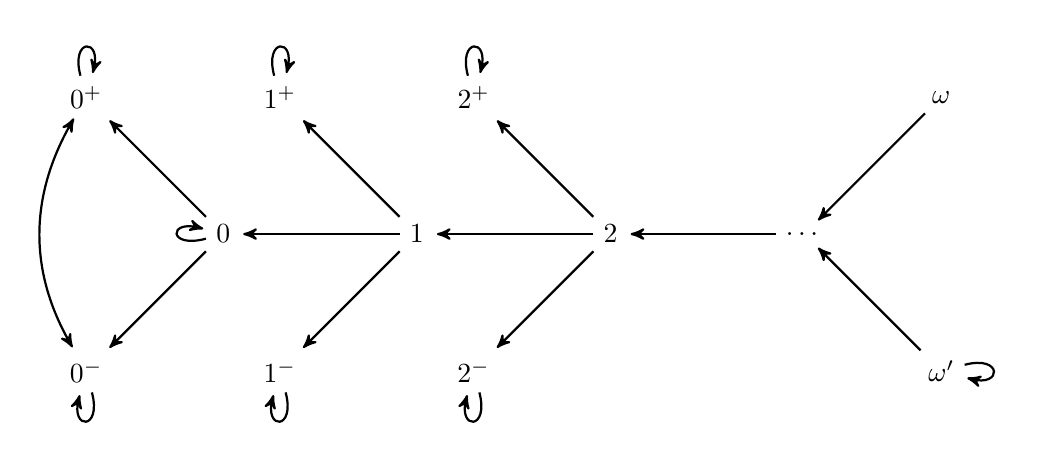
\begin{tikzpicture}[>=stealth',shorten >=1pt,auto,node distance=7em,thick]

      \node (0) {$0$};
      \node (0+) [above left of=0] {$0^+$};
      \node (0-) [below left of=0] {$0^-$};
      \node (1) [right of=0] {$1$};
      \node (1+) [above left of=1] {$1^+$};
      \node (1-) [below left of=1] {$1^-$};
      \node (2) [right of=1] {$2$};
      \node (2+) [above left of=2] {$2^+$};
      \node (2-) [below left of=2] {$2^-$};
      \node (3) [right of=2] {\ldots};
      \node (omega) [above right of=3] {$\omega$};
      \node (omega') [below right of=3] {$\omega'$};

      \path[every node/.style={font=\sffamily\small},->]
        (0) edge [loop left] node {} (0)
            edge node {} (0+)
            edge node {} (0-)
        (0+) edge [loop above] node  {} (0+)
            edge [<->,bend right] node {} (0-)
        (0-) edge [loop below] node  {} (0-)
        (1) edge node {} (0)
            edge node {} (1+)
            edge node {} (1-)
        (1+) edge [loop above] node {} (1+)
        (1-) edge [loop below] node {} (1-)
        (2) edge node {} (1)
            edge node {} (2+)
            edge node {} (2-)
        (2+) edge [loop above] node {} (2+)
        (2-) edge [loop below] node {} (2-)
        (3) edge node {} (2)
        (omega) edge node {} (3)
        (omega') edge node {} (3)
            edge [loop right] node {} (omega');
    \end{tikzpicture}
    \caption{The model $\kModel$, omitting implied transitive edges.}\label{model-caterpillar}
\end{figure}

To show that $\kPModel{\omega}$ and $\kPModel{\omega'}$ are indistinguishable by the refinement modal logic we show that $\kPModel{\omega} \bisimref[n] \kPModel{\omega'}$ for all $n \in \naturals$. To do so we first show that $\kPModel{\omega}$ and $\kPModel{\omega'}$ are mutual refinements.

That $\kPModel{\omega} \refines \kPModel{\omega'}$ is trivial, as $\omega$ is the same as $\omega'$ except for the reflexive edge, so we need only show that $\kPModel{\omega'} \refines \kPModel{\omega}$.

Let $\refinement \subseteq \kStates \times \kStates$ be defined as follows:
\begin{eqnarray*}
\refinement &=& \{(\kStateS, \kStateS) \mid \kStateS \in \kStates\} \cup
    \{(0, \omega), (0, \omega'), (\omega, \omega'), (\omega', \omega)\} \cup  \\&&\quad
    \{(0, n), (n, 0), (0^+, n^+), (0^-, n^-), (\omega, n), (\omega', n) \mid n \in \naturals\}
\end{eqnarray*}

We show that $\refinement$ satisfies {\bf atoms-$\atomP$} and {\bf back} for every $(\kStateS, \kStateSP) \in \refinement$.

\begin{description}
    \item[Case: $(\kStateS, \kStateS) \in \refinement$]\hfill
        \begin{description}
            \item[atoms-$\atomP$]
                Trivial.
            \item[back]
                Let $\kStateT \in \kSuccessors{}{\kStateS}$. 
                By construction $(\kStateT, \kStateT) \in \refinement$.
        \end{description}
    \item[Case: $(0, n) \in \refinement$ where $n \in \naturals$:]\hfill
        \begin{description}
            \item[atoms-$\atomP$]
                By construction $0 \in \kValuation(\atomP)$ and $n \in \kValuation(\atomP)$.
            \item[back]
                Let $k^* \in \kSuccessors{}{n}$.

                Suppose that $k^* = k$ where $k \in \naturals$.
                By construction $0 \in \kSuccessors{}{0}$ and $(0, k) \in \refinement$.

                Suppose that $k^* = k^+$ where $k \in \naturals$.
                By construction $0^+ \in \kSuccessors{}{0}$ and $(0^+, k^+) \in \refinement$.

                Suppose that $k^* = k^-$ where $k \in \naturals$.
                By construction $0^- \in \kSuccessors{}{0}$ and $(0^-, k^-) \in \refinement$.
        \end{description}
    \item[Case: $(n, 0) \in \refinement$ where $n \in \naturals$:]\hfill
        \begin{description}
            \item[atoms-$\atomP$]
                By construction $n \in \kValuation(\atomP)$ and $0 \in \kValuation(\atomP)$.
            \item[back]
                Let $k^* \in \kSuccessors{}{0}$.
                By construction $k^* \in \kSuccessors{}{n}$ and $(k^*, k^*) \in \refinement$.
        \end{description}
    \item[Case: $(0^+, n^+) \in \refinement$ where $n \in \naturals$:]\hfill
        \begin{description}
            \item[atoms-$\atomP$]
                By construction $0^+ \in \kValuation(\atomP)$ and $n^+ \in \kValuation(\atomP)$.
            \item[back]
                Let $n^+ \in \kSuccessors{}{n^+}$.
                By construction $0^+ \in \kSuccessors{}{n^+}$ and $(0^+, n^+) \in \refinement$.
        \end{description}
    \item[Case: $(0^-, n^-) \in \refinement$ where $n \in \naturals$:]\hfill
        \begin{description}
            \item[atoms-$\atomP$]
                By construction $0^- \notin \kValuation(\atomP)$ and $n^- \notin \kValuation(\atomP)$.
            \item[back]
                Let $n^- \in \kSuccessors{}{n^0}$.
                By construction $0^- \in \kSuccessors{}{n^-}$ and $(0^-, n^-) \in \refinement$.
        \end{description}
    \item[Case: $(\omega, n) \in \refinement$ where $n \in \naturals$:]\hfill
        \begin{description}
            \item[atoms-$\atomP$]
                By construction $\omega \in \kValuation(\atomP)$ and $n \in \kValuation(\atomP)$.
            \item[back]
                Let $k^* \in \kSuccessors{}{n}$.
                By construction $k^* \in \kSuccessors{}{\omega}$ and $(k^*, k^*) \in \refinement$.
        \end{description}
    \item[Case: $(\omega', n) \in \refinement$ where $n \in \naturals$:]\hfill
        \begin{description}
            \item[atoms-$\atomP$]
                By construction $\omega' \in \kValuation(\atomP)$ and $n \in \kValuation(\atomP)$.
            \item[back]
                Let $k^* \in \kSuccessors{}{n}$.
                By construction $k^* \in \kSuccessors{}{\omega}$ and $(k^*, k^*) \in \refinement$.
        \end{description}
    \item[Case: $(0, \omega) \in \refinement$:]\hfill
        \begin{description}
            \item[atoms-$\atomP$]
                By construction $0 \in \kValuation(\atomP)$ and $\omega \in \kValuation(\atomP)$.
            \item[back]
                Let $k^* \in \kSuccessors{}{\omega}$.
                Suppose that $k^* = k$ where $k \in \naturals$.
                By construction $0 \in \kSuccessors{}{0}$ and $(0, k) \in \refinement$.

                Suppose that $k^* = k^+$ where $k \in \naturals$.
                By construction $0^+ \in \kSuccessors{}{0}$ and $(0^+, k^+) \in \refinement$.

                Suppose that $k^* = k^-$ where $k \in \naturals$.
                By construction $0^- \in \kSuccessors{}{0}$ and $(0^-, k^-) \in \refinement$.
        \end{description}
    \item[Case: $(0, \omega') \in \refinement$:]\hfill
        \begin{description}
            \item[atoms-$\atomP$]
                By construction $0 \in \kValuation(\atomP)$ and $\omega' \in \kValuation(\atomP)$.
            \item[back]
                Let $k^* \in \kSuccessors{}{\omega'}$.

                Suppose that $k^* = \omega'$.
                By construction $0 \in \kSuccessors{}{\omega'}$ and $(0, \omega') \in \refinement$.

                Suppose that $k^* = k$ where $k \in \naturals$.
                By construction $0 \in \kSuccessors{}{0}$ and $(0, k) \in \refinement$.

                Suppose that $k^* = k^+$ where $k \in \naturals$.
                By construction $0^+ \in \kSuccessors{}{0}$ and $(0^+, k^+) \in \refinement$.

                Suppose that $k^* = k^-$ where $k \in \naturals$.
                By construction $0^- \in \kSuccessors{}{0}$ and $(0^-, k^-) \in \refinement$.
        \end{description}
    \item[Case: $(\omega, \omega') \in \refinement$:]\hfill
        \begin{description}
            \item[atoms-$\atomP$]
                By construction $\omega \in \kValuation(\atomP)$ and $\omega' \in \kValuation(\atomP)$.
            \item[back]
                Let $k^* \in \kSuccessors{}{\omega'}$.

                Suppose that $k^* = \omega'$.
                By construction $0 \in \kSuccessors{}{\omega}$ and $(0, \omega') \in \refinement$.

                Suppose that $k^* \neq \omega'$.
                By construction $k^* \in \kSuccessors{}{\omega}$ and $(k^*, k^*) \in \refinement$.
        \end{description}
    \item[Case: $(\omega', \omega) \in \refinement$:]\hfill
        \begin{description}
            \item[atoms-$\atomP$]
                By construction $\omega' \in \kValuation(\atomP)$ and $\omega \in \kValuation(\atomP)$.
            \item[back]
                Let $k^* \in \kSuccessors{}{\omega}$.
                By construction $k^* \in \kSuccessors{}{\omega'}$ and $(k^*, k^*) \in \refinement$.
        \end{description}
\end{description}

We next show that $\kPModel{\omega} \bisimref[n] \kPModel{\omega'}$ for every $n \in \naturals$. 
To show this we show the following intermediate results for every $n \in \naturals$:
\begin{enumerate}
    \item $\kPModel{i} \bisimref[n] \kPModel{j}$ for $i, j$ where $i, j \geq n$.
    \item $\kPModel{n} \bisimref[n] \kPModel{\omega'}$.
    \item $\kPModel{\omega} \bisimref[n] \kPModel{\omega'}$.
\end{enumerate}

We proceed by induction on $n \in \naturals$.

\begin{enumerate}
    \item We show that $\kPModel{i} \bisimref[n] \kPModel{j}$ for $i, j$ where $i, j \geq n$.

    Suppose that $n = 0$. 
    From above, $\kPModel{i} \refines \kPModel{0} \refines \kPModel{j}$ and $\kPModel{i} \simulates \kPModel{0} \simulates \kPModel{j}$ so we have that $\kPModel{i} \bisimref[0] \kPModel{j}$.

    Suppose that $n > 0$.

    \paragraph{mutual refinements}

    From above, $\kPModel{i} \refines \kPModel{0} \refines \kPModel{j}$
    and $\kPModel{i} \simulates \kPModel{0} \simulates \kPModel{j}$.

    \paragraph{forth}

    Let $k^* \in \kSuccessors{}{i}$.

    Suppose that $k^* = k$ where $k \in \naturals$ and $k \geq n - 1$.
    Then from the induction hypothesis $\kPModel{k} \bisimilar [n-1] \kPModel{j - 1}$.

    Suppose that $k^* = k$ where $k \in \naturals$ and $k < n - 1$.
    Then $k < n - 1 < j$ so $k \in \kSuccessors{}{j}$ and we trivially have that $\kPModel{k} \bisimilar \kPModel{k}$.

    Suppose that $k^* = 0^+$.
    Then $0^+ \in \kSuccessors{}{j}$ and we trivially have that $\kPModel{0^+} \bisimilar \kPModel{0^+}$.

    Suppose that $k^* = k^+$ where $k \in \naturals$ and $k > 0$.
    Then $j^+ \in \kSuccessors{}{j}$ and as $j \geq n > 0$ we trivially have that $\kPModel{k^+} \bisimilar \kPModel{k^+}$.

    Suppose that $k^* = k^-$ for $k \in \naturals$. This follows from similar reasoning to the case where $k^* = k^+$.

    \paragraph{back}

    Symmetrical reasoning to {\bf forth}.

    \item We show that $\kPModel{n} \bisimref[n] \kPModel{\omega'}$.

    Suppose that $n = 0$. 
    From above, $\kPModel{n} \refines \kPModel{0} \refines \kPModel{\omega'}$ and $\kPModel{n} \simulates \kPModel{\omega'}$ so we have that $\kPModel{0} \bisimref[0] \kPModel{\omega'}$.

    Suppose that $n > 0$.

    \paragraph{mutual refinements}

    From above, $\kPModel{n} \refines \kPModel{0} \refines \kPModel{\omega'}$ and $\kPModel{n} \simulates \kPModel{\omega'}$.

    \paragraph{forth}

    Let $k \in \kSuccessors{}{n}$. 
    Then $k \in \kSuccessors{}{\omega'}$ and we trivially have that $\kPModel{k} \bisimilar \kPModel{k}$.

    \paragraph{back}

    Let $k \in \kSuccessors{}{\omega'}$. 

    Suppose that $k = \omega'$. 
    Then $n - 1 \in \kSuccessors{}{n}$ and by the induction hypothesis $\kPModel{n - 1} \bisimilar{n - 1} \kPModel{\omega'}$.

    Suppose that $k \neq \omega'$ and $k < n$. Then $k \in \kSuccessors{}{n}$ and we trivially have that $\kPModel{k} \bisimilar \kPModel{k}$.

    Suppose that $k \geq n$. Then $n - 1 \in \kSuccessors{}{n}$ and from above we have that $\kPModel{k} \bisimref[n - 1] \kPModel{n - 1}$.
    
    \item We show that $\kPModel{\omega} \bisimref[n] \kPModel{\omega'}$.

    Suppose that $n = 0$. 
    From above $\kPModel{\omega} \refines \kPModel{\omega'}$ and  $\kPModel{\omega} \simulates \kPModel{\omega'}$ so we have that $\kPModel{\omega} \bisimref[0] \kPModel{\omega'}$.

    Suppose that $n > 0$.

    \paragraph{mutual refinements}

    From above $\kPModel{\omega} \refines \kPModel{\omega'}$ and  $\kPModel{\omega} \simulates \kPModel{\omega'}$.

    \paragraph{forth}

    Let $k \in \kSuccessors{}{\omega}$.
    Then $k \in \kSuccessors{}{\omega'}$ and we trivially have that $\kPModel{k} \bisimilar \kPModel{k}$.

    \paragraph{back}

    Let $k \in \kSuccessors{}{\omega'}$.

    Suppose that $k = \omega'$.
    Then $n - 1 \in \kSuccessors{}{\omega}$ and from above we have that $\kPModel{n - 1} \bisimref[n - 1] \kPModel{\omega'}$.

    Suppose that $k \neq \omega'$.
    Then $k \in \kSuccessors{}{\omega}$ and we trivially have that $\kPModel{k} \bisimilar \kPModel{k}$.
\end{enumerate}

Therefore $\kPModel{\omega} \bisimref[n] \kPModel{\omega'}$ for every $n \in \naturals$.

Let $\phi \in \langRml$ and let $n = d(\phi)$ be the modal depth of $\phi$.
From above $\kPModel{\omega} \bisimref[n] \kPModel{\omega'}$ so $\kPModel{\omega} \entails \phi$ if and only if $\kPModel{\omega'} \entails \phi$.
Therefore $\kPModel{\omega}$ is refinement modally indistinguishable from $\kPModel{\omega'}$.

We next show that the states $\kPModel{\omega}$ and $\kPModel{\omega'}$ are distinguishable by the modal $\mu$-calculus logic formula $\gfp{\varX} (\possible (\varX \land \possible \necessary \atomP) \land \possible (\varX \land \possible \necessary \neg \atomP))$.
Although we do not show it formally here, this distinguishing formula corresponds to the semantic property that there exists an infinite path starting from the designated state in a pointed Kripke model, along which there is always a successor state on the path where $\possible \necessary \atomP$ is satisfied and there is always a successor state on the path where $\possible \necessary \lnot \atomP$ is satisfied.
It should be clear from the construction of $\kModel$ that $\omega'$ has such a infinite path, consisting of repeatedly following the reflexive edge, whereas $\omega$ does not have such an infinite path, as any infinite path from $\omega$ must include one of the reflexive states, either: a $k^+$ state for $k \in \naturals$, where no successors satisfy $\possible \necessary \lnot \atomP$; a $k^-$ state for $k \in \naturals$, where no successors satisfy $\possible \necessary \atomP$; or $0$, where no successors satisfy either $\possible \necessary \atomP$ or $\possible \necessary \lnot \atomP$.

We proceed with model checking using the modal $\mu$-calculus to show that $\kPModel{\omega}$ and $\kPModel{\omega'}$ disagree on the interpretation of this distinguishing formula.

For any assignment $\kAssignment$ we have the following:
\begin{eqnarray*}
    \interpretation[\kAssignment]{\atomP} &=& \{n, n^+ \mid n \in \naturals\} \cup \{\omega, \omega'\}\\
    \interpretation[\kAssignment]{\necessary \atomP} &=& \{n^+ \mid n \in \naturals, n > 0\}\\
    \interpretation[\kAssignment]{\possible \necessary \atomP} &=& \{n, n^+ \mid n \in \naturals, n > 0\} \cup \{\omega, \omega'\}\\
    \interpretation[\kAssignment]{\neg \atomP} &=& \{n^- \mid n \in \naturals\}\\
    \interpretation[\kAssignment]{\necessary \neg \atomP} &=& \{n^- \mid n \in \naturals, n > 0\}\\
    \interpretation[\kAssignment]{\possible \necessary \neg \atomP} &=& \{n, n^- \mid n \in \naturals, n > 0\} \cup \{\omega, \omega'\}
\end{eqnarray*}

For any assignment $\kAssignment$ where $\kAssignment(\varX) = \kStates$ we have the following:
\begin{eqnarray*}
    \interpretation[\kAssignment]{\varX} &=& \kStates\\
    \interpretation[\kAssignment]{\varX \land \possible \necessary \atomP} &=& \{n, n^+ \mid n \in \naturals, n > 0\} \cup \{\omega, \omega'\}\\
    \interpretation[\kAssignment]{\possible (\varX \land \possible \necessary \atomP)} &=& \{n, n^+ \mid n \in \naturals, n > 0\} \cup \{\omega, \omega'\}\\
    \interpretation[\kAssignment]{\varX \land \possible \necessary \neg \atomP} &=& \{n, n^- \mid n \in \naturals, n > 0\} \cup \{\omega, \omega'\}\\
    \interpretation[\kAssignment]{\possible (\varX \land \possible \necessary \neg \atomP)} &=& \{n, n^- \mid n \in \naturals, n > 0\} \cup \{\omega, \omega'\}\\
    \interpretation[\kAssignment]{\possible (\varX \land \possible \necessary \atomP) \land \possible (\varX \land \possible \necessary \neg \atomP)} &=& \{n \mid n \in \naturals, n > 0\} \cup \{\omega, \omega'\}
\end{eqnarray*}

For any assignment $\kAssignment$ where $\kAssignment(\varX) = \{n \mid n \in \naturals, n > m\} \cup \{\omega, \omega'\}$ for some $m \in \naturals$ we have the following:
\begin{eqnarray*}
    \interpretation[\kAssignment]{\varX} &=& \{n \mid n \in \naturals, n > m\} \cup \{\omega, \omega'\}\\
    \interpretation[\kAssignment]{\varX \land \possible \necessary \atomP} &=& \{n \mid n \in \naturals, n > m\} \cup \{\omega, \omega'\}\\
    \interpretation[\kAssignment]{\possible (\varX \land \possible \necessary \atomP)} &=& \{n \mid n \in \naturals, n > m + 1\} \cup \{\omega, \omega'\}\\
    \interpretation[\kAssignment]{\varX \land \possible \necessary \neg \atomP} &=& \{n \mid n \in \naturals, n > m\} \cup \{\omega, \omega'\}\\
    \interpretation[\kAssignment]{\possible (\varX \land \possible \necessary \neg \atomP)} &=& \{n \mid n \in \naturals, n > m + 1\} \cup \{\omega, \omega'\}\\
    \interpretation[\kAssignment]{\possible (\varX \land \possible \necessary \atomP) \land \possible (\varX \land \possible \necessary \neg \atomP)} &=& \{n \mid n \in \naturals, n > m + 1\} \cup \{\omega, \omega'\}
\end{eqnarray*}

For any assignment $\kAssignment$ where $\kAssignment(\varX) = \{\omega, \omega'\}$ for some $m \in \naturals$ we have the following:
\begin{eqnarray*}
    \interpretation[\kAssignment]{\varX} &=& \{\omega, \omega'\}\\
    \interpretation[\kAssignment]{\varX \land \possible \necessary \atomP} &=& \{\omega, \omega'\}\\
    \interpretation[\kAssignment]{\possible (\varX \land \possible \necessary \atomP)} &=& \{\omega'\}\\
    \interpretation[\kAssignment]{\varX \land \possible \necessary \neg \atomP} &=& \{\omega, \omega'\}\\
    \interpretation[\kAssignment]{\possible (\varX \land \possible \necessary \neg \atomP)} &=& \{\omega'\}\\
    \interpretation[\kAssignment]{\possible (\varX \land \possible \necessary \atomP) \land \possible (\varX \land \possible \necessary \neg \atomP)} &=& \{\omega'\}
\end{eqnarray*}

Therefore for any assignment $\kAssignment$ we have that: $$\interpretation[\kAssignment]{\gfp{\varX} (\possible (\varX \land \possible \necessary \atomP) \land \possible (\varX \land \possible \necessary \neg \atomP))} = \{\omega'\}$$

Therefore $\kPModel{\omega'} \entails \gfp{\varX} (\possible (\varX \land \possible \necessary \atomP) \land \possible (\varX \land \possible \necessary \neg \atomP))$, 
but $\kPModel{\omega} \nentails \gfp{\varX} (\possible (\varX \land \possible \necessary \atomP) \land \possible (\varX \land \possible \necessary \neg \atomP))$.

Therefore $\kPModel{\omega}$ is distinguishable from $\kPModel{\omega'}$ using the modal $\mu$-calculus.

Therefore \logicRmlKF{} is strictly less expressive than \logicMuKF{}.
\end{proof}

As \logicMuKF{} is expressively equivalent to \logicBqmlKF{} we also trivially get the following corollary. 

\begin{corollary}
The logic \logicRmlKF{} is strictly less expressive than \logicBqmlKF{}.
\end{corollary}

    \chapter{Arbitrary action model logic}\label{aaml}

In this chapter we introduce the arbitrary action model logic (\logicAaml{}) and consider results specific to the settings of \classK{}, \classKFF{}, and \classS{}.
\logicAaml{} extends the action model logic of Baltag, Moss and Solecki~\cite{baltag:1998,baltag:2004} with quantifiers that denote either that every action model results in a statement becoming true or that some action model results in a statement becoming true.
This formulation was proposed by Balbiani, et al.~\cite{balbiani:2007} as a possible generalisation for \logicApal{}, and is similar to how the arbitrary public announcement logic of Balbiani, et al~\cite{balbiani:2008} extends public announcement logic.
The main results of this chapter are to show that the action model quantifiers of \logicAaml{} are equivalent to the refinement quantifiers of \logicRml{} in the settings of \classK{}, \classKFF{}, and \classS{}.
As a consequence, most of the results for \logicRml{} from the previous chapters also hold in \logicAaml{} in these settings.
We show the equivalence by showing that if there exists a refinement where a given formula is satisfied then we can construct a finite action model that results in that formula being satisfied.
This equivalence further justifies our interpretation of refinement quantifiers as quantifiers for epistemic updates.
In Section~\ref{aaml-semantics} we introduce the syntax and semantics of \logicAaml{}.
In Section~\ref{aaml-k}, Section~\ref{aaml-kd45}, and Section~\ref{aaml-s5} we consider \logicAaml{} in greater detail in the settings of \classK{}, \classKFF{}, and \classS{} respectively.
In each setting we show that the action model quantifiers of \logicAaml{} are equivalent to the refinement quantifiers of \logicRml{}.

\section{Syntax and semantics}\label{aaml-semantics}

In this section we introduce the syntax and semantics of the arbitrary action model logic.
Like our treatment of \logicRml{}, we consider \logicAaml{} in different settings, including \classK{}, \classKFF{}, and \classS{}.
The definitions that we give here generalise to these different settings.
Unlike our treatment of \logicRml{}, we don't give any semantic results that are common to all of these settings.
As our main results in \logicAaml{} are to show that the action model quantifiers of \logicAaml{} are equivalent to the refinement quantifiers of \logicRml{} in the settings we consider, all of the semantic results from \logicRml{} also apply to \logicAaml{} in these settings.
For the same reason we use the same syntax for action model quantifiers and refinement quantifiers.

We begin with a definition of the syntax of \logicAaml{}.
As in action model logic, the syntax of \logicAaml{} is parameterised by a class of Kripke models, \classC{}, and a set of action signatures, \aSignatureFamily{}.

\begin{definition}[Language of arbitrary action model logic]
Let \aSignatureFamily{} be a non-empty, countable set of action signatures.
The {\em language of arbitrary action model logic} with action signatures \aSignatureFamily{}, $\langAaml(\aSignatureFamily)$, is inductively defined as:
$$
\phi ::= 
    \atomP \mid
    \lnot \phi \mid
    (\phi \land \phi) \mid
    \necessaryA \phi \mid
    \actionA{\aSignature \aStatesT, \phi, \dots, \phi} \phi \mid
    \allactsBs \phi
$$
where $\atomP \in \atoms$, $\agentA \in \agents$, $\agentsB \subseteq \agents$, $\aSignatureAndTuple \in \aSignatureFamily$, $\aStatesT \subseteq \aStates$, and the number of parameters to a given action signature $\aSignature$ is determined by the number of designated actions in the action signature.
\end{definition}

We use all of the standard abbreviations from modal logic, in addition to the abbreviations $\somerefsBs \phi ::= \lnot \allrefsBs \lnot \phi$, $\allrefs \phi ::= \allrefsAs \phi$, and $\allrefsA \phi ::= \allrefs[\{\agentA\}] \phi$.

The formula $\allacts \phi$ may be read as ``every action model results in $\phi$ becoming true'' and the formula $\someacts \phi$ may be read as ``some action model results in $\phi$ becoming true''.

The use of the subscript $\agentsB$ in the quantifiers $\allactsBs$ and $\someactsBs$ restricts the action models under consideration to action models that result in a $\agentsB$-refinement of the original Kripke model.
The formula $\allactsBs \phi$ may be read as ``every action model results in $\phi$ becoming true if it results in a $\agentsB$-refinement'' and the formula $\someactsBs \phi$ may be read as ``some action model results in $\phi$ becoming true and results in a $\agentsB$-refinement''.
This addition is for the purposes of showing a full correspondence between action model quantifiers and refinement quantifiers.
Although we do not consider it in greater detail here, the notion of restricting the results of executing action models to $\agentsB$-refinements seems like it would be useful.
For example, $\agentsB$-refinements can be partially characterised as those Kripke models that preserve the truth of $\agentsB$-positive formulas, restricting the learning of new information to agents in $\agentsB$.
So an alternative reading of the formula $\allactsBs \phi$ may be ``every action model where only agents in $\agentsB$ learn new information results in $\phi$ becoming true'' and an alternative reading of the formula $\someactsBs \phi$ may be ``some action model where only agents in $\agentsB$ learn new information results in $\phi$ becoming true''.

We define the semantics of \logicAaml{}.

\begin{definition}[Semantics of arbitrary action model logic]
Let \classC{} be a class of Kripke models and let \aSignatureFamily{} be a non-empty, countable set of action signatures, let $\phi \in \langAaml(\aSignatureFamily)$, and let $\kPModelAndTuple{\kStateS} \in \classC$ be a pointed Kripke model.
The interpretation of the formula $\phi$ in the logic \logicAamlC{} on the pointed Kripke model $\kPModel{\kStateS}$ is the same as its interpretation in action model logic, defined in Definition~\ref{aml-semantics}, with the additional inductive case:
$$
\begin{array}{lcl}
  \kPModel{\kStateS} \entails \allactsBs \phi & \text{ iff } & \text{for every } \aPModel{\aStateS} \in \aSignatureFamily \text{ such that } \aPrecondition \subseteq \langMl\\&&\quad \text{ if } \kPModel{\kStateS} \entails \aPrecondition(\aStateS) \text{ and } \kPModel{\kStateS} \simulatesBs \kPModel{\kStateS} \exec \aPModel{\aStateS}\\&&\quad \text{ then } \kPModel{\kStateS} \exec \aPModel{\aStateS} \entails \phi
\end{array}
$$
\end{definition}

\pagebreak

We are interested in the following variants of arbitrary action model logic:
\begin{itemize}
    \item \logicAamlK{} interpreted over the class of \classK{} Kripke frames and the language of arbitrary action model logic $\langAaml(\classK)$ with action signatures defined on the class of finite \classK{} Kripke frames.
    \item \logicAamlKFF{} interpreted over the class of \classKFF{} Kripke frames and the language of arbitrary action model logic $\langAaml(\classKFF)$ with action signatures defined on the class of finite \classKFF{} Kripke frames.
    \item \logicAamlS{} interpreted over the class of \classS{} Kripke frames and the language of arbitrary action model logic $\langAaml(\classS)$ with action signatures defined on the class of finite \classS{} Kripke frames.
\end{itemize}

We note that by Proposition~\ref{action-models-refinements} the result of executing any action model is a $\agents$-refinement, so the action model quantifiers $\allactsAs$ and $\someactsAs$, abbreviated as $\allacts$ and $\someacts$ respectively, correspond to unrestricted action model quantification.
Given this we can observe that the semantics of the action model quantifier $\allacts$ is similar to the semantics of the public announcement quantifier of \logicApal{}~\cite{balbiani:2007}.
Whilst \logicApal{} permits public announcements of formulas containing public announcement quantifiers, the public announcement quantifiers do not quantify over public announcements that themselves contain quantifiers.
This is required to ensure the well-foundedness of the semantics of the logic.
We make a similar restriction here with the semantics of \logicAaml{}.
However we will show in the following sections that such a restriction is unnecessary in the settings that we consider; the logics \logicAamlK{}, \logicAamlKFF{}, and \logicAamlS{} are expressively equivalent to their underlying modal logics, \logicK{}, \logicKFF{}, and \logicS{} respectively, so any action model containing quantifiers is equivalent to an action model without quantifiers.
Despite the action model quantifiers quantifying over more epistemic updates that public announcement quantifiers, the public announcement quantifiers are in fact more powerful than action model quantifiers, at least in the setting of \classS{}, as \logicApalS{} is strictly more expressive than \logicS{} and is undecidable, whereas \logicAamlS{} is expressively equivalent to \logicS{} and is decidable.

We give some examples of \logicAaml{}.

\begin{example}
Let $\kPModelAndTuple{\kStateS}$ and $\kPModelAndTupleP{\kStateS}$ be Kripke models where:
\begin{eqnarray*}
    \kStates &=& \{\kStateS, \kStateT\}\\
    \kAccessibilityA &=& \{(\kStateS, \kStateS), (\kStateT, \kStateT)\}\\
    \kAccessibilityB &=& \{(\kStateS, \kStateS), (\kStateS, \kStateT), (\kStateT, \kStateS), (\kStateT, \kStateT)\}\\
    \kValuation(\atomP) &=& \{\kStateS\}
\end{eqnarray*}
and:
\begin{eqnarray*}
    \kStatesP &=& \{\kStateS, \kStateT, \kStateU\}\\
    \kAccessibilityPA &=& \{(\kStateS, \kStateS), (\kStateT, \kStateT), (\kStateS, \kStateU), (\kStateU, \kStateS), (\kStateU, \kStateU)\}\\
    \kAccessibilityPB &=& \{(\kStateS, \kStateS), (\kStateS, \kStateT), (\kStateT, \kStateS), (\kStateT, \kStateT), (\kStateU, \kStateU)\}\\
    \kValuationP(\atomP) &=& \{\kStateS, \kStateU\}
\end{eqnarray*}

\begin{figure}
    \caption{Two Kripke models that are each the result of executing an action model on the other.}\label{example-aaml-figure}
    \centering
    \begin{tikzpicture}[>=stealth',shorten >=1pt,auto,node distance=7em,thick]

      \node[label=above right:{$\kStateS$}] (s') {\underline{$\{\atomP\}$}};
      \node[label=above right:{$\kStateT$}] (t') [above of=s'] {$\{\}$};
      \node[label=above:{$\kPModel{\kStateS}$},draw=black, fit=(s') (t'), inner sep=3.5em, dashed, rounded corners] {};

      \path[every node/.style={font=\sffamily\small},->]
        (s') edge [loop right] node {$\agentA, \agentB$} (s')
        (t') edge [loop right] node {$\agentA, \agentB$} (t')
        (s') [<->] edge node {$\agentB$} (t');

      \node[label=above left:{$\kStateS$}] (s) [right=11em of s] {\underline{$\{\atomP\}$}};
      \node[label=above left:{$\kStateT$}] (t) [above of=s] {$\{\}$};
      \node[label=above left:{$\kStateU$}] (u) [below of=s] {$\{\atomP\}$};
      \node[label=above:{$\kPModelP{\kStateS}$},draw=black, fit=(s) (t) (u), inner sep=3.5em, dashed, rounded corners] {};

      \path[every node/.style={font=\sffamily\small},->]
        (s) edge [loop left] node {$\agentA, \agentB$} (s)
        (t) edge [loop left] node {$\agentA, \agentB$} (t)
        (u) edge [loop left] node {$\agentA, \agentB$} (u)
        (s) [<->] edge node {$\agentB$} (t)
        (s) edge node {$\agentA$} (u);
    \end{tikzpicture}
\end{figure}

The Kripke models $\kPModel{\kStateS}$ and $\kPModelP{\kStateS}$ are shown in Figure~\ref{example-aaml-figure}.
We note that $\kPModel{\kStateS}$ and $\kPModelP{\kStateS}$ are essentially the same as (are isomorphic to) the Kripke models from Example~\ref{example-pal-ml} and Example~\ref{example-pal}.
In Example~\ref{example-pal-ml} we showed that $\kPModelP{\kStateS}$ is the result of executing an action model on $\kPModel{\kStateS}$, and in Example~\ref{example-pal} we showed that $\kPModel{\kStateS}$ is the result of executing an action model on $\kPModelP{\kStateS}$.

We note that $\kPModelP{\kStateS} \entails_\logicAamlK \knowsA \lnot \knowsB \atomP$.
As $\kPModelP{\kStateS}$ is the result of executing an action model on $\kPModel{\kStateS}$ we have that $\kPModel{\kStateS} \entails_\logicAamlK \someacts \knowsA \lnot \knowsB \atomP$.

We note that $\kPModel{\kStateS} \entails_\logicAamlK \lnot \knowsA \lnot \knowsB \atomP$.
As $\kPModel{\kStateS}$ is the result of executing an action model on $\kPModelP{\kStateS}$ we have that $\kPModel{\kStateS} \entails_\logicAamlK \someacts \lnot \knowsA \lnot \knowsB \atomP$.
\end{example}

\begin{example}
Let $\kPModelAndTuple{\kStateS}$ and $\kPModelAndTupleP{\kStateS}$ be Kripke models where:
\begin{eqnarray*}
    \kStates &=& \{\kStateS, \kStateT, \kStateU, \kStateV\}\\
    \kAccessibilityA &=& \{(\kStateS, \kStateS), (\kStateS, \kStateT), (\kStateT, \kStateS), (\kStateT, \kStateT), (\kStateU, \kStateU), (\kStateU, \kStateV), (\kStateV, \kStateU), (\kStateV, \kStateV)\}\\
    \kAccessibilityB &=& \{(\kStateS, \kStateS), (\kStateS, \kStateU), (\kStateU, \kStateS), (\kStateU, \kStateU), (\kStateT, \kStateT), (\kStateT, \kStateV), (\kStateV, \kStateT), (\kStateV, \kStateV)\}\\
    \kValuation(\atomP) &=& \{\kStateS, \kStateT\}\\
    \kValuation(\atomQ) &=& \{\kStateS, \kStateU\}
\end{eqnarray*}
and:
\begin{eqnarray*}
    \kStates &=& \{\kStateS, \kStateT\}\\
    \kAccessibilityA &=& \{(\kStateS, \kStateS), (\kStateS, \kStateT), (\kStateT, \kStateS), (\kStateT, \kStateT)\}\\
    \kAccessibilityB &=& \{(\kStateS, \kStateS), (\kStateT, \kStateT)\}\\
    \kValuation(\atomP) &=& \{\kStateS, \kStateT\}\\
    \kValuation(\atomQ) &=& \{\kStateS\}
\end{eqnarray*}

\begin{figure}
    \caption{An example of a Kripke model and the result of executing an action model.}\label{example-aaml-2-figure}
    \centering
    \begin{tikzpicture}[>=stealth',shorten >=1pt,auto,node distance=7em,thick]

      \node[label=above right:{$\kStateS$}] (s) {\underline{$\{\atomP, \atomQ\}$}};
      \node[label=below right:{$\kStateT$}] (t) [below of=s] {$\{\atomP\}$};
      \node[label=above left:{$\kStateU$}] (u) [left of=s] {$\{\atomQ\}$};
      \node[label=below left:{$\kStateV$}] (v) [left of=t] {$\{\}$};
      \node[label=above:{$\kPModel{\kStateS}$},draw=black, fit=(s) (t) (u) (v), inner sep=3em, dashed, rounded corners] {};

      \path[every node/.style={font=\sffamily\small},->]
        (s) edge [loop above] node {$\agentA, \agentB$} (s)
        (t) edge [loop below] node {$\agentA, \agentB$} (t)
        (u) edge [loop above] node {$\agentA, \agentB$} (u)
        (v) edge [loop below] node {$\agentA, \agentB$} (v)
        (s) [<->] edge node {$\agentA$} (t)
        (u) [swap] edge node {$\agentA$} (v)
        (s) edge node {$\agentB$} (u)
        (t) [swap] edge node {$\agentB$} (v);

      \node[label=above left:{$\kStateS$}] (s') [right=9em of s]{\underline{$\{\atomP, \atomQ\}$}};
      \node[label=below left:{$\kStateT$}] (t') [below of=s'] {$\{\atomP\}$};
      \node[label=above:{$\restrict{\kPModel{\kStateS}}{\knowsA \atomP}$},draw=black, fit=(s') (t'), inner sep=3em, dashed, rounded corners] {};

      \path[every node/.style={font=\sffamily\small},->]
        (s') edge [loop above] node {$\agentA, \agentB$} (s')
        (t') edge [loop below] node {$\agentA, \agentB$} (t')
        (s') [<->] edge node {$\agentA$} (t');
    \end{tikzpicture}
\end{figure}

The Kripke models $\kPModel{\kStateS}$ and $\kPModelP{\kStateS}$ are shown in Figure~\ref{example-aaml-2-figure}.
We note that $\kPModel{\kStateS}$ and $\kPModelP{\kStateS}$ are essentially the same as (are isomorphic to) the Kripke models from Example~\ref{example-pal}.
In Example~\ref{example-pal} we showed that $\kPModelP{\kStateS}$ is the result of executing an action model on $\kPModel{\kStateS}$.

We note that $\kPModelP{\kStateS} \entails_\logicAamlK \knowsA \atomP$.
Let $\aPModel{\aStateS} \in \classAmK$ such that $\kPModelP{\kStateS} \entails_\logicAamlK \aPrecondition(\aStateS)$.
By Proposition~\ref{action-models-refinements} we have that $\kPModelP{\kStateS} \simulates \kPModelP{\kStateS} \exec \aPModel{\aStateS}$.
As $\knowsA \atomP$ is a positive formula and $\kPModelP{\kStateS} \simulates \kPModelP{\kStateS} \exec \aPModel{\aStateS}$, from Proposition~\ref{refinements-preserve-positive} we that $\kPModelP{\kStateS} \exec \aPModel{\aStateS} \entails_\logicAamlK \knowsA \atomP$.
Therefore $\kPModelP{\kStateS} \entails_\logicAamlK \allacts \knowsA \atomP$.
As $\kPModelP{\kStateS}$ is the result of executing an action model in $\kPModel{\kStateS}$ we have that $\kPModel{\kStateS} \entails_\logicAamlK \someacts \allacts \knowsA \atomP$.
\end{example}

\pagebreak

In the following sections we show that the action model quantifiers of \logicAaml{} are equivalent to the refinement quantifiers of \logicRml{} in the settings of \classK{}, \classKFF{}, and \classS{}.
We show the equivalence by showing that if there exists a refinement where a given formula is satisfied then we can construct a finite action model that results in that formula being satisfied.
We have already shown the converse: if there exists an action model that results in a given formula being satisfied then by Proposition~\ref{action-models-refinements} the result of executing the action model is itself a refinement, so there exists a refinement where the formula is satisfied.
We rely heavily on results from action model logic and \logicRml{}, particularly the axioms from both, so we find it useful to define a logic, which we call refinement action model logic (\logicRaml{}), that extends action model logic with refinement quantifiers.

\begin{definition}[Semantics of refinement action model logic]
Let \classC{} be a class of Kripke models and let \aSignatureFamily{} be a non-empty, countable set of action signatures, let $\phi \in \langAaml(\aSignatureFamily)$, and let $\kPModelAndTuple{\kStateS} \in \classC$ be a pointed Kripke model.
The interpretation of the formula $\phi$ in the logic \logicRamlC{} on the pointed Kripke model $\kPModel{\kStateS}$ is the same as its interpretation in action model logic, defined in Definition~\ref{aml-semantics}, with the additional inductive case:
$$
\begin{array}{lcl}
    \kPModel{\kStateS} \entails \allactsBs \phi & \text{ iff } & \text{for every } \kPModelP{\kStateSP} \in \classC \text{ if } \kPModel{\kStateS} \simulatesBs \kPModelP{\kStateSP} \text{ then } \kPModelP{\kStateSP} \entails \phi
\end{array}
$$
\end{definition}

As with \logicAaml{} we are interested in the following variants of refinement action model logic:
\begin{itemize}
    \item \logicRamlK{} interpreted over the class of \classK{} Kripke frames and the language of arbitrary action model logic $\langAaml(\classK)$ with action signatures defined on the class of finite \classK{} Kripke frames.
    \item \logicRamlKFF{} interpreted over the class of \classKFF{} Kripke frames and the language of arbitrary action model logic $\langAaml(\classKFF)$ with action signatures defined on the class of finite \classKFF{} Kripke frames.
    \item \logicRamlS{} interpreted over the class of \classS{} Kripke frames and the language of arbitrary action model logic $\langAaml(\classS)$ with action signatures defined on the class of finite \classS{} Kripke frames.
\end{itemize}

In the following sections we will show that results from action model logic and \logicRml{} apply to the combined logic \logicRaml{}, and use these results to show that formulas of \langAaml{} have the same interpretation in both \logicAaml{} and \logicRaml{}.
Unless otherwise noted we will the semantics of \logicRaml{} for our definitions and results, except where we relate \logicRaml{} back to \logicAaml{}.

\pagebreak

\section{K}

\section{K45}

\begin{definition}[Axiomatisation \axiomAamlKFF{}]
The axiomatisation \axiomAamlKFF{} is a substitution schema consisting of the axioms and rules of \axiomAmlKFF{} and the axioms and rules of \axiomRmlKFF{}.
\end{definition}

\begin{theorem}
The axiomatisation \axiomRmlKFF{} is sound and strongly complete with respect to the semantics of the logic \logicAamlKFF{}.
\end{theorem}

\begin{proof}
Soundness of the axioms and rules from \axiomAmlKFF{} and \axiomRmlKFF{} follow from the same reasoning used to show that they are sound in \logicAmlKFF{} and \logicRmlKFF{} respectively.
Strong completeness follows from similar reasoning as in the proof of strong completeness of \axiomAamlK{} in Theorem~\ref{aaml-k-sound-complete}.
\end{proof}

\begin{corollary}
The logic \logicAamlKFF{} is expressively equivalent to the logic \logicKFF{}.
\end{corollary}

\begin{corollary}
The logic \logicAamlKFF{} is compact.
\end{corollary}

\begin{corollary}
The satisfiability problem for the logic \logicAamlKFF{} is decidable.
\end{corollary}

\begin{lemma}
Let $\agentsB \subseteq \agents$, 
let $\phi = \alpha \lor \beta \in \langAaml$, and 
let $\aPModelAndTuple[\alpha]{\aStatesT[\alpha]} \in \classAmKFF$ and $\aPModelAndTuple[\beta]{\aStatesT[\beta]} \in \classAmKFF$ be $\agentsB$-restricted action models such that 
$\entails \actionA{\aPModel[\alpha]{\aStatesT[\alpha]}} \alpha$, 
$\entails \actionE{\aPModel[\alpha]{\aStatesT[\alpha]}} \alpha \iff \someactsBs \alpha$, 
$\entails \actionA{\aPModel[\beta]{\aStatesT[\beta]}} \beta$, and 
$\entails \actionE{\aPModel[\beta]{\aStatesT[\beta]}} \beta \iff \someactsBs \beta$.
Then there exists a $\agentsB$-restricted action model $\aPModel{\aStatesT} \in \classAmKFF$ such that 
$\entails \actionA{\aPModel{\aStatesT}} \phi$, and 
$\entails \actionE{\aPModel{\aStatesT}} \phi \iff \someactsBs \phi$.
\end{lemma}

\begin{lemma}
Let $\agentsB, \agentsC \subseteq \agents$, 
let $\phi = \pi \land \bigwedge_{\agentC \in \agentsC} \coverC \Gamma_\agentC \in \langAaml$ where $\pi \in \langPl$, and 
for every $\agentC \in \agentsC$, $\gamma \in \agentsC$
let $\aPModelAndTuple[\gamma]{\aStatesT[\gamma]} \in \classAmKFF$ be a $\agentsB$-restricted action model such that 
$\entails \actionA{\aPModel[\gamma]{\aStatesT[\gamma]}} \gamma$, and 
$\entails \actionE{\aPModel[\gamma]{\aStatesT[\gamma]}} \gamma \iff \someactsBs \gamma$.
Then there exists a $\agentsB$-restricted action model $\aPModel{\aStatesT} \in \classAmKFF$ such that 
$\entails \actionA{\aPModel{\aStatesT}} \phi$, and 
$\entails \actionE{\aPModel{\aStatesT}} \phi \iff \someactsBs \phi$.
\end{lemma}

\begin{theorem}
Let $\agentsB \subseteq \agents$ and let $\phi \in \langAaml$.
There exists a $\agentsB$-restricted action model $\aPModel{\aStatesT} \in \classAmKFF$ such that 
$\entails \actionA{\aPModel{\aStatesT}} \phi$, and 
$\entails \actionE{\aPModel{\aStatesT}} \phi \iff \someactsBs \phi$.
\end{theorem}

\begin{corollary}
The semantics of \logicAamlK{} as defined in Definition~\ref{aaml-semantics} and the alternative semantics of Definition~\ref{aaml-semantics-alt} are equivalent.
\end{corollary}

\section{S5}\label{aaml-s5}

In this section we consider results specific to the logic \logicAamlS{} in the setting of \classS{}.
This setting is significant as it is the traditional setting for epistemic logic and dynamic epistemic logic.
The main result of this section is that the action model quantifiers of \logicAamlS{} are equivalent to the refinement quantifiers of \logicRmlS{}.
We show this equivalence by showing that if there exists a refinement where a given formula is satisfied then we can construct a finite action model that results in that formula being satisfied.

As in the previous sections, we rely heavily on results from the action model logic \logicAmlS{} and the refinement modal logic \logicRmlS{}, particularly the axioms from both.
We use the combined refinement action model logic \logicRamlS{} so that we can use results from \logicAmlS{} and \logicRmlS{} with a combined syntax, semantics and proof theory.

We first note that as the syntax and semantics of \logicRamlS{} are formed by combining the semantics of \logicAmlS{} and \logicRmlS{}, then \logicAmlS{} and \logicRmlS{} agree with \logicRamlS{} on formulas from their respective sublanguages.

\begin{lemma}\label{raml-s5-aml}
The logics \logicRamlS{} and \logicAmlS{} agree on all formulas of \langAml{}.
That is, for every $\phi \in \langAml$, $\kPModel{\kStateS} \in \classS$: $\kPModel{\kStateS} \entails_\logicRamlS \phi$ if and only if $\kPModel{\kStateS} \entails_\logicAmlS \phi$.
\end{lemma}

\begin{lemma}\label{raml-s5-rml}
The logics \logicRamlS{} and \logicAmlS{} agree on all formulas of \langRml{}.
That is, for every $\phi \in \langRml$, $\kPModel{\kStateS} \in \classS$: $\kPModel{\kStateS} \entails_\logicRamlS \phi$ if and only if $\kPModel{\kStateS} \entails_\logicRmlS \phi$.
\end{lemma}

These results follow directly from the definitions.
We note that these results only apply for \langAml{} and \langRml{} formulas respectively, and do not consider \langAaml{} formulas that contain both action model operators and quantifiers. 

Given this we can give a sound and complete axiomatisation for \logicRamlS{} by combining the axiomatisations for \logicAmlS{} and \logicRmlS{}.

\begin{definition}[Axiomatisation \axiomRamlS{}]\label{raml-s5-axiomatisation}
The axiomatisation \axiomRamlS{} is a substitution schema consisting of the axioms and rules of \axiomAmlS{} and the axioms and rules of \axiomRmlS{}:
$$
\begin{array}{rl}
    {\bf P}     & \text{All propositional tautologies}\\
    {\bf K}     & \proves \necessaryA (\phi \implies \psi) \implies (\necessaryA \phi \implies \necessaryA \psi)\\
    {\bf T}     & \proves \necessaryA \phi \implies \phi\\
    {\bf 5}     & \proves \possibleA \phi \implies \necessaryA \possibleA \phi\\
    {\bf AP} & \proves \actionA{\aPModel{\aStateS}} \atomP \iff (\aPrecondition(\aStateS) \implies \atomP)\\
    {\bf AN} & \proves \actionA{\aPModel{\aStateS}} \lnot \phi \iff (\aPrecondition(\aStateS) \implies \lnot \actionA{\aPModel{\aStateS}} \phi)\\
    {\bf AC} & \proves \actionA{\aPModel{\aStateS}} (\phi \land \psi) \iff (\actionA{\aPModel{\aStateS}} \phi \land \actionA{\aPModel{\aStateS}} \psi)\\
    {\bf AK} & \proves \actionA{\aPModel{\aStateS}} \necessaryA \phi \iff (\aPrecondition(\aStateS) \implies \necessaryA \bigwedge_{\aStateT \in \aSuccessorsA{\aStateS}} \actionA{\aPModel{\aStateT}} \phi)\\
    {\bf AU} & \proves \actionA{\aPModel{\aStatesT}} \phi \iff \bigwedge_{\aStateT \in \aStatesT} \actionA{\aPModel{\aStateT}} \phi\\
    {\bf R} & \proves \allrefsBs (\phi \implies \psi) \implies (\allrefsBs \phi \implies \allrefsBs \psi)\\
    {\bf RP} & \proves \allrefsBs \pi \iff \pi\\
    {\bf RS5} & \proves \somerefsBs (\gamma_0 \land \coversA \Gamma_\agentA) \iff (\somerefsBs \gamma_0 \land \bigwedge_{\gamma \in \Gamma_\agentA} \possibleA \somerefsBs \gamma) \text{ where } \agentA \in \agentsB\\
    {\bf RComm} & \proves \somerefsBs (\gamma_0 \land \coversA \Gamma_\agentA) \iff (\somerefsBs \gamma_0 \land \coversA \{\somerefsBs \gamma \mid \gamma \in \Gamma_\agentA\}) \text{ where } \agentA \notin \agentsB\\
    {\bf RDist} & \proves \somerefsBs (\gamma_0 \land \bigwedge_{\agentA \in \agents} \coversA \Gamma_\agentA) \iff \bigwedge_{\agentA \in \agents} \somerefsBs (\gamma_0 \land \coversA \Gamma_\agentA)\\
    {\bf MP}    & \text{From } \proves \phi \implies \psi \text{ and } \proves \phi \text{ infer } \proves \psi\\
    {\bf NecK}  & \text{From } \proves \phi \text{ infer } \proves \necessaryA \phi\\
    {\bf NecA} & \text{From } \proves \phi \text{ infer } \proves \actionA{\aPModel{\aStatesT}} \phi\\
    {\bf NecR} & \text{From } \proves \phi \text{ infer } \proves \allrefsBs \phi
\end{array}
$$
where $\phi, \psi \in \langAaml$, $\agentA \in \agents$, $\aPModel{\aStateS} \in \classAmS$, $\atomP \in \atoms$, $\pi \in \langPl$, $\agentsB, \agentsC \subseteq \agents$, $\gamma_0 \land \bigwedge_{\agentA \in \agents} \coversA \Gamma_\agentA$ is an explicit formula and for every $\agentA \in \agents$, $\gamma_0 \land \coversA \Gamma_\agentA$ is an explicit formula.
\end{definition}

We note that the axiomatisation \axiomRamlS{} is closed under substitution of equivalents.

\begin{lemma}
Let $\phi, \psi, \chi \in \langAaml$ be formulas and let $\atomP \in \atoms$ be a propositional atom.
If $\proves \psi \iff \chi$ then $\proves \phi[\psi\backslash\atomP] \iff \phi[\chi\backslash\atomP]$.
\end{lemma}

This is shown by combining the reasoning that \axiomAmlS{} and \axiomRmlS{} are closed under substitution of equivalents.

We also note that the axiomatisation \axiomRamlS{} is sound and complete.

\begin{lemma}\label{raml-s5-sound-complete}
The axiomatisation \axiomRamlS{} is sound and strongly complete with respect to the semantics of the logic \logicRamlS{}.
\end{lemma}

Soundness and completeness follows from the same reasoning used to show soundness and completeness of \axiomRamlK{} in Lemma~\ref{raml-k-sound-complete}.
Soundness follows from the same reasoning that the axioms are sound in \logicAmlS{} and \logicRmlS{}.
Completeness follows from a provably correct translation from \langAaml{} to \langMl{} that is formed by combining the provably correct translations from \langAml{} and \langRml{} to \langMl{}.

We note that, much like the provably correct translation for \logicRmlS{}, the provably correct translations we have presented here can result in a non-elementary increase in the size compared to the original formula.

The provably correct translation also implies that \logicRamlS{} is expressively equivalent to \logicS{}.

\begin{corollary}\label{raml-s5-expressive-equivalence}
The logic \logicRamlS{} is expressively equivalent to the logic \logicS{}.
\end{corollary}

From expressive equivalence we have that \logicRmlS{} is compact and decidable.

\begin{corollary}
The logic \logicRamlS{} is compact.
\end{corollary}

\begin{corollary}
The satisfiability problem for the logic \logicRamlS{} is decidable.
\end{corollary}

Similar to \logicRamlK{}, we note that most results from \logicAmlS{} and \logicRmlS{} generalise to \logicRamlS{} trivially thanks to a combination of \logicRamlS{} agreeing with \logicAmlS{} and \logicRmlS{} on their respective sublanguages, and the expressive equivalence of \logicRamlS{} and \logicS{}.

We now move on to our main result, that the action model quantifiers of \logicAamlS{} are equivalent to the refinement quantifiers of \logicRmlS{}.
We show this equivalence by showing that if there exists a refinement where a given formula is satisfied then we can construct a finite action model that results in that formula being satisfied.
The converse we have already shown; if there exists a (possibly infinite) action model that results in a given formula being satisfied then by Proposition~\ref{action-models-refinements} the result of executing the action model is itself a refinement, so there exists a refinement where the formula is satisfied.

We show our result using an inductive construction for a given formula.
Our construction is based on the construction used for \logicRamlK{} in the previous section, and is very similar to the constructions used to show the soundness of the axioms {\bf RS5}, {\bf RComm}, and {\bf RDist} in \logicRmlS{}.
We reuse the notion of explicit formulas we used for \logicRmlS{}, and we separate our inductive steps into two lemmas, one for disjunctions of formulas, and another for explicit formulas.

First, the case where the given formula is a disjunction is handled exactly as it was for \logicAamlK{}.

\begin{lemma}\label{aaml-s5-choice}
Let $\agentsB \subseteq \agents$, 
let $\phi = \alpha \lor \beta \in \langAaml$, and 
let $\aPModel[\alpha]{\aStatesT[\alpha]} \in \classAmS$ and $\aPModel[\beta]{\aStatesT[\beta]} \in \classAmS$ be action models such that 
$\entails \actionA{\aPModel[\alpha]{\aStatesT[\alpha]}} \alpha$, 
$\entails \actionE{\aPModel[\alpha]{\aStatesT[\alpha]}} \alpha \iff \someactsBs \alpha$, 
$\entails \actionA{\aPModel[\beta]{\aStatesT[\beta]}} \beta$,
$\entails \actionE{\aPModel[\beta]{\aStatesT[\beta]}} \beta \iff \someactsBs \beta$,
for every $\aStateT[\alpha] \in \aStatesT[\alpha]$, $\kPModel{\kStateS} \in \classS$ if $\kPModel{\kStateS} \entails \aPrecondition[\alpha](\aStateT[\alpha])$ then $\kPModel{\kStateS} \simulatesBs \kPModel{\kStateS} \exec \aPModel[\alpha]{\aStateT[\alpha]}$, and
for every $\aStateT[\beta] \in \aStatesT[\beta]$, $\kPModel{\kStateS} \in \classS$ if $\kPModel{\kStateS} \entails \aPrecondition[\beta](\aStateT[\beta])$ then $\kPModel{\kStateS} \simulatesBs \kPModel{\kStateS} \exec \aPModel[\beta]{\aStateT[\beta]}$.
Then there exists an action model $\aPModel{\aStatesT} \in \classAmS$ such that 
$\entails \actionA{\aPModel{\aStatesT}} \phi$,
$\entails \actionE{\aPModel{\aStatesT}} \phi \iff \someactsBs \phi$, and
for every $\aStateT \in \aStatesT$, $\kPModel{\kStateS} \in \classS$ if $\kPModel{\kStateS} \entails \aPrecondition(\aStateT)$ then $\kPModel{\kStateS} \simulatesBs \kPModel{\kStateS} \exec \aPModel{\aStateT}$.
\end{lemma}

\begin{proof}[Proof]
We use the same construction and reasoning as in the proof of Lemma~\ref{aaml-k-choice}, noting additionally that the disjoint union of two $\classAmS$ action models is also a $\classAmS$ action model.
\end{proof}

We next show the case where the given formula is an explicit formula.

\begin{lemma}\label{aaml-s5-covers}
Let $\agentsB \subseteq \agents$, 
let $\phi = \gamma_0 \land \pi \land \bigwedge_{\agentA \in \agents} \coverA \Gamma_\agentA \in \langMl$ be an explicit formula, and 
for every $\agentA \in \agents$, $\gamma \in \agents$
let $\aPModelAndTuple[\agentA, \gamma]{\aStatesT[\agentA, \gamma]} \in \classAmS$ be an action model such that 
$\entails \actionA{\aPModel[\agentA, \gamma]{\aStatesT[\agentA, \gamma]}} \gamma$,
$\entails \actionE{\aPModel[\agentA, \gamma]{\aStatesT[\agentA, \gamma]}} \gamma \iff \someactsBs \gamma$, and
for every $\aStateT[\agentA, \gamma] \in \aStatesT[\agentA, \gamma]$, $\kPModel{\kStateS} \in \classS$ if $\kPModel{\kStateS} \entails \aPrecondition[\agentA, \gamma](\aStateT[\agentA, \gamma])$ then $\kPModel{\kStateS} \simulatesBs \kPModel{\kStateS} \exec \aPModel[\agentA, \gamma]{\aStateT[\agentA, \gamma]}$.
Then there exists an action model $\aPModel{\aStatesT} \in \classAmS$ such that 
$\entails \actionA{\aPModel{\aStatesT}} \phi$,
$\entails \actionE{\aPModel{\aStatesT}} \phi \iff \someactsBs \phi$, and 
for every $\aStateT \in \aStatesT$, $\kPModel{\kStateS} \in \classS$ if $\kPModel{\kStateS} \entails \aPrecondition(\aStateT)$ then $\kPModel{\kStateS} \simulatesBs \kPModel{\kStateS} \exec \aPModel{\aStateT}$.
\end{lemma}

\begin{proof}
Without loss of generality we assume that each $\aModel[\agentA, \gamma]$ for every $\agentA \in \agents$, $\gamma \in \Gamma_\agentC$ is disjoint.

We construct the action model $\aPModelAndTuple{\aStateTest}$ where:
\begin{eqnarray*}
    \aStates &=& \{\aStateTest\} \cup \{\aPStateT[\agentA, \gamma] \mid \agentA \in \agents, \gamma \in \Gamma_\agentA, \aStateT[\agentA, \gamma] \in \aStatesT[\agentA, \gamma]\} \cup \bigcup_{\agentA \in \agents, \gamma \in \Gamma_\agentA} \aStates[\agentA, \gamma]\\
    \aAccessibilityA &=& (\{\aStateTest\} \cup \{\aPStateT[\agentA, \gamma] \mid \gamma \in \Gamma_\agentA, \aStateT[\agentA, \gamma] \in \aStatesT[\agentA, \gamma]\})^2\\&&\quad \cup \bigcup_{\agentC \in \agents \setminus \{\agentA\}, \gamma \in \Gamma_\agentC, \aStateT[\agentC, \gamma] \in \aStatesT[\agentC, \gamma]} (\{\aPStateU[\agentC, \gamma] \mid \aStateU[\agentC, \gamma] \in \aSuccessorsA[\agentC, \gamma]{\aStateT[\agentC, \gamma]} \cap \aStatesT[\agentC, \gamma]\} \cup \aSuccessorsA[\agentC, \gamma]{\aStateT[\agentC, \gamma]})^2 \\&&\quad\cup \bigcup_{\agentC \in \agents, \gamma \in \Gamma_\agentC} \aAccessibilityA[\agentC, \gamma]\\
    \aPrecondition &=& \{(\aStateTest, \someactsBs \phi)\} \cup \{(\aPStateT[\agentA, \gamma], \aPrecondition[\agentA, \gamma](\aStateT[\agentA, \gamma])) \mid \agentA \in \agents, \gamma \in \Gamma_\agentA, \aStateT[\agentA, \gamma] \in \aStatesT[\agentA, \gamma]\} \cup \bigcup_{\agentA \in \agents, \gamma \in \Gamma_\agentA} \aPrecondition[\agentA, \gamma]
\end{eqnarray*}
where $\agentA \in \agents$.

We note that by construction $\aModel \in \classAmS$.

\begin{figure}
    \caption{A schematic of the constructed action model.}\label{aaml-s5-construction}
    \centering
    \begin{tikzpicture}[>=stealth',shorten >=1pt,auto,node distance=7em,thick]

    \node (test) {$\someactsBs \phi$};
    \node (skip) [above=7em of test] {$\top$};

    \node (mTPd) [below=7em of test] {$\cdots$};
    \node (mTPc1gn) [left=2.5em of mTPd] {$\aPModel{\aPStatesT[\agentC_1, \gamma^{\agentC_1}_1]}$};
    \node (mTPc1d) [left=2.5em of mTPc1gn] {$\cdots$};
    \node (mTPc1g1) [left=2.5em of mTPc1d] {$\aPModel{\aPStatesT[\agentC_1, \gamma^{\agentC_1}_{n_1}]}$};
    \node (mTPcmg1) [right=2.5em of mTPd] {$\aPModel{\aPStatesT[\agentC_m, \gamma^{\agentC_m}_1]}$};
    \node (mTPcmd) [right=2.5em of mTPcmg1] {$\cdots$};
    \node (mTPcmgn) [right=2.5em of mTPcmd] {$\aPModel{\aPStatesT[\agentC_m, \gamma^{\agentC_m}_{n_m}]}$};

    \node (mTc1gnvd) [below of=mTPc1gn] {$\vdots$};
    \node (mTc1g1vd) [below of=mTPc1g1] {$\vdots$};
    \node (mTcmg1vd) [below of=mTPcmg1] {$\vdots$};
    \node (mTcmgnvd) [below of=mTPcmgn] {$\vdots$};
    \node (mTdd) [below of=mTPd] {};

    \node (mTd) [below=7em of mTdd] {$\cdots$};
    \node (mTc1gn) [left=2.5em of mTd] {$\aPModel[\agentC_1, \gamma^{\agentC_1}]{\aStatesT[\agentC_1, \gamma^{\agentC_1}_1]}$};
    \node (mTc1d) [left=2.5em of mTc1gn] {$\cdots$};
    \node (mTc1g1) [left=2.5em of mTc1d] {$\aPModel[\agentC_1, \gamma^{\agentC_1}]{\aStatesT[\agentC_1, \gamma^{\agentC_1}_{n_1}]}$};
    \node (mTcmg1) [right=2.5em of mTd] {$\aPModel[\agentC_m, \gamma^{\agentC_m}]{\aStatesT[\agentC_m, \gamma^{\agentC_m}_1]}$};
    \node (mTcmd) [right=2.5em of mTcmg1] {$\cdots$};
    \node (mTcmgn) [right=2.5em of mTcmd] {$\aPModel[\agentC_m, \gamma^{\agentC_m}]{\aStatesT[\agentC_m, \gamma^{\agentC_m}_{n_m}]}$};

      \path[every node/.style={font=\sffamily\small},<->]
        (skip) edge [loop right] node {$\agents$} (skip)
        (test) edge node {$\agentC_1$} (mTPc1g1)
               edge node {$\agentC_1$} (mTPc1gn)
               edge [swap] node {$\agentC_m$} (mTPcmg1)
               edge [swap] node {$\agentC_m$} (mTPcmgn)
               edge node {$\agents \setminus \{\agentC_1, \dots, \agentC_m\}$} (skip)
               edge [loop right] node {$\agents$} (skip)
        (mTPc1g1) edge node {$\agents$} (mTc1g1vd)
                  edge [loop left,distance=1em] node {$\agents$} (mTPc1g1)
                  edge [<->,bend right] node {$\agentC_1$} (mTPc1gn)
        (mTPc1gn) edge node {$\agents$} (mTc1gnvd)
                  edge [loop right,distance=1em] node {$\agents$} (mTPc1gn)
        (mTPcmg1) edge node {$\agents$} (mTcmg1vd)
                  edge [loop left,distance=1em] node {$\agents$} (mTPcmg1)
                  edge [<->,bend right] node {$\agentC_m$} (mTPcmgn)
        (mTPcmgn) edge node {$\agents$} (mTcmgnvd)
                  edge [loop right,distance=1em] node {$\agents$} (mTPcmgn)
        (mTc1g1) edge node {$\agents$} (mTc1g1vd)
                 edge [loop left,distance=1em] node {$\agents$} (mTc1g1)
        (mTc1gn) edge node {$\agents$} (mTc1gnvd)
                 edge [loop right,distance=1em] node {$\agents$} (mTc1gn)
        (mTcmg1) edge node {$\agents$} (mTcmg1vd)
                 edge [loop left,distance=1em] node {$\agents$} (mTcmg1)
        (mTcmgn) edge node {$\agents$} (mTcmgnvd)
                 edge [loop right,distance=1em] node {$\agents$} (mTcmgn);
    \end{tikzpicture}
\end{figure}

A schematic of the action model $\aPModel{\aStateTest}$ and an overview of our construction is shown in Figure~\ref{aaml-s5-construction}.
This is similar to the construction used to show the soundness of the axiom {\bf S5} in \logicRmlS{}, but it deals with all agents in $\agentsC$ at once, rather than a single agent at a time.
Here we can see that each of the action models, $\aPModel[\agentC_1,\gamma_1]{\aStatesT[\agentC_1, \gamma_1]}, \dots, \aPModel[\agentC_1,\gamma_{n_1}]{\aStatesT[\agentC_1, \gamma_{n_1}]} \dots \aPModel[\agentC_m,\gamma_1]{\aStatesT[\agentC_m, \gamma_1]}, \dots, \aPModel[\agentC_m,\gamma_{n_m}]{\aStatesT[\agentC_m, \gamma_{n_m}]}$, are combined into the larger action model $\aPModel{\aStateTest}$.
We can see the use of the proxy states $\aPModel[\agentC_1,\gamma_1]{\aPStatesT[\agentC_1, \gamma_1]}, \dots, \aPModel[\agentC_1,\gamma_{n_1}]{\aPStatesT[\agentC_1, \gamma_{n_1}]} \dots \aPModel[\agentC_m,\gamma_1]{\aPStatesT[\agentC_m, \gamma_1]}, \dots, \aPModel[\agentC_m,\gamma_{n_m}]{\aPStatesT[\agentC_m, \gamma_{n_m}]}$, which have all of the $(\agents \setminus \{\agentC\})$-successors of the respective action models.
Unlike the construction used for \logicAamlKFF{} the proxy states are {\em not} $(\agents \setminus \{\agentC\})$-bisimilar to the respective original action model states.
This is because in order to ensure that $\aPModel \in \classS$ the $(\agents \setminus \{\agentC\})$-edges from proxy states to original action model states must be symmetrical.

Unlike the constructions used in \logicAamlK{} and \logicAamlKFF{}, the construction used here does not preserve the bisimilarity of states from each of the action models $\aModel[\agentA, \gamma]$, so we need a different approach to show that $\entails \actionA{\aPModel{\aStateS}} \phi$, and $\entails \actionE{\aPModel{\aStateS}} \phi \iff \someactsBs \phi$.
There is a parallel here with the different problems experienced in \logicRmlS{} and the approach used to show the soundness of the axiomatisation of \logicRmlS{}, as compared to the approaches used for \logicRmlK{} and \logicRmlKFF{}.

Let $\Delta = \{\delta' \leq \delta \mid \agentC \in \agentsC, \lambda \in \Lambda_\agentC, \delta \in \lambda\}$, as defined in the definition of explicit formulas in Definition~\ref{explicit-formulas}.
We show by induction on the structure of formulas in $\Delta$, for every $\delta \in \Delta$, $\gamma \in \Gamma_\agentA$ that:

\begin{enumerate}
    \item For every $\agentA \in \agents$: $\entails \actionA{\aPModel{\aPStatesT[\agentA, \gamma_0]}} \delta \implies \actionA{\aPModel{\aStateTest}} \delta$.
    \item For every $\agentA \in \agents$, $\gamma \in \Gamma_\agentA$, $\aStateT[\agentA, \gamma] \in \aStatesT[\agentA, \gamma]$: $\entails \actionA{\aPModel{\aPStateT[\agentA, \gamma]}} \delta \iff \actionA{\aPModel{\aStateT[\agentA, \gamma]}} \delta$.
    \item For every $\agentA \in \agents$, $\gamma \in \Gamma_\agentA$, $\aStateS[\agentA, \gamma] \in \aStates[\agentA, \gamma]$: $\entails \actionA{\aPModel{\aStateS[\agentA, \gamma]}} \delta \iff \actionA{\aPModel[\agentA, \gamma]{\aStateS[\agentA, \gamma]}} \delta$.
\end{enumerate}

Let $\delta \in \Delta$, $\agentA \in \agents$, $\gamma \in \Gamma_\agentA$, $\aStateT[\agentA, \gamma] \in \aStatesT[\agentA, \gamma]$, and $\aStateS[\agentA, \gamma] \in \aStates[\agentA, \gamma]$.
We show by cases that the above properties hold:

\begin{enumerate}
    \item We show that $\entails \actionA{\aPModel{\aPStatesT[\agentA, \gamma_0]}} \delta \implies \actionA{\aPModel{\aStateTest}} \delta$.

        \begin{description}
            \item[Case $\delta = \atomP$ where $\atomP \in \atoms$:] \hfill\\
                By hypothesis $\entails \actionA{\aPModel[\agentA, \gamma_0]{\aStatesT[\agentA, \gamma_0]}} \gamma_0$, and $\entails \actionE{\aPModel[\agentA, \gamma_0]{\aStatesT[\agentA, \gamma_0]}} \gamma_0 \iff \someactsBs \gamma_0$ and so we have $\entails \actionE{\aPModel[\agentA, \gamma_0]{\aStatesT[\agentA, \gamma_0]}} \top \iff \someactsBs \gamma_0$.
                By {\bf AU} and {\bf AP} we have that $\entails \bigvee_{\aStateT[\agentA, \gamma_0] \in \aStatesT[\agentA, \gamma_0]} \aPrecondition[\agentA, \gamma_0](\aStateT[\agentA, \gamma_0]) \iff \someactsBs \gamma_0$.
                For every $\aStateT[\agentA, \gamma_0] \in \aStatesT[\agentA, \gamma_0]$ by construction $\aPrecondition(\aPStateT[\agentA, \gamma_0]) = \aPrecondition[\agentA, \gamma_0](\aStateT[\agentA, \gamma_0])$ so we have that $\entails \bigvee_{\aStateT[\agentA, \gamma_0] \in \aStatesT[\agentA, \gamma_0]} \aPrecondition(\aPStateT[\agentA, \gamma_0]) \iff \someactsBs \gamma_0$.
                We also have that $\entails \phi \implies \gamma_0$ so $\entails \someactsBs \phi \implies \someactsBs \gamma_0$ and $\entails \someactsBs \phi \implies \bigvee_{\aStateT[\agentA, \gamma_0] \in \aStatesT[\agentA, \gamma_0]} \aPrecondition(\aPStateT[\agentA, \gamma_0])$.
                Then $\entails (\bigvee_{\aStateT[\agentA, \gamma_0] \in \aStatesT[\agentA, \gamma_0]} \aPrecondition(\aPStateT[\agentA, \gamma_0]) \implies \atomP) \implies (\someactsBs \phi \implies \atomP)$.
                By {\bf AP} and {\bf AU} we have that $\entails \actionA{\aPModel{\aPStatesT[\agentA, \gamma_0]}} \atomP \implies \actionA{\aPModel{\aStateTest}} \atomP $.
            \item[Case $\delta = \lnot \psi$ where $\psi \in \Delta$:] \hfill\\
                Follows directly from the induction hypothesis.
            \item[Case $\delta = \psi \land \chi$ where $\psi, \chi \in \Delta$:] \hfill\\
                Follows directly from the induction hypothesis.
            \item[Case $\delta = \necessaryA \psi$ where $\psi \in \Delta$:] \hfill\\
                By {\bf AU} and {\bf AK} we have $\entails \actionA{\aPModel{\aPStatesT[\agentA, \gamma_0]}} \necessaryA \psi \iff \bigwedge_{\aStateT[\agentA, \gamma_0] \in \aStatesT[\agentA, \gamma_0]} (\aPrecondition(\aPStateT[\agentA, \gamma_0]) \implies \necessaryA \bigwedge_{\aStateU \in \aSuccessorsA{\aPStateT[\agentA, \gamma_0]}} \actionA{\aPModel{\aStateU}} \psi)$.
                By construction for every $\aStateT[\agentA, \gamma_0] \in \aStatesT[\agentA, \gamma_0]$ we have $\aSuccessorsA{\aPStateT[\agentA, \gamma_0]} = \{\aStateTest\} \cup \bigcup_{\gamma \in \Gamma_\agentA} \aPStatesT[\agentA, \gamma]$ so by {\bf AU} we have $\entails \actionA{\aPModel{\aPStatesT[\agentA, \gamma_0]}} \necessaryA \psi \iff \bigwedge_{\aStateT[\agentA, \gamma_0] \in \aStatesT[\agentA, \gamma_0]} (\aPrecondition(\aPStateT[\agentA, \gamma_0]) \implies \necessaryA (\actionA{\aPModel{\aStateTest}} \psi \land \bigwedge_{\gamma \in \Gamma_\agentA} \actionA{\aPModel{\aPStatesT[\agentA, \gamma]}} \psi))$.
                By propositional reasoning we have $\entails \actionA{\aPModel{\aPStatesT[\agentA, \gamma_0]}} \necessaryA \psi \iff (\bigvee_{\aStateT[\agentA, \gamma_0] \in \aStatesT[\agentA, \gamma_0]} \aPrecondition(\aPStateT[\agentA, \gamma_0]) \implies \necessaryA (\actionA{\aPModel{\aStateTest}} \psi \land \bigwedge_{\gamma \in \Gamma_\agentA} \actionA{\aPModel{\aPStatesT[\agentA, \gamma]}} \psi))$.
                From above we have $\entails \bigvee_{\aStateT[\agentA, \gamma_0] \in \aStatesT[\agentA, \gamma_0]} \aPrecondition(\aPStateT[\agentA, \gamma_0]) \iff \someactsBs \gamma_0$
                so $\entails \actionA{\aPModel{\aPStatesT[\agentA, \gamma_0]}} \necessaryA \psi \iff (\someactsBs \gamma_0 \implies \necessaryA (\actionA{\aPModel{\aStateTest}} \psi \land \bigwedge_{\gamma \in \Gamma_\agentA} \actionA{\aPModel{\aPStatesT[\agentA, \gamma]}} \psi))$.
                By construction $\aSuccessorsA{\aStateTest} = \{\aStateTest\} \cup \bigcup_{\gamma \in \Gamma_\agentA} \aPStatesT[\agentA, \gamma]$ so by {\bf AU} we have $\entails \actionA{\aPModel{\aPStatesT[\agentA, \gamma_0]}} \necessaryA \psi \iff (\someactsBs \gamma_0 \implies \necessaryA \bigwedge_{\aStateU \in \aSuccessorsA{\aStateTest}} \actionA{\aPModel{\aStateU}} \psi)$.
                From above $\entails \someactsBs \phi \implies \someactsBs \gamma_0$ and so $\entails \actionA{\aPModel{\aPStatesT[\agentA, \gamma_0]}} \necessaryA \psi \implies (\someactsBs \phi \implies \necessaryA \bigwedge_{\aStateU \in \aSuccessorsA{\aStateTest}} \actionA{\aPModel{\aStateU}} \psi)$
                By {\bf AK} we have $\entails \actionA{\aPModel{\aPStatesT[\agentA, \gamma_0]}} \necessaryA \psi \implies \actionA{\aPModel{\aStateTest}} \necessaryA \psi$.
            \item[Case $\delta = \necessaryC \psi$ where $\agentC \neq \agentA$ and $\psi \in \Delta$:] \hfill\\
                By {\bf AK} we have $\entails \actionA{\aPModel{\aPStateT[\agentA, \gamma]}} \necessaryC \psi \iff (\aPrecondition(\aPStateT[\agentA, \gamma]) \implies \necessaryC \bigwedge_{\aStateU \in \aSuccessorsC{\aPStateT[\agentA, \gamma]}} \actionA{\aPModel{\aStateU}} \psi)$.
                By construction $\aPrecondition(\aPStateT[\agentA, \gamma])= \aPrecondition[\agentA, \gamma](\aStateT[\agentA, \gamma]) = \aPrecondition(\aStateT[\agentA, \gamma])$ so we have $\entails \actionA{\aPModel{\aPStateT[\agentA, \gamma]}} \necessaryC \psi \iff (\aPrecondition(\aStateT[\agentA, \gamma]) \implies \necessaryC \bigwedge_{\aStateU \in \aSuccessorsC{\aPStateT[\agentA, \gamma]}} \actionA{\aPModel{\aStateU}} \psi)$.
                By construction $\aSuccessorsC{\aPStateT[\agentA, \gamma]} = \aSuccessorsC{\aStateT[\agentA, \gamma]}$ so we have $\entails \actionA{\aPModel{\aPStateT[\agentA, \gamma]}} \necessaryC \psi \iff (\aPrecondition(\aStateT[\agentA, \gamma]) \implies \necessaryC \bigwedge_{\aStateU \in \aSuccessorsC{\aStateT[\agentA, \gamma]}} \actionA{\aPModel{\aStateU}} \psi)$.
                By {\bf AK} we have $\entails \actionA{\aPModel{\aPStateT[\agentA, \gamma]}} \necessaryC \psi \iff \actionA{\aPModel{\aStateT[\agentA, \gamma]}} \necessaryC \psi$.
        \end{description}
    \item We show that $\entails \actionA{\aPModel{\aPStateT[\agentA, \gamma]}} \delta \iff \actionA{\aPModel{\aStateT[\agentA, \gamma]}} \delta$.

        \begin{description}
            \item[Case $\delta = \atomP$ where $\atomP \in \atoms$:] \hfill\\
                By construction $\aPrecondition(\aPStateT[\agentA, \gamma]) = \aPrecondition[\agentA, \gamma](\aStateT[\agentA, \gamma]) = \aPrecondition(\aStateT[\agentA, \gamma])$ so $\entails \actionA{\aPModel{\aPStateT[\agentA, \gamma]}} \atomP \iff \actionA{\aPModel{\aStateT[\agentA, \gamma]}} \atomP$ follows trivially from {\bf AP}.
            \item[Case $\delta = \lnot \psi$ where $\psi \in \Delta$:] \hfill\\
                Follows directly from the induction hypothesis.
            \item[Case $\delta = \psi \land \chi$ where $\psi, \chi \in \Delta$:] \hfill\\
                Follows directly from the induction hypothesis.
            \item[Case $\delta = \necessaryA \psi$ where $\psi \in \Delta$:] \hfill\\
                As $\phi$ is an explicit formula then either $\entails \gamma \implies \necessaryA \psi$ or $\entails \gamma \implies \lnot \necessaryA \psi$.
                Suppose that $\entails \gamma \implies \necessaryA \psi$.
                By hypothesis $\entails \actionA{\aPModel[\agentA, \gamma]{\aStateT[\agentA, \gamma]}} \gamma$ so we have $\entails \actionA{\aPModel[\agentA, \gamma]{\aStateT[\agentA, \gamma]}} \necessaryA \psi$.
                By the properties of explicit formulas for every $\gamma' \in \Gamma_\agentA$ we have $\entails \gamma' \implies \psi$.
                By hypothesis for every $\gamma' \in \Gamma_\agentA$ we have $\entails \actionA{\aPModel[\agentA, \gamma']{\aStatesT[\agentA, \gamma']}} \gamma'$ so we have $\entails \actionA{\aPModel[\agentA, \gamma']{\aStatesT[\agentA, \gamma']}} \psi$.
                By the induction hypothesis for every $\gamma' \in \Gamma_\agentA$, $\aStateT[\agentA, \gamma'] \in \aStatesT[\agentA, \gamma']$ from
                $\entails \actionA{\aPModel[\agentA, \gamma']{\aStateT[\agentA, \gamma']}} \psi$ we have
                $\entails \actionA{\aPModel{\aPStateT[\agentA, \gamma']}} \psi$ and so we have
                $\entails \actionA{\aPModel{\aPStatesT[\agentA, \gamma']}} \psi$.
                By the properties of explicit formulas we have $\gamma_0 \in \Gamma_\agentA$, so $\entails \actionA{\aPModel{\aPStatesT[\agentA, \gamma_0]}} \psi$ and by the induction hypothesis $\entails \actionA{\aPModel{\aStateTest}} \psi$.
                By {\bf AK} we have $\entails \actionA{\aPModel{\aPStateT[\agentA, \gamma]}} \necessaryA \psi \iff (\aPrecondition(\aPStateT[\agentA, \gamma]) \implies \necessaryA \bigwedge_{\aStateU \in \aSuccessorsA{\aPStateT[\agentA, \gamma]}} \actionA{\aPModel{\aStateU}} \psi)$.
                By construction $\aPrecondition(\aPStateT[\agentA, \gamma]) = \aPrecondition(\aPStateT[\agentA, \gamma])$ so we have $\entails \actionA{\aPModel{\aPStateT[\agentA, \gamma]}} \necessaryA \psi \iff (\aPrecondition(\aStateT[\agentA, \gamma]) \implies \necessaryA \bigwedge_{\aStateU \in \aSuccessorsA{\aPStateT[\agentA, \gamma]}} \actionA{\aPModel{\aStateU}} \psi)$.
                By construction $\aSuccessorsA{\aPStateT[\agentA, \gamma]} = \{\aStateTest\} \cup \bigcup_{\gamma' \in \Gamma_\agentA} \aPStatesT[\agentA, \gamma']$ so by {\bf AU} we have $\entails \actionA{\aPModel{\aPStateT[\agentA, \gamma]}} \necessaryA \psi \iff (\aPrecondition(\aStateT[\agentA, \gamma]) \implies \necessaryA (\actionA{\aPModel{\aStateTest}} \psi \land \bigwedge_{\gamma' \in \Gamma_\agentA} \actionA{\aPModel{\aPStatesT[\agentA, \gamma']}} \psi))$.
                From above we have $\entails \actionA{\aPModel{\aStateTest}} \psi$ and for every $\gamma' \in \Gamma_\agentA$ we have $\entails \actionA{\aPModel{\aPStatesT[\agentA, \gamma']}} \psi$.
                Therefore $\entails \actionA{\aPModel{\aPStateT[\agentA, \gamma]}} \necessaryA \psi \iff \actionA{\aPModel[\agentA, \gamma]{\aStateT[\agentA, \gamma]}} \necessaryA \psi$.
                Suppose that $\entails \gamma \implies \lnot \necessaryA \psi$.
                By hypothesis $\entails \actionA{\aPModel[\agentA, \gamma]{\aStatesT[\agentA, \gamma]}} \gamma$ so we have $\entails \lnot \actionA{\aPModel[\agentA, \gamma]{\aStatesT[\agentA, \gamma]}} \necessaryA \psi$.
                By the properties of explicit formulas there exists $\gamma' \in \Gamma_\agentA$ such that $\entails \gamma' \implies \lnot \psi$.
                By hypothesis we have $\entails \actionA{\aPModel[\agentA, \gamma']{\aStatesT[\agentA, \gamma']}} \gamma'$ so we have $\entails \actionA{\aPModel[\agentA, \gamma']{\aStatesT[\agentA, \gamma']}} \lnot \psi$.
                Then for every $\aStateT[\agentA, \gamma'] \in \aStatesT[\agentA, \gamma']$ we have $\entails \lnot \actionA{\aPModel[\agentA, \gamma']{\aStateT[\agentA, \gamma']}} \psi$.
                For every $\aStateT[\agentA, \gamma'] \in \aStatesT[\agentA, \gamma']$ by the induction hypothesis we have $\entails \actionA{\aPModel[\agentA, \gamma']{\aStateT[\agentA, \gamma']}} \psi \iff \actionA{\aPModel{\aPStateT[\agentA, \gamma']}} \psi$ and so $\entails \lnot \actionA{\aPModel{\aPStateT[\agentA, \gamma']}} \psi$.
                By {\bf AK} we have $\entails \actionA{\aPModel{\aPStateT[\agentA, \gamma]}} \necessaryA \psi \iff (\aPrecondition(\aPStateT[\agentA, \gamma]) \implies \necessaryA \bigwedge_{\aStateU \in \aSuccessorsA{\aPStateT[\agentA, \gamma]}}  \actionA{\aPModel{\aStateU}} \psi)$.
                As $\aPStateT[\agentA, \gamma'] \in \aSuccessorsA{\aPStateT[\agentA, \gamma]}$ and $\entails \lnot \actionA{\aPModel{\aPStateT[\agentA, \gamma']}} \psi$ then $\entails \lnot \actionA{\aPModel{\aPStateT[\agentA, \gamma]}} \necessaryA \psi$.
                Therefore $\entails \actionA{\aPModel{\aPStateT[\agentA, \gamma]}} \necessaryA \psi \iff \actionA{\aPModel[\agentA, \gamma]{\aStateT[\agentA, \gamma]}} \necessaryA \psi$.
            \item[Case $\delta = \necessaryC \psi$ where $\agentC \neq \agentA$ and $\psi \in \Delta$:] \hfill\\
                By {\bf AK} we have $\entails \actionA{\aPModel{\aStateS[\agentA, \gamma]}} \necessaryC \psi \iff (\aPrecondition(\aStateS[\agentA, \gamma]) \implies \necessaryC \bigwedge_{\aStateU[\agentA, \gamma] \in \aSuccessorsC{\aStateS[\agentA, \gamma]}} \actionA{\aPModel{\aStateU}} \psi)$.
                By construction
                $\aSuccessorsC{\aStateS[\agentA, \gamma]} = \aSuccessorsC[\agentA, \gamma]{\aStateS[\agentA, \gamma]}$ or 
                $\aSuccessorsC{\aStateS[\agentA, \gamma]} = \{\aPStateU[\agentA, \gamma] \mid \aStateU[\agentA, \gamma] \in \aSuccessorsC[\agentA, \gamma]{\aStateT[\agentA, \gamma]} \cap \aStatesT[\agentA, \gamma]\} \cup \aSuccessorsC[\agentA, \gamma]{\aStateT[\agentA, \gamma]}$ where $\aStateT[\agentA, \gamma] \in \aStatesT[\agentA, \gamma]$.
                Suppose that $\aSuccessorsC{\aStateS[\agentA, \gamma]} = \aSuccessorsC[\agentA, \gamma]{\aStateS[\agentA, \gamma]}$.
                By construction $\aPrecondition(\aStateS[\agentA, \gamma]) = \aPrecondition[\agentA, \gamma](\aStateS[\agentA, \gamma])$ so $\entails \actionA{\aPModel{\aStateS[\agentA, \gamma]}} \necessaryC \psi \iff (\aPrecondition[\agentA, \gamma](\aStateS[\agentA, \gamma]) \implies \necessaryC \bigwedge_{\aStateU[\agentA, \gamma] \in \aSuccessorsC{\aStateS[\agentA, \gamma]}} \actionA{\aPModel{\aStateU}} \psi)$.
                From above $\aSuccessorsC{\aStateS[\agentA, \gamma]} = \aSuccessorsC[\agentA, \gamma]{\aStateS[\agentA, \gamma]}$ so $\entails \actionA{\aPModel{\aStateS[\agentA, \gamma]}} \necessaryC \psi \iff (\aPrecondition[\agentA, \gamma](\aStateS[\agentA, \gamma]) \implies \necessaryC \bigwedge_{\aStateU[\agentA, \gamma] \in \aSuccessorsC[\agentA, \gamma]{\aStateS[\agentA, \gamma]}} \actionA{\aPModel{\aStateU}} \psi)$.
                By the induction hypothesis for every $\aStateU[\agentA, \gamma] \in \aSuccessorsC[\agentA, \gamma]{\aStateS[\agentA, \gamma]}$ we have $\entails \actionA{\aPModel{\aStateU[\agentA, \gamma]}} \psi \iff \actionA{\aPModel[\agentA, \gamma]{\aStateU[\agentA, \gamma]}} \psi$ so $\entails \actionA{\aPModel{\aStateS[\agentA, \gamma]}} \necessaryC \psi \iff (\aPrecondition[\agentA, \gamma](\aStateS[\agentA, \gamma]) \implies \necessaryC \bigwedge_{\aStateU[\agentA, \gamma] \in \aSuccessorsC[\agentA, \gamma]{\aStateS[\agentA, \gamma]}} \actionA{\aPModel[\agentA, \gamma]{\aStateU[\agentA, \gamma]}} \psi)$.
                By {\bf AK} we have $\entails \actionA{\aPModel{\aStateS[\agentA, \gamma]}} \necessaryC \psi \iff \actionA{\aPModel[\agentA, \gamma]{\aStateS[\agentA, \gamma]}} \necessaryC \psi$.
                Suppose that $\aSuccessorsC{\aStateS[\agentA, \gamma]} = \{\aPStateU[\agentA, \gamma] \mid \aStateU[\agentA, \gamma] \in \aSuccessorsC[\agentA, \gamma]{\aStateT[\agentA, \gamma]} \cap \aStatesT[\agentA, \gamma]\} \cup \aSuccessorsC[\agentA, \gamma]{\aStateT[\agentA, \gamma]}$ where $\aStateT[\agentA, \gamma] \in \aStatesT[\agentA, \gamma]$.
                By the induction hypothesis for every $\aStateU[\agentA, \gamma] \in \aSuccessorsC[\agentA, \gamma]{\aStateS[\agentA, \gamma]}$ we have $\entails \actionA{\aPModel{\aStateU[\agentA, \gamma]}} \psi \iff \actionA{\aPModel[\agentA, \gamma]{\aStateU[\agentA, \gamma]}} \psi$ and if $\aStateU[\agentA, \gamma] \in \aStatesT[\agentA, \gamma]$ we have $\entails \actionA{\aPModel{\aPStateU[\agentA, \gamma]}} \psi \iff \actionA{\aPModel[\agentA, \gamma]{\aStateU[\agentA, \gamma]}} \psi$, so $\entails \actionA{\aPModel{\aStateS[\agentA, \gamma]}} \necessaryC \psi \iff (\aPrecondition[\agentA, \gamma](\aStateS[\agentA, \gamma]) \implies \necessaryC \bigwedge_{\aStateU[\agentA, \gamma] \in \aSuccessorsC[\agentA, \gamma]{\aStateS[\agentA, \gamma]}} \actionA{\aPModel[\agentA, \gamma]{\aStateU[\agentA, \gamma]}} \psi)$.
                By {\bf AK} we have $\entails \actionA{\aPModel{\aStateS[\agentA, \gamma]}} \necessaryC \psi \iff \actionA{\aPModel[\agentA, \gamma]{\aStateS[\agentA, \gamma]}} \necessaryC \psi$.
        \end{description}
    \item We show that $\entails \actionA{\aPModel{\aStateS[\agentA, \gamma]}} \delta \iff \actionA{\aPModel[\agentA, \gamma]{\aStateS[\agentA, \gamma]}} \delta$.

        \begin{description}
            \item[Case $\delta = \atomP$ where $\atomP \in \atoms$:] \hfill\\
                By construction $\aPrecondition(\aStateS[\agentA, \gamma]) = \aPrecondition[\agentA, \gamma](\aStateS[\agentA, \gamma])$ so $\entails \actionA{\aPModel{\aStateS[\agentA, \gamma]}} \atomP \iff \actionA{\aPModel[\agentA, \gamma]{\aStateS[\agentA, \gamma]}} \delta$ follows trivially from {\bf AP}.
            \item[Case $\delta = \lnot \psi$ where $\psi \in \Delta$:] \hfill\\
                Follows directly from the induction hypothesis.
            \item[Case $\delta = \psi \land \chi$ where $\psi, \chi \in \Delta$:] \hfill\\
                Follows directly from the induction hypothesis.
            \item[Case $\delta = \necessaryA \psi$ where $\psi \in \Delta$:] \hfill\\
                By {\bf AK} we have $\entails \actionA{\aPModel{\aStateS[\agentA, \gamma]}} \necessaryA \psi \iff (\aPrecondition(\aStateS[\agentA, \gamma]) \implies \necessaryA \bigwedge_{\aStateU[\agentA, \gamma] \in \aSuccessorsA{\aStateS[\agentA, \gamma]}} \actionA{\aPModel{\aStateU}} \psi)$.
                By construction $\aPrecondition(\aStateS[\agentA, \gamma]) = \aPrecondition[\agentA, \gamma](\aStateS[\agentA, \gamma])$ so $\entails \actionA{\aPModel{\aStateS[\agentA, \gamma]}} \necessaryA \psi \iff (\aPrecondition[\agentA, \gamma](\aStateS[\agentA, \gamma]) \implies \necessaryA \bigwedge_{\aStateU[\agentA, \gamma] \in \aSuccessorsA{\aStateS[\agentA, \gamma]}} \actionA{\aPModel{\aStateU}} \psi)$.
                By construction $\aSuccessorsA{\aStateS[\agentA, \gamma]} = \aSuccessorsA[\agentA, \gamma]{\aStateS[\agentA, \gamma]}$ so $\entails \actionA{\aPModel{\aStateS[\agentA, \gamma]}} \necessaryA \psi \iff (\aPrecondition[\agentA, \gamma](\aStateS[\agentA, \gamma]) \implies \necessaryA \bigwedge_{\aStateU[\agentA, \gamma] \in \aSuccessorsA[\agentA, \gamma]{\aStateS[\agentA, \gamma]}} \actionA{\aPModel{\aStateU[\agentA, \gamma]}} \psi)$.
                By the induction hypothesis for every $\aStateU[\agentA, \gamma] \in \aSuccessorsA[\agentA, \gamma]{\aStateS[\agentA, \gamma]}$ we have $\entails \actionA{\aPModel{\aStateU[\agentA, \gamma]}} \psi \iff \actionA{\aPModel[\agentA, \gamma]{\aStateU[\agentA, \gamma]}} \psi$ so $\entails \actionA{\aPModel{\aStateS[\agentA, \gamma]}} \necessaryA \psi \iff (\aPrecondition[\agentA, \gamma](\aStateS[\agentA, \gamma]) \implies \necessaryA \bigwedge_{\aStateU[\agentA, \gamma] \in \aSuccessorsA[\agentA, \gamma]{\aStateS[\agentA, \gamma]}} \actionA{\aPModel[\agentA, \gamma]{\aStateU[\agentA, \gamma]}} \psi)$.
                By {\bf AK} we have $\entails \actionA{\aPModel{\aStateS[\agentA, \gamma]}} \necessaryA \psi \iff \actionA{\aPModel[\agentA, \gamma]{\aStateS[\agentA, \gamma]}} \necessaryA \psi$.
            \item[Case $\delta = \necessaryC \psi$ where $\agentC \neq \agentA$ and $\psi \in \Delta$:] \hfill\\
                As $\phi$ is an explicit formula then either $\entails \gamma_0 \implies \necessaryC \psi$ or $\entails \gamma_0 \implies \lnot \necessaryC \psi$.
                Suppose that $\entails \gamma_0 \implies \necessaryC \psi$.
                By hypothesis $\entails \actionA{\aPModel[\agentA, \gamma_0]{\aStatesT[\agentA, \gamma_0]}} \gamma_0$ 
                so we have $\entails \actionA{\aPModel[\agentA, \gamma_0]{\aStatesT[\agentA, \gamma_0]}} \necessaryC \psi$.
                From the above cases we have
                $\entails \actionA{\aPModel[\agentA, \gamma_0]{\aStatesT[\agentA, \gamma_0]}} \necessaryC \psi \iff \actionA{\aPModel{\aStatesT[\agentA, \gamma_0]}} \necessaryC \psi$, and
                $\entails \actionA{\aPModel{\aStatesT[\agentA, \gamma_0]}} \necessaryC \psi \iff \actionA{\aPModel{\aPStatesT[\agentA, \gamma_0]}} \necessaryC \psi$, 
                therefore $\entails \actionA{\aPModel{\aPStatesT[\agentA, \gamma_0]}} \necessaryC \psi$.
                By hypothesis $\entails \actionA{\aPModel[\agentC, \gamma_0]{\aStatesT[\agentC, \gamma_0]}} \gamma_0$ 
                so we have $\entails \actionA{\aPModel[\agentC, \gamma_0]{\aStatesT[\agentC, \gamma_0]}} \necessaryC \psi$.
                From the above cases we have 
                $\entails \actionA{\aPModel[\agentC, \gamma_0]{\aStatesT[\agentC, \gamma_0]}} \necessaryC \psi \iff \actionA{\aPModel{\aStatesT[\agentC, \gamma_0]}} \necessaryC \psi$, 
                $\entails \actionA{\aPModel{\aStatesT[\agentC, \gamma_0]}} \necessaryC \psi \iff \actionA{\aPModel{\aPStatesT[\agentC, \gamma_0]}} \necessaryC \psi$, and
                $\entails \actionA{\aPModel{\aPStatesT[\agentC, \gamma_0]}} \necessaryC \psi \implies \actionA{\aPModel{\aStateTest}} \necessaryC \psi$, 
                therefore $\entails \actionA{\aPModel{\aStateTest}} \necessaryC \psi$.
                Therefore $\entails \actionA{\aPModel{\aPStatesT[\agentA, \gamma_0]}} \necessaryC \psi \implies \actionA{\aPModel{\aStateTest}} \necessaryC \psi$.
                Suppose that $\entails \gamma_0 \implies \lnot \necessaryC \psi$.
                By hypothesis $\entails \actionA{\aPModel[\agentA, \gamma_0]{\aStatesT[\agentA, \gamma_0]}} \gamma_0$ 
                so we have $\entails \actionA{\aPModel[\agentA, \gamma_0]{\aStatesT[\agentA, \gamma_0]}} \lnot \necessaryC \psi$ and
                $\entails \lnot \actionA{\aPModel[\agentA, \gamma_0]{\aStatesT[\agentA, \gamma_0]}} \necessaryC \psi$.
                From the above cases we have
                $\entails \actionA{\aPModel[\agentA, \gamma_0]{\aStatesT[\agentA, \gamma_0]}} \necessaryC \psi \iff \actionA{\aPModel{\aStatesT[\agentA, \gamma_0]}} \necessaryC \psi$, and
                $\entails \actionA{\aPModel{\aStatesT[\agentA, \gamma_0]}} \necessaryC \psi \iff \actionA{\aPModel{\aPStatesT[\agentA, \gamma_0]}} \necessaryC \psi$, 
                therefore $\entails \lnot \actionA{\aPModel{\aPStatesT[\agentA, \gamma_0]}} \necessaryC \psi$.
                Therefore $\entails \actionA{\aPModel{\aPStatesT[\agentA, \gamma_0]}} \necessaryC \psi \implies \actionA{\aPModel{\aStateTest}} \necessaryC \psi$.
        \end{description}
\end{enumerate}

Then for every $\agentA \in \agents$ we have $\entails \actionA{\aPModel[\agentA, \gamma_0]{\aStatesT[\agentA, \gamma_0]}} \gamma_0 \implies \actionA{\aPModel{\aStateTest}} \gamma_0$ and
for every $\gamma \in \Gamma_\agentA$ we have $\entails \actionA{\aPModel{\aPStatesT[\agentA, \gamma]}} \gamma \iff \actionA{\aPModel[\agentA, \gamma]{\aStatesT[\agentA, \gamma]}} \gamma$.
By hypothesis we have $\entails \actionA{\aPModel[\agentA, \gamma_0]{\aStatesT[\agentA, \gamma_0]}} \gamma_0$ so from above we have $\entails \actionA{\aPModel{\aStateTest}} \gamma_0$.
For every $\gamma' \in \Gamma_\agentA$ by hypothesis we have $\entails \actionA{\aPModel[\agentA, \gamma']{\aStatesT[\agentA, \gamma']}} \gamma'$ so from above we have $\entails \actionA{\aPModel{\aPStatesT[\agentA, \gamma']}} \gamma'$.
By construction $\entails \actionE{\aPModel{\aPStatesT[\agentA, \gamma]}} \top \iff \actionE{\aPModel[\agentA, \gamma]{\aStatesT[\agentA, \gamma]}} \top \iff \someactsBs \gamma$ and
from above we have that $\entails \actionA{\aPModel{\aPStatesT[\agentA, \gamma]}} \gamma$
so $\entails \actionE{\aPModel{\aPStatesT[\agentA, \gamma]}} \gamma \iff \someactsBs \gamma$.

We show that
$\entails \actionA{\aPModel{\aStateTest}} \phi$, and 
$\entails \actionE{\aPModel{\aStateTest}} \phi \iff \someactsBs \phi$
by using similar reasoning to the proof of Lemma~\ref{aaml-k-covers},
but substituting occurrences of $\aPModel{\aPStatesT[\agentC, \gamma]}$ with $\aPModel{\aStatesT[\agentC, \gamma]}$, noting from above that these states have the same required properties, and noting that as $\entails \actionA{\aPModel{\aStateTest}} \gamma_0$ handles the reflexive case in showing that $\entails \actionA{\aPModel{\aStateTest}} \necessaryA \bigvee_{\gamma \in \Gamma_\agentA} \gamma$.

Finally we show that for every $\kPModel{\kStateS} \in \classS$ if $\kPModel{\kStateS} \entails \aPreconditionP(\aStateTest)$ then $\kPModel{\kStateS} \simulatesBs \kPModel{\kStateS} \exec \aPModelP{\aStateTest}$.
Let $\kPModel{\kStateS} \in \classS$ such that $\kPModel{\kStateS} \entails \aPrecondition(\aStateTest)$.
For every $\agentA \in \agents$, $\gamma \in \Gamma_\agentA$, $\aStateT[\agentA, \gamma] \in \aStatesT[\agentA, \gamma]$, $\kStateT \in \kSuccessorsA{\kStateS}$ such that $\kPModel{\kStateT} \entails \aPrecondition[\agentA, \gamma](\aStateT[\agentA, \gamma])$ let $\kPModelAndTuple[\agentA, \gamma]{(\kStateT, \aStateT[\agentA, \gamma])} = \kPModel{\kStateT} \exec \aPModel[\agentA, \gamma]{\aStateT[\agentA, \gamma]}$.
Then we have that $\kPModel{\kStateT} \simulatesBs \kPModel[\agentA, \gamma]{(\kStateT, \aStateT[\agentA, \gamma])}$ (say via a $\agentsB$-refinement $\refinement^{\kStateT, \aStateT[\agentA, \gamma]}$).
We also note that $\kStates[\agentA, \gamma] \subseteq \kStatesP$ as for every $(\kStateU, \aStateU) \in \kStates[\agentA, \gamma]$ we must have $\kPModel{\kStateU} \entails \aPrecondition[\agentA, \gamma](\aStateU)$, and by construction $\aPrecondition(\aStateU) = \aPrecondition[\agentA, \gamma](\aStateU)$ so $\kPModel{\kStateU} \entails \aPrecondition(\aStateU)$ and $(\kStateU, \aStateU) \in \kStateSP$.

Let $\kPModelP{(\kStateS, \aStateTest)} = \kPModel{\kStateS} \exec \aPModel{\aStateTest}$.
We define $\refinement \subseteq \kStates \times \kStatesP$ where:
\begin{eqnarray*}
\refinement &=& 
    \{(\kStateT, (\kStateT, \aStateTest)) \mid \kStateT \in \kStates, \kPModel{\kStateT} \entails \someactsBs \phi \} \\&&\quad \cup 
\bigcup \{\{(\kStateT, (\kStateT, \aPStateT[\agentA, \gamma]))\} \cup \refinement^{\kStateT, \aStateT[\agentA, \gamma]} \mid \agentA \in \agents, \gamma \in \Gamma_\agentA, \aStateT[\agentA, \gamma] \in \aStatesT[\agentA, \gamma], \kStateT \in \kSuccessorsC{\kStateT}, \kPModel{\kStateT} \entails \aPrecondition(\aStateT[\agentA, \gamma])\}
\end{eqnarray*}

We show that $\refinement$ is a $\agentsB$-refinement from $\kPModel{\kStateS}$ to $\kPModelP{(\kStateS, \aStateTest)}$.
Let $\atomP \in \atoms$, $\agentA \in \agents$ and $\agentD \in \agents \setminus \agentsB$.
We show by cases that the relationships in $\refinement$ satisfy the conditions {\bf atoms-$\atomP$}, {\bf forth-$\agentD$}, and {\bf back-$\agentA$}.

\begin{description}
    \item[{Case $(\kStateT, (\kStateT, \aStateTest)) \in \refinement$ where $\kStateT \in \kStates$ and $\kPModel{\kStateT} \entails \someactsBs \phi$:}] \hfill\\
        \begin{description}
            \item[atom-$\atomP$]
                By construction $\kStateS \in \kValuation(\atomP)$ if and only if $(\kStateS, \aStateTest) \in \kValuationP(\atomP)$.
            \item[forth-$\agentD$]
                Let $\kStateU \in \kSuccessorsD{\kStateS}$.
                By construction $\kPModel{\kStateT} \entails \someactsBs \phi$, and in particular $\kPModel{\kStateT} \entails \someactsBs (\gamma_0 \land \coversD \Gamma_\agentD)$.
                As $\agentD \notin \agentsB$, by the \axiomAamlS{} axiom {\bf RComm} we have that $\kPModel{\kStateT} \entails \someactsBs \gamma_0 \land \coversD \{\someactsBs \gamma' \mid \gamma' \in \Gamma_\agentD\}$ and by the definition of the cover operator we have that $\kPModel{\kStateT} \entails \necessaryD \bigvee_{\gamma' \in \Gamma_\agentD} \someactsBs \gamma'$ so there exists $\gamma' \in \Gamma_\agentD$ such that $\kPModel{\kStateU} \entails \someactsBs \gamma'$.
                By hypothesis $\entails \someactsBs \gamma' \implies \actionE{\aPModel[\agentD, \gamma']{\aStatesT[\agentD, \gamma']}} \gamma'$ so there exists $\aStateT[\agentD, \gamma'] \in \aStatesT[\agentD, \gamma']$ such that $\kPModel{\kStateU} \entails \aPrecondition[\agentD, \gamma'](\aStateT[\agentD, \gamma'])$.
                By construction $\aPStateT[\agentD, \gamma'] \in \aSuccessorsD{\aStateTest}$ and $\aPrecondition(\aPStateT[\agentD, \gamma']) = \aPrecondition[\agentD, \gamma'](\aStateT[\agentD, \gamma'])$ so $\kPModel{\kStateU} \entails \aPrecondition(\aPStateT[\agentD, \gamma'])$, $(\kStateU, \aPStateT[\agentD, \gamma']) \in \kSuccessorsPD{(\kStateS, \aStateTest)}$, and $(\kStateU, (\kStateU, \aPStateT[\agentD, \gamma'])) \in \refinement$.
            \item[back-$\agentA$]
                Let $(\kStateU, \aPStateT[\agentA, \gamma]) \in \kSuccessorsPA{(\kStateT, \aStateTest)}$ where $\gamma \in \Gamma_\agentA$ and $\aStateT[\agentA, \gamma] \in \aStatesT[\agentA, \gamma]$.
                By construction $\kStateU \in \kSuccessorsA{\kStateT}$ and $\kPModel{\kStateU} \entails \aPrecondition(\aPStateT[\agentA, \gamma])$ so by construction $(\kStateU, (\kStateU, \aPStateT[\agentA, \gamma])) \in \refinement$.
                Let $(\kStateU, \aStateTest) \in \kSuccessorsPA{(\kStateT, \aStateTest)}$.
                By construction $\kStateU \in \kSuccessorsA{\kStateT}$ and $\kPModel{\kStateU} \entails \somerefsBs \phi$ so $(\kStateU, (\kStateU, \aStateTest)) \in \refinement$.
        \end{description}
    \item[{Case $(\kStateT, (\kStateT, \aPStateT[\agentC, \gamma])) \in \refinement$ where $\agentC \in \agents$, $\gamma \in \Gamma_\agentC$, $\aStateT[\agentC, \gamma] \in \aStatesT[\agentC, \gamma]$, $\kStateT \in \kStates$, and $\kPModel{\kStateT} \entails \aPrecondition(\aStateT[\agentC, \gamma])$:}] \hfill\\
        \begin{description}
            \item[atom-$\atomP$]
                By construction $\kStateT \in \kValuation(\atomP)$ if and only if $(\kStateT, \aStateT[\agentC, \gamma]) \in \kValuationP(\atomP)$.
            \item[forth-$\agentD$]
                Suppose that $\agentD = \agentC$.
                Let $\kStateU \in \kSuccessorsD{\kStateT}$.
                As $\kModel \in \classS$ then by transitivity $\kStateU \in \kSuccessorsD{\kStateS}$.
                By hypothesis $\kPModel{\kStateS} \entails \someactsBs \phi$, and in particular $\kPModel{\kStateS} \entails \someactsBs (\gamma_0 \land \coversD \Gamma_\agentD)$.
                As $\agentD \notin \agentsB$, by the \axiomAamlS{} axiom {\bf RComm} we have that $\kPModel{\kStateS} \entails \someactsBs \gamma_0 \land \coversD \{\someactsBs \gamma' \mid \gamma' \in \Gamma_\agentD\}$ and by the definition of the cover operator we have that $\kPModel{\kStateS} \entails \necessaryD \bigvee_{\gamma' \in \Gamma_\agentD} \someactsBs \gamma'$ so there exists $\gamma' \in \Gamma_\agentD$ such that $\kPModel{\kStateU} \entails \someactsBs \gamma'$.
                By hypothesis $\entails \someactsBs \gamma' \implies \actionE{\aPModel[\agentC, \gamma']{\aStatesT[\agentC, \gamma']}} \gamma'$ so there exists $\aStateU[\agentC, \gamma'] \in \aStatesT[\agentC, \gamma']$ such that $\kPModel{\kStateU} \entails \aPrecondition[\agentC, \gamma'](\aStateU[\agentC, \gamma'])$.
                By construction $\aPStateU[\agentC, \gamma'] \in \aSuccessorsD{\aPStateT[\agentC, \gamma]}$ and $\aPrecondition(\aPStateU[\agentC, \gamma']) = \aPrecondition[\agentC, \gamma'](\aStateU[\agentC, \gamma'])$ so $\kPModel{\kStateU} \entails \aPrecondition(\aPStateU[\agentC, \gamma'])$, $(\kStateU, \aPStateU[\agentC, \gamma']) \in \kSuccessorsPD{(\kStateT, \aPStateT[\agentC, \gamma])}$, and $(\kStateU, (\kStateU, \aPStateU[\agentC, \gamma'])) \in \refinement$.

                Suppose that $\agentD \neq \agentC$.
                Let $\kStateU \in \kSuccessorsD{\kStateT}$.
                As $\kPModel{\kStateT} \entails \aPrecondition(\aStateT[\agentC, \gamma])$ then by hypothesis $(\kStateT, (\kStateT, \aStateT[\agentC, \gamma])) \in \refinement^{\kStateT, \aStateT[\agentC, \gamma]}$.
                By {\bf forth-$\agentD$} for $\refinement^{\kStateT, \aStateT[\agentC, \gamma]}$ there exists $(\kStateV, \aStateV[\agentC, \gamma]) \in \kSuccessorsPD{(\kStateT, \aStateT[\agentC, \gamma])} = \kSuccessorsPD{(\kStateT, \aPStateT[\agentC, \gamma])}$ such that $(\kStateU, (\kStateV, \aStateV[\agentC, \gamma])) \in \refinement^{\kStateT, \aStateT[\agentC, \gamma]} \subseteq \refinement$.
            \item[back-$\agentA$]
                Let $(\kStateU, \aPStateU[\agentC, \gamma']) \in \kSuccessorsPA{(\kStateT, \aPStateT[\agentC, \gamma])}$ where $\gamma' \in \Gamma_\agentC$ and $\aPStateU[\agentC, \gamma'] \in \aStatesT[\agentC, \gamma']$.
                As $\kModel \in \classS$ then by transitivity $\kStateU \in \kSuccessorsD{\kStateS}$.
                As $(\kStateU, \aPStateU[\agentC, \gamma']) \in \kStatesP$ then $\kPModel{\kStateU} \entails \aPrecondition(\aPStateU[\agentC, \gamma'])$ so by construction $(\kStateU, (\kStateU, \aPStateU[\agentC, \gamma'])) \in \refinement$.
                Let $(\kStateU, \aStateTest) \in \kSuccessorsPA{(\kStateT, \aPStateT[\agentC, \gamma])}$.
                By construction $\kStateU \in \kSuccessorsA{\kStateT}$ and $\kPModel{\kStateU} \entails \somerefsBs \phi$ so $(\kStateU, (\kStateU, \aStateTest)) \in \refinement$.
        \end{description}
    \item[{Case $(\kStateT, (\kStateU, \aStateU)) \in \refinement^{\kStateT, \aStateT[\agentC, \gamma]} \subseteq \refinement$ where $\agentC \in \agents$, $\gamma \in \Gamma_\agentC$, $\aStateT[\agentC, \gamma] \in \aStatesT[\agentC, \gamma]$, $\kStateT \in \kStates$, and $\kPModel{\kStateT} \entails \aPrecondition(\aStateT[\agentC, \gamma])$:}] \hfill\\
        \begin{description}
            \item[atom-$\atomP$]
                From {\bf atoms-$\atomP$} for $\refinement^{\kStateT, \aStateT[\agentC, \gamma]}$ we have that $\kStateT \in \kValuation(\atomP)$ if and only if $(\kStateU, \aStateU) \in \kValuation[\agentC, \gamma](\atomP)$.
                By construction $(\kStateU, \aStateU) \in \kValuation[\agentC, \gamma](\atomP)$ if and only if $\kStateU \in \kValuation(\atomP)$ if and only if $(\kStateU, \aStateU) \in \kValuationP(\atomP)$.
            \item[forth-$\agentD$]
                Let $\kStateU \in \kSuccessorsD{\kStateT}$.
                By {\bf forth-$\agentD$} for $\refinement^{\kStateT, \aStateT[\agentC, \gamma]}$ there exists $(\kStateV, \aStateV) \in \kSuccessorsD[\agentC, \gamma]{\kStateTP}$ such that $(\kStateU, (\kStateV, \aStateV)) \in \refinement^{\kStateT, \aStateT[\agentC, \gamma]} \subseteq \refinement$.
                By construction $\aStateV \in \aSuccessorsD[\agentC, \gamma]{\aStateT[\agentC, \gamma]} \subseteq \aSuccessorsPD{\aStateT[\agentC, \gamma]}$ so $(\kStateV, \aStateV) \in \kSuccessorsPD{\kStateTP}$.
            \item[back-$\agentA$]
                Let $(\kStateV, \aStateV) \in \kSuccessorsPA{\kStateTP}$.
                By construction
                $\aSuccessorsA{\aStateU[\agentC, \gamma]} = \aSuccessorsA[\agentC, \gamma]{\aStateU[\agentC, \gamma]}$ or 
                $\aSuccessorsA{\aStateU[\agentC, \gamma]} = \{\aPStateV[\agentC, \gamma] \mid \aStateV[\agentC, \gamma] \in \aSuccessorsA[\agentC, \gamma]{\aStateT[\agentC, \gamma]} \cap \aStatesT[\agentC, \gamma]\} \cup \aSuccessorsA[\agentC, \gamma]{\aStateT[\agentC, \gamma]}$ where $\aStateT[\agentC, \gamma] \in \aStatesT[\agentC, \gamma]$.
                Suppose that $\aStateV \in \aSuccessorsA[\agentC, \gamma]{\aStateU[\agentC, \gamma]}$.
                By {\bf back-$\agentA$} for $\refinement^{\kStateT, \aStateT[\agentC, \gamma]}$ there exists $\kStateU \in \kSuccessorsA{\kStateT}$ such that $(\kStateU, \kStateUP) \in \refinement^{\kStateT, \aStateT[\agentC, \gamma]} \subseteq \refinement$.
                Suppose that $\aStateV \in \{\aPStateV[\agentC, \gamma] \mid \aStateV[\agentC, \gamma] \in \aSuccessorsA[\agentC, \gamma]{\aStateT[\agentC, \gamma]} \cap \aStatesT[\agentC, \gamma]\}$ where $\aStateT[\agentC, \gamma] \in \aStatesT[\agentC, \gamma]$.
                By construction $\kStateV \in \kSuccessorsA{\kStateT}$ and $\kPModel{\kStateV} \entails \aPrecondition(\aStateV)$ so $(\kStateV, (\kStateV, \aStateV)) \in \refinement$.
        \end{description}
\end{description}

Therefore $\refinement$ is a $\agentsB$-refinement and $\kPModel{\kStateS} \simulatesBs \kPModel{\kStateS} \exec \aPModel{\aStateTest}$.
\end{proof}

\begin{theorem}\label{aaml-s5-synthesis}
Let $\agentsB \subseteq \agents$ and let $\phi \in \langAaml$.
There exists an action model $\aPModelAndTuple{\aStatesT} \in \classAmS$ such that 
$\entails \actionA{\aPModel{\aStatesT}} \phi$,
$\entails \actionE{\aPModel{\aStatesT}} \phi \iff \someactsBs \phi$, and
for every $\aStateT \in \aStatesT$, $\kPModel{\kStateS} \in \classK$ if $\kPModel{\kStateS} \entails \aPrecondition(\aStateT)$ then $\kPModel{\kStateS} \simulatesBs \kPModel{\kStateS} \exec \aPModel{\aStateT}$.
\end{theorem}

\begin{proof}[Proof (Sketch)]
We use the same reasoning used to show the analogous result for \logicAamlK{}, Theorem~\ref{aaml-k-synthesis}, using Lemma~\ref{aaml-s5-choice} and Lemma~\ref{aaml-s5-covers} for the inductive steps, to inductively construct an action model.
We convert the formula to a disjunction of explicit formulas, which ensures that the construction from Lemma~\ref{aaml-s5-covers} can be applied inductively to the formula.
As in the provably correct translation for \logicRmlS{} at each inductive step we must convert the given formula to a disjunction of explicit formulas, but the induction remains well-founded despite these additional conversion steps, as at each step the modal depth of the formula decreases.
\end{proof}

\begin{theorem}\label{aaml-s5-semantics-equivalent}
The semantics of \logicAamlS{} and the semantics of \logicRamlS{} agree on all formulas of \langAaml{}.
That is, for every $\phi \in \langAaml$, $\kPModel{\kStateS} \in \classS$: $\kPModel{\kStateS} \entails_\logicAamlS \phi$ if and only if $\kPModel{\kStateS} \entails_\logicAamlS \phi$.
\end{theorem}

\begin{proof}
We use the same reasoning used to show the analogous result for \logicAamlK{}, in Theorem~\ref{aaml-k-semantics-equivalent}, using Theorem~\ref{aaml-s5-synthesis} in place of the analogous Theorem~\ref{aaml-k-synthesis}.
\end{proof}

As a consequence of the equivalence between \logicAamlS{} and \logicRamlS{}, we get as corollaries all of the results that we have previously shown for \logicRamlS{}.

\begin{corollary}
The logics \logicAamlS{} and \logicAmlS{} agree on all formulas of \langAml{}.
That is, for every $\phi \in \langAml$, $\kPModel{\kStateS} \in \classK$: $\kPModel{\kStateS} \entails_\logicAamlK \phi$ if and only if $\kPModel{\kStateS} \entails_\logicAmlK \phi$.
\end{corollary}

\begin{corollary}
The logics \logicAamlS{} and \logicRmlS{} agree on all formulas of \langRml{}.
That is, for every $\phi \in \langRml$, $\kPModel{\kStateS} \in \classK$: $\kPModel{\kStateS} \entails_\logicAamlK \phi$ if and only if $\kPModel{\kStateS} \entails_\logicRmlK \phi$.
\end{corollary}

\begin{corollary}
The axiomatisation \axiomRamlS{} is sound and strongly complete with respect to the semantics of the logic \logicAamlS{}.
\end{corollary}

\begin{corollary}
The logic \logicAamlS{} is expressively equivalent to the logic \logicS{}.
\end{corollary}

\begin{corollary}
The logic \logicAamlS{} is compact.
\end{corollary}

\begin{corollary}
The model-checking problem for the logic \logicAamlS{} is decidable.
\end{corollary}

\begin{corollary}
The satisfiability problem for the logic \logicAamlS{} is decidable.
\end{corollary}

Similar to \logicAamlK{}, discussed in a previous section, the provably correct translation from \langAaml{} to \langMl{} may result in a non-elementary increase in size compared to the original formula.
Therefore any algorithm that relies on the provably correct translation will have a non-elementary complexity.
We leave the consideration of better complexity bounds and succinctness results for \logicAamlS{} to future work.

Also similar to \logicAamlK{}, the proof of Theorem~\ref{aaml-s5-synthesis} and the associated lemmas describe a recursive synthesis procedure that can be applied in order to construct action models that result in desired knowledge goals.
The action model given by Theorem~\ref{aaml-s5-synthesis} depends only on the desired knowledge goal, and not on the initial knowledge state, so the action model can be executed on any initial Kripke model to achieve the desired knowledge goal, whenever that knowledge goal cab be achieved by some epistemic update from that initial Kripke model.
Similar to \logicAamlK{}, as the synthesis procedure relies on the expressive equivalence of \logicRamlS{} and \logicS{}, and the provably correct translation from \langAaml{} to \langMl{} may result in a non-elementary increase in size compared to the original formula, the action model produced by the synthesis procedure may be non-elementary in size compared to the original formula.
Unlike \logicAamlK{}, if the original formula is already in \langMl{} and is a disjunction of explicit formulas, then the action model may not be linearithmic in size compared to the original disjunction of explicit formulas.
This is because unlike the synthesis procedure of \logicAamlK{}, which relies on disjunctive normal formulas, the subformulas of an explicit formula are not explicit formulas, and will require a conversion to a disjunction of explicit formulas in order to continue the synthesis procedure.
This may result in an exponential increase in formula size at each step, which will also correspondingly increase the size of the synthesised action model.
We leave the consideration of synthesis procedures with improved complexity to future work.


    \chapter{Conclusion}\label{conclusion}

In this work we considered a two logics for quantifying over epistemic updates: refinement modal logic, which quantifies over refinements, and action model logic, which quantifies over action models.
Compared to previous dynamic epistemic logics such as the public announcement logic of Plaza~\cite{plaza:1989} and Gerbrandy and Groenveld~\cite{gerbrandy:1997}, and the action model logic of Baltag, Moss and Solecki~\cite{baltag:1998,baltag:2004}, which reason about the results of specific epistemic updates, the logics we consider reason about the results of arbitrary epistemic updates, allowing us to ask questions such as ``Is there an epistemic update that results in the desired change in knowledge?'', and ``What is a specific epistemic update that results in the desired change in knowledge?''.
Compared to previous dynamic epistemic logics such as the arbitrary public announcement logic of Balbiani, et al.~\cite{balbiani:2007} and the group announcement logic (GAL) of {\AA}gotnes, et al.~\cite{agotnes:2008,agotnes:2010}, which quantify over relatively restricted forms of epistemic updates, the logics we consider quantify over much more general forms of epistemic updates.
Logics for quantifying over epistemic updates allow us to reason about the existence or non-existence of epistemic updates that result in desired epistemic goals.
A closely related problem we have also considered is that of synthesising specific epistemic updates that achieve desired knowledge based goals.
Such tools could see applications in the development of network protocols, the verification of secure computer systems, games, or in artificial intelligence.

\section{Contributions}

In Chapter~\ref{rml} we recalled the refinement modal logic of van Ditmarsch and French~\cite{vanditmarsch:2009} and generalised the semantics to other modal settings.
Compared to previous treatments of \logicRml{}~\cite{vanditmarsch:2009,vanditmarsch:2010,bozzelli:2014a} we considered only multi-agent variants of \logicRml{}. 
We also used a multi-agent notion of $\agentsB$-refinement, which we believe to be more elegant in a multi-agent setting than the single-agent notion of $\agentA$-refinements used previously~\cite{vanditmarsch:2010}.
We generalised many known results about refinements to $\agentsB$-refinements.
A significant new result is a better partial correspondence between refinements and positive formulas.
We showed that a modally saturated Kripke model is a refinement of another modally saturated Kripke model if the former satisfies all of the positive formulas satisfied by the latter.
This is similar to the Hennessy-Milner property that shows the partial correspondence between bisimilarity and modal equivalence.
This correspondence, along with the partial correspondence of refinements with the results of executing action models, provides a strong justification for our interpretation of refinements as a very general form of epistemic update.
We showed a number of validities in \logicRml{} that either apply to all modal settings, such as validities corresponding to modal axioms {\bf K}, {\bf T}, {\bf 4}, and the modal rule {\bf NecK}, or apply to all or most of the modal settings we considered in this work, such as the Church-Rosser, McKinsey, and finality properties.
We showed that many variants of \logicRml{} are not closed under uniform substitution, and that in any variant of \logicRml{} that is, the refinement quantifiers carry no meaning.
We also showed that the no distinct pair of variants of \logicRml{} that we consider in this work are sublogics of one another, thus for example, many results specific to \logicRmlK{} do not trivially generalise to other variants of \logicRml{}.

In Chapter~\ref{rml-k}, Chapter~\ref{rml-kd45}, and Chapter~\ref{rml-s5} we provided results specific to the logics \logicRmlK{}, \logicRmlKFF{} and \logicRmlKD{}, and \logicRmlS{}, respectively.
For each logic we presented a sound and complete axiomatisation.
Each axiomatisation formed a set of reduction axioms, admitting a provably correct translation from \langRml{} to the underlying modal language \langMl{}.
We used these provably correct translations to show the completeness of the corresponding axiomatisations, to show that each variant of \logicRml{} is expressively equivalent to its underlying modal logic, and to show that each variant of \logicRml{} is compact and decidable.

In Chapter~\ref{rml-k4} we provided expressivity results specific to the logic \logicRmlKF{}.
We showed that \logicRmlKF{} is strictly more expressive than \logicKF{} and strictly less expressive than \logicMuKF{} and \logicBqmlKF{}.
We showed that \logicRmlKF{} is non-strictly less expressive than \logicBqmlKF{} by demonstrating a translation from \langRml{} to \langBqml{}.
A corollary of this translation is that \logicRmlKF{} is decidable, via the decidability of \logicBqmlKF{}.

In Chapter~\ref{aaml} we introduced the arbitrary action model logic and provided results specific to the logics \logicAamlK{}, \logicAamlKFF{}, and \logicAamlS{}.
\logicAaml{} extends the action model logic of Baltag, Moss and Solecki~\cite{baltag:1998,baltag:2004} with action model quantifiers, and was proposed by Balbiani, et al.~\cite{balbiani:2007} as a possible generalisation for \logicApal{}.
For each logic we showed that the action model quantifiers of \logicAaml{} are equivalent to the refinement quantifiers of \logicRml{}.
As a consequence, most of the results for \logicRml{} from the previous chapters also hold in \logicAaml{} in these settings.
We showed the equivalence by showing that if there exists a refinement that where a given formula is satisfied then we can construct a finite action model that results in that formula being satisfied.
This forms a synthesis procedure for the epistemic planning problem for action model logic.
This equivalence also further justifies our interpretation of refinement quantifiers as quantifiers for epistemic updates.

\section{Related work}

The refinement modal logic is somewhat related to the bisimulation quantified logic of Ghilardi and Zawadowski~\cite{ghilardi:2002}, and Visser~\cite{visser:1996}.
Refinements are essentially generalisations of bisimulations, as a refinement is a bisimulation where the condition {\bf forth-$\agentA$} is relaxed for some agents.
Bozzelli, et al.~\cite{bozzelli:2014a} partially characterised refinements as bisimulations followed by restrictions of the accessibility relation, and refinement quantifiers in \logicRmlK{} as bisimulation quantifiers in \logicBqmlK{} along with a syntactic notion of relativisation that essentially corresponds to a restrictions of the accessibility relation.
In Chapter~\ref{rml-k4} we adapted these results to the settings of \logicRmlKF{} and \logicBqmlKF{}.
In principle these results could be adapted to other variants of \logicRml{} and \logicBqml{}.

The arbitrary action model logic introduced in this work solves many of the same problems as the DEL-sequents of Aucher~\cite{aucher:2011,aucher:2012}.
The DEL-sequents provide a sequent calculus for reasoning about arbitrary action models.
In contrast to the arbitrary action model logic, the system of DEL-sequents does not extend the syntax or semantics of action model logic with quantifiers.
Rather, all reasoning about arbitrary action models is performed at the meta-logical level.
The particular case of epistemic planning with DEL-sequents gives a method to determine, given a formula describing an initial knowledge situation, and a formula describing a desired knowledge situation, a formula describing an action model that takes us from the initial situation to the desired situation.
If the formula describing the action model is satisfiable then we can produce a specific action model that takes us from the initial situation to the desired situation.
Otherwise if the formula describing the action model is unsatisfiable then we know that no such action model exists.
This essentially corresponds to having a single action model quantifier at the meta-logical level, that can only quantify over quantifier-free formulas.
With \logicAaml{} we are able to directly express and reason about complex statements involving action model quantifiers at the logical level.
For example, we can nest quantifiers to reason about the existence of an action model that results in a situation where all subsequent action model executions will preserve a given property.
Having action model quantifiers in the logic also allowed us to show that action model quantifiers are equivalent to refinement quantifiers, and that action model quantifiers add no expressivity to modal logic in the settings we considered.

\section{Future work}

There are several immediate avenues for future work based on the results presented in this work.

We have not shown complexity or succinctness results for the multi-agent variants of \logicRml{} and \logicAaml{}.
Bozzelli, van Ditmarsch and Pinchinat~\cite{bozzelli:2014a} gave complexity bounds for the decision problem and succinctness results for the single-agent variant of \logicRmlK{}, and Achilleos and Lampis~\cite{achilleos:2013} provided complexity results for the model-checking problem in addition to tighter complexity bounds for the decision problem, both for the single-agent variant of \logicRmlK{}.
Hales, French and Davies~\cite{hales:2011b} described a decision procedure for the single-agent variants of \logicRmlKD{} and \logicRmlS{}.
Decision procedures for the multi-agent logics \logicRmlK{}, \logicRmlKFF{}, \logicRmlKD{}, and \logicRmlS{}, can be formed by combining the provably correct translation for each with a decision procedure for the respective underlying modal logic.
However the provably correct translations result in a non-elementary increase in formula size, so such decision procedures will have a non-elementary complexity, which is less than ideal.

Although we provided decidability and expressivity results for \logicRmlKF{} we do not yet have a sound and complete axiomatisation.
As \logicRmlKF{} is strictly more expressive than \logicKF{} a provably correct translation from \langRml{} to modal logic is not possible, so a different strategy for proving the completeness of a candidate axiomatisation is required.
A candidate axiomatisation must also greatly differ from the axiomatisations of \logicRmlK{}, \logicRmlKFF{}, \logicRmlKD{}, and \logicRmlS{}, as these axiomatisations admit provably correct translations, which would be unsound in \logicRmlKF{}.

As this work has focussed on generalising \logicRml{} to different modal settings, a natural avenue for future work would be generalisation to even more modal settings.
Bozzelli, et al.~\cite{bozzelli:2014b} suggest that refinement quantifiers may be applicable to any modal logic, not just epistemic modal logics.
A strong candidate for future consideration is \logicRmlSF{}, in the setting of reflexive and transitive Kripke frames.
We have briefly considered expressivity and decidability results for \logicRmlSF{}, and we conjecture that the expressivity results of \logicRmlKF{} can be adapted to \logicRmlSF{}.
We conjecture that the expressivity of \logicRmlSF{} lies strictly between that of the modal logic \logicSF{} and the modal $\mu$-calculus \logicMuSF{}, similar to the expressivity of \logicRmlKF{}.
Work on these results is on-going.

We have not yet considered the addition of common knowledge operators to \logicRml{} and \logicAaml{}.
Many natural questions in epistemic logics and dynamic epistemic logics are about common knowledge, so it seems natural that we would want to consider common knowledge in connection with quantifiers over epistemic updates.
In principle this would allow us to answer questions such as whether or not desired common knowledge is attainable, or how desired common knowledge can be achieved through a specific epistemic update.

Although we provided a synthesis procedure for \logicAaml{} we have not yet considered efficient or optimal synthesis procedures for \logicAaml{}.
The provided synthesis procedure relies on the expressive equivalence of \logicAaml{} with the corresponding underlying modal logic.
Expressive equivalence of \logicAaml{} and modal logic is shown via a provably correct translation that results in a non-elementary increase in formula size, so a synthesis procedure that uses this provably correct translation will have a non-elementary complexity.
In addition to an efficient synthesis procedure it would be desirable to have a synthesis procedure that results in ``optimal'' action models, such as by minimising the overall size of the action model as measured by the number of states, the size of the preconditions, and so on.

Finally, we have not yet considered in detail the relationship between \logicAaml{} and the DEL-sequents of Aucher~\cite{aucher:2011,aucher:2012}.
In contrast to \logicAaml{}, which introduces syntactic quantifiers over action models, the system of DEL-sequents does not extend the syntax or semantics of action model logic with quantifiers.
However the DEL-sequents can answer similar questions to those considered by \logicAaml{} by performing reasoning at the meta-logical level.
We showed most of our results in \logicAaml{} by showing that the action model quantifiers of \logicAaml{} are equivalent to the refinement quantifiers of \logicRml{}, however it may be possible to show similar results by relating the action model quantifiers of \logicAaml{} to the meta-logical reasoning that can be performed with the DEL-sequents.
As we have shown that the action model quantifiers of \logicAaml{} are equivalent to the refinement quantifiers of \logicRml{} this also suggests that results in \logicAaml{} derived from the DEL-sequents would also be valid in \logicRml{}.


    \appendix
    \chapter{Modal $\mu$-calculus}\label{mu}

\todo[inline]{Introduction, explanation, more results (?)}

Let $\variables$ be a non-empty, countable set of variables.

\begin{definition}[Language of modal $\mu$-calculus]
The {\em language of modal $\mu$-calculus}, \langMu{}, is inductively defined as:
$$
\phi ::= 
    \atomP \mid
    \varX \mid
    \lnot \phi \mid
    \phi \land \phi \mid
    \necessaryA \phi \mid
    \lfpX \phi
$$
where $\atomP \in \atoms$, $\agentA \in \agents$ and $\varX \in \variables$, and in $\lfpX \phi$ every free occurrence of $\varX$ in $\phi$ occurs positively (i.e. within the scope of an even number of negations).
\end{definition}

We use all of the standard abbreviations from modal logic, in addition to the abbreviation $\gfpX \phi ::= \lnot \lfpX \lnot \phi$.

\begin{definition}[Semantics of modal $\mu$-calculus]\label{mu-semantics}
Let $\classC$ be a class of Kripke frames, let $\phi \in \langMu$, let $\kPModelAndTuple{\kStateS} \in \classC$ be a pointed Kripke model and let $\kAssignment : \varX \to \powerset(\kStates)$ be a function from variables to sets of states.
The set of states $\interpretation[\kAssignment]{\phi} \subseteq \kStates$ where $\phi$ is satisfied with respect to an assignment $\kAssignment$ is defined inductively as follows:
\begin{eqnarray*}
    \interpretation[\kAssignment]{\atomP} &=& \kValuation(\atomP)\\
    \interpretation[\kAssignment]{\varX} &=& \kAssignment(\varX)\\
    \interpretation[\kAssignment]{\phi \land \psi} &=& \interpretation[\kAssignment]{\phi} \cap \interpretation[\kAssignment]{\psi}\\
    \interpretation[\kAssignment]{\necessaryA \phi} &=& \{ \kStateS \in \kStates \mid \kStateS \kAccessibility{\agentA} \subseteq \interpretation[\kAssignment]{\phi} \}\\
    \interpretation[\kAssignment]{\lfp{\varX} \phi} &=& \bigcap \{ \kStatesT \subseteq \kStates \mid \interpretation[\kAssignmentSubstitute{\kStatesT}{\varX}]{\phi} \subseteq \kStatesT \}
\end{eqnarray*}
where $\kAssignmentSubstitute{\kStatesT}{\varX}$ is the assignment such that $\kAssignmentSubstitute{\kStatesT}{\varX}(\varX) = \kStatesT$ and $\kAssignmentSubstitute{\kStatesT}{\varX}(\varY) = \kAssignment(\varY)$ for $\varY \neq \varX$. 
\end{definition}

\begin{proposition}
The logics \logicMuK{}, \logicMuKF{}, \logicMuKFF{}, \logicMuKD{}, \logicMuSF{} and \logicMuS{} are strictly more expressive than the respective logics \logicK{}, \logicKF{}, \logicKFF{}, \logicKD{}, \logicSF{} and \logicS{}.
\end{proposition}

    \chapter{Bisimulation quantified modal logic}\label{bqml}

In this appendix we define the syntax and semantics of the bisimulation quantified modal logic of Ghilardi and Zawadowski~\cite{ghilardi:2002}, and Visser~\cite{visser:1996}.
The bisimulation quantified modal logic extends modal logic with quantifiers over the pointed Kripke models that are bisimilar to the currently considered Kripke model, except for the valuation of a given propositional atom.
We use the bisimulation quantified modal logic in Chapter~\ref{rml-k4} to show that the refinement modal logic \logicRmlKF{} is non-strictly less expressive than the bisimulation quantified modal logic \logicBqmlKF{}.
The proof of this result relies only on the semantics of the bisimulation quantified modal logic.
We also note that \logicRmlKF{} is decidable as a consequence of the decidability of \logicBqmlKF{}.

We first define the notion of bisimulation used by bisimulation quantified modal logic.
This is essentially the same as the standard definition of bisimulation, except that the condition {\bf atoms} is relaxed for a designated propositional atom.

\begin{definition}[$\atomP$-bisimulation]
Let $\kModelAndTuple$ and $\kModelAndTupleP$ be Kripke models, and let $\atomP \in \atoms$ be a propositional atom.
A non-empty relation $\bisimulation \subseteq \kStates \times \kStatesP$ is a {\em $\atomP$-bisimulation} if and only if for every $\atomQ \in \atoms \setminus \{\atomP\}$, $\agentA \in \agents$ and $(\kStateS, \kStateSP) \in \bisimulation$ the following conditions, {\bf atoms-$\atomQ$}, {\bf forth-$\agentA$} and {\bf back-$\agentA$} holds:

\paragraph{atoms-$\atomQ$}
$\kStateS \in \kValuation(\atomQ)$ if and only if $\kStateSP \in \kValuationP(\atomQ)$.

\paragraph{forth-$\agentA$}
For every $\kStateT \in \kSuccessorsA{\kStateS}$ there exists $\kStateTP \in \kSuccessorsPA{\kStateSP}$ such that $(\kStateT, \kStateTP) \in \bisimulation$.

\paragraph{back-$\agentA$}
For every $\kStateTP \in \kSuccessorsPA{\kStateSP}$ there exists $\kStateT \in \kSuccessorsA{\kStateS}$ such that $(\kStateT, \kStateTP) \in \bisimulation$.

If there exists a $\atomP$-bisimulation $\bisimulation$ such that $(\kStateS, \kStateSP) \in \bisimulation$ then we say that $\kPModel{\kStateS}$ and $\kPModelP{\kStateSP}$ are {\em $\atomP$-bisimilar} and we denote this by $\kPModel{\kStateS} \bisimilar[\atomP] \kPModelP{\kStateSP}$.
\end{definition}

We define the syntax of bisimulation quantified modal logic.

\begin{definition}[Language of bisimulation quantified modal logic]
The {\em language of bisimulation quantified modal logic}, \langBqml{}, is defined inductively as:
$$
\phi ::= 
    \atomP \mid
    \varX \mid
    \lnot \phi \mid
    \phi \land \phi \mid
    \necessaryA \phi \mid
    \allbisimsP \phi
$$
where $\atomP \in \atoms$, and $\agentA \in \agents$.
\end{definition}

We use all of the standard abbreviations from modal logic, in addition to the abbreviation $\somebisimsP \phi ::= \lnot \allbisimsP \lnot \phi$.

The formula $\allbisimsP \phi$ may be read as ``in every $\atomP$-bisimilar Kripke model $\phi$ is true'' and the formula $\somerefsBs \phi$ may be read as ``in some $\atomP$-bisimilar Kripke model $\phi$ is true''.

We now define the semantics of the bisimulation quantified modal logic.
The semantics are defined in terms of a parameterised class of Kripke frames, \classC{}, which could stand for \classK{}, \classKF{}, \classKFF{}, etc. or for any other class of Kripke frames so defined.
Similar to refinement modal logic, the parameterised class of Kripke frames restricts the $\atomP$-bisimilar Kripke models that are considered by the bisimulation quantifiers.

\begin{definition}[Semantics of bisimulation quantified modal logic]
Let $\classC$ be a class of Kripke frames, let $\phi \in \langBqml$, and let $\kPModelAndTuple{\kStateS} \in \classC$ be a pointed Kripke model.
The interpretation of the formula $\phi$ in the logic \logicBqmlC{} on the pointed Kripke model $\kPModel{\kStateS}$ is the same as its interpretation in modal logic, defined in Definition~\ref{ml-semantics}, with the additional inductive case:
$$
\begin{array}{lcl}
    \kPModel{\kStateS} \entails \allbisimsP \phi & \text{ iff } & \text{for every } \kPModelP{\kStateSP} \in \classC \text{ if } \kPModel{\kStateS} \bisimilar[\atomP] \kPModelP{\kStateSP} \text{ then } \kPModelP{\kStateSP} \entails \phi
\end{array}
$$
\end{definition}

We note the following two results.

\begin{proposition}
The logic \logicBqmlKF{} is expressively equivalent to \logicMuKF{}
\end{proposition}

\begin{proposition}
The logic \logicBqmlKF{} is decidable.
\end{proposition}

These results are shown by French~\cite{french-decidability:2006}.


    \bibliographystyle{acm}
    \bibliography{thesis}
\end{document}
